% !TEX program = xelatex
\documentclass[12pt,oneside,openright,a4paper]{cpe-english-project}

\usepackage{polyglossia}
\setdefaultlanguage{english}
\setotherlanguage{thai}
\defaultfontfeatures{Mapping=tex-text,Scale=1.0,LetterSpace=0.0}
\setmainfont[Scale=1.0,LetterSpace=0,WordSpace=1.0,FakeStretch=1.0]{Times New Roman}
\newfontfamily\thaifont[
  Script=Thai,
  Scale=1.23,
  Path=font/,
  UprightFont=THSarabunNew.ttf,
  BoldFont=THSarabunNew Bold.ttf,
  ItalicFont=THSarabunNew Italic.ttf,
  BoldItalicFont=THSarabunNew BoldItalic.ttf
]{THSarabunNew}
\emergencystretch=10pt
\hbadness=10000
\hfuzz=4pt

\usepackage{graphicx}
\usepackage{xcolor}
\usepackage{amsmath,amssymb}
\usepackage{array}
\usepackage{pgfgantt}
\usepackage{tikz}
\usepackage{pdflscape}
\usepackage{afterpage}
\usepackage{xurl}
\usepackage{hyperref}
\usepackage{capt-of}
\Urlmuskip=0mu plus 2mu\relax
\renewcommand{\bibname}{REFERENCES}

% Project metadata (template fields)
\def\disstitleone{AgentiX: Agentic Workflow Orchestration for}
\def\disstitletwo{Generic Document Processing and Approval}
\def\dissauthor{Mr. Charunthon Limseelo}
\def\dissauthortwo{Mr. Pakawat Phasook}
\def\dissauthorthree{}

\def\dissdegree{Bachelor of Engineering}
\def\dissdegreeabrev{B.Eng}
\def\dissyear{2025}
\def\thaidissyear{2568}

\def\dissadvisor{Asst. Prof. Santitham Prom-on, Ph.D.}
\def\disscoadvisor{}
\def\disscoadvisortwo{}
\def\disscoadvisorthree{}
\def\disscommitteetwo{Asst. Prof. Natthanart Muansuwan, Ph.D.}
\def\disscommitteethree{Sanan Srakeaw, Ph.D.}
\def\disscommitteefour{}

\def\worktype{Project}
\def\disscredit{3}

\def\fieldofstudy{Computer Engineering}
\def\department{Computer Engineering}
\def\faculty{Engineering}

\def\thaifieldofstudy{วิศวกรรมคอมพิวเตอร์}
\def\thaidepartment{วิศวกรรมคอมพิวเตอร์}
\def\thaifaculty{วิศวกรรมศาสตร์}

\def\appendixnames{Appendix}

\def\thaiworktype{ปริญญานิพนธ์}
\def\thaidisstitleone{เอเจนติกส์: แพล็ตฟอร์มสำหรับการนำส่งและอนุมติเอกสาร}
\def\thaidisstitletwo{ด้วยหลักการทำงานของปัญญาประดิษฐ์เชิงตัวแทน}
\def\thaidissauthor{นายชลันธร ลิ้มสีโล}
\def\thaidissauthortwo{นายภควัฒน์ ผาสุข}
\def\thaidissauthorthree{}

\def\thaidissadvisor{ผศ. ดร. สันติธรรม พรมอ่อน}
\def\thaidisscoadvisor{}
\def\thaidisscoadvisortwo{}
\def\thaidisscoadvisorthree{}
\def\thaidissdegree{วิศวกรรมศาสตรบัณฑิต}

\linespread{1.15}

\begin{document}
\begin{center}
  
\includegraphics[width=2.8cm]{image/logo_image.jpg}
\end{center}
\vspace*{-1cm}

\hypersetup{pageanchor=false}
\maketitlepage
\makesignaturepage
\hypersetup{pageanchor=true}

\abstract

This project proposes \textbf{AgentiX}, a centralized and intelligent
platform designed to revolutionize the online agreement approval process
within large organizations. The primary objective is to significantly
reduce the time and effort required for document approval by C-level
executives and department heads. AgentiX achieves this through a novel
\textbf{Agentic AI workflow} that automates the entire document
lifecycle, from submission to final signature.

The system\textquotesingle s core methodology involves a multi-faceted
approach. First, it uses \textbf{Natural Language Processing (NLP)} to
intelligently analyze and classify documents, dynamically configuring a
specific approval flow based on document content and sender roles.
Second, it implements a highly secure \textbf{Digital Signature Module}
that utilizes \textbf{bit-matching technology} to ensure the integrity
and authenticity of every signed agreement. Furthermore, an
\textbf{Intelligent Return Loop} feature prevents unnecessary delays by
routing rejected documents back only to the responsible party for
correction, rather than to the original sender. By centralizing the
approval process and integrating these advanced AI capabilities, AgentiX
is expected to enhance document security, drastically cut down on
approval times, and ultimately drive greater operational efficiency for
complex organizational workflows.

\begin{flushleft}
\begin{tabular*}{\textwidth}{@{}lp{0.8\textwidth}}
\textbf{Keywords}: & AgentiX / Agentic AI / Document Approval / Digital Signature / Workflow Automation
\end{tabular*}
\end{flushleft}
\endabstract

\newpage
{
\XeTeXlinebreaklocale "th_TH"
\XeTeXlinebreakskip = 0pt plus 1pt
\thaifont
\thaiabstract

โครงการนี้นำเสนอ \textbf{AgentiX} ซึ่งเป็นแพลตฟอร์มศูนย์กลางอัจฉริยะที่ออกแบบมาเพื่อปฏิวัติกระบวนการอนุมัติข้อตกลงและเอกสารออนไลน์ภายในองค์กรขนาดใหญ่ วัตถุประสงค์หลักคือเพื่อลดเวลาและขั้นตอนที่ยุ่งยากในการอนุมัติเอกสารโดยผู้บริหารระดับสูง (C-level) และหัวหน้าแผนกอย่างมีนัยสำคัญ AgentiX บรรลุเป้าหมายนี้ผ่าน \textbf{เวิร์กโฟลว์ของ Agentic AI} รูปแบบใหม่ที่จะจัดการวงจรชีวิตของเอกสารทั้งหมดโดยอัตโนมัติ ตั้งแต่ขั้นตอนการส่งไปจนถึงการลงนามขั้นสุดท้าย

วิธีการทำงานหลักของระบบประกอบด้วยแนวทางที่หลากหลาย ประการแรก ระบบจะใช้ \textbf{การประมวลผลภาษาธรรมชาติ (NLP)} เพื่อวิเคราะห์และจัดประเภทเอกสารอย่างชาญฉลาด โดยสามารถกำหนดรูปแบบขั้นตอนการอนุมัติได้แบบไดนามิกตามเนื้อหาของเอกสารและบทบาทของผู้ส่ง ประการที่สอง ระบบได้นำ \textbf{โมดูลลายเซ็นดิจิทัล} ที่มีความปลอดภัยสูงมาใช้ ซึ่งทำงานร่วมกับ \textbf{เทคโนโลยีการจับคู่บิต} เพื่อรับประกันความสมบูรณ์และความถูกต้องของทุกข้อตกลงที่ได้รับการลงนาม นอกจากนี้ยังมีฟีเจอร์ \textbf{ลูปส่งคืนอัจฉริยะ} ที่ช่วยป้องกันความล่าช้าที่ไม่จำเป็น โดยการส่งเอกสารที่ถูกปฏิเสธกลับไปยังฝ่ายที่ต้องรับผิดชอบในการแก้ไขโดยตรง แทนที่จะส่งกลับไปเริ่มต้นใหม่ที่ผู้ส่งต้นทาง

ด้วยการรวมศูนย์กระบวนการอนุมัติและการบูรณาการความสามารถของ AI ขั้นสูงเหล่านี้เข้าด้วยกัน คาดว่า AgentiX จะช่วยยกระดับความปลอดภัยของเอกสาร ลดเวลาในการอนุมัติลงอย่างมหาศาล และผลักดันประสิทธิภาพการดำเนินงานสำหรับเวิร์กโฟลว์ที่ซับซ้อนขององค์กรให้ดียิ่งขึ้นในท้ายที่สุด

\begin{flushleft}
\begin{tabular*}{\textwidth}{@{}lp{0.8\textwidth}}
\textbf{คำสำคัญ}: & AgentiX / ปัญญาประดิษฐ์เชิงตัวแทน / การอนุมัติเอกสาร / ลายมือชื่อดิจิทัล / การทำงานอัตโนมัติของเวิร์กโฟลว์
\end{tabular*}
\end{flushleft}
\endabstract
}

\preface

This progress report represents the culmination of the first semester's work on the AgentiX project, undertaken as part of the CPE401: Computer Engineering Project course at King Mongkut 's University of Technology Thonburi. The report documents our journey from initial concept to the current state of development for an intelligent document approval platform designed to transform organizational workflows.

\vspace{1em}

The AgentiX project emerged from a recognition that modern organizations continue to struggle with inefficient, manual approval processes despite the availability of digital tools. Our vision is to create a platform that not only digitizes these workflows but fundamentally reimagines them through the integration of Agentic AI, secure cryptographic signatures, and intelligent document understanding.

\vspace{1em}

This report serves multiple purposes: it chronicles our progress to date, demonstrates the depth of our research and analysis, and establishes a clear roadmap for the implementation phase ahead. We have structured the document to guide the reader from foundational concepts through our proposed solution, providing comprehensive context at each stage.

\vspace{1em}

Throughout this semester, we have focused on establishing a solid theoretical and practical foundation. This has included extensive stakeholder analysis, requirements gathering, literature review, competitive analysis, and the design of core system architectures. The work presented here reflects countless hours of research, discussion, iteration, and collaboration with our advisor.

\vspace{1em}

We wish to express our sincere gratitude to Asst. Prof. Dr. Santitham Prom-on for his invaluable guidance, expertise, and patience throughout this project. His insights have been instrumental in shaping our approach and ensuring academic rigor. We also acknowledge the Computer Engineering Department for providing the resources and environment conducive to pursuing this ambitious undertaking.

\vspace{1em}

As we move into the second semester, our focus will shift from design and planning to implementation and validation. We remain committed to delivering a platform that not only meets academic standards but also addresses real-world organizational needs with practical, scalable solutions.

\vspace{1em}

This report represents not just our academic progress, but our commitment to leveraging technology to solve meaningful problems in the digital transformation of organizational processes.

\vspace{3em}


% \begin{flushright}
% Charunthon Limseelo and Pakawat Phasook\\
% November 2025\\
% King Mongkut's University of Technology Thonburi
% \end{flushright}


\newpage
\tableofcontents
\listoftables
\listoffigures
\newpage

\chapter{Introduction}

\section{Keywords}

\emph{Project \& Core Concept}
\vspace{-0.8em}
\begin{itemize}
\item
  AgentiX, Online Agreement Approval, Digital Signature, Document
  Approval Platform, Automated Approval System
\end{itemize}

\emph{Technology \& Features}
\vspace{-0.8em}
\begin{itemize}
\item
  Agentic AI, AI Workflow Automation, Intelligent Document Routing,
  Configurable Workflow, Natural Language Processing (NLP),
  Bit-Matching, End-to-End Document Lifecycle Management
\end{itemize}

\emph{Problem \& Solution}
\vspace{-0.8em}
\begin{itemize}
\item
  Organizational Efficiency, Enhanced Security, Digital Transformation,
  Centralized Approval Service, Streamlined Business Process
\end{itemize}

\section{Project Introduction}

In large-scale organizations, the process of gaining approval for agreements, contracts, and internal documents is often a significant bottleneck. Characterized by manual routing, fragmented workflows, and a lack of standardized security measures, this time-consuming process can hinder operational efficiency and expose organizations to unnecessary risks. The complex chains of command, which require approval from C-level executives and various department heads, are particularly susceptible to delays and human error.

This project introduces \textbf{AgentiX}, a cutting-edge platform designed to transform and optimize the online agreement approval workflow. AgentiX is a centralized, secure, and intelligent system that leverages the power of \textbf{Agentic AI} to automate the entire document lifecycle. The platform's core innovation lies in its ability to understand document content and context, intelligently routing it to the right person for approval without manual intervention.

By implementing a secure digital signature module that validates document integrity, configurable AI-driven workflows, and a centralized hub for all approval activities, AgentiX aims to provide a robust solution to a pervasive problem. The successful implementation of this project will not only dramatically reduce approval times but will also significantly enhance the security, transparency, and overall efficiency of organizational operations.

\section{Project Statement}

Manual and fragmented document approval processes within large
organizations are a significant source of operational inefficiency,
leading to costly delays and security vulnerabilities. The reliance on
hierarchical, paper-based, or non-integrated digital workflows results
in lost productivity, a lack of transparency, and an increased risk of
human error. This problem is particularly acute in complex environments
where documents must pass through a lengthy chain of command, involving
multiple departments and senior-level stakeholders.

The \textbf{AgentiX} project aims to address this critical issue by
developing a centralized, intelligent, and secure platform for automated
agreement approval. The project\textquotesingle s core objective is to
replace inefficient, traditional approval methods with a dynamic Agentic
AI workflow that intelligently routes and manages documents from
submission to final signature. By providing a secure, auditable, and
highly efficient system, AgentiX will empower organizations to
drastically reduce approval times, enhance document security, and
achieve greater overall operational agility.

\section{Objectives}

\begin{itemize}
\item
  \textbf{To Create the AgentiX Platform}: This objective focuses on
  building the foundational components of the system. This includes
  developing a centralized, standardized platform that can manage the
  entire document approval lifecycle. It also involves designing the
  secure digital signature module and architecting the Agentic AI
  workflow engine that will automate document routing.
\item
  \textbf{To Develop and Integrate Key Features of the Platform}: This
  objective is about the practical development and integration of the
  core functionalities. This means coding the centralized approval
  service to handle diverse documents, building the digital signature
  feature with its bit-matching and validation processes, and fully
  implementing the Agentic AI to intelligently assign documents. A key
  part of this is also coding the privacy and security controls to
  protect all sensitive data.
\item
  \textbf{To Test, Deploy, and Operate the Platform}: This final
  objective ensures the platform is ready for use and performs as
  intended. This involves rigorous testing and evaluation to verify the
  performance, security, and accuracy of the system. It also includes
  validating the AI\textquotesingle s ability to correctly route
  documents and confirming the digital signature
  module\textquotesingle s legality. The final step is to deploy the
  platform and provide ongoing support to ensure smooth and reliable
  operation.
\end{itemize}

\section{Scopes}

\begin{itemize}
\item
  \textbf{Centralized Approval Service}: Develop a standardized,
  centralized platform that can manage and approve a wide range of
  documents across various sectors within an organization. This service
  will act as the single source of truth for all approval decentralized
  workflows.
\item
  \textbf{Fully-Automated Agentic AI Workflow Integration}: Implement an
  agentic AI workflow engine that intelligently analyzes document
  content, understands the nature of the agreement, and automatically
  assigns documents to the correct stakeholders (e.g., C-level
  executives, department heads) for approval.
\item
  \textbf{Secure Digital Signature Module}: Create a secure module that
  generates and validates encrypted digital signatures. This module will
  perform bit-matching operations to verify the signature against the
  document\textquotesingle s content, ensuring the integrity and
  authenticity of the agreement. It will also validate the
  signer\textquotesingle s credentials and licenses to ensure legality.
\item
  \textbf{End-to-End Document Lifecycle Management}: The platform will
  support the entire lifecycle of a document, from initial submission
  and routing to approval, secure digital signing, and final archiving.
  This includes features for tracking document status and audit trails.
\item
  \textbf{Privacy and Security Controls}: The system will incorporate
  robust privacy and security measures to protect sensitive document
  information and approval data. This includes access controls and data
  encryption to ensure confidentiality and compliance.
\end{itemize}

\section{Project Type}

This senior project aims to provide a comprehensive solution to a
specific problem, making it \textbf{a solution-type senior project}. It
will involve identifying the core issues, developing a robust and
practical solution, and demonstrating its effectiveness through rigorous
testing and evaluation. The ultimate goal is to create a tangible and
impactful outcome that addresses the identified need.

\section{Proposed Method}

This study employs a multi-phase, requirements-driven methodology to
validate AgentiX as an agentic approval automation platform. The method
integrates stakeholder analysis, document-intelligence engineering,
security-by-design practices, and rigorous evaluation to ensure the web
application, Agentic AI services, and digital signature pipeline operate
cohesively across both enterprise-private and cloud-deployed offerings.

\subsection{\texorpdfstring{\emph{Phase 1: Stakeholder Requirement Elicitation and Compliance Analysis}}{Phase 1: Stakeholder Requirement Elicitation and Compliance Analysis}}

\begin{itemize}
\item Conduct structured interviews with C-level approvers, process
owners, and enterprise security officers to capture current approval
paths, escalation logic, and pain points in turnaround time and
traceability.
\item Translate regulatory and organizational constraints (e.g., PDPA,
ISO/IEC 27001 controls, internal audit mandates) into a traceable
requirement catalogue that informs prompt engineering, access-control
rules, and audit log design.
\item Document integration requirements for both service models. The
enterprise-private track enumerates connectors to core databases,
document repositories, and identity providers; the managed cloud track
defines multi-tenant boundaries, admin role provisioning, and service
level objectives.
\end{itemize}

\subsection{\texorpdfstring{\emph{Phase 2: Data Acquisition and Document Understanding Pipeline}}{Phase 2: Data Acquisition and Document Understanding Pipeline}}

\begin{itemize}
\item Curate a representative corpus of approval artefacts (contracts,
financial forms, HR requests) and annotate them with semantic metadata
(e.g., business unit, risk tier, mandatory signatories) to establish the
ground-truth taxonomy used by the Agentic AI.
\item Design the ingestion pipeline for the web application by
normalising file formats, extracting text via OCR when required, and
persisting canonical document objects enriched with submitter identity
and submission context.
\item Fine-tune or prompt-engineer the large language model (LLM)
component with retrieval-augmented context so it can classify documents,
identify obligations, and infer the most appropriate approver roles
before the workflow engine issues assignments.
\end{itemize}

\subsection{\texorpdfstring{\emph{Phase 3: Agentic Workflow Orchestration Design}}{Phase 3: Agentic Workflow Orchestration Design}}

\begin{itemize}
\item Architect a multi-agent workflow where an orchestration agent
delegates tasks to specialised sub-agents: a document analysis agent that
interprets clauses, a policy compliance agent that validates routing
against organisational rules, and a security agent that enforces
signatory eligibility.
\item Implement a stateful workflow engine that records each approval
transition, supports conditional branching (e.g., finance review before
legal), and exposes REST/GraphQL APIs for enterprise system integration
or the cloud dashboard.
\item Enable administrator interfaces for role assignment. In the
cloud scenario, enterprise tenants self-manage approvers through the web
UI; in the private deployment, roles are synchronised with the
organisation's identity and access management (IAM) service via SCIM or
LDAP adapters.
\end{itemize}

\subsection{\texorpdfstring{\emph{Phase 4: Digital Signature and Bit-Matching Validation Subsystem}}{Phase 4: Digital Signature and Bit-Matching Validation Subsystem}}

\begin{itemize}
\item Engineer the digital signature service using hardware-backed key
storage (HSM or cloud KMS) and standards-compliant signing algorithms
(e.g., RSA-PSS or ECDSA). Each signature operation binds approver
identity, timestamp, and document hash.
\item Implement the bit-matching validator that recomputes cryptographic
hashes after each signature, compares them to the stored baseline, and
halts routing if any bit-level discrepancy is detected, thereby
safeguarding against tampering before documents progress to the next
approver.
\item Integrate visual signature rendering by overlaying legal names
and stylised signatures onto the PDF artefact while maintaining the
integrity of the cryptographic envelope.
\end{itemize}

\subsection{\texorpdfstring{\emph{Phase 5: Platform Implementation and Deployment Blueprint}}{Phase 5: Platform Implementation and Deployment Blueprint}}

\begin{itemize}
\item Develop the web application using a modular front-end (for
submission, approval queues, and audit dashboards) backed by
microservices that manage authentication, workflow execution, document
storage, and notification delivery.
\item For enterprise-private deployments, containerise the services and
provide infrastructure-as-code templates that plug into the client's
private network, enabling direct database integration, VPN-enforced
connectivity, and custom logging sinks.
\item For the cloud-managed service, design a multi-tenant architecture
with tenant isolation at the database schema or cluster level, automated
provisioning pipelines, and monitoring that enforces availability and
throughput commitments.
\end{itemize}

\subsection{\texorpdfstring{\emph{Phase 6: Verification, Validation, and Evaluation}}{Phase 6: Verification, Validation, and Evaluation}}

\begin{itemize}
\item Define quantitative KPIs covering classification accuracy,
end-to-end approval latency, signature validation success rate, and
system uptime across both deployment models.
\item Execute functional testing (unit, integration, and user
acceptance), adversarial simulations that attempt to alter signed
documents, and load testing to measure performance under concurrent
submission spikes.
\item Conduct iterative stakeholder reviews, feeding user feedback into
a backlog for refinement, and produce an evidence-based assessment on
the readiness of AgentiX for production rollout in regulated enterprise
environments.
\end{itemize}

The phased approach ensures that AgentiX is grounded in real
organisational requirements, leverages Agentic AI to determine
appropriate signatories, and enforces digital-signature integrity before
advancing documents through the approval chain, thereby delivering a
rigorous validation of the proposed solution.

\vspace{1em}

\section{Related Topics / Original Engineering Content}

\emph{1. AI \& Machine Learning Engineering}

This is the central discipline for the project. It involves the
development, training, and deployment of the intelligent components.

\begin{itemize}
\item
  Natural Language Processing (NLP): Engineering to build models that
  can read, understand, and classify documents.
\item
  Machine Learning (ML) Ops: The practice of managing the lifecycle of
  the AI models, from training to deployment and monitoring.
\item
  Agentic AI Systems: The design and implementation of intelligent
  agents that can reason and act autonomously to orchestrate workflows.
\end{itemize}

\emph{2. Software Engineering}

This is the overarching discipline that encompasses the entire
system\textquotesingle s design and development.

\begin{itemize}
\item
  Backend Development: Building the core services, APIs, and business
  logic that power the platform.
\item
  Frontend Development: Creating the user-facing web interface and
  dashboards for document management and approval.
\item
  System Architecture: Designing the overall structure of the platform,
  including the interaction between its different layers (presentation,
  application, data).
\end{itemize}

\emph{3. Cybersecurity \& Cryptography Engineering}

This is crucial for the platform\textquotesingle s security and trust
features.

\begin{itemize}
\item
  Cryptography: Engineering the secure digital signature module,
  including the bit-matching algorithm and data encryption.
\item
  Access Control: Implementing robust user authentication and
  authorization systems to ensure data confidentiality.
\item
  Security Auditing: Designing and building the system\textquotesingle s
  audit trail to ensure non-repudiation and compliance.
\end{itemize}

\emph{4. Data Engineering}

This field is responsible for managing the flow and storage of data
throughout the platform.

\begin{itemize}
\item
  Database Management: Designing and maintaining the centralized
  database for storing user data, document metadata, and logs.
\item
  Data Pipelines: Creating automated systems for ingesting, processing,
  and storing documents in the repository.
\end{itemize}

\emph{5. DevOps \& Cloud Engineering}

This ensures the platform is scalable, reliable, and easily deployable.

\begin{itemize}
\item
  Infrastructure as Code (IaC): Automating the setup of the cloud
  environment to ensure consistency and speed.
\item
  Continuous Integration/Continuous Deployment (CI/CD): Building
  automated pipelines for testing, building, and deploying the
  application code.
\item
  Scalability \& Performance: Engineering the system to handle a large
  volume of users and documents without performance degradation.
\end{itemize}

\vspace{1em}

\section{Task Breakdown and Draft Schedule}

\textbf{Work Packages}

\vspace{1em}

\emph{WP1 - Database \& Core Infrastructure (September 25, 2025 to November 8, 2025)}

Portion = 15 \%

\begin{itemize}
\item \textbf{WP1-1 Database Schema Design (September 25, 2025 to October 2, 2025)}: Including `documents`, `document\_versions`, `workflows`, and `workflow\_steps` Table Design. 
\item \textbf{WP1-2 Creating Row-Level Security or RLS (October 3, 2025 to October 8, 2025)}: This process will look up into RLS policies for documents and workflows.
\item \textbf{WP1-3 Repository Layer Development (October 9, 2025 to October 18, 2025)}: Creating PostgreSQL for `Documents` and `Workflow` Repository.
\item \textbf{WP1-4 Service Layer Development (October 19, 2025 to November 2, 2025)}: Operating Documents Service, Workflow Service, and Dependency Injection Setup.
\item \textbf{WP1-5 HTTP Handlers Developers (November 3, 2025 to November 8, 2025)}: Developing Documents Handler (CRUD) and Workflow Handler (Actions)
\end{itemize}

\vspace{1em}

\emph{WP2 - Storage Integration (November 9, 2025 to November 22, 2025)}

Portion = 10 \% 

\begin{itemize}
\item \textbf{WP2-1 Supabase Storage Client (November 9, 2025 to November 14, 2025)}: Making Storage Client Implementation, File Upload with SHA-256 Hashing, and Signed URL Generation.
\item \textbf{WP2-2 Document Version Management (November 15, 2025 to November 18, 2025)}: Including the stage of Version History Tracking and Content Hash Verification.
\item \textbf{WP2-3 Storage API Integration (November 19, 2025 to November 22, 2025)}: Operating on creating the integration of upload and download endpoint.
\end{itemize}

\vspace{1em}

\emph{WP3 - AI Integration (Typhoon + Gemini) (November 23, 2025 to December 19, 2025)}

Portion = 25 \%

\begin{itemize}
\item \textbf{WP3-1 AI Provider Architecture (November 23, 2025 to November 28, 2025)}: Constructing the Provider Interface Design, Multi-Provider Service, and Auto-Selection Logic.
\item \textbf{WP3-2 Typhoon AI Integration (November 29, 2025 to December 5, 2025)}: Incorporating the Typhoon Client Implementation, Chat Completion API, Typhoon OCR Integration, and Function Calling for Structured Output.
\item \textbf{WP3-3 Gemini AI Integration (December 6, 2025 to December 9, 2025)}: Focusing on the Gemini Client Implementation and Vision API for PDF Analysis.
\item \textbf{WP3-4 Document Classification Service (December 10, 2025 to December 13, 2025)}: Developing the Classification Logic, including the stages of Risk Assessment Algorithm and Workflow Suggestion Engine.
\item \textbf{WP3-5 AI API Endpoints (December 14, 2025 to December 19, 2025)}: Finalizing the system by creating the Chat, OCR, Process Document, and Model Selection Endpoints.
\end{itemize}

\vspace{1em}

\emph{WP4 - Workflow Engine (December 20, 2025 to February 1, 2026)}

Portion = 15 \%

\begin{itemize}
\item \textbf{WP4-1 Workflow State Machine (December 20, 2025 to December 25, 2025)}: Establishing the core architecture by defining States (draft/pending/approved/rejected), programming the State Transition Logic, and setting up the Step Execution Service.
\item \textbf{WP4-2 Intelligent Return Loop (December 26, 2025 to January 14, 2026)}: Engineering the complex logic for the Return Loop Design, including Responsible Party Detection and the Return Routing Implementation. This work package could be delayed due to as included in New Year holiday week.
\item \textbf{WP4-3 Approval Actions (January 15, 2026 to January 29, 2026)}: Implementing the specific handlers for user decisions, covering the Approve, Reject, and Return Action Handlers.
\item \textbf{WP4-4 Workflow Notifications (January 30, 2026 to February 1, 2026)}: Finalizing the user feedback loop by deploying the Email Notification Service and the In-App Notification System.
\end{itemize}

\vspace{1em}

\emph{WP5 - Digital Signature (February 2, 2026 to February 25, 2026)}

Portion = 12 \%

\begin{itemize}
\item \textbf{WP5-1 Cryptographic Service (February 2, 2026 to February 10, 2026)}: Establishing the core security infrastructure by implementing RSA-2048 Key Management, SHA-256 Hash Generation, and the services for Signature Generation and Verification.
\item \textbf{WP5-2 Signature Workflow Integration (February 11, 2026 to February 22, 2026)}: Integrating cryptographic functions into the main system by developing the Sign Document and Verify Signature Endpoints, alongside robust Tamper Detection Logic.
\item \textbf{WP5-3 Signature UI Components (February 23, 2026 to February 25, 2026)}: Constructing the frontend elements, specifically the Signature Module Component and the Verification Status Display for user interaction.
\end{itemize}

\vspace{1em}

\emph{WP6 - Frontend Development (February 26, 2026 to March 26, 2026)}

Portion = 15 \%

\begin{itemize}
\item \textbf{WP6-1 Landing \& Navigation (February 26, 2026 to March 3, 2026)}: Constructing the core application layout by implementing the Landing Page and the Navigation \& Sidebar components.
\item \textbf{WP6-2 Document Submission Flow (March 4, 2026 to March 10, 2026)}: Developing the user interaction layer, which covers the Chat Submission Interface, File Upload Component, and AI Response Display.
\item \textbf{WP6-3 Classification \& Workflow UI (March 11, 2026 to March 21, 2026)}: Implementing advanced management interfaces, including the Classification Page, Workflow Customization Page, and Workflow Visualization.
\item \textbf{WP6-4 Approval Dashboard (March 22, 2026 to March 24, 2026)}: Creating the central hub for decision-making, featuring the Pending Approvals List, Approval Action Buttons, and Approval History View.
\item \textbf{WP6-5 Admin Controls (March 25, 2026 to March 26, 2026)}: Finalizing system administration features by building the User Management UI and Audit Log Viewer.
\end{itemize}

\vspace{1em}

\emph{WP7 - Testing \& Quality Assurance (March 27, 2026 to April 8, 2026)}

Portion = 5 \%

\begin{itemize}
\item \textbf{WP7-1 Unit Testing (March 27, 2026 to March 29, 2026)}: Conducting rigorous code-level verification by writing Backend Unit Tests (Go) and Frontend Unit Tests (React).
\item \textbf{WP7-2 Integration Testing (March 30, 2026 to April 4, 2026)}: Validating system coherence and data flow through comprehensive API Integration Tests and Database Integration Tests.
\item \textbf{WP7-3 AI Accuracy Testing (April 5, 2026 to April 8, 2026)}: Benchmarking the intelligence modules via the Classification Accuracy Test (targeting $\ge$ 85\%) and the OCR Accuracy Test.
\end{itemize}

\vspace{1em}

\emph{WP8 - Deployment \& Document (April 9, 2026 to April 21, 2026)}

Portion = 3 \% 

\begin{itemize}
\item \textbf{WP8-1 Deployment Setup (April 9, 2026 to April 17, 2026)}: Upgrading the project to the real production on making Vercel frontend deployment, serverless backende, and environment configuration.
\item \textbf{WP8-2 Documentation (April 18, 2026 to April 20, 2026)}: Updating API Documenation and User Guide inside the web application.
\end{itemize}

\vspace{1em}

\subsection{\texorpdfstring{\textbf{Submission Timeline}}{Submission Timeline}}

\textbf{Semester 1}

\begin{itemize}
\item \textbf{15 Aug 2025 -- Senior Project Topic Form:} Form the team and confirm an advisor to oversee the project.
\item \textbf{29 Aug 2025 -- Project Idea Document:} Finalise title, objectives, and scope with advisor alignment.
\item \textbf{26 Sep 2025 -- Proposal Report:} Submit an expanded proposal covering motivation, objectives, scope, feasibility, background, and initial design.
\item \textbf{2--3 Oct 2025 -- Proposal Presentation:} Deliver an on-site presentation summarising the proposal.
\item \textbf{9 Dec 2025 -- Progress Report:} Extend the proposal into a technical progress update detailing achievements, challenges, and plans.
\item \textbf{15--16 Dec 2025 -- Progress Presentation:} Present the current project status in an on-site session.
\end{itemize}

\textbf{Semester 2}

\begin{itemize}
\item \textbf{Jan 2026 onward:} Semester 2 activities commence with focus on implementation, validation, and deployment deliverables.
\item \textbf{Mid-May 2026:} Target window for presenting the final version and demonstrating production readiness.
\end{itemize}

\section{Deliverables for Term 1}

\begin{itemize}
\item\textbf{ Requirements and Compliance Dossier:} Consolidated process maps, stakeholder roles, and regulatory controls captured during WP1.
\item\textbf{ Annotated Document Corpus:} Curated and labeled dataset with submission pipeline operational documentation from WP2.
\item\textbf{ Agentic AI Design Pack:} Model configuration records, routing rationale templates, and explainability prototypes generated in WP3.
\item\textbf{ Platform Architecture Blueprint:} High-level system diagrams covering web application modules, workflow services, and integration endpoints.
\item\textbf{ Interim Progress Report:} Academic report summarising findings, risks, and mitigation strategies up to 31/12/2025.
\end{itemize}

\vspace{1em}

\section{Deliverables for Term 2}

\begin{itemize}
\item\textbf{ Secure Signature Service:} Hardened digital-signature and bit-matching subsystem with validation evidence from WP4.
\item\textbf{ Integrated Workflow Platform:} Web application, orchestration engine, and administrative tooling released for both deployment models (WP5).
\item\textbf{ Deployment Operations Kit:} Container images, infrastructure-as-code assets, and operational playbooks prepared during WP6.
\item\textbf{ Verification and Evaluation Report:} Test results, stakeholder acceptance outcomes, and production readiness assessment from WP7.
\item\textbf{ Final Presentation Package:} Slide deck, demonstration scripts, and handover documentation delivered by May 18th, 2026.
\end{itemize}

\newpage

\begin{center}
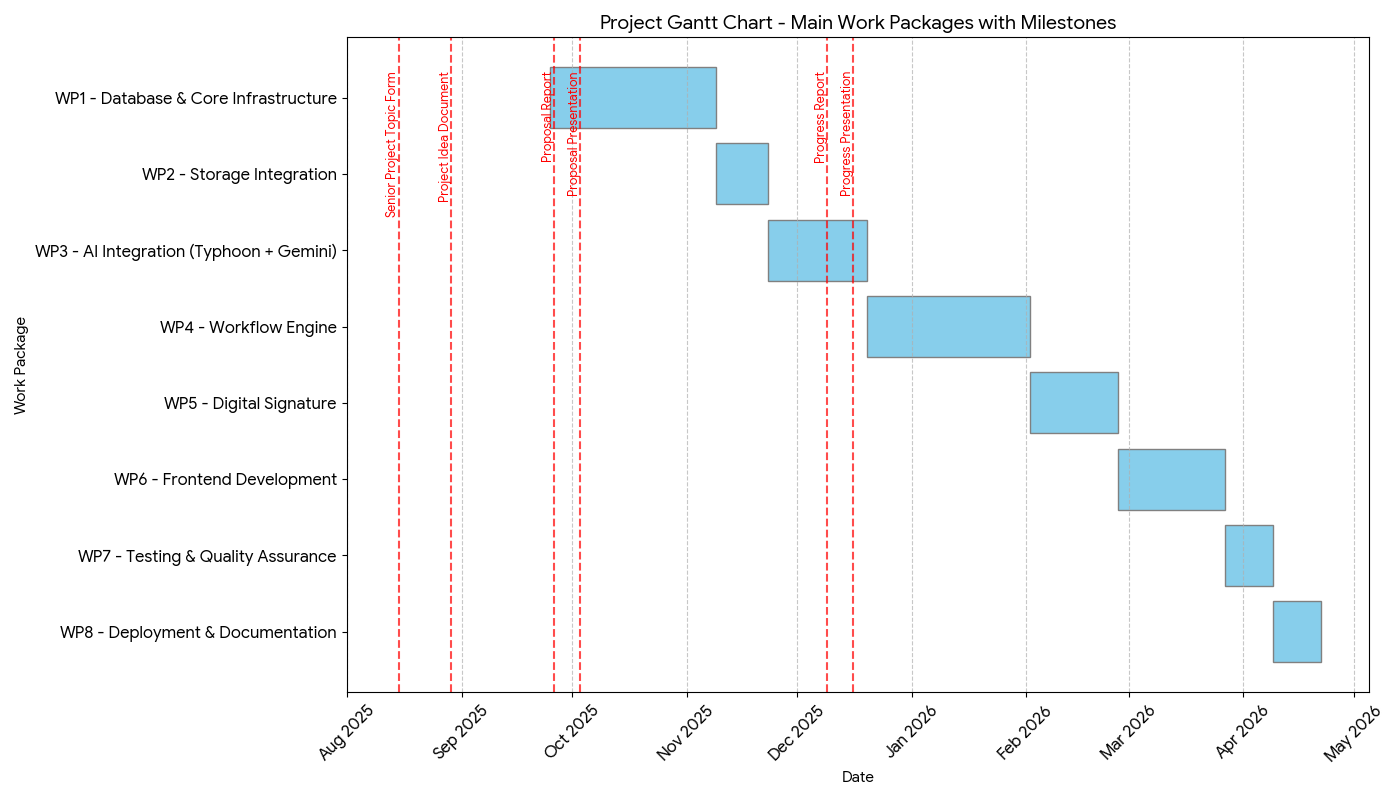
\includegraphics[width=\linewidth]{image/Gantt_Main_WP.png}
\captionof{figure}{Overall Gantt chart for the AgentiX project work plan.}
\end{center}

\begin{center}
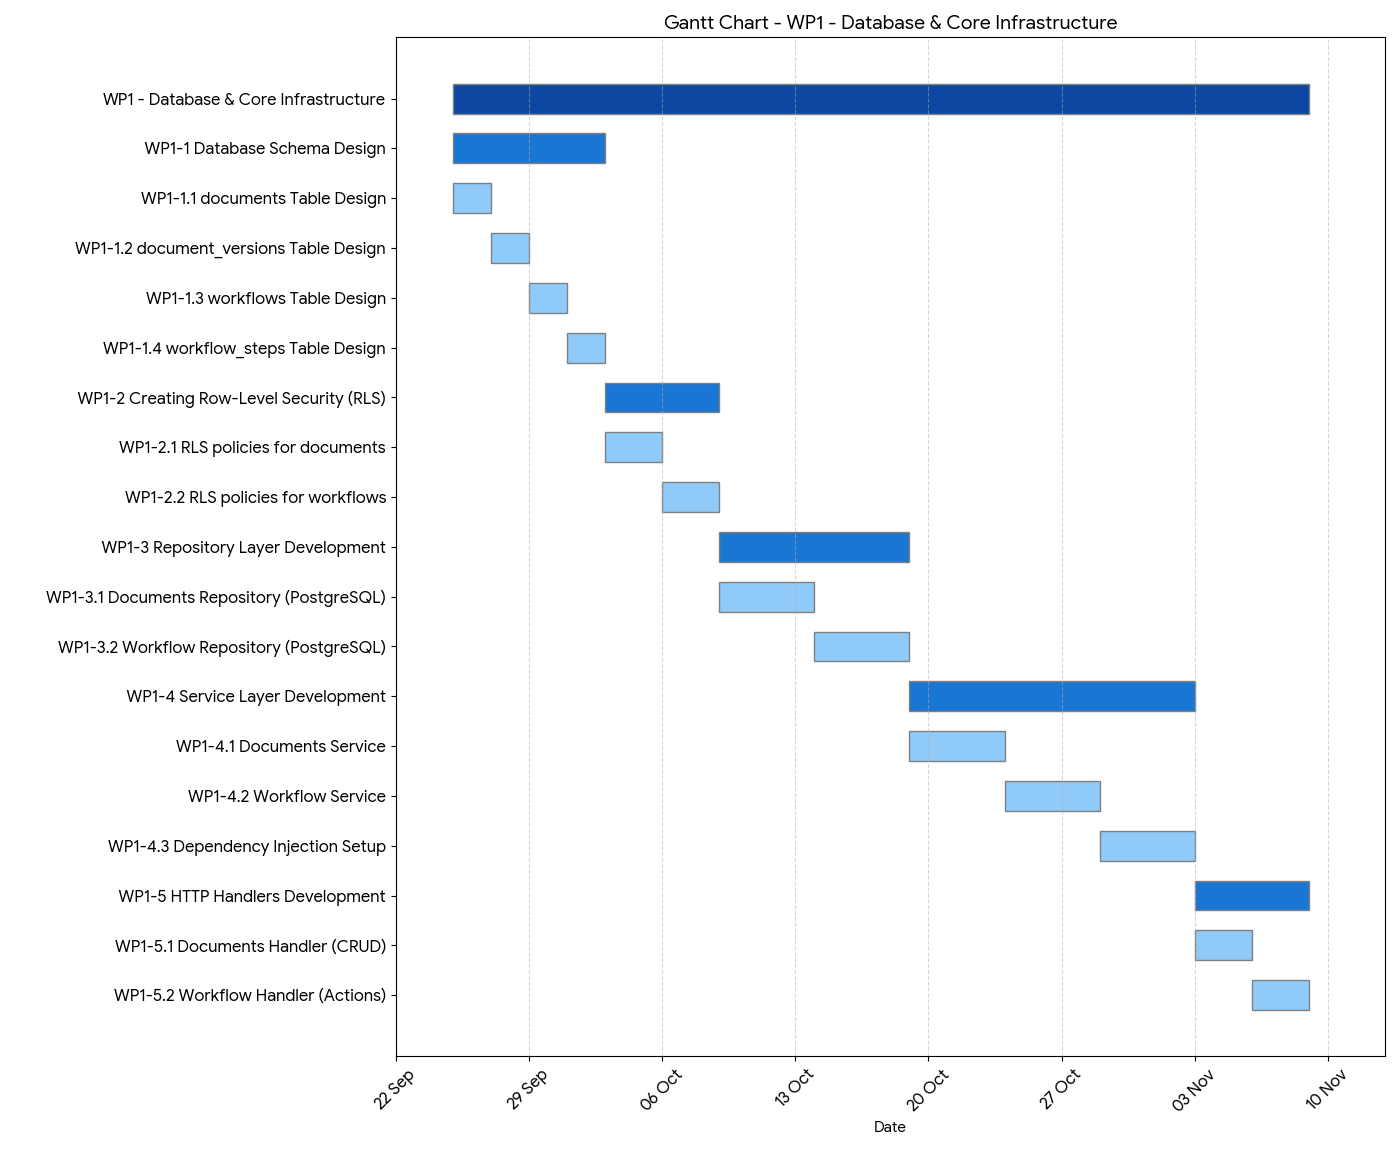
\includegraphics[width=\linewidth]{image/Gantt_WP1.png}
\captionof{figure}{Detailed schedule for Work Package 1.}
\end{center}

\begin{center}
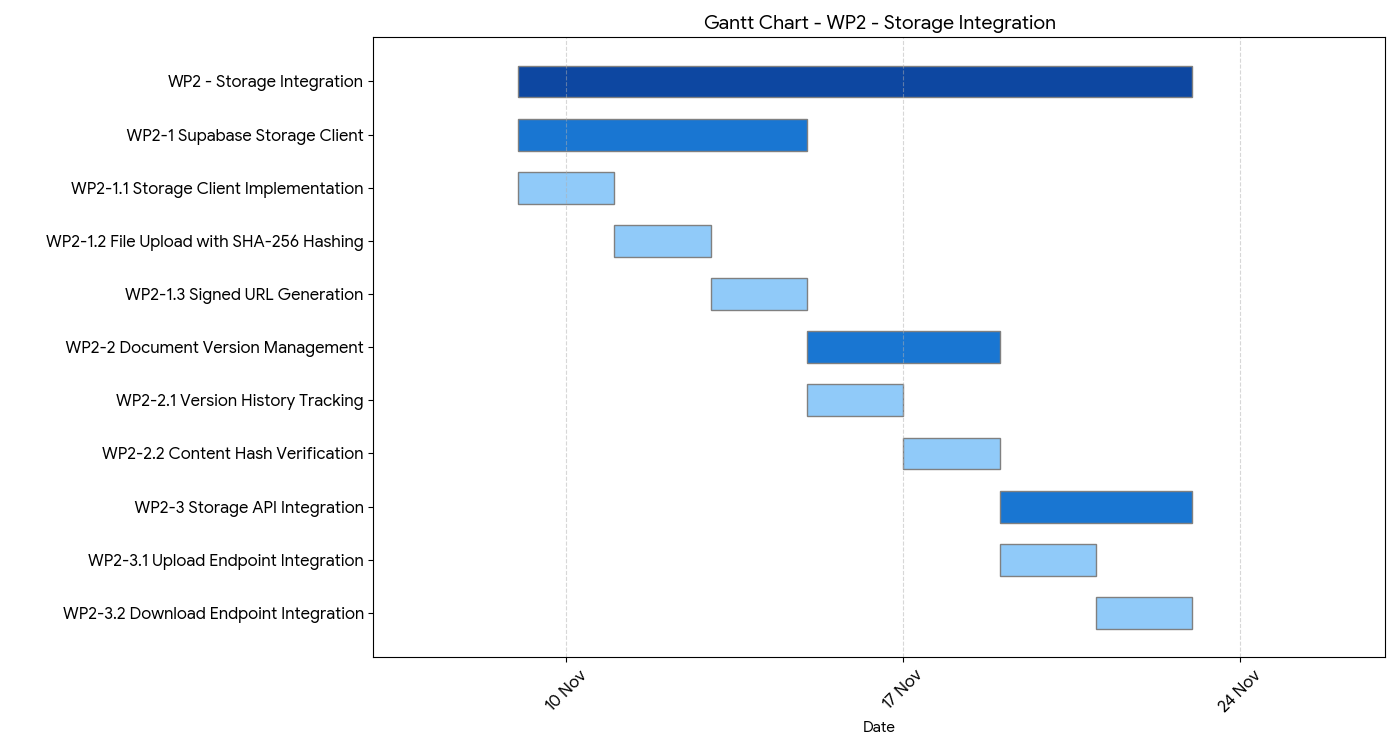
\includegraphics[width=\linewidth]{image/Gantt_WP2.png}
\captionof{figure}{Detailed schedule for Work Package 2.}
\end{center}

\begin{center}
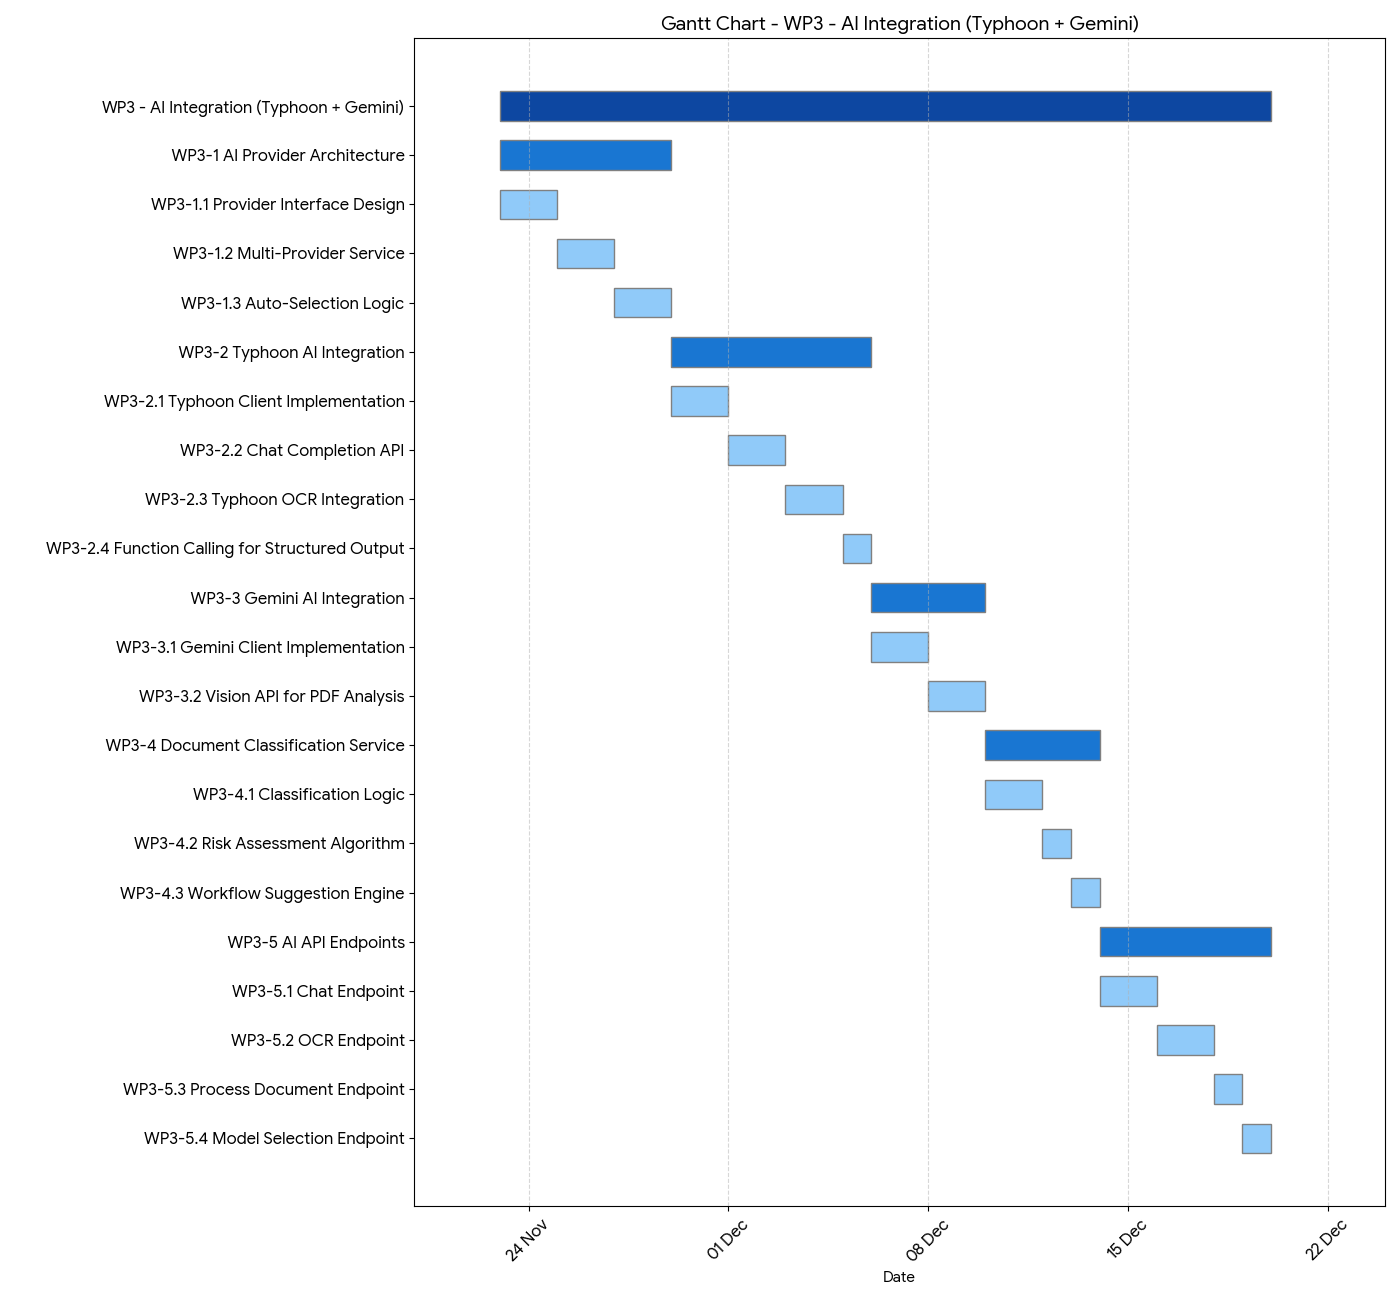
\includegraphics[width=\linewidth]{image/Gantt_WP3.png}
\captionof{figure}{Detailed schedule for Work Package 3.}
\end{center}

\begin{center}
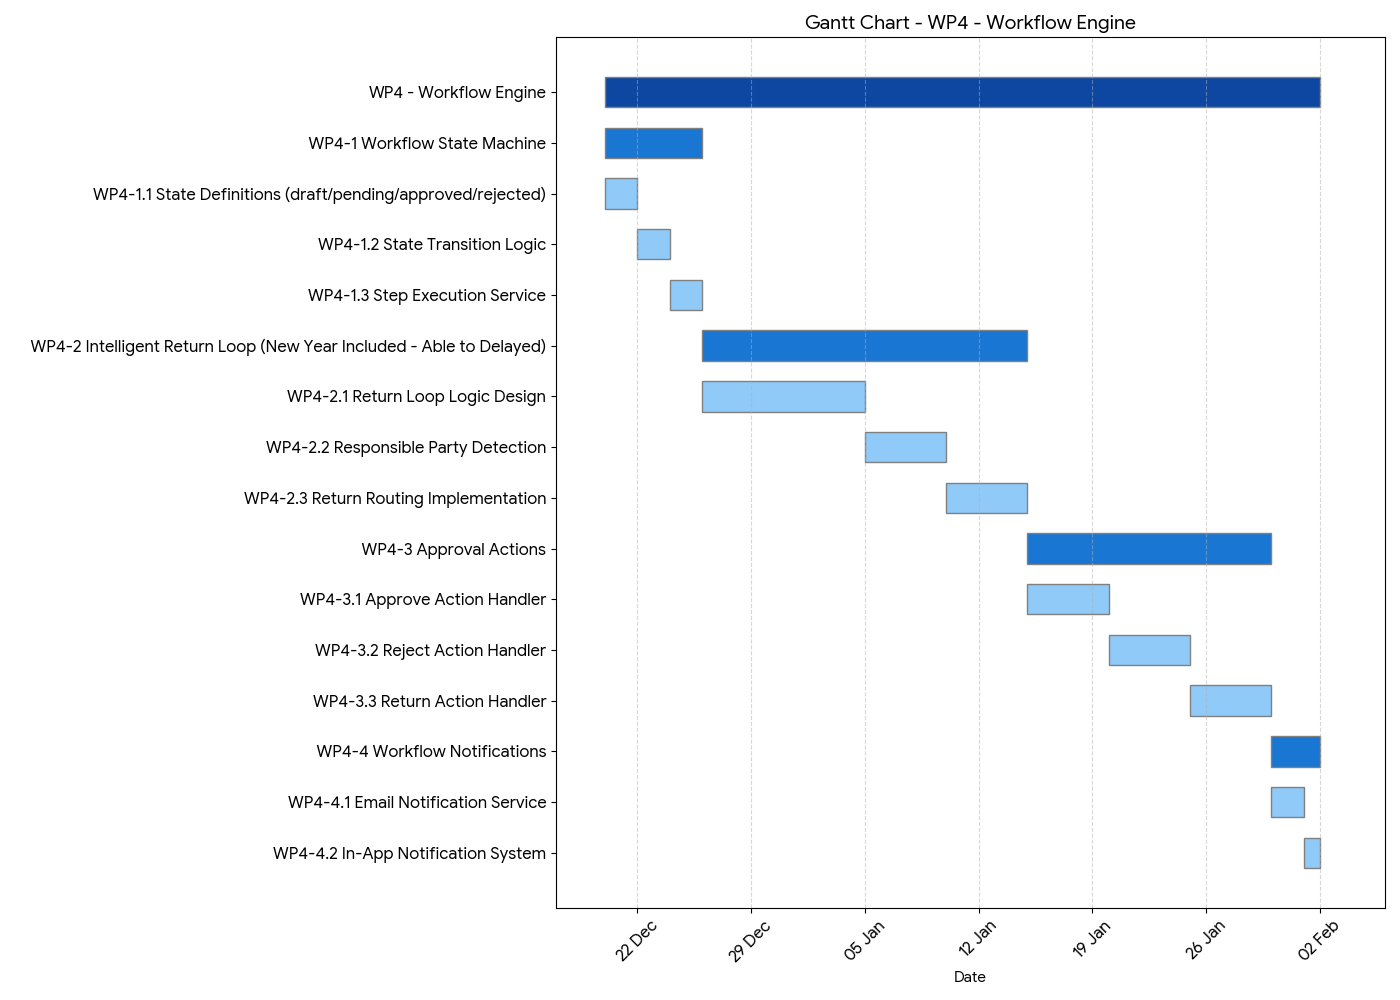
\includegraphics[width=\linewidth]{image/Gantt_WP4.png}
\captionof{figure}{Detailed schedule for Work Package 4.}
\end{center}

\begin{center}
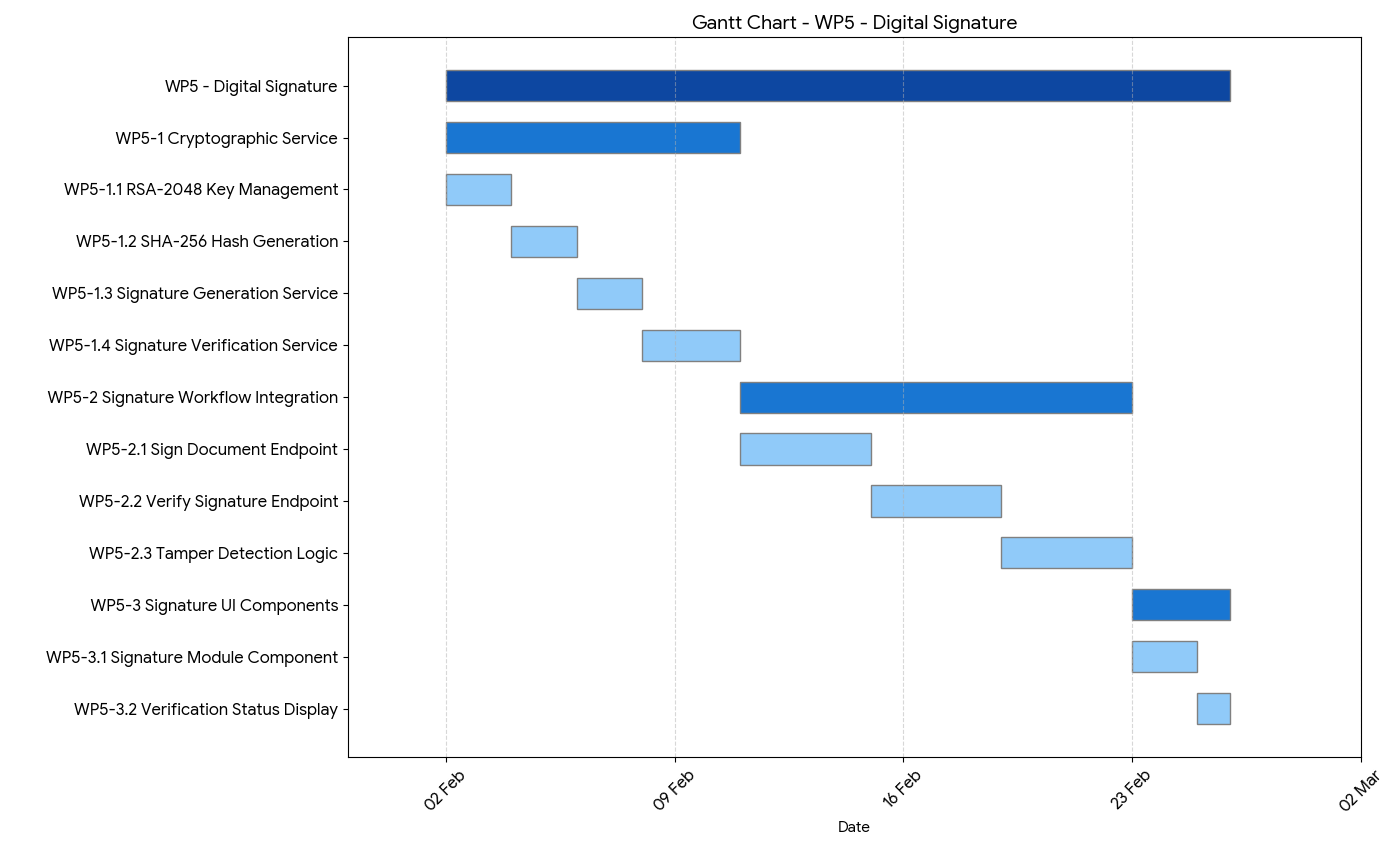
\includegraphics[width=\linewidth]{image/Gantt_WP5.png}
\captionof{figure}{Detailed schedule for Work Package 5.}
\end{center}

\begin{center}
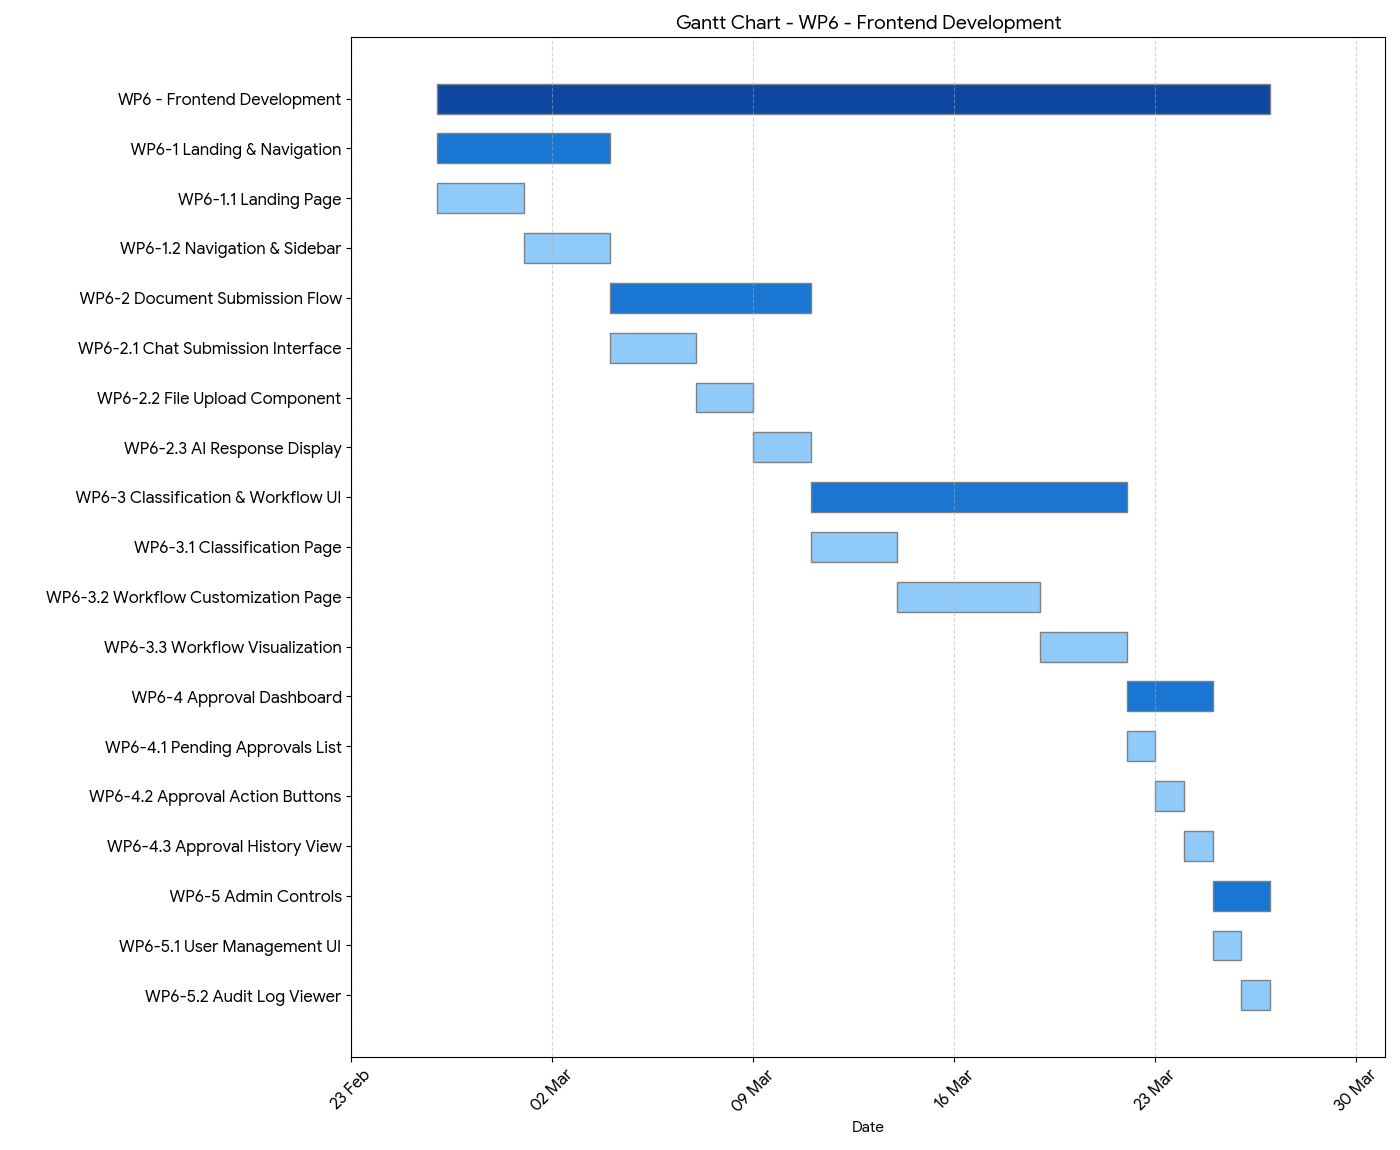
\includegraphics[width=\linewidth]{image/Gantt_WP6.png}
\captionof{figure}{Detailed schedule for Work Package 6.}
\end{center}

\begin{center}
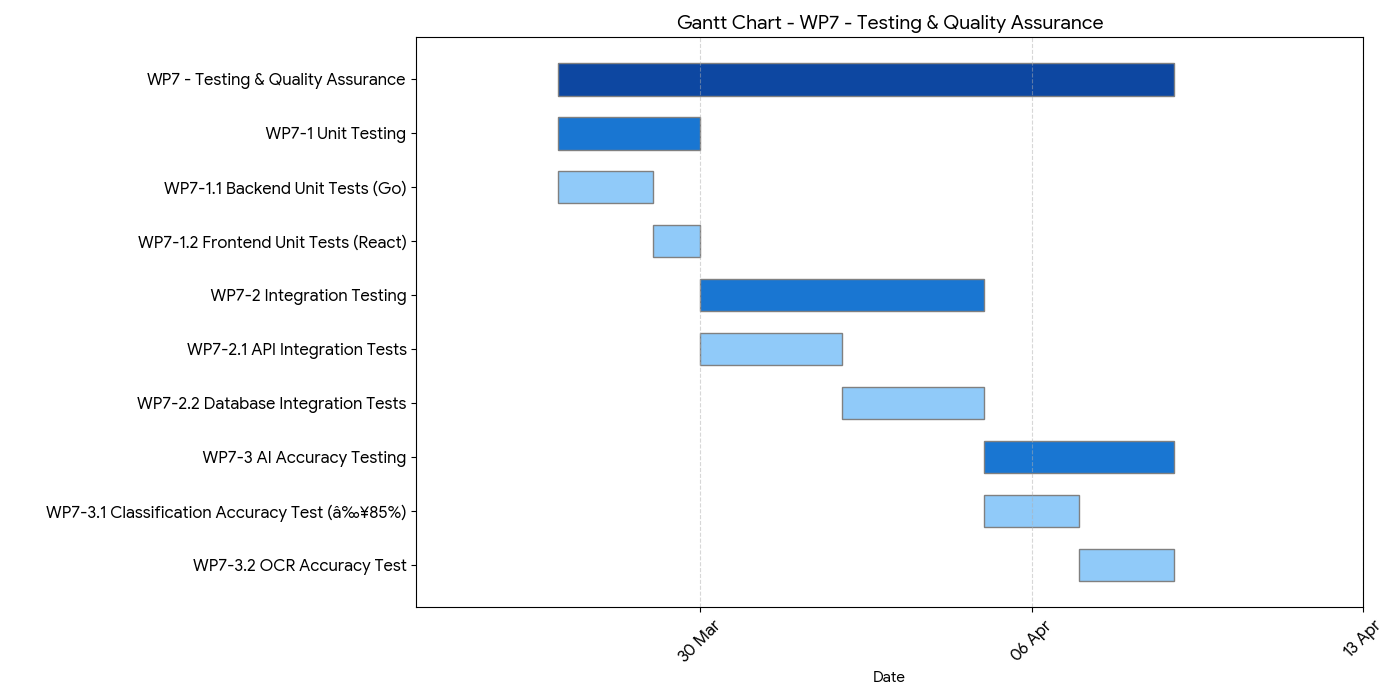
\includegraphics[width=\linewidth]{image/Gantt_WP7.png}
\captionof{figure}{Detailed schedule for Work Package 7.}
\end{center}

\begin{center}
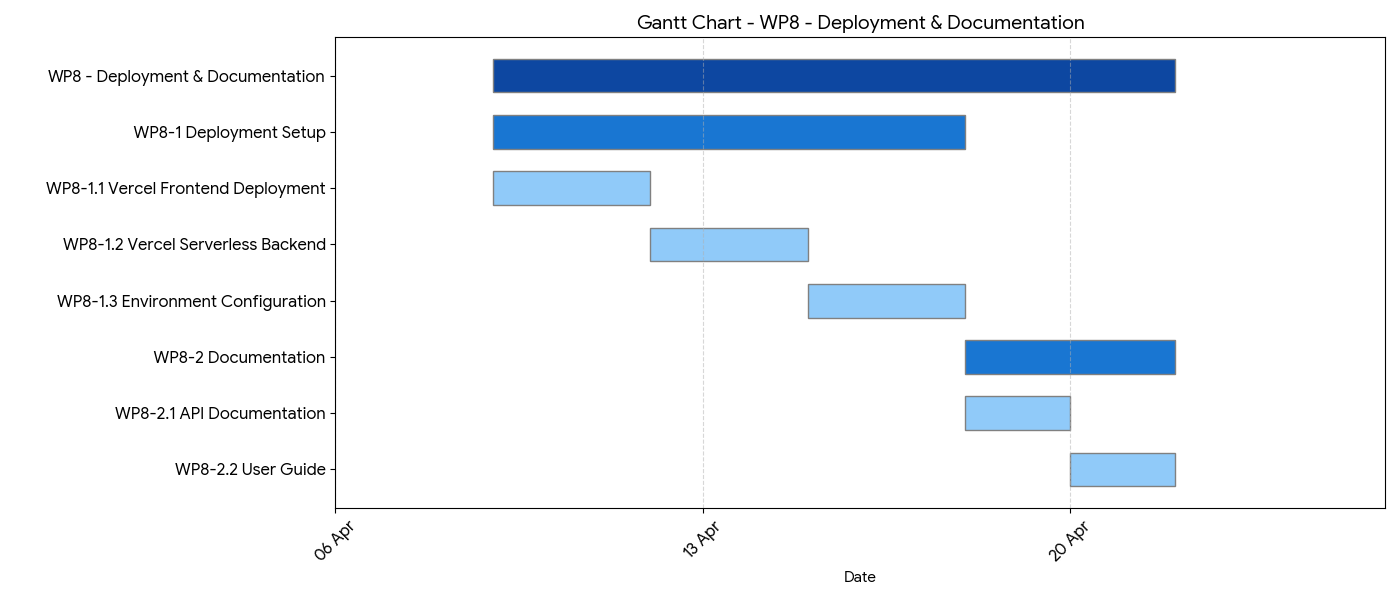
\includegraphics[width=\linewidth]{image/Gantt_WP8.png}
\captionof{figure}{Detailed schedule for Work Package 8.}
\end{center}

\newpage

\chapter{Background Theory and Related Work}

The proposed AgentiX platform sits at the intersection of several
established and emerging fields of research: intelligent document
processing, business process automation, and cryptographic security. A
review of existing literature reveals a strong academic and industrial
consensus on the challenges of manual workflows and the transformative
potential of artificial intelligence (AI) in this domain, while also
highlighting key areas requiring robust solutions. This review will
cover advancements in these areas, considering both proprietary and
open-source approaches.

\vspace{1em}

\section{Theoretical Foundations and Literature Review}

\subsection{Artificial Intelligence (AI)}

Artificial Intelligence (AI) refers to computer systems that perform
tasks normally associated with human cognition, such as perception,
language understanding, reasoning, prediction, and decision-making. In
modern software systems, AI is usually implemented through data-driven
models that learn patterns from examples rather than relying only on
hand-written rules. For AgentiX, AI provides the foundation for document
classification, approval routing, anomaly detection, and intelligent
recommendation of workflow actions.

AI can be understood as a broad discipline that includes machine
learning, natural language processing, computer vision, knowledge
representation, optimization, and decision support. Different AI
techniques are suitable for different types of problems. Rule-based AI
works well when conditions are explicit and stable, while statistical or
machine learning approaches are better for problems involving uncertain,
unstructured, or highly variable input. Because organizational documents
often vary in format, wording, and level of formality, a flexible AI
approach is especially important in the AgentiX platform.

In practical enterprise systems, AI is valuable not only because it can
automate tasks, but also because it can reduce cognitive load for human
users. Instead of forcing staff to review every document manually, AI
can pre-classify incoming files, highlight relevant sections, identify
missing information, and recommend the most appropriate next step in the
approval chain. This creates a hybrid human-AI workflow in which routine
analysis is accelerated while important decisions remain under human
control. Such a model is particularly suitable for approval systems,
where accuracy, accountability, and traceability are as important as
speed.

For this reason, AI in AgentiX is not treated as an isolated feature but
as an enabling layer across the whole system. It supports document
understanding at the input stage, workflow reasoning during routing, and
exception detection when something unusual occurs. By combining these
capabilities, the platform can respond more intelligently to real-world
organizational complexity than a purely manual or rule-only system.

\vspace{1em}

\subsection{Transformers}

Transformers are a neural network architecture designed around
self-attention, which allows a model to evaluate relationships between
all parts of an input sequence at the same time. This makes them more
effective than older recurrent architectures for handling long text,
preserving context, and scaling to large datasets. Transformers are now
the basis of most modern large language models (LLMs), and they are
especially relevant to AgentiX because they support document
understanding tasks such as semantic classification, key-phrase
extraction, summarization, and question answering over approval
documents.

The key innovation of the transformer architecture is its ability to
represent contextual meaning by assigning different levels of attention
to different words, sentences, or document segments. Unlike sequential
models that process text strictly from left to right, transformers can
capture long-range dependencies more efficiently. This is highly useful
for formal documents, where the meaning of a clause may depend on terms
defined several paragraphs earlier. In approval workflows, such context
sensitivity is important because small differences in wording may change
a document's category, urgency, or approval path.

Another important advantage of transformers is their adaptability. A
pretrained transformer model can learn general language structure from
large corpora and then be fine-tuned for more specific tasks. In the
context of AgentiX, this means a general language model can be adapted
for enterprise documents, contracts, requests, memoranda, or policy
forms. The same underlying architecture can therefore support multiple
functions within one platform, reducing the need to build separate
special-purpose models for each task.

Transformers also play a central role in retrieval, summarization, and
structured output generation. For example, a transformer-based model may
extract relevant document fields, summarize the main purpose of a
submission, or generate a recommended workflow explanation for the user
or approver. These capabilities improve system transparency because the
platform does not merely classify a document; it can also communicate
why a particular route or recommendation was produced. This is valuable
in enterprise environments where explainability supports trust and user
acceptance.

\vspace{1em}

\subsection{Generative AI}

Generative AI refers to models that create new content by learning
patterns from large datasets. In the context of AgentiX, generative AI
is used to interpret unstructured documents, extract key semantic
signals, and propose structured workflow decisions. Unlike traditional
rule-based automation, generative models can reason over language,
summarize complex material, and provide explanations for their outputs.
This capability is essential for document approval systems, where
documents vary in format, writing style, and intent. Generative AI
enables the platform to transition from static routing rules to
context-aware workflow orchestration, while still allowing human
approvers to validate and override decisions.

\subsubsection{Large Language Models and their Multimodal Capabilities}

Large Language Models (LLMs) are a class of generative AI systems trained
on massive text corpora. They excel at tasks such as classification,
summarization, semantic extraction, and question answering. Recent LLMs
extend these abilities beyond text to support multimodal inputs, such as
PDFs, scanned images, and mixed text–image documents. Multimodal LLMs can
interpret layout, tables, diagrams, and embedded text, which is critical
for real-world enterprise documents that are rarely plain text.

For AgentiX, multimodal capability is important because approval
documents often include signatures, stamps, scanned pages, and complex
formatting. By processing both visual and textual information, the model
can more accurately infer document type, identify relevant fields, and
propose suitable approval steps. Multimodal reasoning also reduces
dependency on separate OCR pipelines, improving reliability and
latency. At the same time, the system requires structured outputs
(function calling or schema-constrained responses) so that AI-generated
insights can be transformed into executable workflow steps. This
combination of language understanding, multimodal perception, and
structured response generation defines the role of LLMs within the
AgentiX workflow engine.

\subsubsection{Per-Model Specifications}

\begin{itemize}
  \item \textbf{gemini-3-pro-preview} (Google Gemini, default) \\
  \emph{Capabilities}: text, vision, pdf, function\_calling, thinking. \\
  \emph{Role in system}: This is the primary model for document
  understanding and approval workflow generation. Its multimodal
  capability allows the system to interpret PDFs that contain complex
  layout, tables, and embedded images without requiring an external OCR
  step. The function calling feature enables structured outputs for
  routing decisions, while the “thinking” capability improves reasoning
  in classification and risk assessment. Because of these advantages,
  this model is selected as the default for production use.

  \item \textbf{gemini-3-flash-preview} (Google Gemini) \\
  \emph{Capabilities}: text, vision, pdf, function\_calling, thinking. \\
  \emph{Role in system}: This model is optimized for lower latency and
  faster turnaround. It is suitable for interactive workflows where
  response time is critical, such as chat-style document submission or
  quick previews. It retains multimodal support and function calling,
  ensuring that structured workflow proposals remain consistent even
  under latency constraints. In the system design, it is used as a
  performance-focused alternative to the default Gemini model.

  \item \textbf{gemini-2.0-flash-exp} (Google Gemini) \\
  \emph{Capabilities}: text, vision, pdf, function\_calling. \\
  \emph{Role in system}: This model provides a stable, fast multimodal
  option and can be used as a fallback when newer Gemini models are
  unavailable or rate-limited. Although it lacks the explicit “thinking”
  tag, it still supports structured output and PDF vision, which is
  sufficient for many classification tasks. The system treats this model
  as a compatibility layer that preserves multimodal processing even
  under degraded conditions.

  \item \textbf{typhoon-v2.5-qwen3-30b-a3b-instruct} (SCB10X Typhoon) \\
  \emph{Capabilities}: text, function\_calling, Thai Context. \\
  \emph{Role in system}: This model is the primary Typhoon option for
  document analysis in Thai or mixed Thai-English contexts. It is used
  when Gemini is unavailable or when Thai-specific language handling is
  required. The function calling capability makes it suitable for
  returning structured approval steps, and its Thai optimization
  supports accurate classification of local-language documents. In the
  fallback architecture, this model ensures system continuity without
  sacrificing structured output quality.

  \item \textbf{typhoon-v1.5x-70b-instruct} (SCB10X Typhoon) \\
  \emph{Capabilities}: text, function\_calling, Thai Context. \\
  \emph{Role in system}: This model provides higher capacity for deeper
  text reasoning and is preferred when document complexity is high or
  when longer context is required. Its size makes it suitable for
  nuanced interpretation of complex contracts or policy documents. In
  the system, it can be selected for high-stakes workflows where deeper
  semantic understanding is more important than cost or latency.

  \item \textbf{typhoon-v1.5-instruct} (SCB10X Typhoon) \\
  \emph{Capabilities}: text, function\_calling, Thai Context. \\
  \emph{Role in system}: This model is a lighter-weight Typhoon option
  for routine classification and cost-efficient inference. It is useful
  for simple documents or high-volume processing where performance and
  budget constraints matter. While it is smaller than the 70B variant,
  it still supports structured responses and Thai-language capability,
  making it a practical default for basic workflows in Thai contexts.
\end{itemize}

\vspace{1em}

\subsection{Agents}

An agent is a system that can observe its environment, maintain some
internal state or goal, and choose actions that move it toward a target
outcome. In software engineering, agents may be simple rule-based
automations or more advanced systems that combine sensing, reasoning,
and action. The important feature is autonomy: an agent does not merely
produce an output, but can decide what to do next based on the current
state of the task. In a workflow context, an agent can inspect a
submitted document, identify the next required approver, and trigger the
appropriate system action.

The concept of agency becomes especially important when a system must
operate across multiple stages rather than perform only a single
prediction. A conventional AI model might classify a document one time
and stop there. An agent-oriented system, by contrast, can use that
classification as one part of an ongoing process: it can evaluate the
result, compare it with workflow rules, determine whether additional
information is needed, and then choose the next operational step. This
stepwise, goal-directed behavior makes agent-based systems a strong fit
for approval platforms, where tasks unfold over time and involve dynamic
interaction between users, documents, and organizational roles.

Agents can also be designed with different levels of sophistication.
Some operate with fixed rules and deterministic triggers, while others
combine rule-based constraints with probabilistic reasoning from AI
models. In AgentiX, this distinction is useful because enterprise
processes often require both flexibility and control. For example, an
agent may use AI to estimate the document type or urgency, but still
apply organizational policy rules to ensure that the final route follows
authorized approval structures. In this way, agents help bridge the gap
between intelligent analysis and dependable operational execution.

From a system design perspective, agents also improve modularity. A
document-analysis agent, a routing agent, a notification agent, and a
verification agent may each handle different responsibilities while
contributing to one coordinated workflow. This modular decomposition
supports scalability, maintainability, and future enhancement. It also
aligns well with the AgentiX vision of an Agentic AI platform, where
intelligence is not limited to isolated predictions but is embedded in
the orchestration of the full approval lifecycle.

\vspace{1em}

\subsection{AI Agents}

AI agents extend the idea of agents by using AI models for perception,
reasoning, and decision-making. They typically combine a language model
with tools such as search, retrieval, databases, or workflow APIs so the
system can interpret a request, gather missing context, and act on the
result. Compared with static automation scripts, AI agents are better
suited to unstructured problems because they can reason over text,
adapt to new inputs, and operate across multiple steps. In AgentiX, an
AI agent can analyze the content of a document, infer its category,
compare it with policy rules, and recommend the correct approval path.

\vspace{1em}

\begin{figure}[htbp]
\centering
\resizebox{0.82\linewidth}{!}{%
\begin{tikzpicture}[
  node distance=1.2cm and 1.3cm,
  font=\small,
  box/.style={draw, rounded corners, align=center, minimum width=2.7cm, minimum height=0.85cm, fill=gray!8},
  smallbox/.style={draw, rounded corners, align=center, minimum width=2.3cm, minimum height=0.75cm, fill=blue!6},
  tool/.style={draw, rounded corners, align=center, minimum width=2.3cm, minimum height=0.75cm, fill=green!8},
  arrow/.style={->, thick}
]
\node[box] (user) {User / Document\\Submission};
\node[box, right=of user] (agent) {AI Agent\\Orchestrator};
\node[smallbox, above right=of agent] (llm) {LLM\\Reasoning \& Planning};
\node[tool, below right=of agent] (tools) {Tools\\OCR / Search / DB / APIs};
\node[box, right=of llm, yshift=-1.0cm] (out) {Action / Output\\Route, Reply, or Update};

\draw[arrow] (user) -- node[above, sloped] {input} (agent);
\draw[arrow] (agent) -- node[above, sloped] {context} (llm);
\draw[arrow] (llm) -- node[right] {tool call} (tools);
\draw[arrow] (tools) -- node[left] {results} (llm);
\draw[arrow] (llm) -- node[above, sloped] {decision} (out);
\draw[arrow] (agent) |- node[pos=0.25, right] {control loop} (tools);
\end{tikzpicture}%
}
\caption{Conceptual flow of an AI agent communicating with an LLM and external tools.}
\label{fig:ai-agent-llm-tools}
\end{figure}

Figure~\ref{fig:ai-agent-llm-tools} illustrates how an AI agent acts as
an orchestration layer between user input, reasoning capabilities, and
external operational tools. The process begins when a user or document
submission enters the system. The agent then interprets the request,
determines what information is needed, and passes the relevant context
to the language model. Rather than relying only on internal model
knowledge, the agent can call tools such as OCR services, enterprise
databases, search components, or workflow APIs to obtain current and
task-specific information. The results of those tool interactions are
returned to the reasoning layer, allowing the agent to refine its
understanding and select an appropriate next action.

This interaction pattern is important because it shows that intelligent
behavior in enterprise systems is not produced by language generation
alone. Effective AI agents depend on a feedback loop between reasoning
and action. In the context of AgentiX, such a loop allows the platform
to inspect document contents, verify related data, consult policy rules,
and then either route the file, request clarification, or return it for
revision. The figure therefore represents more than a technical model:
it explains why AI agents are suitable for approval workflows that must
adapt to incomplete information, multi-step decisions, and changing
organizational context.

\vspace{1em}

\subsection{Agentic AI}

Agentic AI describes a system in which one or more AI agents plan,
coordinate, and execute multi-step tasks with limited human supervision.
Unlike single-response AI systems that stop after producing a result,
agentic systems are process-oriented: they can break a goal into
subtasks, select tools, react to new information, and continue until the
task is complete or safely interrupted. This approach is central to
AgentiX, because the platform is designed to combine document analysis,
approval routing, compliance validation, and return-loop handling into a
single orchestrated workflow rather than a fixed rule chain.

A key distinction between conventional AI and Agentic AI lies in the
nature of control. Conventional AI often performs a single isolated
function, such as classification, prediction, or summarization, and then
returns the result to a user or application. Agentic AI goes beyond this
by managing a sequence of decisions over time. It can evaluate progress,
revise its strategy when new information appears, and invoke different
capabilities depending on the current state of the task. In this sense,
Agentic AI is not simply a smarter model, but a more complete operating
paradigm for intelligent software.

This paradigm is particularly important in business workflows because
real organizational processes are rarely linear. A submitted document
may be incomplete, routed to the wrong department, missing supporting
evidence, or subject to special policy conditions. A static workflow
engine typically requires every exception to be anticipated in advance
through manually encoded rules. By contrast, an agentic system can
handle variation more flexibly by combining reasoning, context lookup,
and policy-aware actions. This makes the workflow more adaptive while
still preserving oversight and control.

In AgentiX, Agentic AI can be understood as the coordination layer that
binds several system capabilities into one coherent approval process. A
document may first be interpreted using AI-based classification, then
checked against approval policies, then assigned to an appropriate
approver, and finally returned for revision or forwarded for signing
based on the resulting decision. Each of these steps may involve a
combination of AI reasoning and deterministic business rules. The
agentic approach is valuable because it helps the system move from one
stage to the next in a context-aware way instead of treating each module
as a disconnected component.

Another important characteristic of Agentic AI is iterative feedback.
The system can observe the outcome of an action and use that outcome to
inform the next step. For example, if a document is rejected, the system
can determine whether the issue concerns missing fields, incorrect
classification, policy non-compliance, or an incomplete approval chain.
Rather than restarting the entire process blindly, the agentic layer can
route the document back to the correct user with more specific guidance.
This supports one of the main goals of AgentiX, namely reducing delays
caused by inefficient manual rework and unclear handoff points.

Agentic AI also raises important design considerations related to
reliability, transparency, and governance. In enterprise settings,
autonomous decision support must be explainable enough for users and
administrators to trust it. For that reason, an effective agentic system
should log important actions, expose workflow reasoning where practical,
and remain bounded by explicit approval policies. In AgentiX, this means
Agentic AI should assist with orchestration and recommendation while
keeping high-stakes approval authority with authorized human roles. This
balance allows the platform to gain the efficiency of intelligent
automation without compromising accountability.

From a broader perspective, Agentic AI represents the transition from
software that merely responds to commands toward software that can pursue
goals within controlled operational boundaries. That transition is highly
relevant to document approval, where the system must do more than store
files or display forms. It must interpret intent, coordinate roles,
manage sequence, and respond intelligently to exceptions. Therefore,
Agentic AI provides the conceptual foundation for AgentiX as an
intelligent workflow orchestration platform rather than a simple digital
document portal.

\vspace{1em}

\subsection{The Evolution of Business Process Automation (BPA)}

Traditional business process automation (BPA), often relying on Robotic
Process Automation (RPA), has been effective in handling repetitive,
rule-based tasks with structured data. However, as noted by research
from
 and
, these systems are rigid and fail when faced with unstructured
data or unexpected exceptions. This limitation has spurred the
development of more advanced systems, termed "Agentic AI workflows"
(UiPath, 2025). These systems are defined by their ability to reason,
plan, and adapt dynamically without constant human intervention. The
AgentiX project builds directly on this new paradigm, moving beyond
simple automation to create a truly intelligent and flexible workflow.

\vspace{1em}

\subsection{Intelligent Document Processing (IDP) and Natural Language
Processing (NLP)}

The core of AgentiX\textquotesingle s intelligent routing relies on
Intelligent Document Processing (IDP). A wealth of literature, including
studies from
 and
, confirms that IDP, powered by AI technologies such as Natural
Language Processing (NLP), Machine Learning (ML), and Optical Character
Recognition (OCR), is crucial for automating document-heavy processes.
These studies highlight that NLP can accurately classify documents,
extract key data from unstructured text (e.g., invoices, contracts), and
enable intelligent, context-aware routing. The challenge, as documented
by
, often lies in the quality and standardization of training
data. AgentiX addresses this by focusing its Proof of Concept (PoC) on a
clean, consistent dataset to validate the feasibility of its AI core.

\vspace{1em}

\subsection{Digital Signatures and Cryptographic Integrity}

The legal and security aspects of digital signatures are
well-documented. Research from
 and a comprehensive guide from
 confirm that digital signatures, which are a specific type of
electronic signature, use cryptographic methods based on Public Key
Infrastructure (PKI) and hash functions to guarantee document integrity,
authenticity, and non-repudiation. Any alteration to a digitally signed
document invalidates the signature, providing a robust security
mechanism. AgentiX's use of "bit-matching" is a direct application of
this established cryptographic principle to ensure the immutability of
signed documents. Case studies from
 further demonstrate the successful implementation of secure
digital signing solutions to streamline paperless workflows.

\vspace{1em}

\section{Open-Source Tools and Frameworks}

The development of AI-powered solutions can be pursued with both
proprietary and open-source toolkits. A growing body of research
supports the viability of open-source frameworks for key project
components. For \textbf{NLP and document processing}, frameworks like
\textbf{Hugging Face\textquotesingle s Transformers} and libraries such
as \textbf{spaCy} offer powerful, pre-trained models for tasks like text
classification and named entity recognition. These tools can be
fine-tuned on a custom dataset, providing a robust, flexible alternative
to proprietary API services. For \textbf{workflow orchestration},
open-source libraries like \textbf{LangChain} and \textbf{AutoGen}
provide the foundational architecture for building multi-agent systems
that can reason and perform multi-step tasks. In the realm of
\textbf{cryptography and digital signatures}, open-source libraries like
\textbf{OpenSSL} and \textbf{PyCryptodome} provide the necessary tools
for implementing secure hashing functions and managing public-key
infrastructure. The use of these open-source tools allows for greater
customization, transparency, and a reduction in long-term licensing
costs, though it may require a higher initial investment in development
expertise.

\subsection{Challenges in Implementation and User Adoption}

While the technical capabilities are promising, academic and industry
literature consistently points to several challenges in implementing
automation in large organizations. These include employee resistance to
change, integration with legacy systems, and the need for clear
governance. A successful implementation requires a clear alignment
between business goals and the technological solution, as well as a
strong focus on change management. The AgentiX project addresses these
known challenges by proposing a PoC that includes stakeholder feedback
from the very beginning, ensuring the solution is not only technically
sound but also aligned with user needs and organizational realities.

\vspace{1em}

\subsection{Conclusion}

The literature provides a clear foundation for the AgentiX project,
validating the need for an intelligent, secure, and flexible document
approval platform. While the technical components are supported by
existing research, the project\textquotesingle s unique value
proposition lies in the seamless integration of an \textbf{Agentic AI}
to create a truly adaptive workflow that solves a critical business
problem. By combining established cryptographic security with
cutting-edge AI, leveraging both proprietary and open-source tools,
AgentiX is poised to deliver a solution that moves beyond traditional
automation to a new era of intelligent process management.

\vspace{1em}

\section{Existing Solutions \& Competitor Analysis}

The document-approval landscape is crowded with mature offerings. Enterprise e-signature leaders, collaboration suites, automation platforms, and open-source frameworks each solve portions of the approval problem. Interviews with prospective stakeholders and a literature scan reveal that none of these players blend contextual document understanding, adaptive routing, and tamper-evident signing inside a single governed platform. The following review revisits representative categories in depth before contrasting their strengths with the gaps AgentiX is engineered to close.

\vspace{1em}

\subsection{Enterprise-Grade Digital Signature Platforms (Adobe Acrobat Sign, DocuSign)}
These services dominate regulated industries because they ship hardened e-signature infrastructure, global legal compliance (eIDAS, ESIGN), identity verification, and granular audit trails. Their drag-and-drop authoring tools and integration packs (Salesforce, Microsoft 365, Google Workspace) make onboarding simple for business users. However, their routing logic is static: approvals flow along predefined chains configured by administrators. The systems cannot read a contract clause to dynamically identify the right legal reviewer, leaving content-aware orchestration outside the core product.

 \begin{figure}
     \centering
     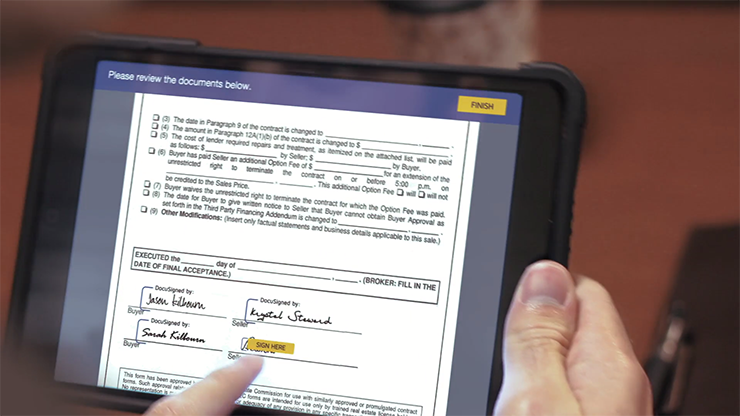
\includegraphics[width=0.5\linewidth]{image/DocuSign740.png}
     \caption{DocuSign}
     \label{fig:docusign}
 \end{figure}

\vspace{1em}

\subsection{Collaboration Suites (Lark, Google Workspace)}
Collaboration hubs streamline discussions, shared editing, and lightweight approval checklists, allowing teams to launch form-driven approvals directly inside chat and document tools. They work well for rapid feedback loops, but automation is limited to scripts or add-ons, and signature capabilities rely on third parties. Governance teams cite difficulties enforcing complex approval hierarchies or cryptographic controls across distributed tenants.

\begin{figure}
     \centering
     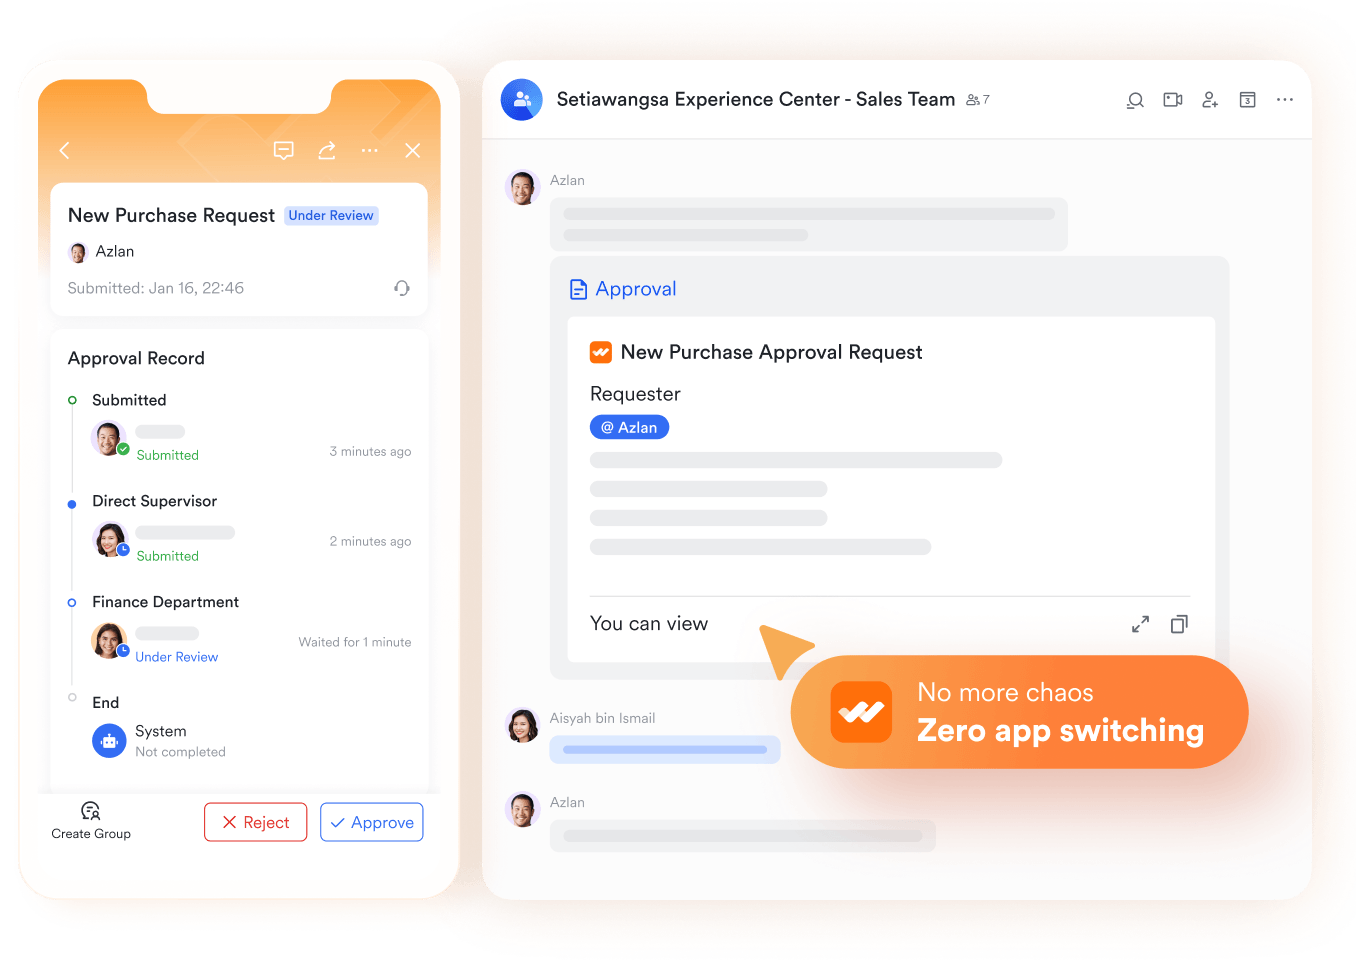
\includegraphics[width=0.5\linewidth]{image/lark_approval.png}
     \caption{Lark Approval}
     \label{fig:lark-approval}
\end{figure}

\newpage

\subsection{Automation Suites (Microsoft Power Automate)}
Power Automate offers a vast connector library and a low-code builder for trigger-based flows, accelerating integration projects inside Microsoft-centric organisations. Nevertheless, every routing rule remains human-authored; AI assistance is optional, and signature operations usually call external services. Maintaining consistent governance across multiple environments becomes burdensome in enterprise deployments.

\begin{figure}
     \centering
     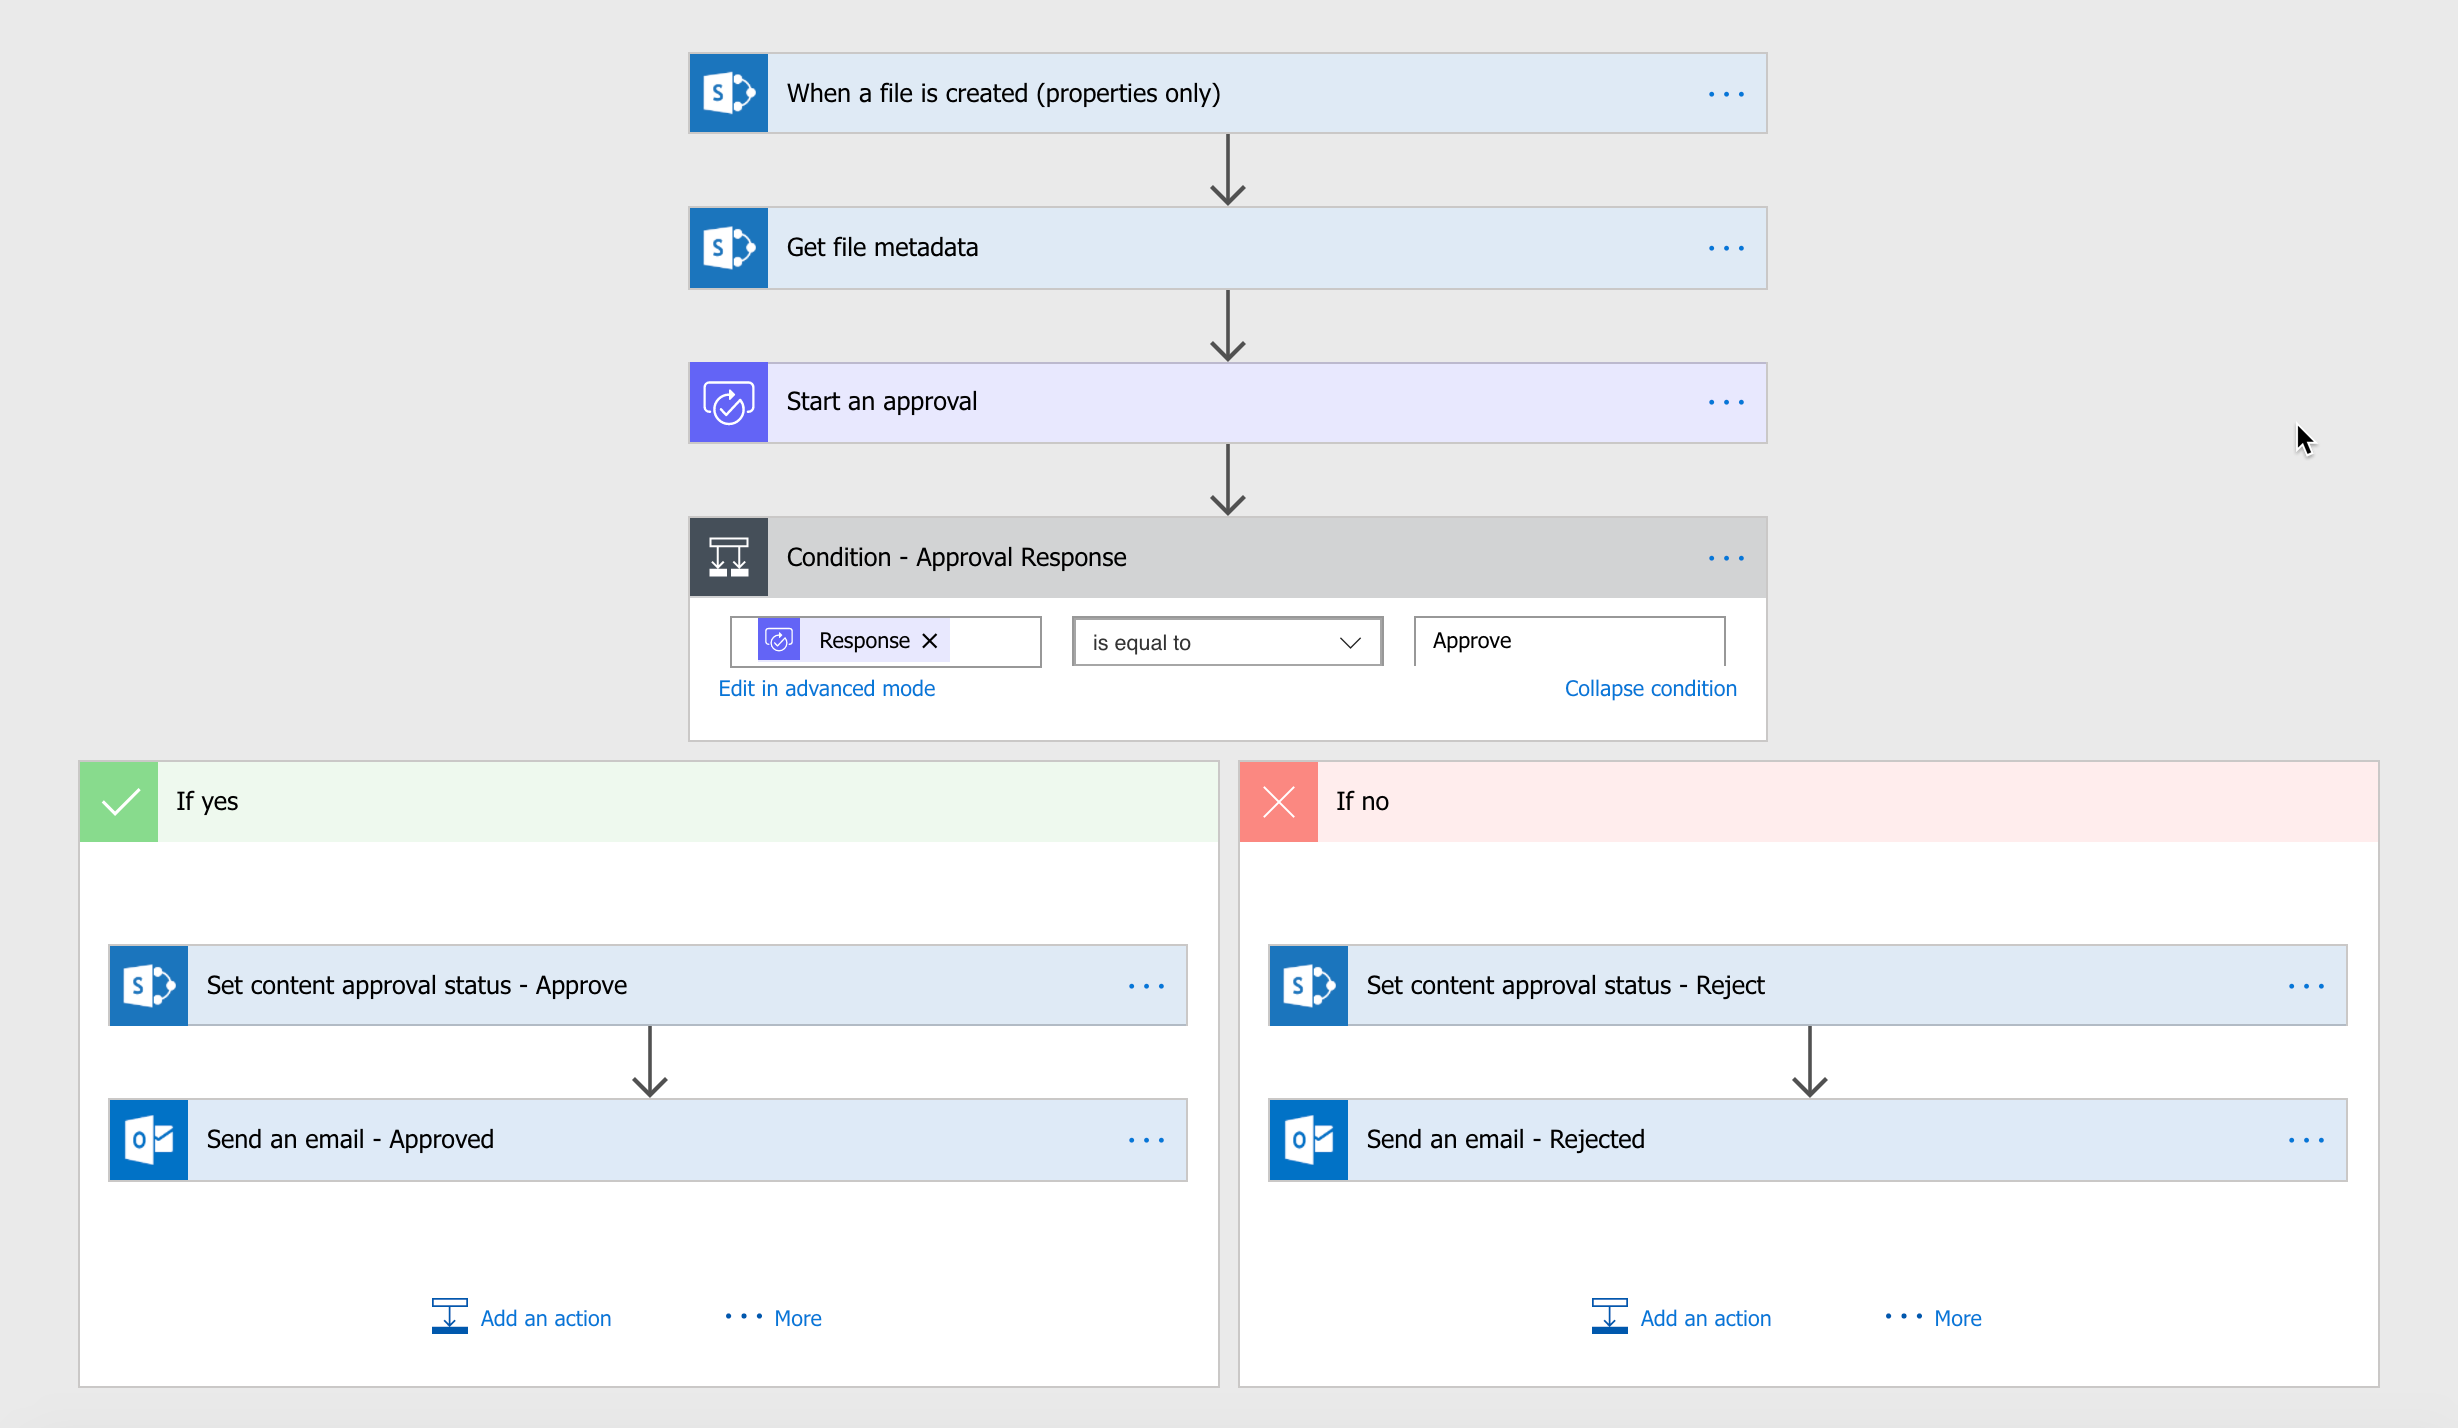
\includegraphics[width=0.5\linewidth]{image/flow-content-approval-full.png}
     \caption{Document Approval Workflow Example from Power Automate}
     \label{fig:powerautomate-workflow}
\end{figure}

\vspace{1em}

\subsection{Integration-First BPM Tools (n8n)}
Modern BPM tools like n8n empower technical teams to compose deeply customised automations with branching logic, multi-level approvals, and AI-powered nodes. They shine when organisations need to stitch together bespoke workflows across hundreds of systems, and sample blueprints demonstrate sophisticated document approvals. Yet n8n ships without native signing, so compliance assurances must be bolted on. Document comprehension requires custom prompt engineering, and the security posture varies by hosting model, presenting a steep learning curve for non-technical stakeholders.

 \begin{figure}
     \centering
     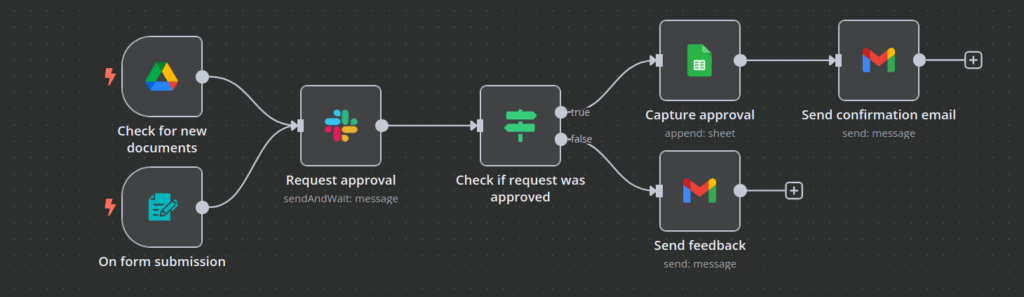
\includegraphics[width=0.5\linewidth]{image/approval_workflow-1024x297.png}
     \caption{Simple Flow of Document Approval on n8n}
     \label{fig:n8n-workflow}
 \end{figure}

\subsection{Open-Source Engineering Stacks}
Open-source stacks attract engineering-led organisations that demand maximum control and zero licensing fees. By mixing NLP models, workflow engines, and cryptography libraries, teams can theoretically recreate any capability. The trade-off is significant engineering effort: user interfaces, monitoring, compliance, and auditing must all be built and maintained internally, extending time-to-value and total cost of ownership.

\begin{table}[!htbp]
\centering
\renewcommand{\arraystretch}{1.25}
\begin{tabular}{|>{\raggedright\arraybackslash}p{0.24\textwidth}|>{\raggedright\arraybackslash}p{0.33\textwidth}|>{\raggedright\arraybackslash}p{0.34\textwidth}|}
\hline
\textbf{Solution Category} & \textbf{Strengths Observed} & \textbf{Gaps \& AgentiX Opportunity} \\ \hline
Enterprise digital signature platforms (Adobe Acrobat Sign, DocuSign) & Legal-grade signatures, identity verification, intuitive UX, broad integrations & Static routing; no AI-driven document interpretation; limited automation beyond signing \\ \hline
Collaboration suites (Lark, Google Workspace) & Real-time co-authoring, chat-driven approvals, templates and reminders & Lightweight automation; signature handled by add-ons; hard to enforce compliance-heavy flows \\ \hline
Automation suites (Microsoft Power Automate) & Low-code builder, extensive connectors, event-driven workflows & Manual rule design; optional AI; third-party signing; fragmented governance \\ \hline
Integration-first BPM tools (n8n) & Custom multi-step flows, conditional logic, AI nodes for classification & No native signing; document awareness must be engineered; security varies by deployment \\ \hline
Open-source engineering stacks & Full customisation, no licence costs, composable components (NLP, workflow, crypto) & High build/maintenance burden; compliance and auditing remain in-house responsibilities \\ \hline
\end{tabular}
\end{table}

Market feedback from stakeholder interviews converged with secondary research, so we condensed the capability coverage into a comparative matrix (Table~\ref{tab:market-comparison}) to visualise differentiation across popular platforms.
\begin{table}[!htbp]
\centering
\caption{Market capability comparison across leading approval platforms.}
\label{tab:market-comparison}
\scriptsize
\setlength{\tabcolsep}{4pt}
\renewcommand{\arraystretch}{1.25}
\resizebox{\textwidth}{!}{%
\begin{tabular}{|>{\raggedright\arraybackslash}p{0.19\textwidth}|>{\raggedright\arraybackslash}p{0.13\textwidth}|>{\raggedright\arraybackslash}p{0.13\textwidth}|>{\raggedright\arraybackslash}p{0.13\textwidth}|>{\raggedright\arraybackslash}p{0.13\textwidth}|>{\raggedright\arraybackslash}p{0.13\textwidth}|>{\raggedright\arraybackslash}p{0.13\textwidth}|}
\hline
\textbf{Capability} & \textbf{AgentiX} & \textbf{Moxo} & \textbf{Lark} & \textbf{Power Automate} & \textbf{Google Workspace} & \textbf{n8n} \\ \hline
Centralised approval hub & Native, agent-driven workspace & Client-facing collaboration suites & Built-in Approval app & Approval flows and staged routing & Docs approval requests & Custom multi-step workflows \\ \hline
Agentic/AI workflow automation & LLM-informed routing with policy context & Human-in-the-loop automation & Configuration-driven, manual logic & Power Automate AI optional add-ons & Limited Apps Script automation & AI nodes and agents for classification \\ \hline
Secure digital signatures & Bit-matching signatures plus credential validation & Legally binding e-signatures & Integrated e-sign support & Third-party signature connectors & Third-party signature integrations & Via integrations (DocuSign, etc.) \\ \hline
End-to-end lifecycle tracking & Submission-to-archive governance with audit trails & Managed workspace history & Versioning and status dashboards & Flow run history and analytics & Activity logs within Google Drive & Workflow diff and change history \\ \hline
Notification and escalation & SLA-aware alerts, intelligent return loop & Client alerts and reminders & Real-time chat notifications & Adaptive notifications via connectors & Email reminders & Messaging integrations, conditional reminders \\ \hline
Document intelligence & NLP classification, policy alignment & Metadata-driven filters & Manual rules or integrations & AI Builder add-ons & Limited structured metadata & AI-enhanced extraction pipelines \\ \hline
Governance flexibility & Cloud and private deployments, IAM alignment & Managed SaaS, vendor-controlled & SaaS within collaboration suite & Tenant-bound environments & Google Workspace tenant controls & Self-hosted or cloud deployment \\ \hline
\end{tabular}
}
\end{table}

\newpage

Key takeaways from the competitor analysis are:

\begin{itemize}
\item Enterprise leaders deliver trust and compliance, yet approvals remain static and sender-driven.
\item Collaboration and automation suites accelerate communications but lack deep signature validation or AI-driven routing.
\item Flexible BPM frameworks enable powerful integrations, although organisations must assemble security, data governance, and document intelligence on their own.
\end{itemize}

These gaps expose an opportunity for AgentiX to couple document understanding, adaptive routing, credential-aware signing, and lifecycle analytics in one governed platform.\sloppy

\newpage

\chapter{Proposed Work}

The analysis of existing solutions reveals critical gaps in the document approval market: static routing logic, fragmented security models, limited AI integration, and complex multi-vendor dependencies. AgentiX is engineered to bridge these gaps through an integrated platform that transforms the fundamental approach to organizational approval workflows.

\vspace{0.3cm}

\section{Core Solution Components}

AgentiX addresses the identified weaknesses through four interconnected architectural pillars:

\textbf{Web Application Layer}
A unified interface replaces the disparate tools organizations currently juggle. Unlike collaboration suites that handle approvals as an afterthought, or BPM tools that require technical expertise, AgentiX provides purpose-built submission portals, approval dashboards, and administrative controls designed specifically for document lifecycle management.

\textbf{Agentic AI Pipeline}
Where existing platforms rely on manual routing rules, AgentiX deploys multi-agent reasoning systems that analyze document content, classify obligations, and dynamically map approval paths. This eliminates the static routing limitations of enterprise signature platforms and the manual configuration burden of automation suites.

\textbf{Workflow Orchestration Engine}
The stateful orchestration engine coordinates sequential and parallel approvals while maintaining full audit trails. Unlike n8n's custom engineering requirements or Power Automate's fragmented governance, AgentiX provides out-of-the-box approval orchestration with policy alignment and SLA monitoring.

\textbf{Digital Signature Module with Bit-Matching}
Integrated cryptographic signing with tamper detection addresses the security gaps in collaboration platforms and the third-party dependencies in automation tools. Hardware-backed key custody and hash verification ensure legal defensibility without external signature services.

\vspace{2em}

\section{AgentiX Capabilities Addressing Market Weaknesses}

\begin{itemize}
\item
  \textbf{Agentic AI Workflow Orchestration}: Replaces the static routing of DocuSign and Adobe with multi-agent reasoning that classifies submissions, maps approvers, and sequences escalations without predetermined rules. This addresses the core limitation preventing existing platforms from handling complex, context-dependent approval scenarios.
\item
  \textbf{Document Understanding \& Routing Intelligence}: NLP pipelines normalize uploads and extract entities to enable content-aware routing from first submission. This eliminates the manual rule configuration required by Power Automate and the limited automation capabilities of collaboration suites.
\item
  \textbf{Intelligent Return Loop \& SLA Monitoring}: Routes rework directly to accountable owners and surfaces bottlenecks through dashboards, addressing the poor exception handling identified in existing approval systems. This prevents the endless email chains and lost documents that plague traditional workflows.
\item
  \textbf{Bit-Matching Digital Signature Module}: Hardware-backed keys with hash-based tamper detection provide cryptographic integrity without relying on third-party signature services. This addresses the security fragmentation and vendor dependencies that weaken current multi-tool approaches.
\item
  \textbf{Compliance-First Security Controls}: Role-based access, encryption, and immutable audit logs are built into the platform core, unlike the bolted-on security of open-source stacks or the tenant-dependent controls of collaboration suites.
\item
  \textbf{Flexible Deployment \& Integration Fabric}: Offers both managed cloud and private enterprise editions with pre-built connectors, addressing the deployment complexity of n8n and the vendor lock-in concerns of SaaS-only platforms.
\end{itemize}

\section{The AgentiX Value Proposition: Bridging the Gap}

AgentiX is designed to address the gaps identified in these existing
solutions. It integrates the core strengths of each category while
mitigating their weaknesses. It goes beyond the static routing of
enterprise digital signature platforms by incorporating a powerful
\textbf{Agentic AI} to provide true intelligent, dynamic workflows that
adapt to document content and context. Unlike "dumb" BPM tools,
AgentiX\textquotesingle s AI analyzes the document itself to inform its
routing decisions, making the workflow smarter and more autonomous from
the moment of submission. Finally, AgentiX offers a complete, integrated
solution that combines intelligent document analysis, workflow
automation, and cryptographic security in a single, user-friendly
platform, eliminating the need to build and maintain disparate systems
from scratch.

\vspace{1em}

\section{Conclusion}

While the existing market offers powerful tools for digital signatures
and workflow automation, no single solution fully addresses the need for
a system that is both highly secure and deeply intelligent.
Enterprise-grade platforms provide the trust and compliance required for
signatures but lack the dynamic, content-aware routing of AgentiX.
Conversely, while BPM tools and open-source frameworks offer
flexibility, they either require significant manual configuration or a
high technical investment to achieve the desired level of intelligence.
AgentiX\textquotesingle s proposed solution is a unique, hybrid model
that marries the robust security and compliance of digital signature
leaders with the intelligent, context-aware automation found in
cutting-edge AI research. This combination creates a new class of
product that is both powerful and practical for modern enterprise needs,
delivering a level of efficiency and security that current solutions
cannot match.

\newpage

\chapter{System Design}

This section presents the comprehensive technical architecture of AgentiX, detailing how the platform's components integrate to deliver secure, intelligent document approval workflows. The architecture follows microservices principles with security-first design patterns, ensuring scalability, maintainability, and regulatory compliance.

\vspace{1em}

\section{Software Engineering Diagram}

This section consolidates the core software engineering diagrams used to describe system behaviour, data movement, object structure, and interaction flow in AgentiX.

\subsection{Data Flow Diagrams}

\subsubsection{DFD Level 0 (Context Diagram)}

\begin{figure}[htbp]
\centering
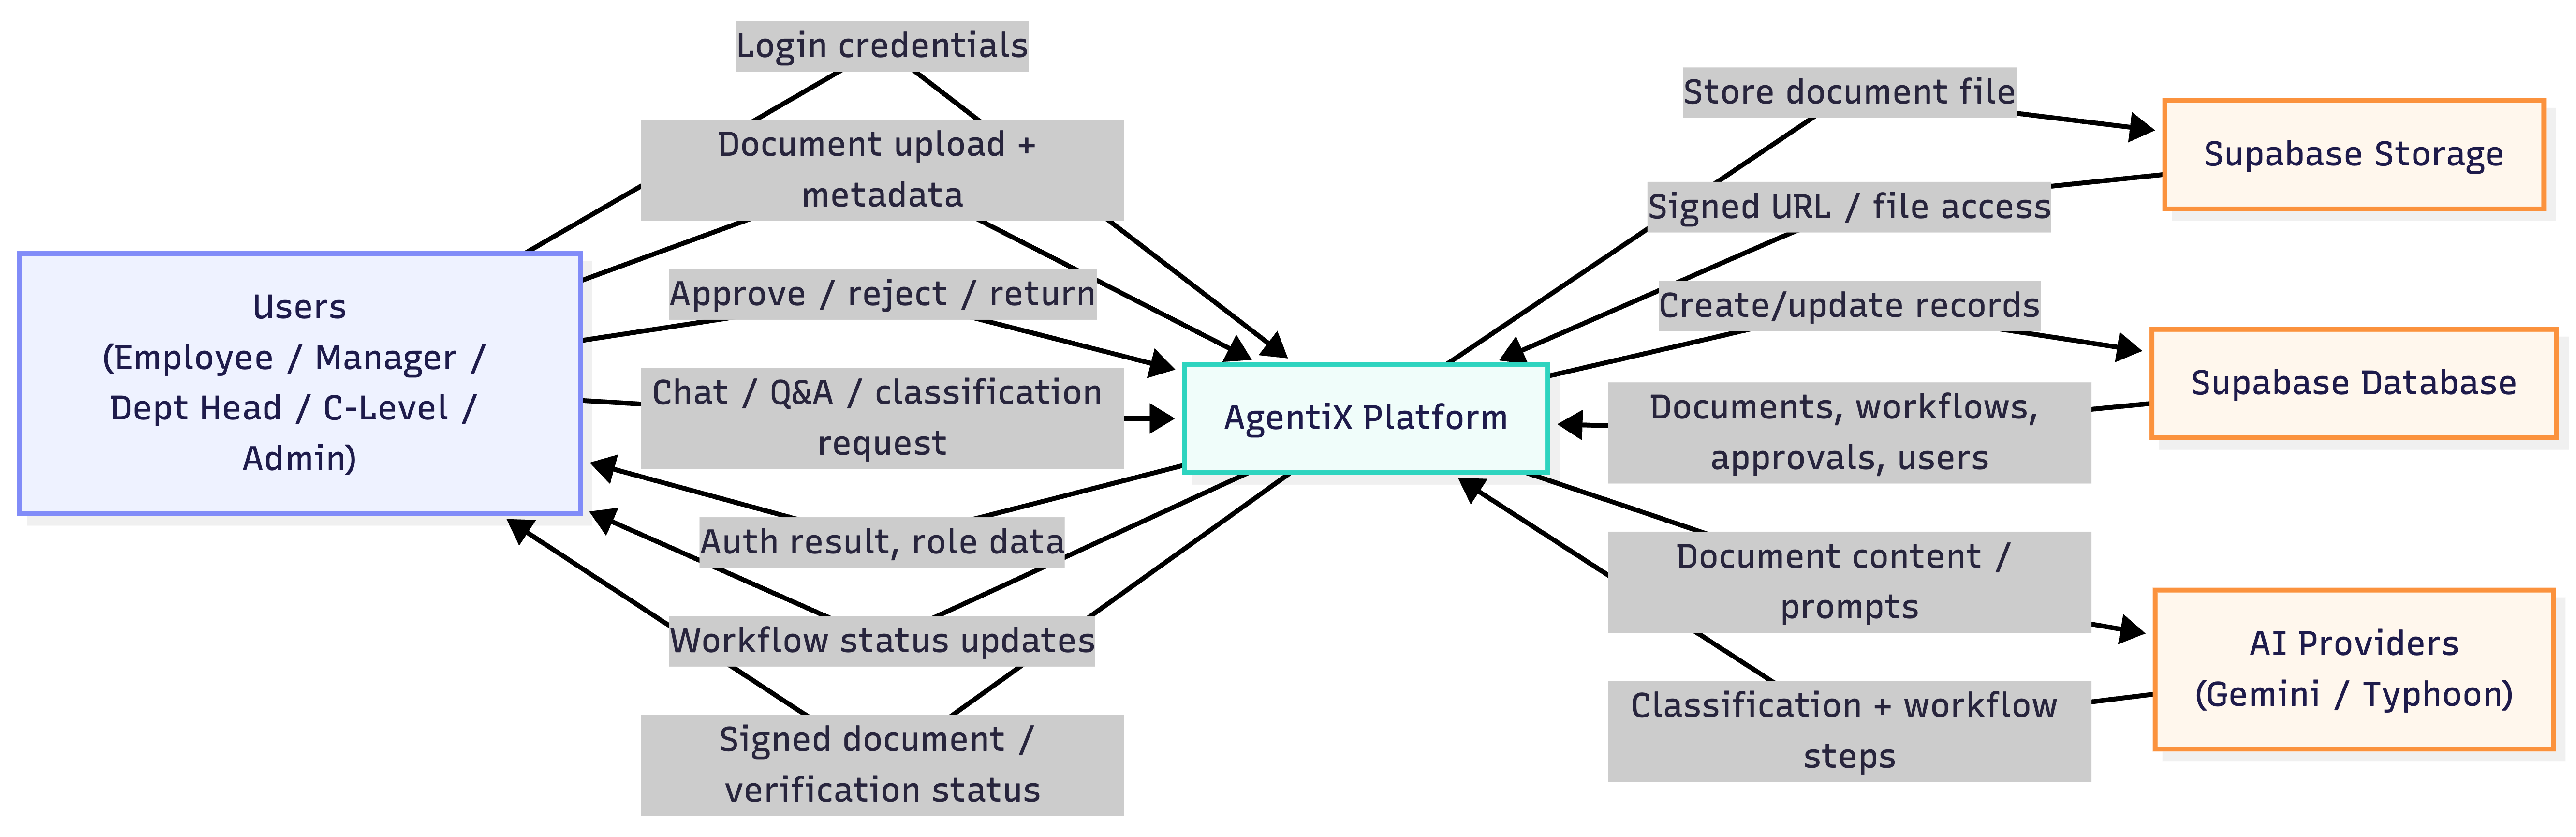
\includegraphics[width=\linewidth]{image/SoftwareDiagram/DFD-L0.png}
\caption{AgentiX DFD Level 0 context diagram.}
\label{fig:dfd-level-0}
\end{figure}

This context-level diagram highlights the AgentiX platform as the central system interacting with external actors and services. Users (employees, managers, department heads, C-level, and admins) submit documents and credentials to the platform, which coordinates storage (Supabase Storage), persistent records (Supabase Database), and external AI providers for classification and workflow generation. The diagram clarifies the high-level boundaries and primary data exchanges that define the system's scope.

At this level the emphasis is on system responsibilities rather than implementation detail: authentication flows, document storage and retrieval, AI-assisted classification, workflow lifecycle, and signature verification are shown as the core capabilities the platform exposes to users and external services.

\subsubsection{DFD Level 1}

\begin{figure}[htbp]
\centering
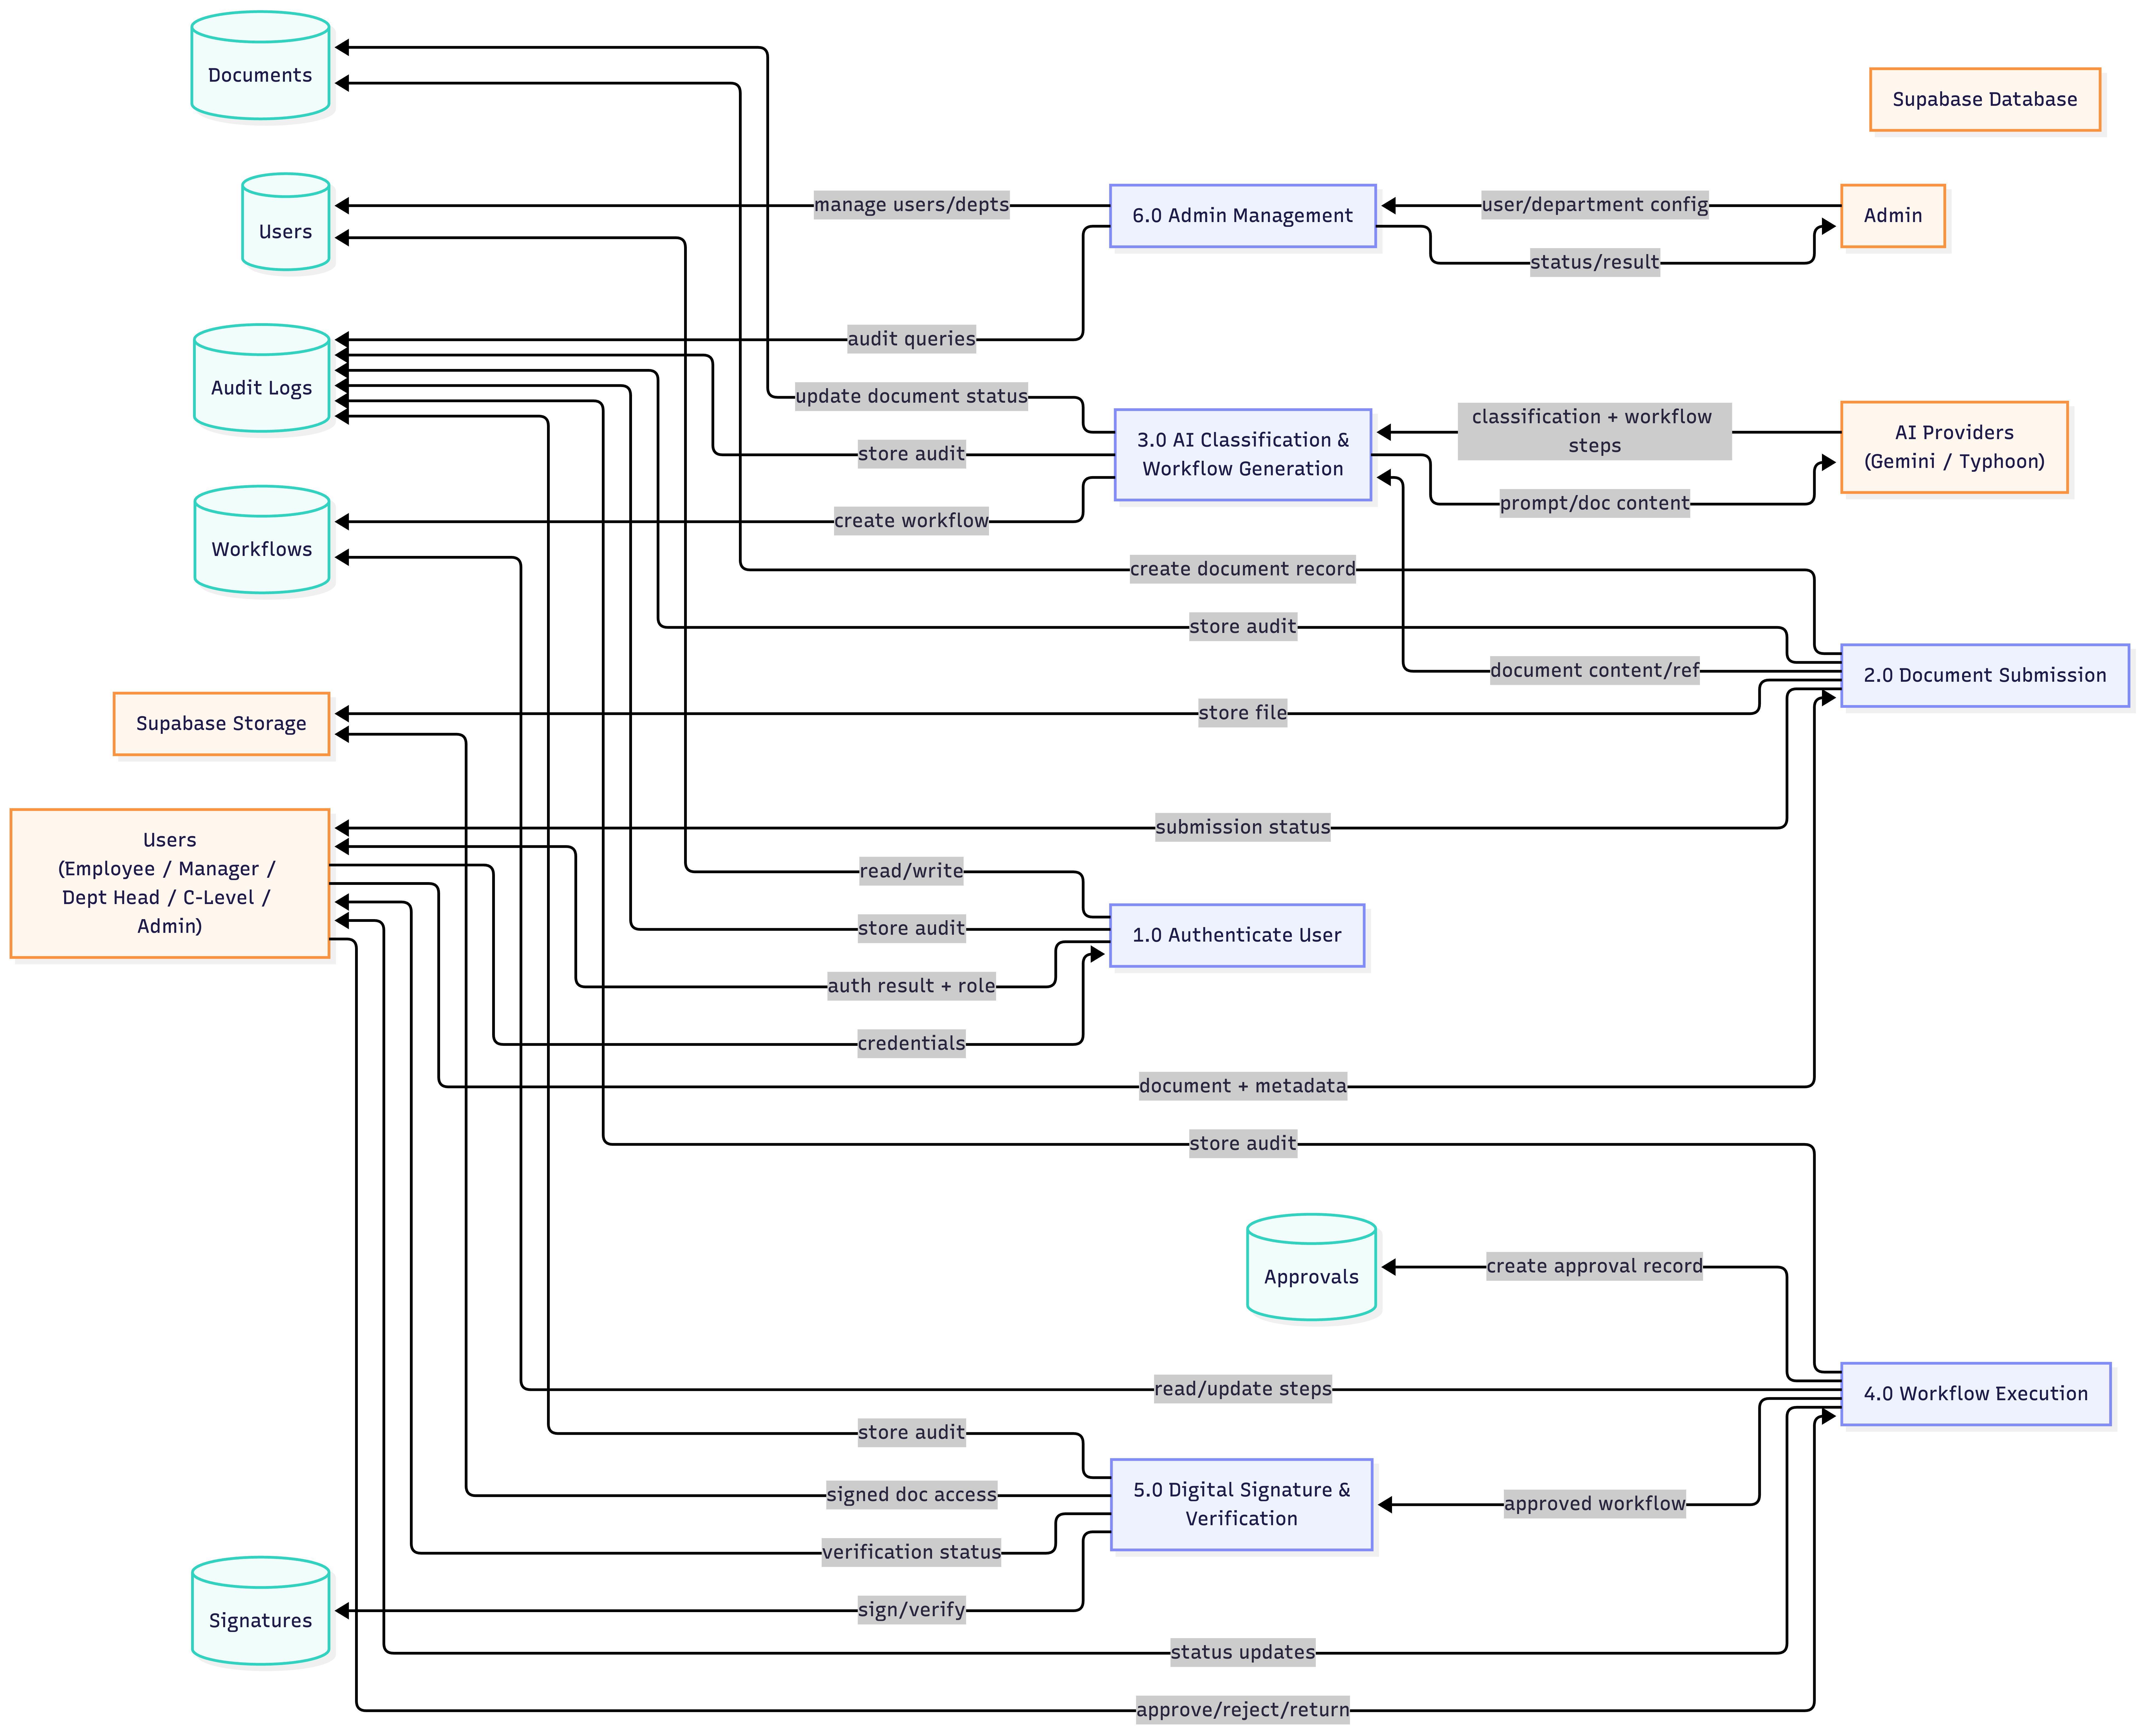
\includegraphics[width=\linewidth]{image/SoftwareDiagram/DFD-L1.png}
\caption{AgentiX DFD Level 1 process decomposition.}
\label{fig:dfd-level-1}
\end{figure}

The Level 1 decomposition expands the context into six primary processes: authentication, document submission, AI classification and workflow generation, workflow execution, digital signature and verification, and admin management. Each process shows the principal data stores (Users, Documents, Workflows, Approvals, Signatures, and Audit Logs) and how they participate in the document lifecycle from submission through archival.

This view is useful for tracing end-to-end responsibilities and for identifying integration touchpoints. It makes explicit where audit logging, persistent state, and external tools (AI providers, storage) are involved, informing both design decisions and security controls for the platform.

\subsubsection{DFD Level 2}

\begin{figure}[htbp]
\centering
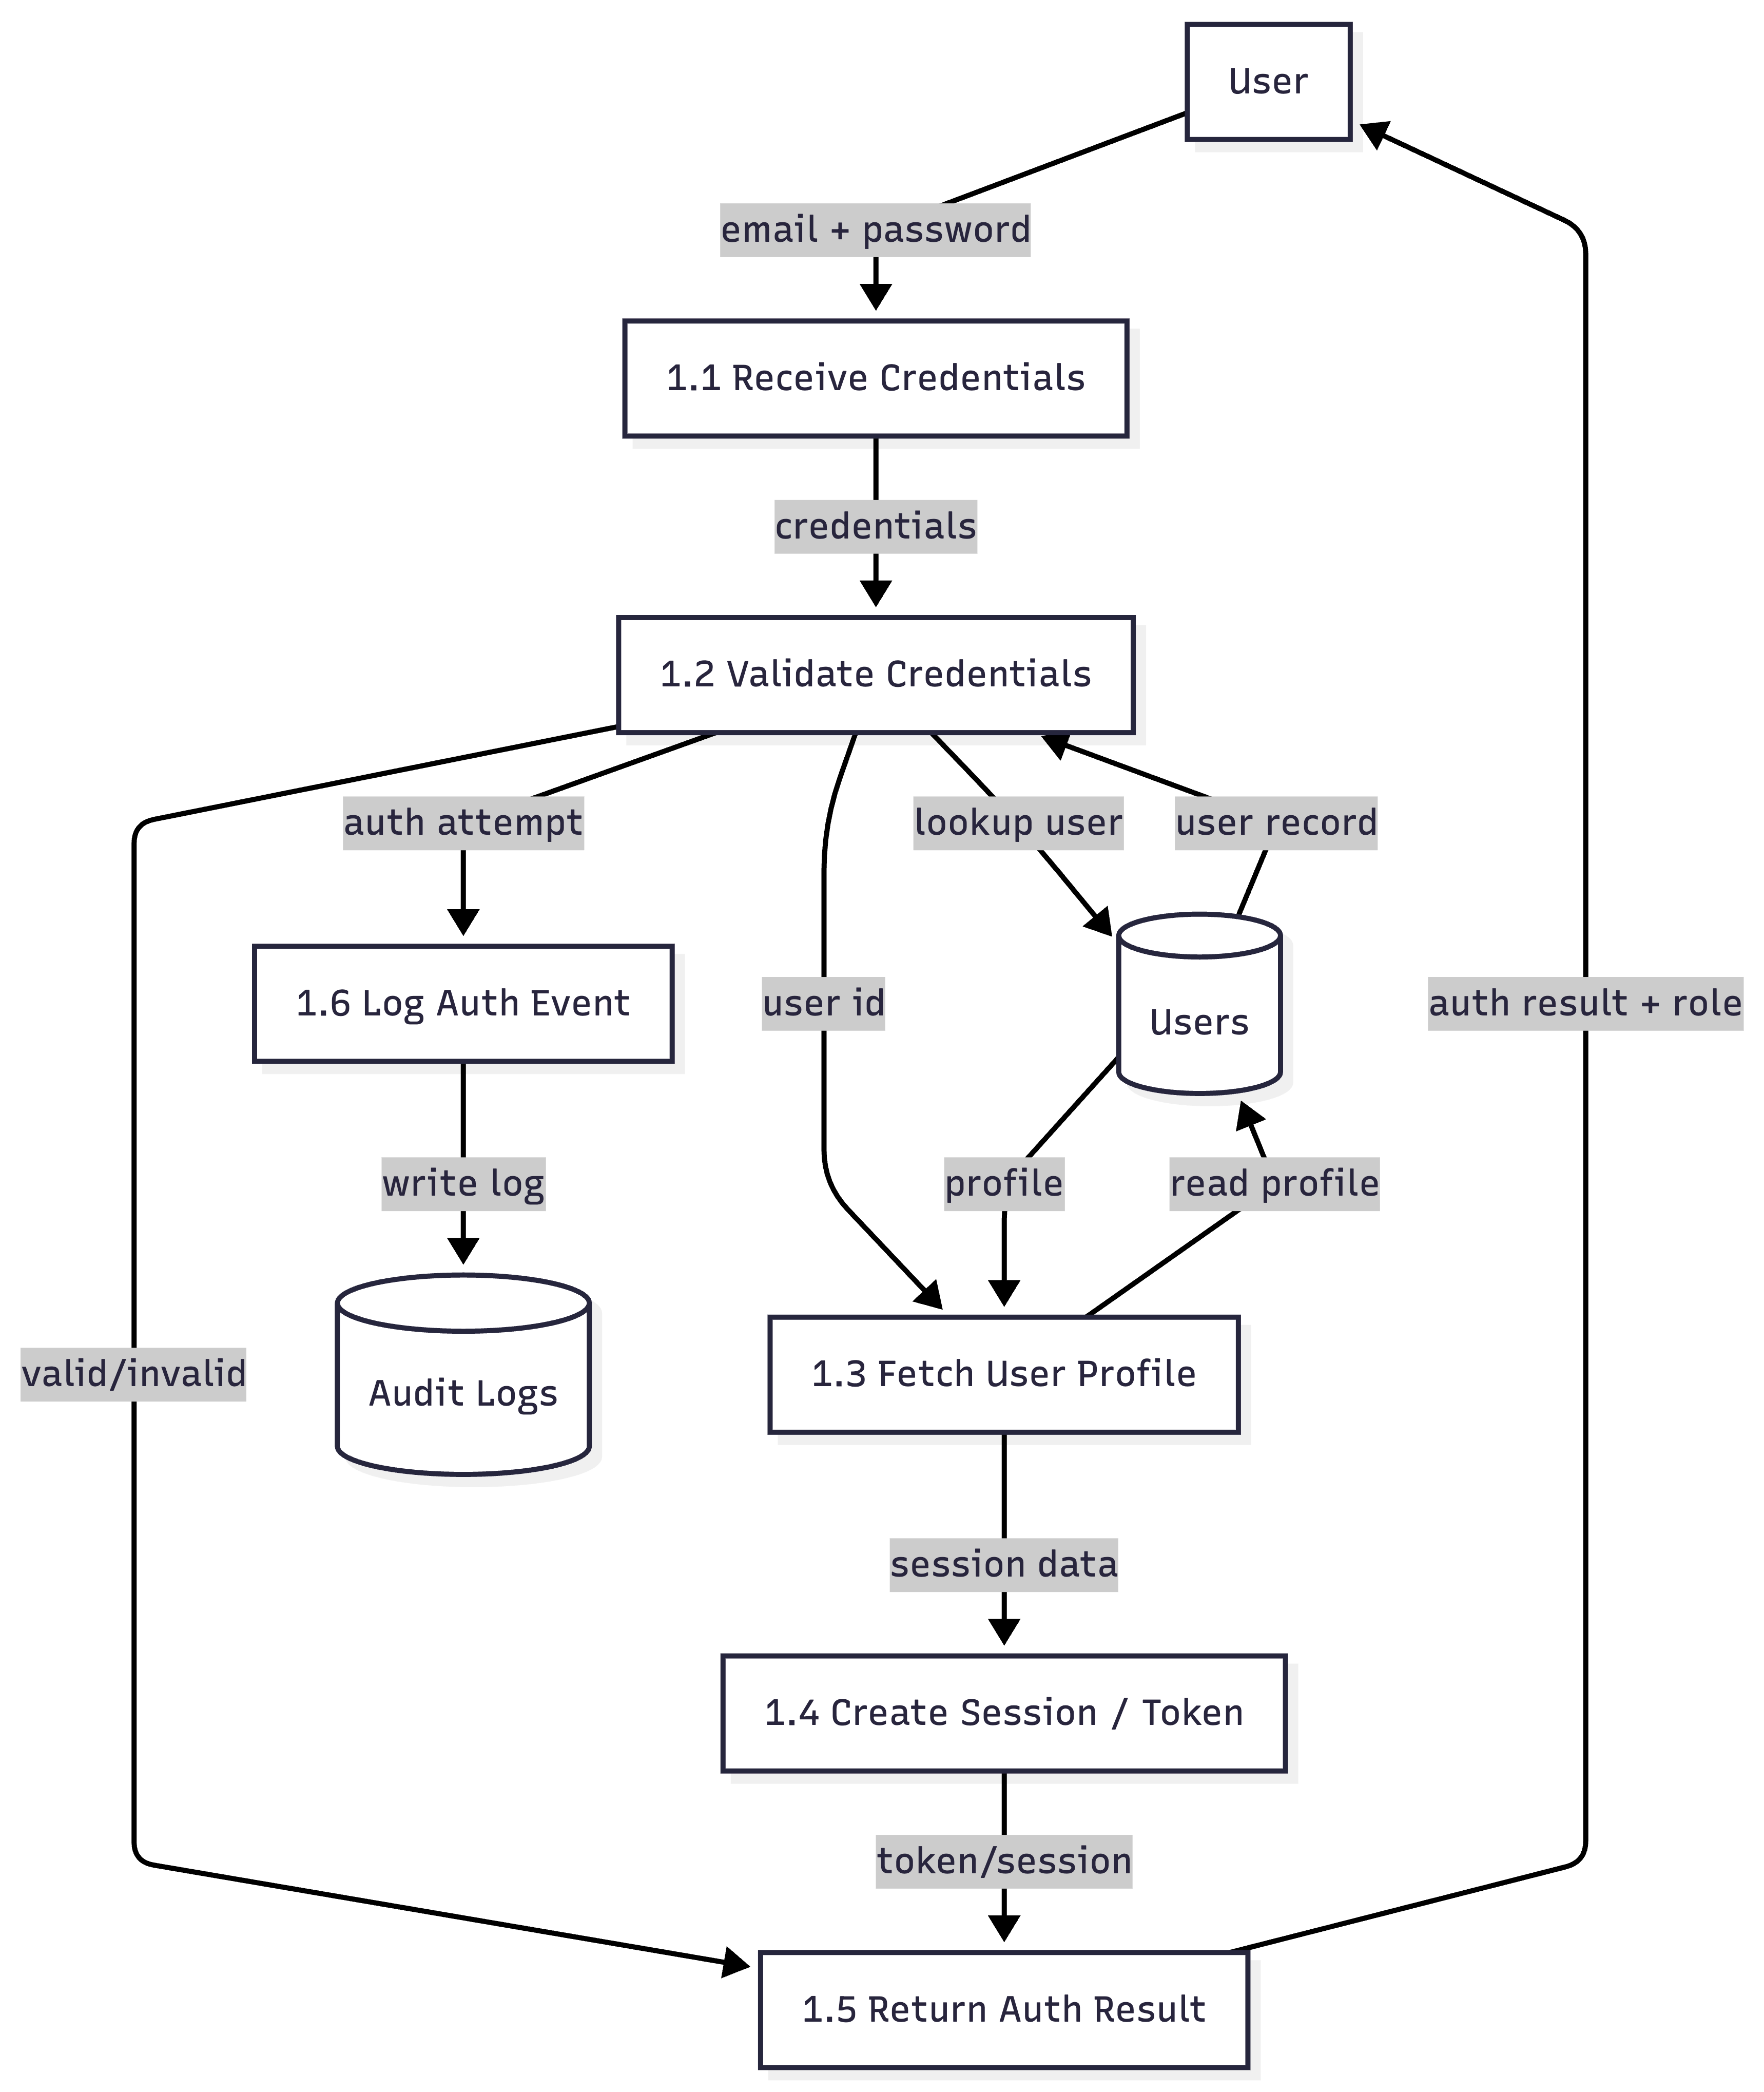
\includegraphics[width=\linewidth]{image/SoftwareDiagram/DFD-L2-P1-AuthenticateUser.png}
\caption{DFD Level 2 for Process 1.0 Authenticate User.}
\label{fig:dfd-level-2-auth}
\end{figure}

The Authenticate User diagram details the credential flow: the system receives user credentials, validates them against the Users data store, and, upon success, fetches profile data and issues a session token. An audit event is recorded for each authentication attempt, ensuring traceability for security investigations and policy enforcement.

This level-2 view clarifies how authentication ties into user profile management and auditing: it shows that credential validation is separate from profile retrieval and that session creation is an explicit operation, which simplifies reasoning about session lifecycle and access control.

\begin{figure}[htbp]
\centering
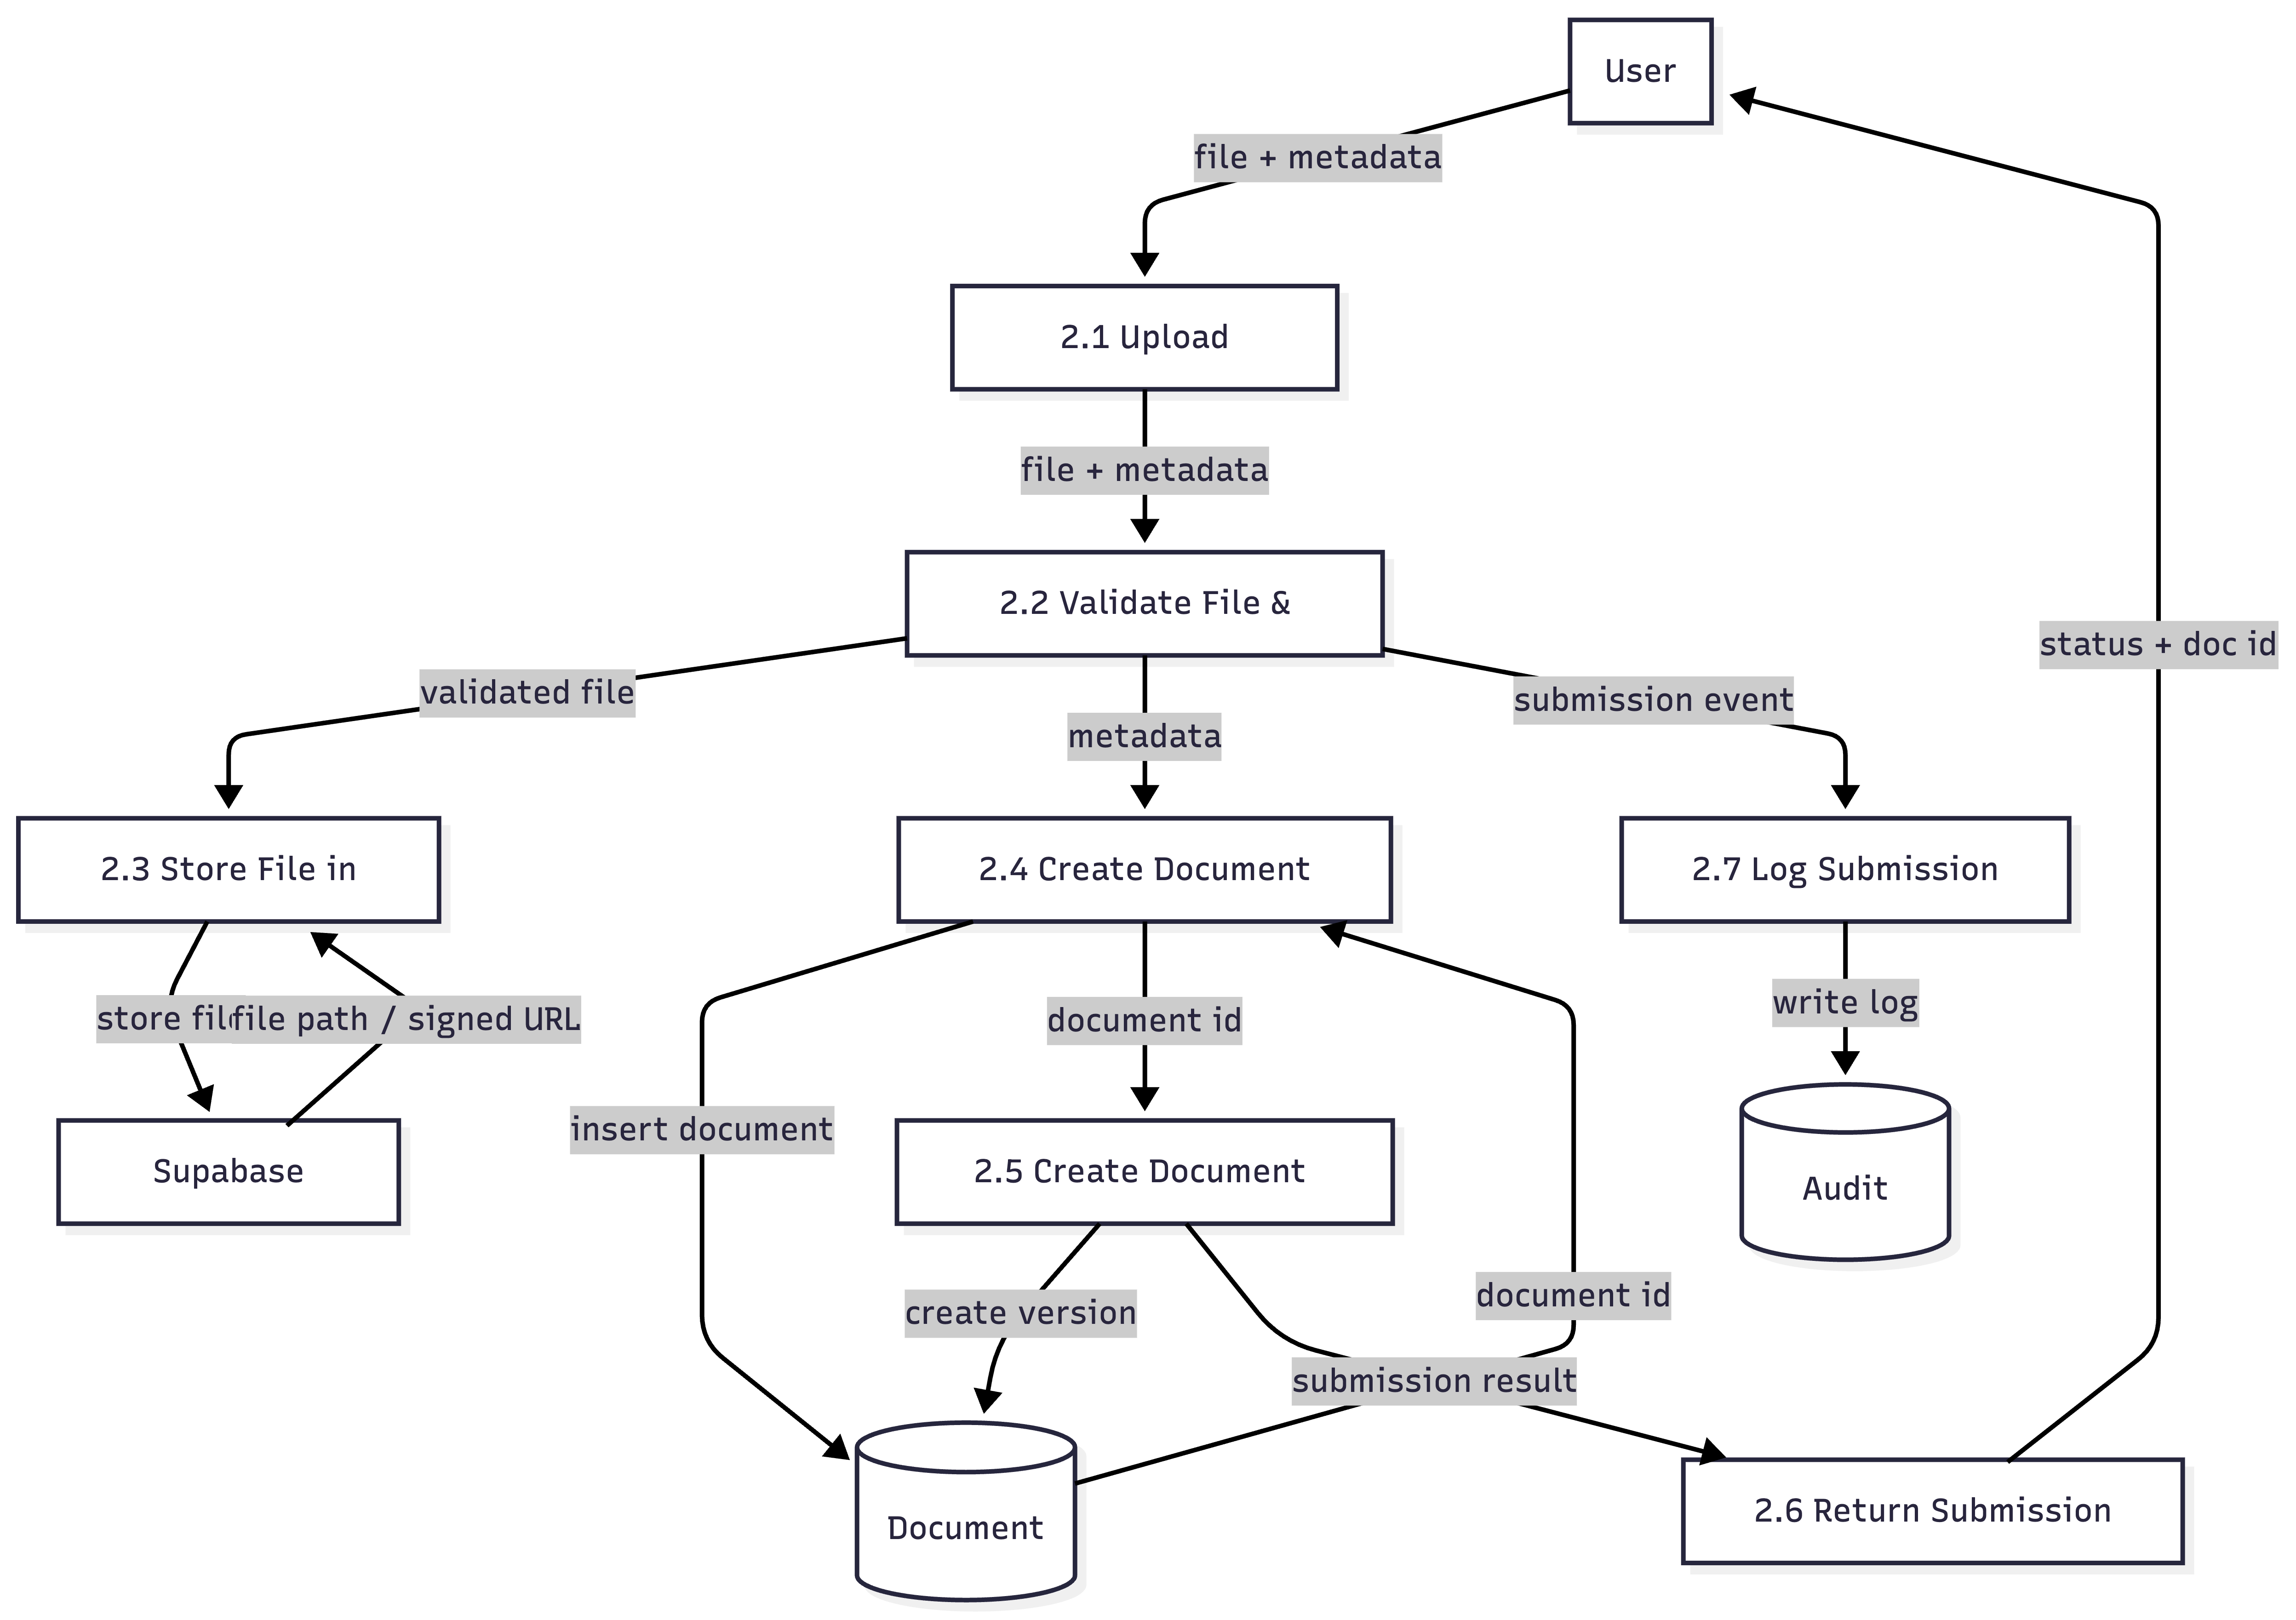
\includegraphics[width=\linewidth]{image/SoftwareDiagram/DFD-L2-P2-DocumentSubmission.png}
\caption{DFD Level 2 for Process 2.0 Document Submission.}
\label{fig:dfd-level-2-submit}
\end{figure}

The Document Submission diagram describes the intake pipeline: users upload files and metadata, which are validated and then stored in object storage (Supabase). A document record is created in the Documents datastore and versioning information is recorded. Submission events are logged to the audit store to support traceability and troubleshooting.

This decomposition separates file-level concerns (storage, signed URLs) from metadata and record management, making it clear where virus scanning, format normalization, and metadata validation should be implemented within the intake worker.

\begin{figure}[htbp]
\centering
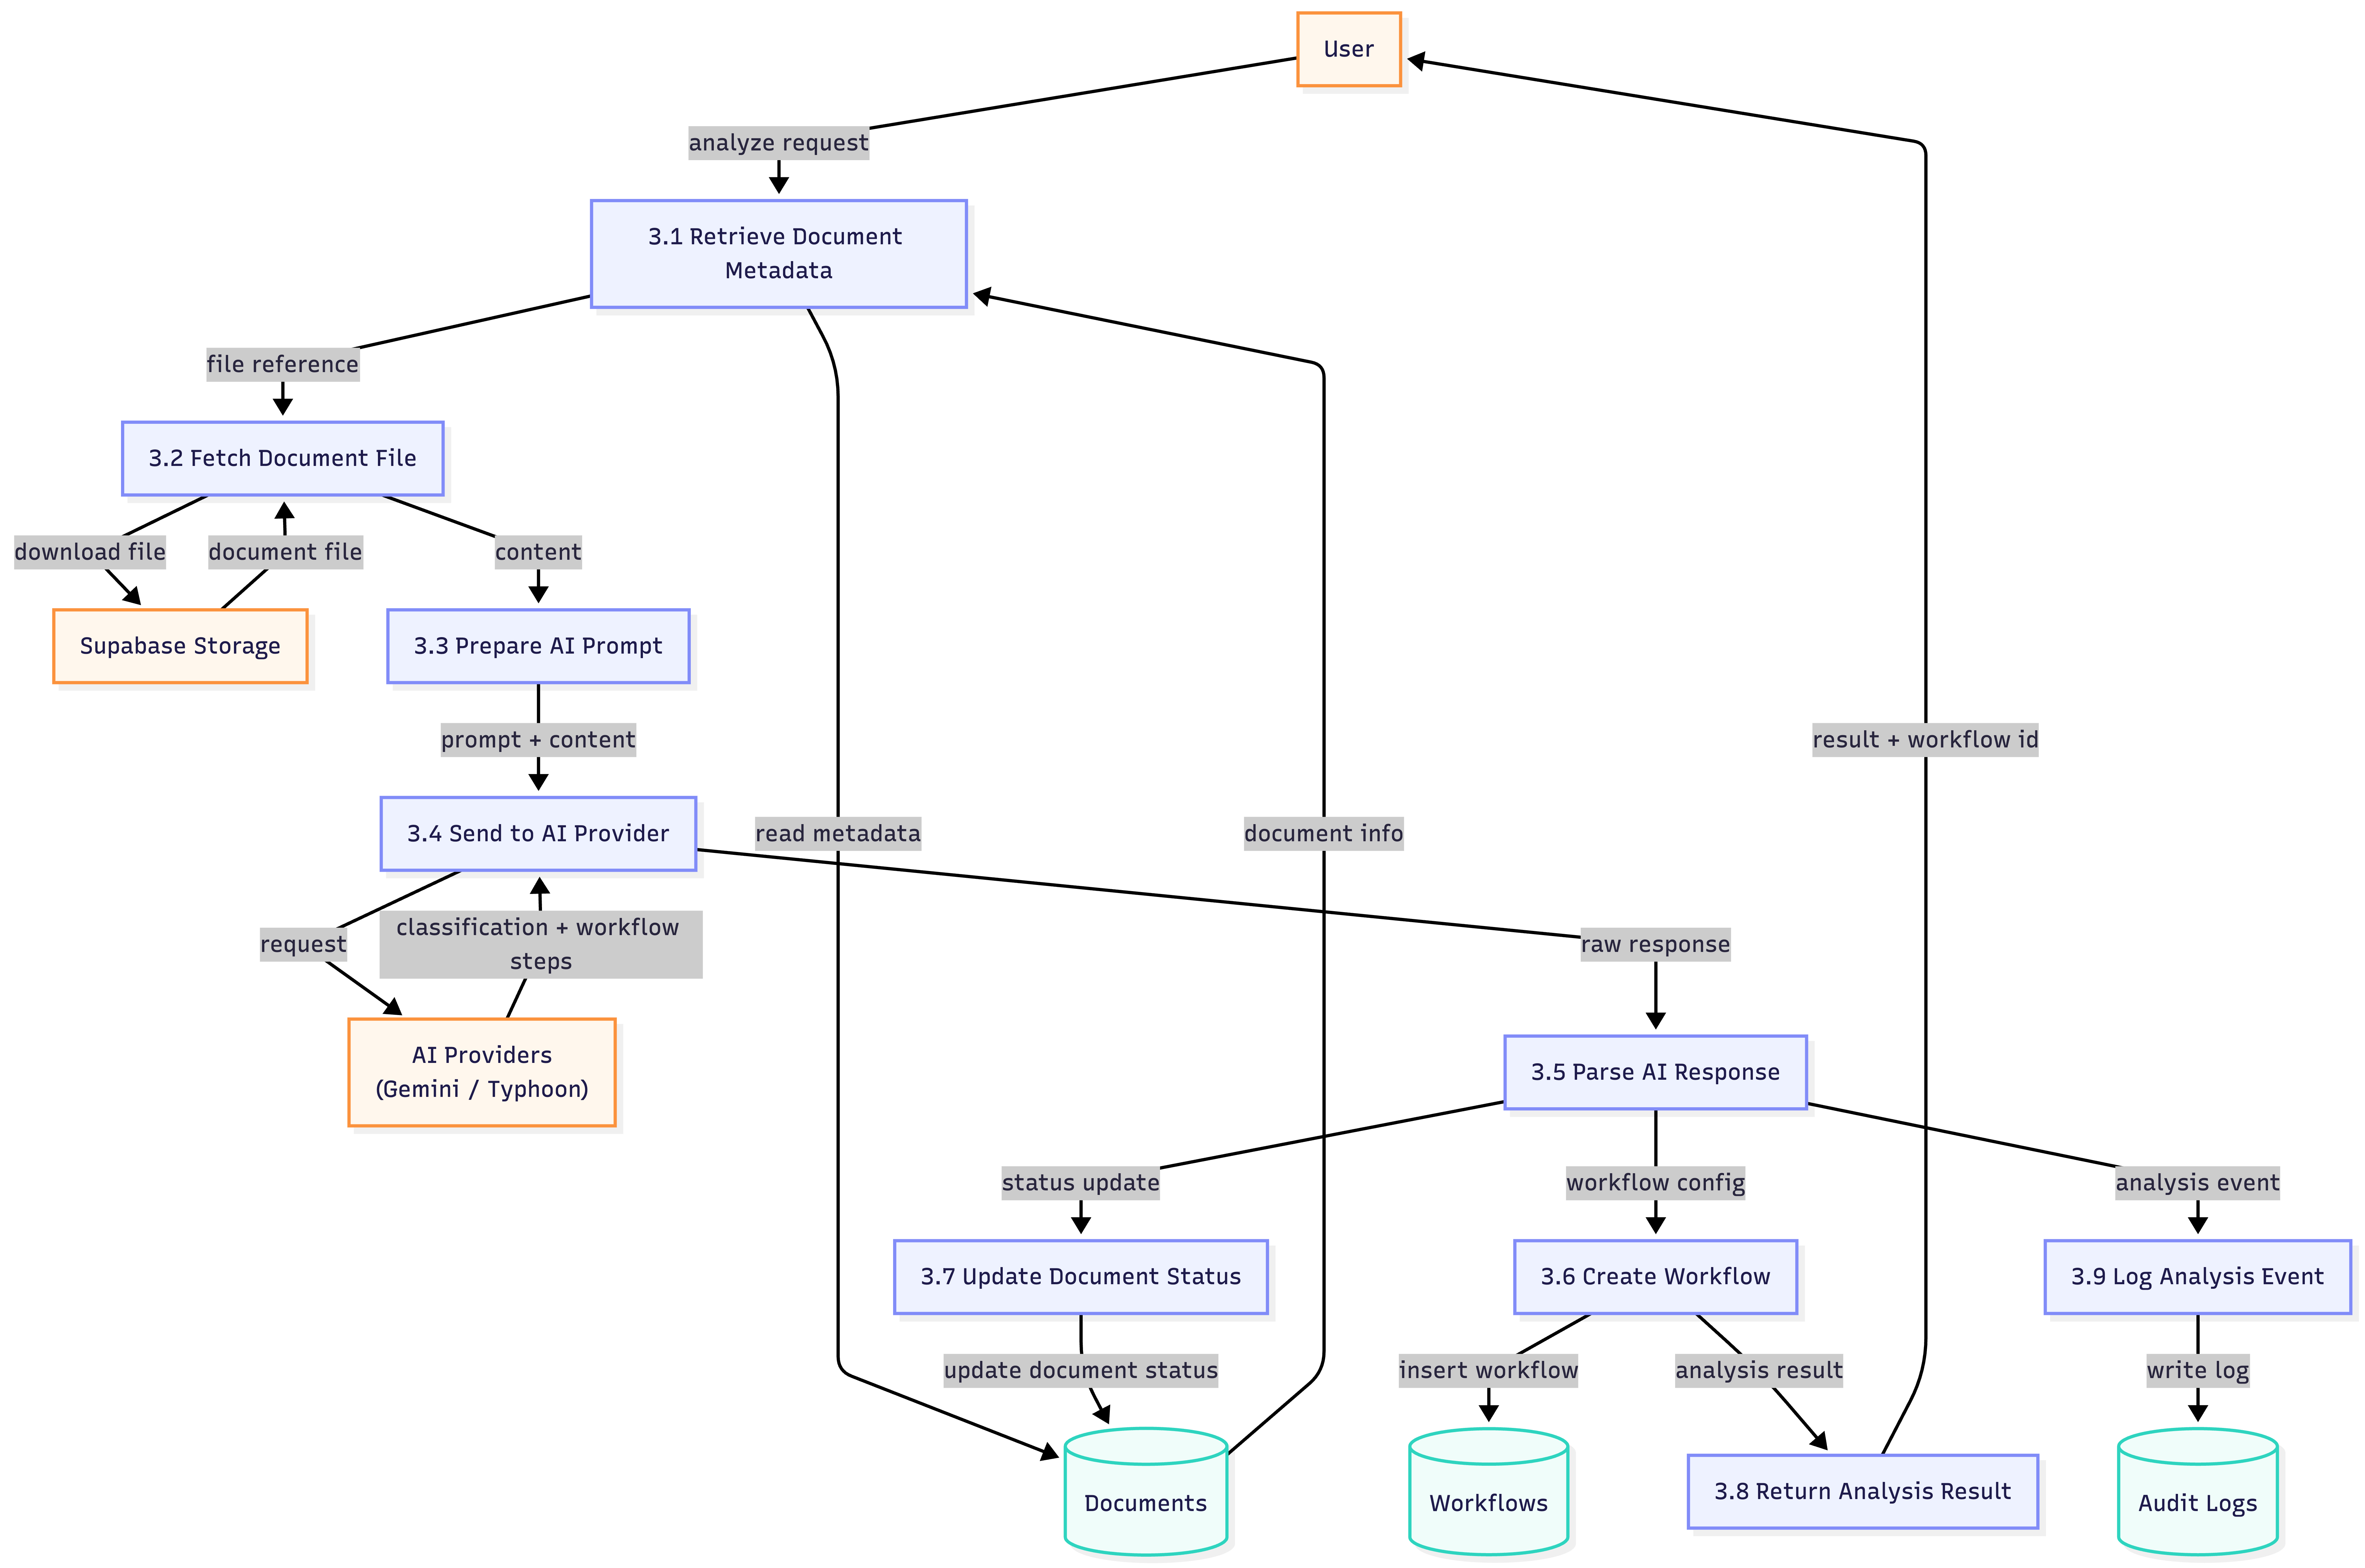
\includegraphics[width=\linewidth]{image/SoftwareDiagram/DFD-L2-P3-Classification+WorkflowGen.png}
\caption{DFD Level 2 for Process 3.0 AI Classification and Workflow Generation.}
\label{fig:dfd-level-2-classify}
\end{figure}

The AI Classification and Workflow Generation diagram shows how document metadata and content are fetched, converted into an AI prompt, and sent to external AI providers (e.g., Gemini or Typhoon). The AI's response is parsed and transformed into a workflow configuration which is persisted into the Workflows datastore; the document status is updated and an analysis event is logged.

This flow emphasises the separation between data retrieval, AI invocation, and post-processing. It highlights the need for prompt preparation, response parsing, and validation steps to ensure that automatically generated workflows meet policy constraints before being enacted.

\begin{figure}[htbp]
\centering
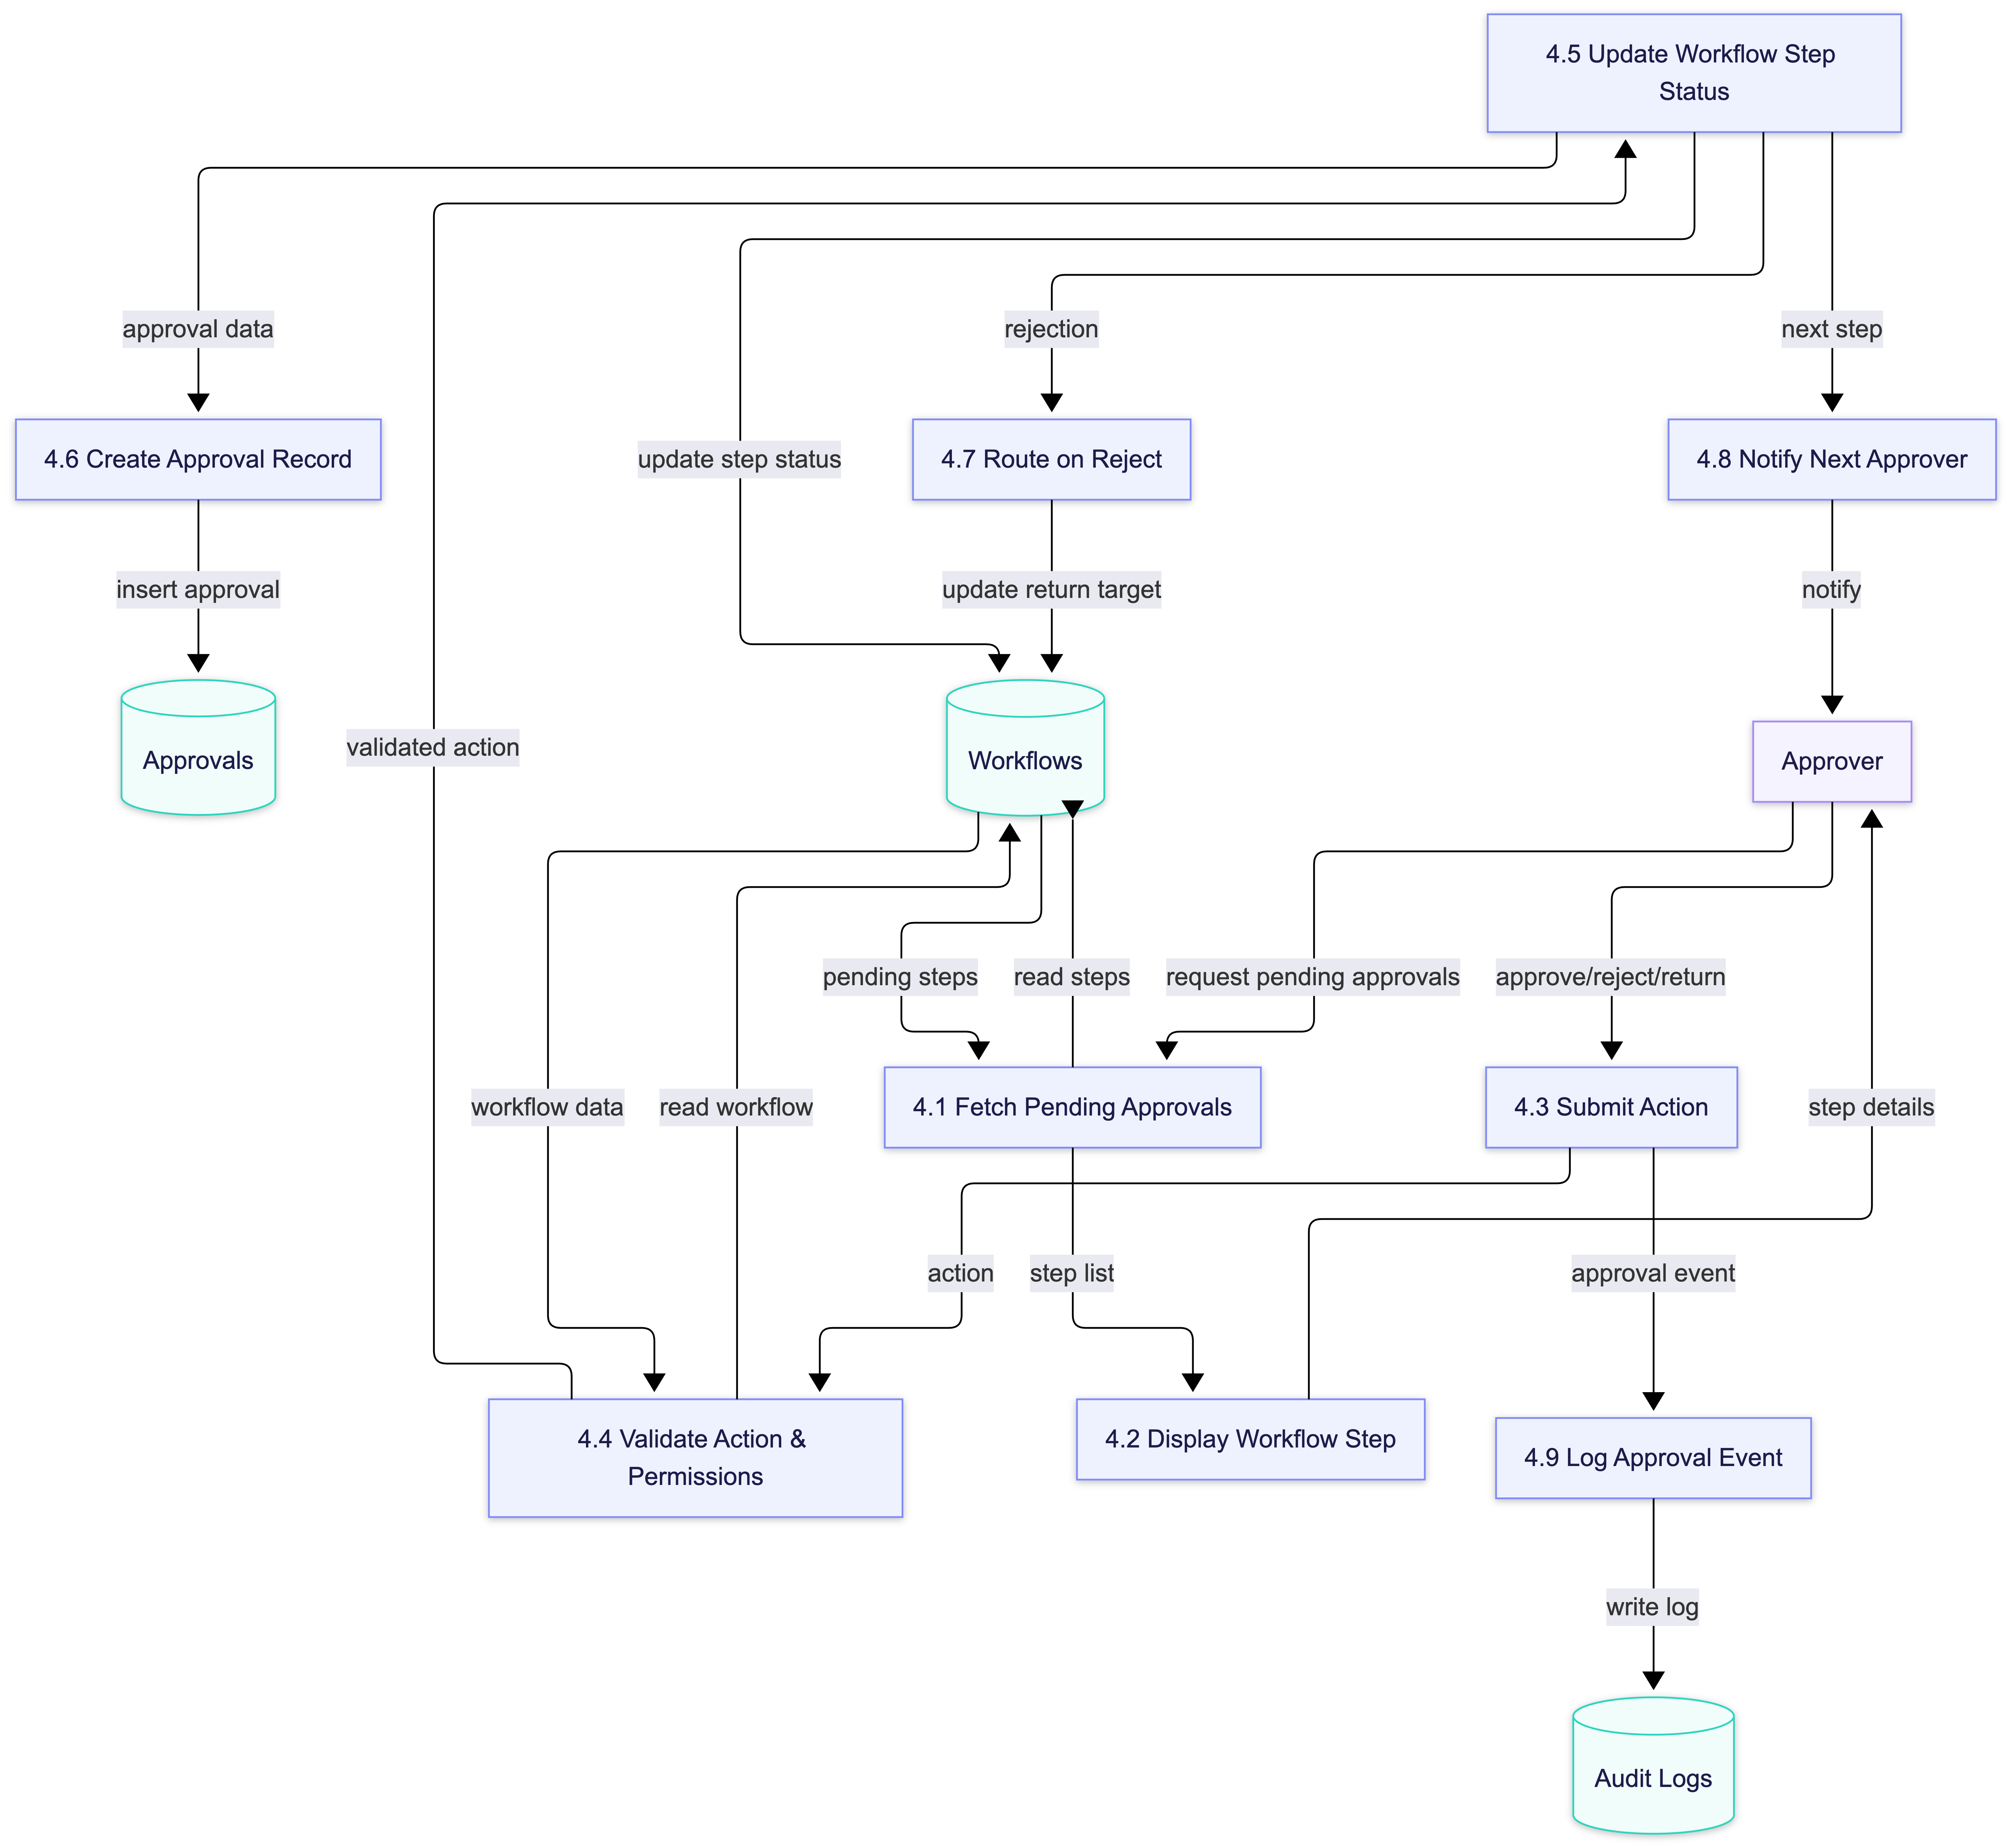
\includegraphics[width=\linewidth]{image/SoftwareDiagram/DFD-L2-P4-WorkflowExecution.png}
\caption{DFD Level 2 for Process 4.0 Workflow Execution.}
\label{fig:dfd-level-2-workflow}
\end{figure}

Workflow Execution covers the runtime interaction between approvers and the orchestration engine: pending steps are retrieved from the Workflows store, displayed to users, and actor actions (approve, reject, return) are validated against permissions. Actions update workflow state and create approval records, and reject or return events trigger routing adjustments and notifications to the next approver.

This diagram makes explicit the operational responsibilities—permission checks, step state transitions, approval records, and notification logic—so designers can ensure proper concurrency handling, SLA enforcement, and reliable notification delivery.

\begin{figure}[htbp]
\centering
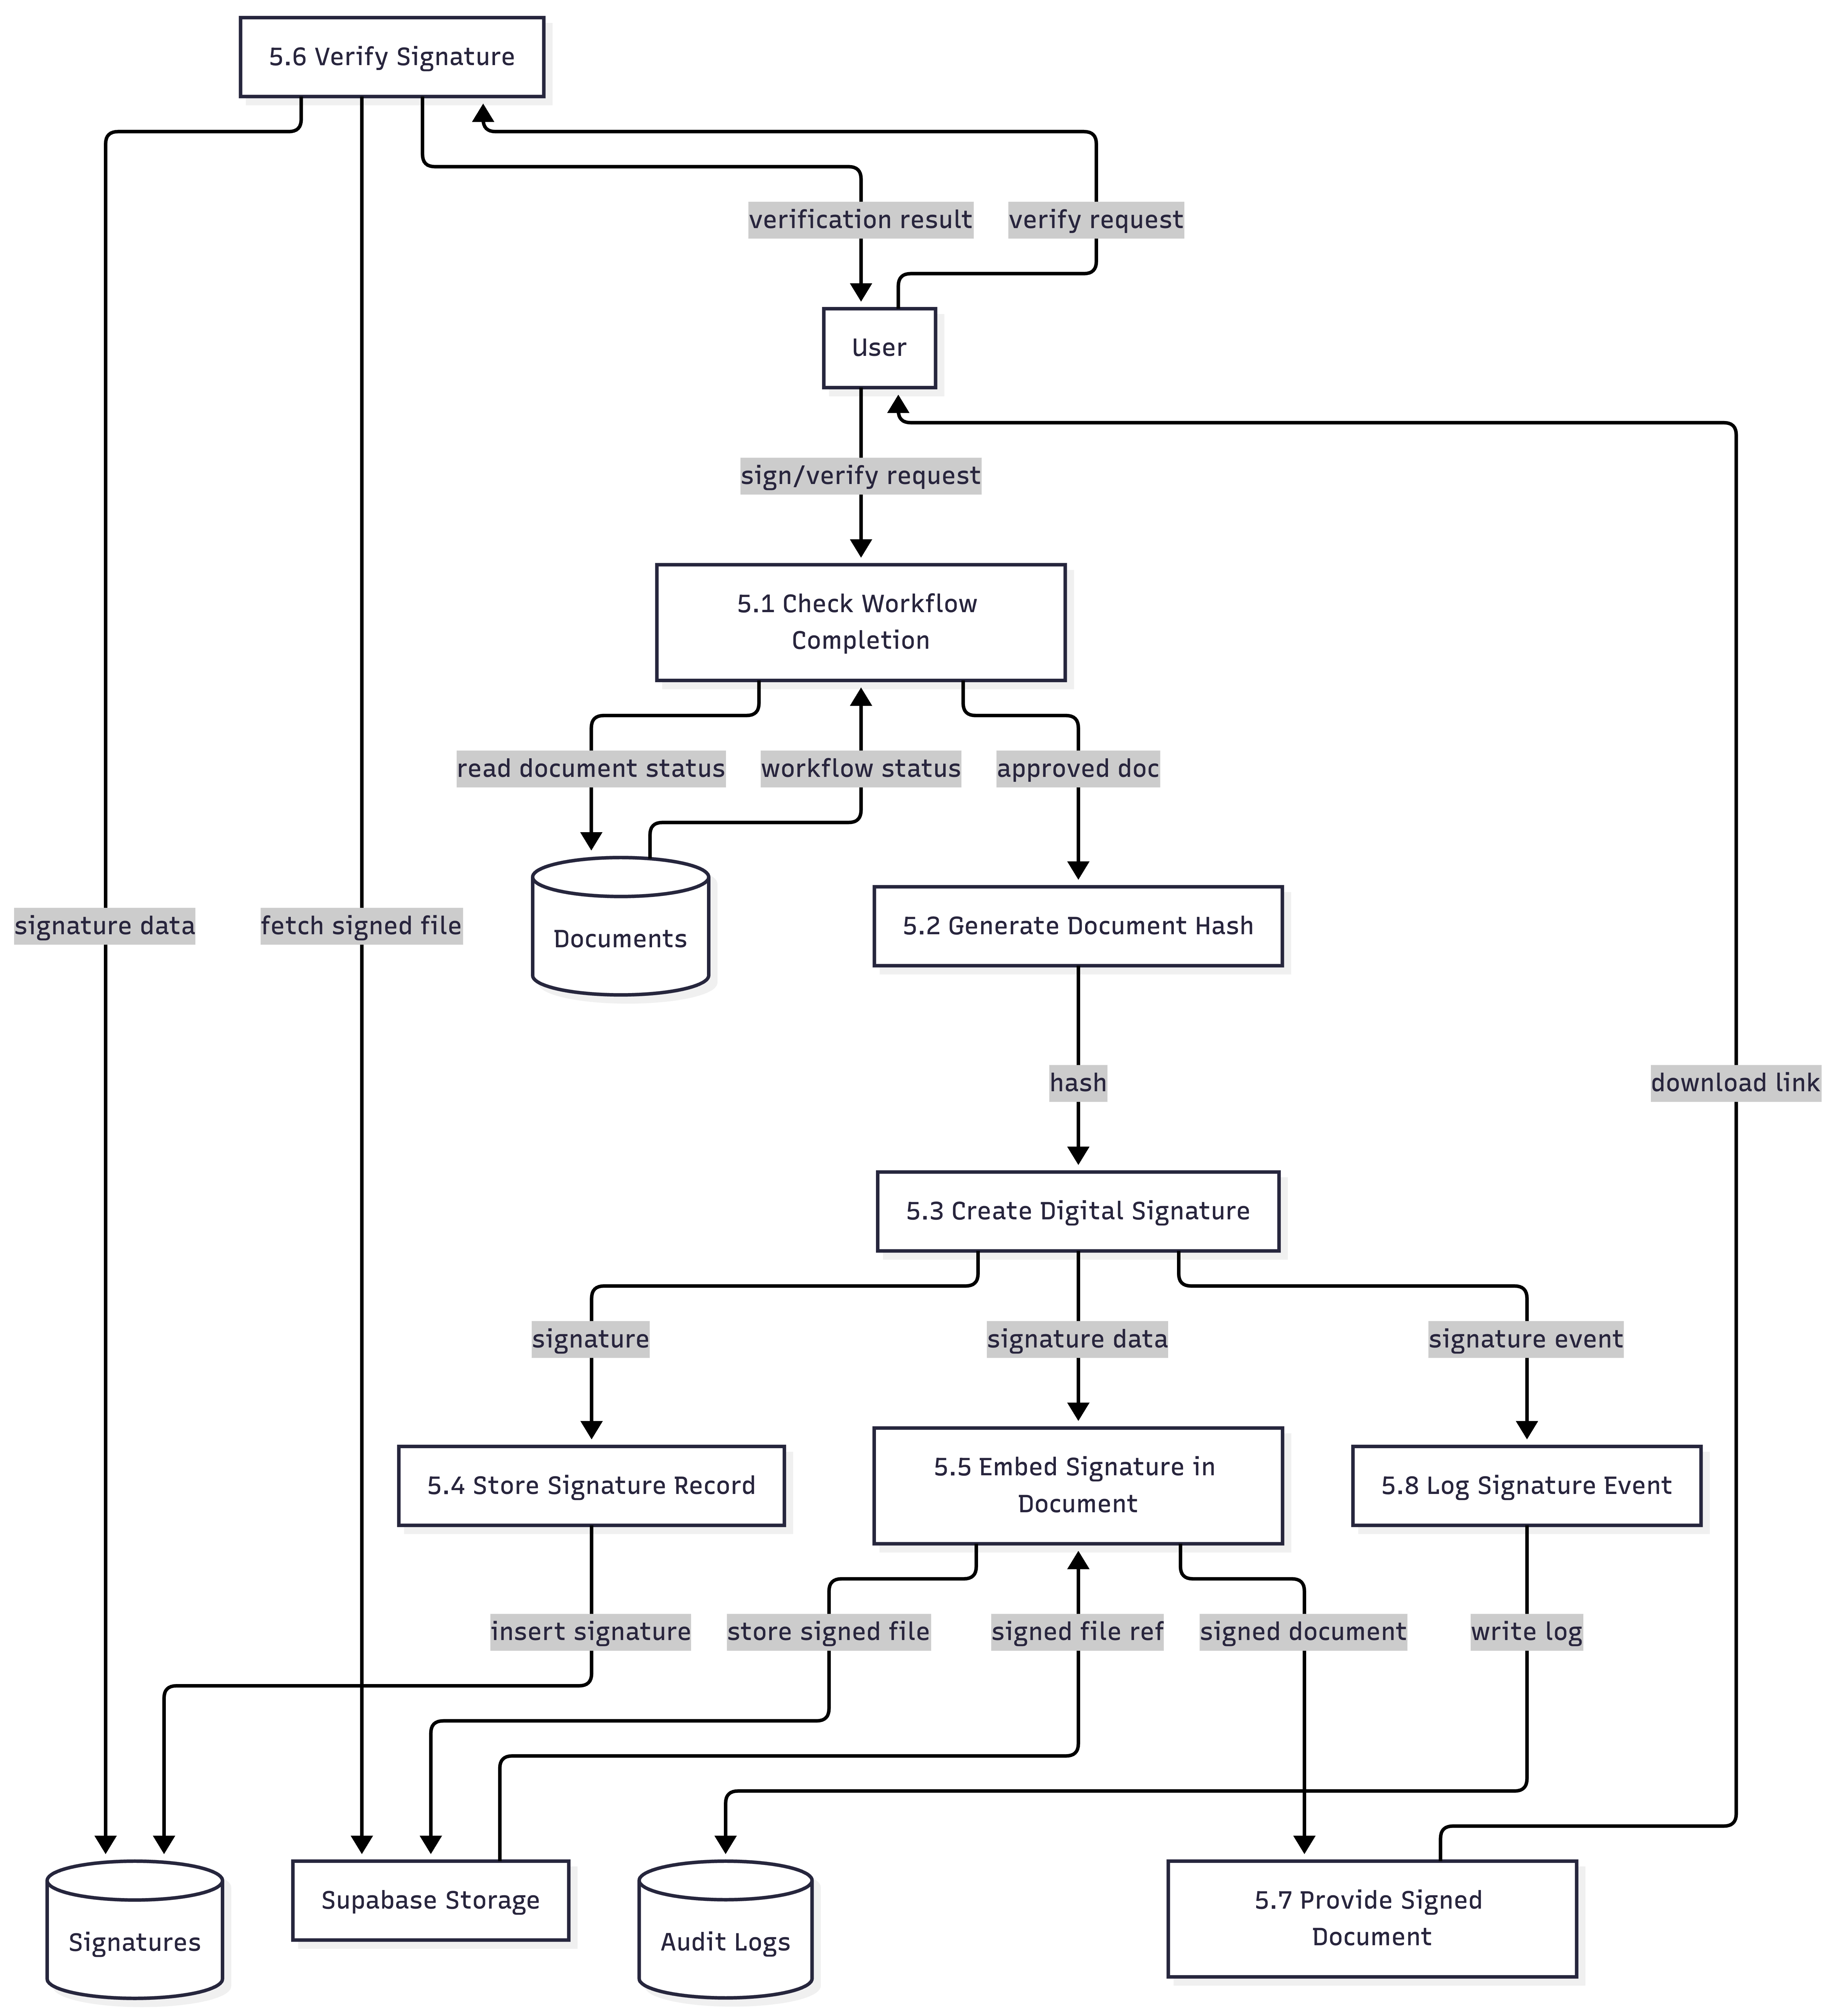
\includegraphics[width=\linewidth]{image/SoftwareDiagram/DFD-L2-P5-DigitalSignature+Verification.png}
\caption{DFD Level 2 for Process 5.0 Digital Signature and Verification.}
\label{fig:dfd-level-2-signature}
\end{figure}

The Digital Signature and Verification diagram outlines the signing lifecycle: once a workflow is complete, the system generates a document hash, creates a digital signature, stores the signature record, and embeds the signature into the document stored in object storage. Verification requests retrieve the signed file and signature record to confirm integrity and authenticity, with signature events recorded in the audit log.

This view clarifies how signature generation, evidence storage, and verification interact with the broader system, and highlights the places where HSM/TSA/OCSP integrations and long-term validation (LTV) should be applied to meet compliance requirements.

\begin{figure}[htbp]
\centering
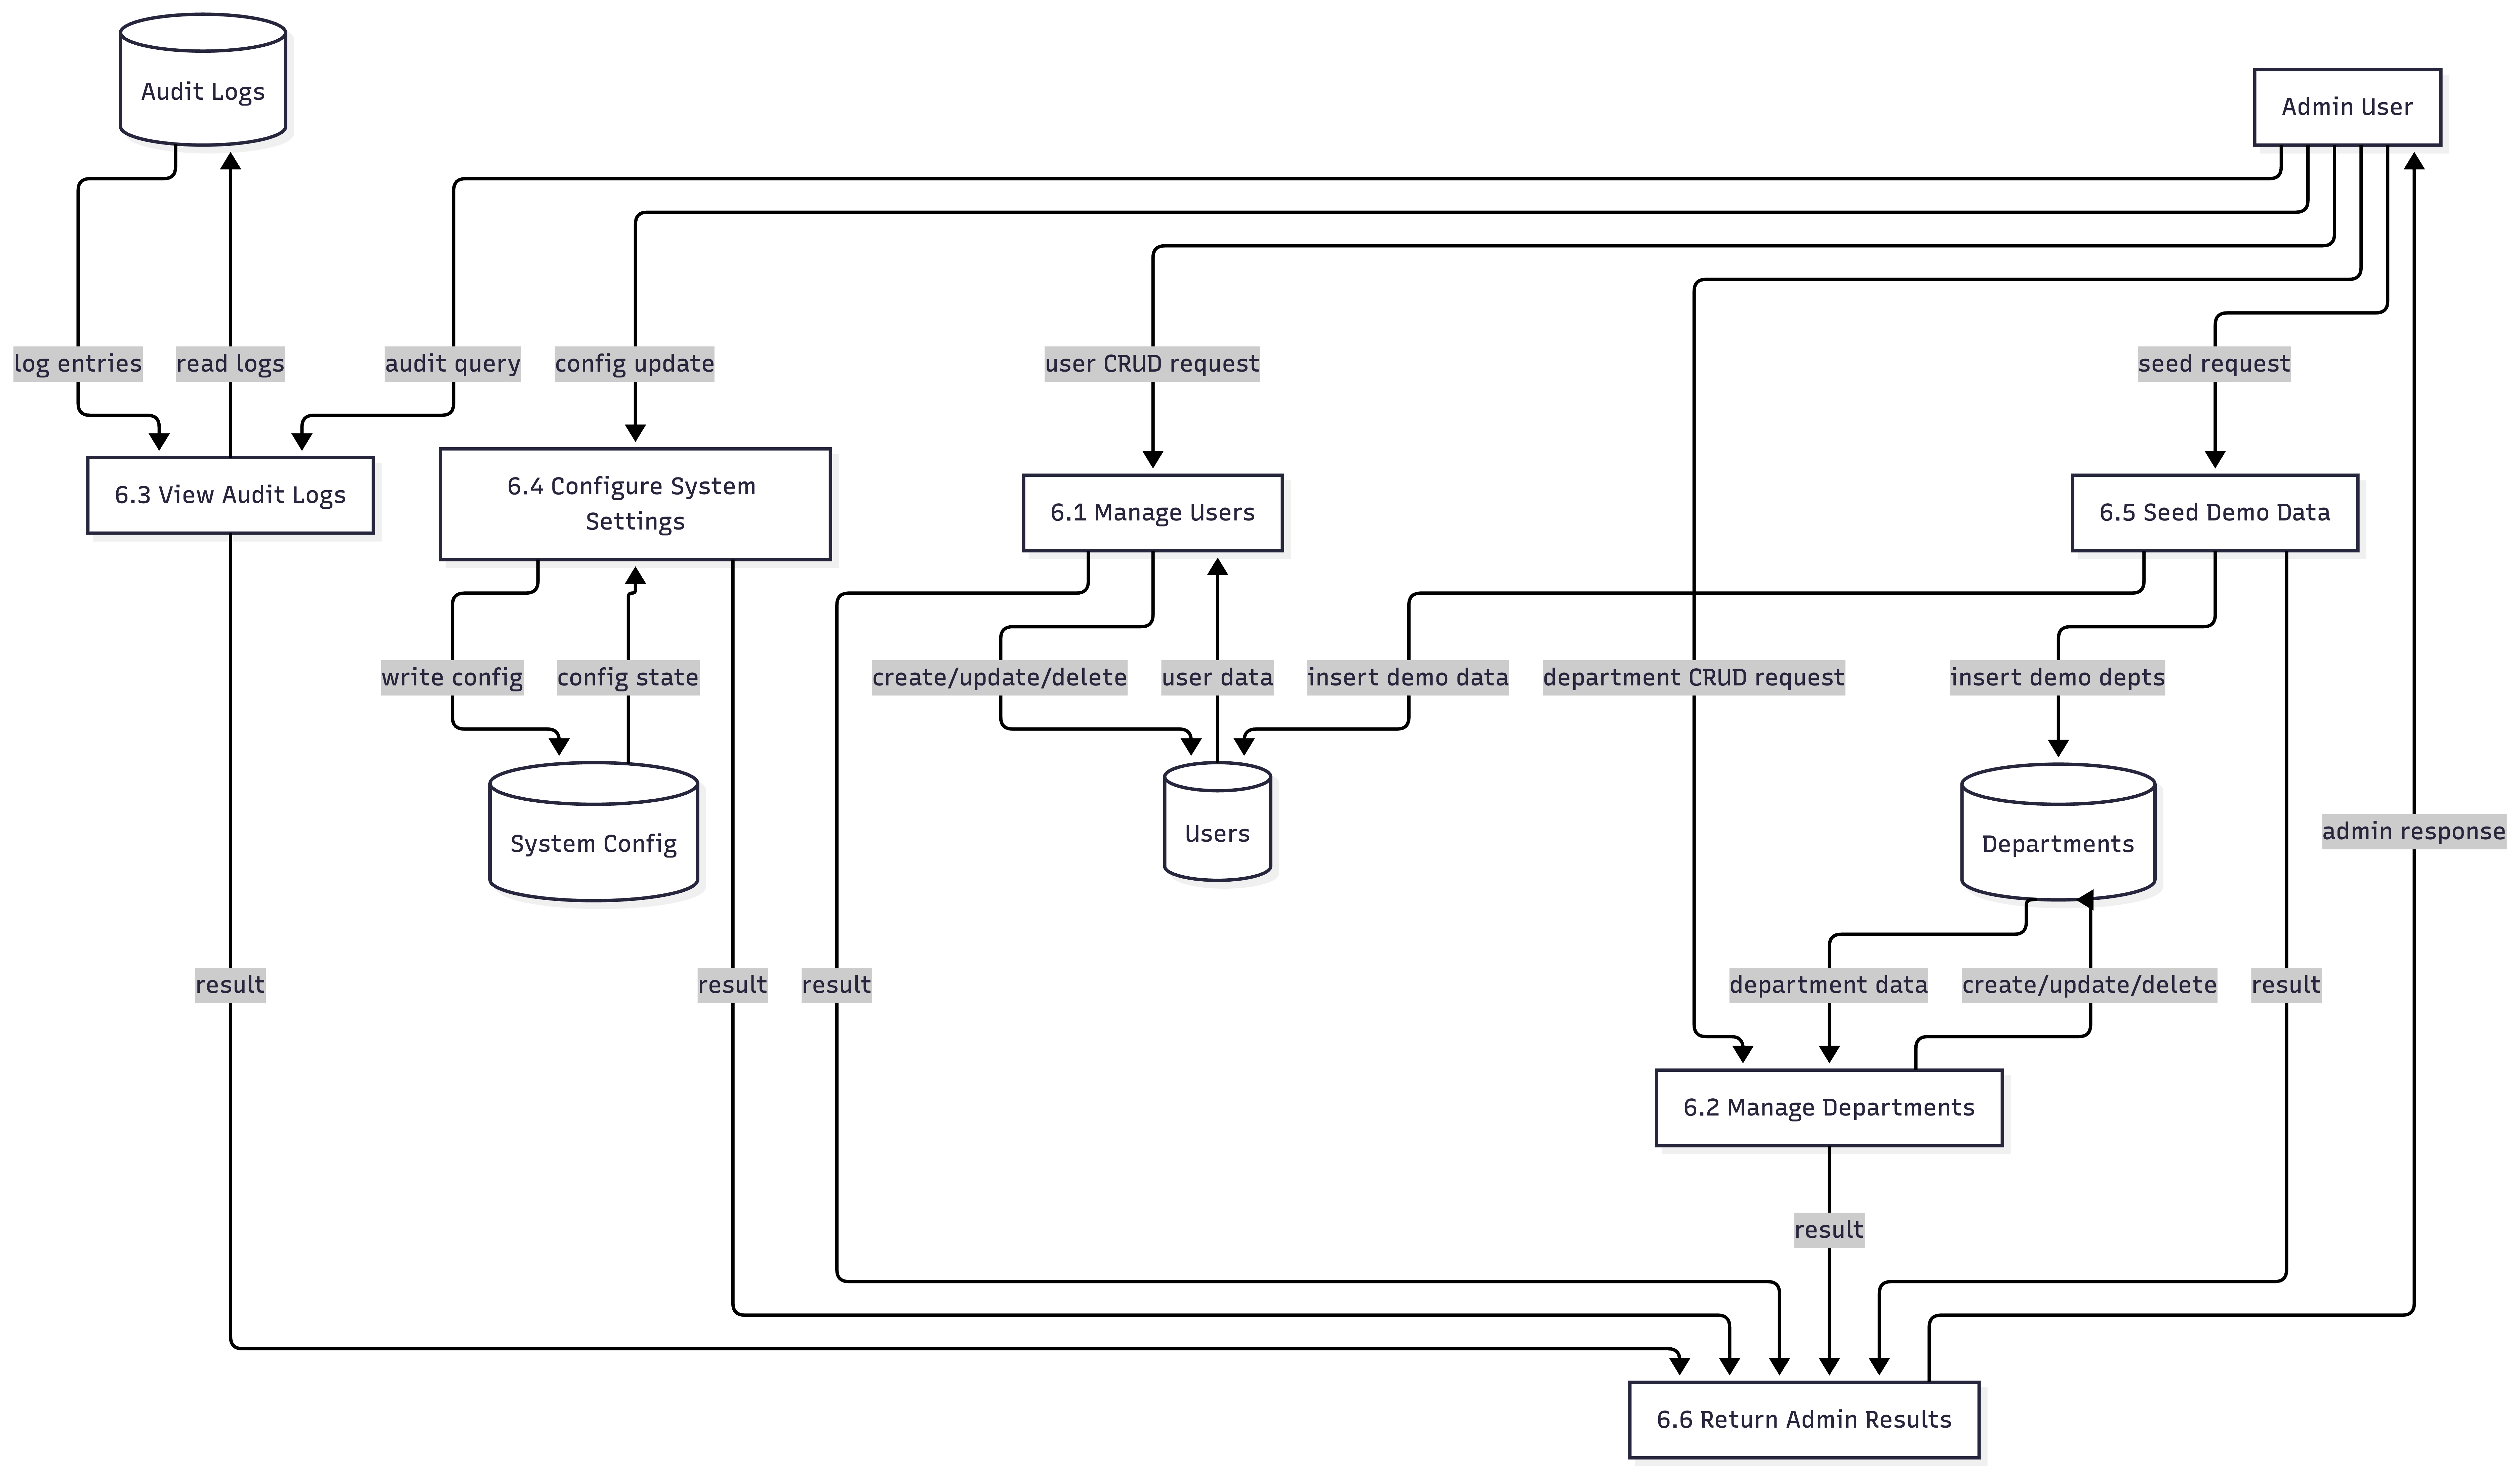
\includegraphics[width=\linewidth]{image/SoftwareDiagram/DFD-L2-P6-AdminManagement.png}
\caption{DFD Level 2 for Process 6.0 Admin Management.}
\label{fig:dfd-level-2-admin}
\end{figure}

Admin Management shows the administrative operations: user and department CRUD, audit log queries, system configuration updates, and seeding demo data. Each administrative action updates the corresponding datastore and funnels results back to the admin interface, with admin operations consolidated through a return/results node for consistent feedback.

This diagram underscores administrative responsibilities and the need for hardened access controls, auditability, and safe defaults for configuration changes to prevent misconfiguration or accidental data exposure.

\subsection{Sequence Diagram}

\begin{figure}[htbp]
\centering
\includegraphics[width=\linewidth]{image/SoftwareDiagram/SequenceDiagram.png}
\caption{AgentiX end-to-end sequence diagram.}
\label{fig:sequence-diagram}
\end{figure}

The sequence diagram traces an end-to-end interaction from document submission through AI-assisted classification, workflow execution, signing, and verification. It shows the temporal ordering of messages between the user, the platform (agents and workers), external AI providers, storage backends, and the signing/verifying components.

By laying out the stepwise exchange, this diagram helps engineers reason about request/response timing, retry semantics, and dependencies between asynchronous components—critical considerations for designing durable workflows and user-facing latency expectations.

\subsection{Class Diagram}

\begin{figure}[htbp]
\centering
\includegraphics[width=\linewidth]{image/SoftwareDiagram/ClassDiagram.png}
\caption{AgentiX class diagram.}
\label{fig:class-diagram}
\end{figure}

The class diagram presents the principal software components and domain models: `AIService` and provider clients (TyphoonClient, GeminiClient) enable document analysis; storage clients encapsulate object operations; and domain classes (`Document`, `Workflow`, `WorkflowStep`, `PendingApproval`, `AIClassification`) represent persisted entities. Interfaces and relationships illustrate dependencies and composition.

This structural view informs implementation boundaries, suggesting clear service interfaces for AI providers, storage adapters, and workflow domain logic—helpful for API design, unit testing, and service decomposition.

\subsection{Use Case Diagram}

\begin{figure}[htbp]
  \centering
  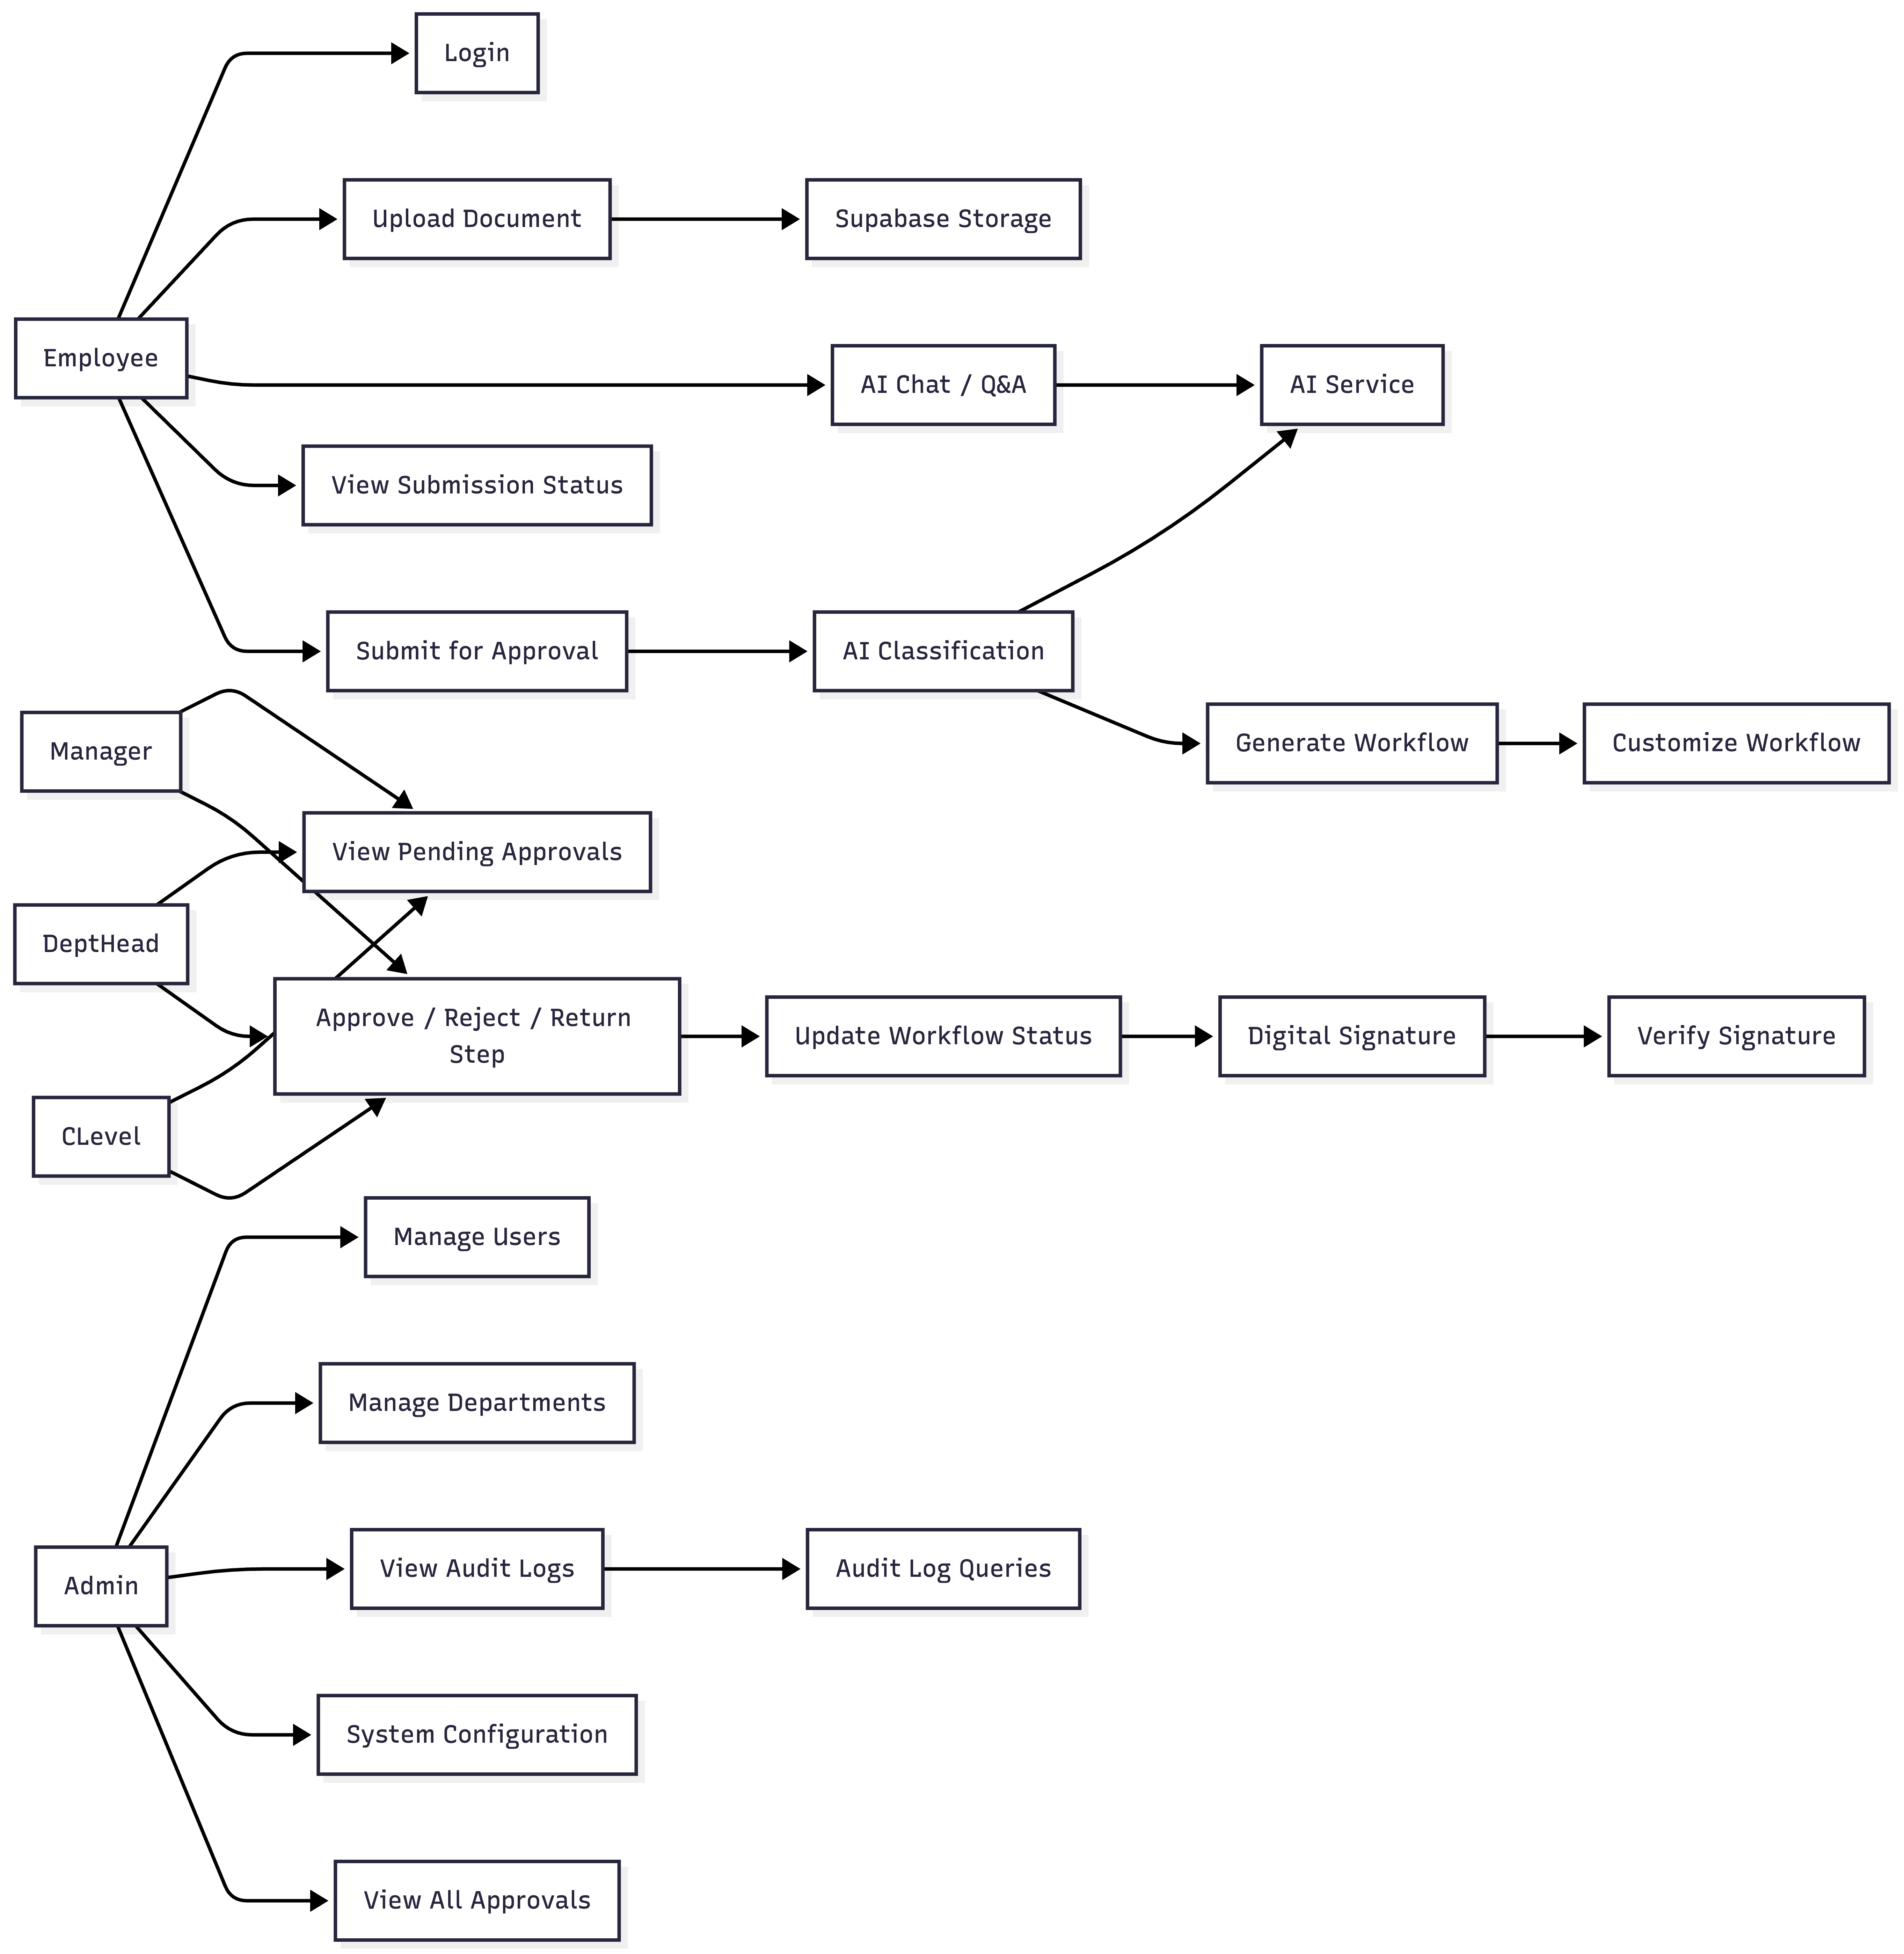
\includegraphics[width=\linewidth]{image/SoftwareDiagram/UseCaseDiagram.png}
  \caption{AgentiX use case diagram.}
  \label{fig:use-case-diagram}
\end{figure}

The use case diagram maps primary actors (Employee, Manager, Dept Head, C\-Level, Admin) to their capabilities: login, upload, AI Q\&A and classification, submit for approval, view pending approvals, monitoring approval status, sign and verify documents, and administrative tasks. It highlights how role-based responsibilities align to system features.

This diagram is useful for validating requirement coverage and ensuring that user stories and access policies correspond to the platform's functional scope, making it a practical bridge between product requirements and system design.

\newpage

\section{Architectural Overview}

The AgentiX platform is structured as a distributed system comprising seven primary layers, each responsible for distinct functional domains. The architecture emphasizes defense-in-depth security, horizontal scalability, and operational observability. All inter-service communication is encrypted using mutual TLS (mTLS), while client-facing interfaces enforce TLS 1.3 for maximum transport security.

The system supports dual deployment models: a managed cloud service with multi-tenant isolation and an enterprise-private offering that integrates directly with organizational infrastructure. Both models share the same core architecture, differing primarily in identity federation strategies and data residency configurations.

\vspace{1em}

\section{Layer-by-Layer Architecture}

\subsection{Client Layer}

The client layer provides three distinct user interfaces, each optimized for specific roles within the approval workflow:

\begin{itemize}
\item \textbf{Web Application (React Next.js):} The primary interface for document submission, approval queue management, and workflow monitoring. Built with React Next.js for server-side rendering and optimal performance, this application serves as the main entry point for document submitters and approvers. It implements responsive design patterns to ensure usability across desktop and tablet form factors.

\item \textbf{Mobile Application:} A dedicated signer interface optimized for mobile devices, enabling executives and department heads to review and approve documents on-the-go. The mobile app implements biometric authentication and supports push notifications for time-sensitive approval requests.

\item \textbf{Admin Console:} A specialized interface for Certificate Authority operations, policy configuration, and audit trail exploration. This console provides tools for managing user roles, configuring approval workflows, monitoring system health, and generating compliance reports.
\end{itemize}

All client applications communicate exclusively with the Edge and Security layer via HTTPS with TLS 1.3, ensuring end-to-end encryption of sensitive document data and user credentials.

\newpage

\subsection{Edge and Security Layer}

This layer serves as the security perimeter for the entire platform, implementing multiple defense mechanisms before requests reach application services:

\begin{itemize}
\item \textbf{API Gateway (NGINX or Envoy):} Acts as the single entry point for all client requests, providing centralized routing, load balancing, and rate limiting. The gateway incorporates a Web Application Firewall (WAF) that filters malicious requests, prevents SQL injection and cross-site scripting attacks, and enforces request size limits to prevent denial-of-service attempts.

\item \textbf{Identity Provider (OIDC/SAML):} Handles authentication and single sign-on integration. For cloud deployments, the platform supports standard OIDC (OpenID Connect) flows, while enterprise-private installations can integrate with existing SAML-based identity providers such as Active Directory Federation Services or Okta. This abstraction ensures seamless integration with organizational identity management systems while maintaining strong authentication standards.
\end{itemize}

After successful authentication, the API Gateway establishes mTLS connections with backend services, ensuring that internal communications are authenticated and encrypted even within the trusted network boundary.

\newpage

\begin{landscape}
\thispagestyle{empty}
\begin{figure}[p]
\centering
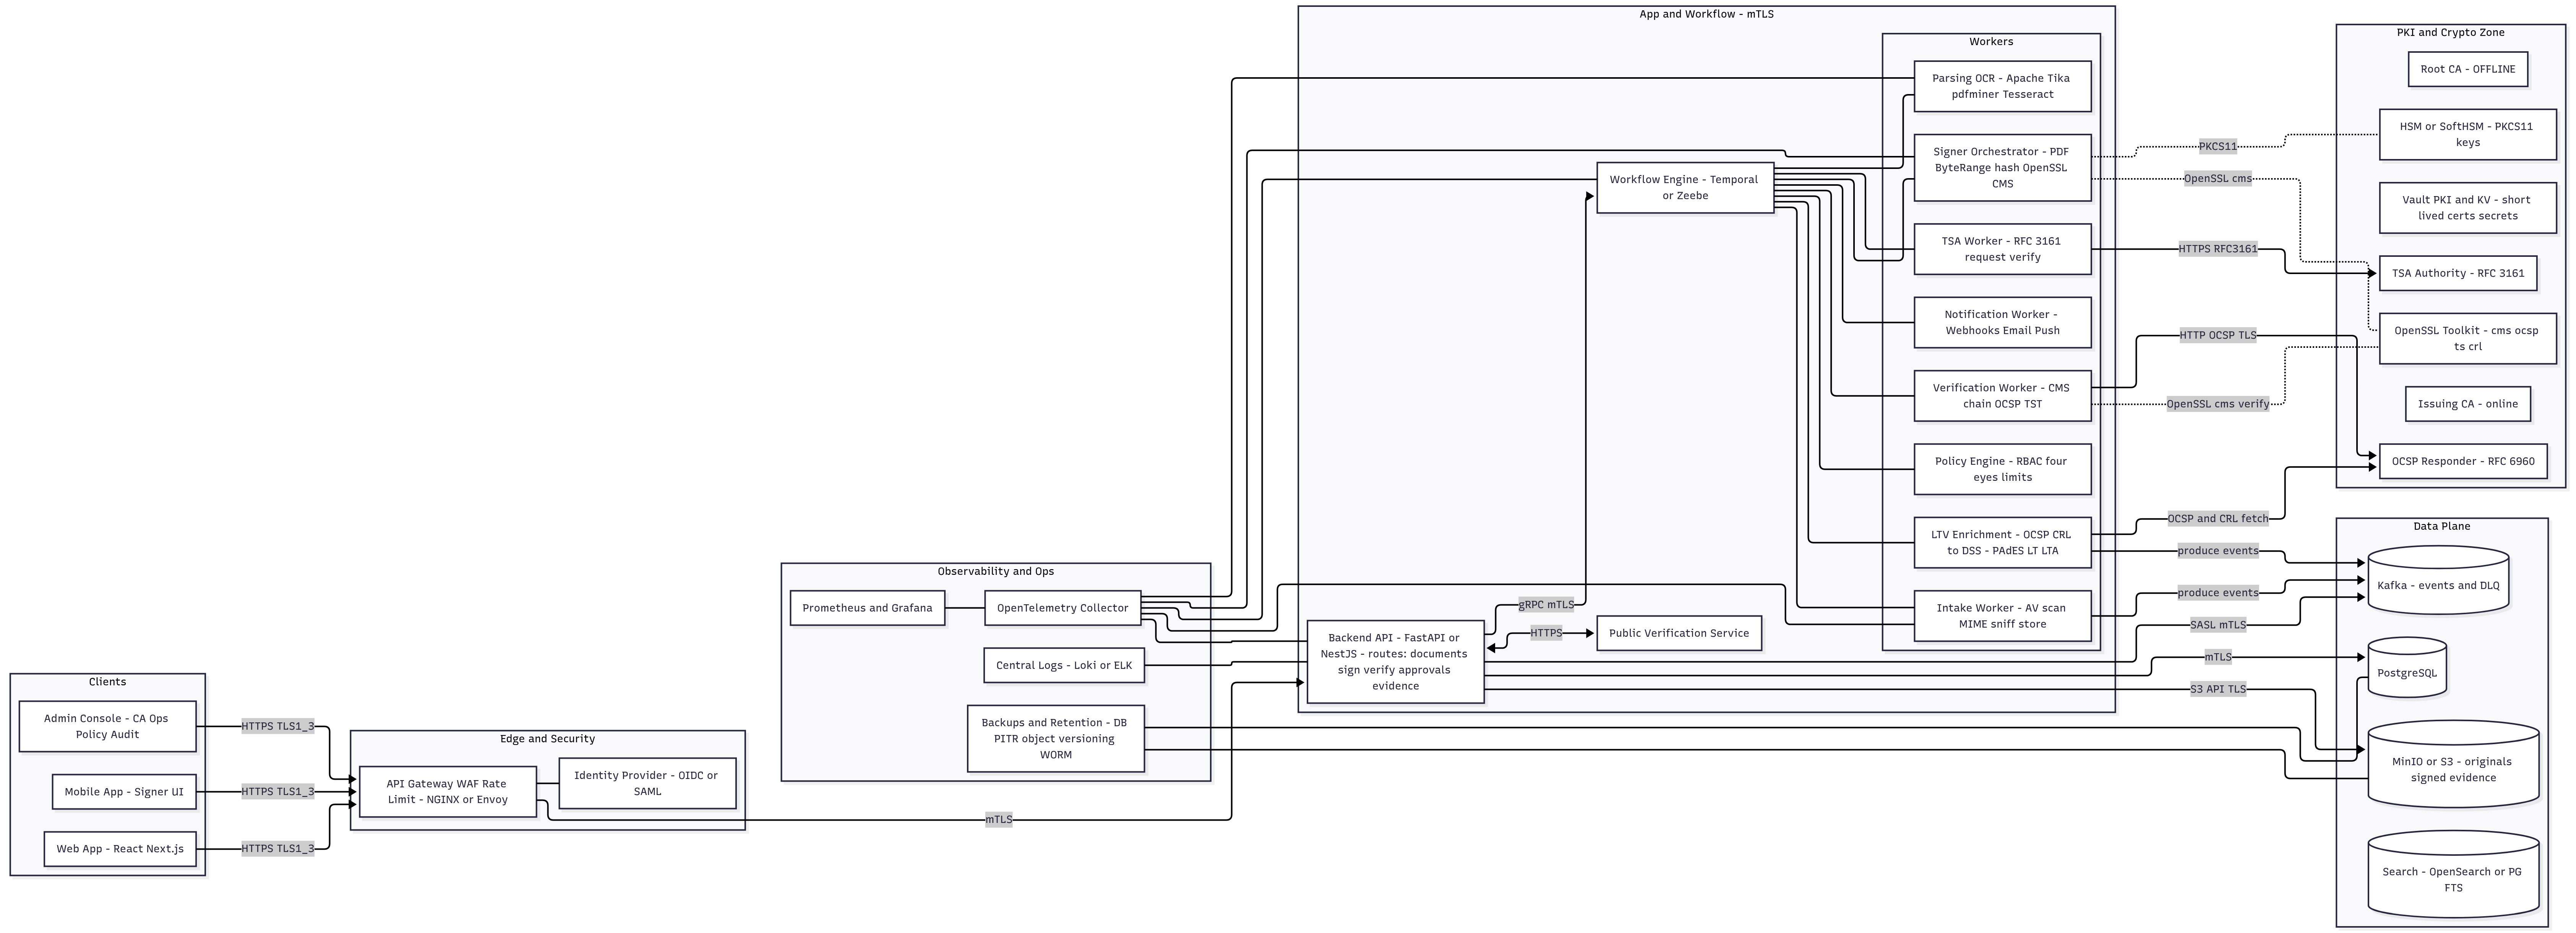
\includegraphics[width=\linewidth,height=\textheight,keepaspectratio]{image/System_Architecture.png}
\caption{AgentiX Complete System Architecture Diagram}
\label{fig:system-architecture}
\end{figure}
\end{landscape}

\newpage

\vspace{1em}

\subsection{Application and Workflow Layer}

The application layer orchestrates core business logic and workflow execution through three primary components:

\begin{itemize}
\item \textbf{Backend API (FastAPI or NestJS):} Implements RESTful and GraphQL endpoints for document operations, signature requests, verification queries, approval actions, and evidence retrieval. The API layer enforces authorization policies, validates input data, and coordinates interactions between the workflow engine and worker services. Built with FastAPI (Python) or NestJS (TypeScript) for high performance and strong typing guarantees.

\item \textbf{Workflow Engine (Temporal or Zeebe):} Manages stateful, long-running approval workflows with guaranteed execution semantics. The workflow engine coordinates the multi-step approval process, handling sequential and parallel approval paths, timeout management, and compensating transactions for rollback scenarios. Temporal or Zeebe provide durable execution guarantees, ensuring that workflows survive service restarts and network partitions without data loss.

\item \textbf{Public Verification Service:} Exposes a standalone endpoint for external parties to verify document signatures without requiring authentication. This service validates cryptographic signatures, checks certificate validity through OCSP (Online Certificate Status Protocol), and returns verification results with detailed attestation metadata.
\end{itemize}

\vspace{1em}

\subsection{Workers Layer}

The workers layer implements specialized microservices, each responsible for a discrete processing task within the document lifecycle. This architecture enables independent scaling, fault isolation, and technology-specific optimizations:

\begin{itemize}
\item \textbf{Intake Worker:} Receives uploaded documents and performs security validation: antivirus scanning, MIME type verification, and file format normalization. Documents passing validation are stored in object storage (MinIO/S3) with metadata persisted to PostgreSQL.

\item \textbf{Parsing and OCR Worker:} Extracts textual content from documents using Apache Tika for general document parsing, pdfminer for PDF text extraction, and Tesseract OCR for scanned images. The extracted text feeds the Agentic AI pipeline for content analysis.

\item \textbf{Policy Engine:} Enforces organizational policies including Role-Based Access Control (RBAC), four-eyes principle (requiring multiple independent approvals), and financial authorization limits. The policy engine validates that proposed approval paths comply with organizational governance rules before workflow initiation.

\item \textbf{Signer Orchestrator:} Coordinates the cryptographic signing process. This worker computes document hashes, interacts with the HSM (Hardware Security Module) via PKCS\#11 interface to perform signing operations, and constructs CMS (Cryptographic Message Syntax) signatures compliant with PDF ByteRange specifications. This ensures that signatures cover the entire document content and are legally defensible.

\item \textbf{TSA Worker:} Requests trusted timestamps from the Time Stamp Authority (TSA) following RFC 3161 standards. Timestamps bind the signature to a specific moment in time, providing evidence that the document was signed before any certificate expiration or revocation.

\item \textbf{LTV Enrichment Worker:} Enhances signatures with Long-Term Validation (LTV) data by embedding OCSP responses and Certificate Revocation Lists (CRLs) into the document. This creates PAdES-LT (PDF Advanced Electronic Signatures - Long Term) or PAdES-LTA (Long Term Archival) compliant documents that remain verifiable even after the original certificates and validation infrastructure are no longer available.

\item \textbf{Verification Worker:} Validates signed documents by verifying CMS signature structures, reconstructing and validating certificate chains, checking OCSP responses, and validating timestamp tokens. This worker implements the bit-matching logic that recomputes document hashes and compares them against signed hash values to detect any tampering.

\item \textbf{Notification Worker:} Delivers approval notifications through multiple channels: webhooks for system integration, email for human recipients, and push notifications for mobile applications. The worker implements retry logic with exponential backoff and dead letter queuing for undeliverable messages.
\end{itemize}

\vspace{1em}

\subsection{PKI and Cryptography Zone}

The PKI layer provides the cryptographic foundation for all signature operations, implementing industry-standard certificate authority functionality with defense-in-depth security:

\begin{itemize}
\item \textbf{Root CA (Offline):} The trust anchor of the PKI hierarchy, stored offline in secure cold storage. The Root CA's private key is used only to sign Issuing CA certificates and is never exposed to network-connected systems, providing maximum protection against compromise.

\item \textbf{Issuing CA (Online):} Issues end-entity certificates for document signers. The Issuing CA operates online but in a hardened environment, signing certificate requests after identity verification and policy validation.

\item \textbf{OCSP Responder (RFC 6960):} Provides real-time certificate status information, responding to OCSP queries with signed responses indicating whether certificates are valid, revoked, or unknown. This service is critical for LTV validation workflows.

\item \textbf{TSA Authority (RFC 3161):} Issues cryptographically signed timestamps that bind documents to specific points in time. The TSA maintains a secure time source and signs timestamp tokens with its own certificate, providing non-repudiable proof of document existence at the timestamp moment.

\item \textbf{HSM or SoftHSM (PKCS\#11):} Stores cryptographic private keys in tamper-resistant hardware (HSM) or software emulation (SoftHSM for development). Keys never leave the HSM boundary; all signing operations occur within the module through PKCS\#11 interface calls.

\item \textbf{OpenSSL Toolkit:} Provides low-level cryptographic operations including CMS signature generation/verification, OCSP request/response handling, timestamp request/verification, and CRL management. OpenSSL serves as the cryptographic engine underlying higher-level PKI services.

\item \textbf{Vault PKI and KV:} HashiCorp Vault manages short-lived certificates for service-to-service mTLS authentication and stores sensitive configuration secrets. Vault's PKI engine automates certificate issuance and rotation, while the Key-Value store securely manages API keys, database credentials, and encryption keys.
\end{itemize}

\vspace{1em}

\subsection{Data Plane}

The data plane provides persistent storage for all platform data, optimized for different access patterns and durability requirements:

\begin{itemize}
\item \textbf{PostgreSQL:} The primary relational database stores user accounts, document metadata, workflow states, approval records, and audit logs. PostgreSQL's ACID guarantees ensure data consistency across concurrent transactions, while advanced features like row-level security and table partitioning support multi-tenant isolation and performance optimization.

\item \textbf{MinIO or Amazon S3:} Object storage holds original documents, signed versions, signature evidence packages, and archived materials. Object storage provides virtually unlimited scalability, versioning capabilities to track document revisions, and lifecycle policies for automated archival and deletion according to retention requirements.

\item \textbf{Apache Kafka:} Event streaming platform enables asynchronous communication between services. Workers publish events (document uploaded, signature completed, approval granted) to Kafka topics, allowing consumers to react without tight coupling. Kafka's Dead Letter Queue (DLQ) captures failed message processing for later investigation and reprocessing.

\item \textbf{OpenSearch or PostgreSQL Full-Text Search:} Enables rapid document discovery through full-text search across document content, metadata, and annotations. Search indices are continuously updated as documents progress through the approval workflow, ensuring users can find relevant documents regardless of their current state.
\end{itemize}

\vspace{1em}

\subsection{Observability and Operations Layer}

The observability layer provides comprehensive visibility into system behavior, supporting proactive monitoring, incident response, and capacity planning:

\begin{itemize}
\item \textbf{OpenTelemetry Collector:} Ingests distributed traces, metrics, and logs from all application services and workers. OpenTelemetry's vendor-neutral instrumentation enables consistent observability across polyglot microservices, correlating requests as they flow through multiple components.

\item \textbf{Prometheus and Grafana:} Prometheus scrapes time-series metrics from instrumented services, storing them in a highly efficient time-series database. Grafana visualizes these metrics through customizable dashboards, tracking key performance indicators like approval latency, signature success rates, and worker queue depths. Alert rules trigger notifications when metrics exceed defined thresholds.

\item \textbf{Centralized Logs (Loki or ELK):} Aggregates log streams from all services into a searchable central repository. Loki (with Grafana) or the ELK stack (Elasticsearch, Logstash, Kibana) enable operators to search logs across services, correlate events during incident investigations, and establish audit trails for compliance reporting.

\item \textbf{Backups and Retention:} Implements comprehensive data protection strategies including PostgreSQL point-in-time recovery (PITR), object storage versioning with immutable retention periods, and Write-Once-Read-Many (WORM) storage for tamper-proof archival. Automated backup testing ensures recovery procedures remain effective.
\end{itemize}

\vspace{1em}

\section{Security Architecture}

Security permeates every layer of the AgentiX architecture through multiple complementary mechanisms:

\begin{itemize}
\item \textbf{Transport Security:} TLS 1.3 encrypts all client-to-gateway communication with forward secrecy, while mTLS secures all service-to-service communication within the trusted network boundary. Certificate rotation is automated through Vault's PKI engine.

\item \textbf{Authentication and Authorization:} The Identity Provider centralizes authentication with support for multi-factor authentication (MFA), while the Backend API enforces fine-grained authorization using attribute-based access control (ABAC) policies that consider user roles, document sensitivity, and approval context.

\item \textbf{Cryptographic Integrity:} The Signer Orchestrator computes SHA-256 or SHA-3 hashes of document content before signing, while the Verification Worker recomputes hashes to detect tampering. HSM-backed signing ensures private keys never exist in plaintext outside secure hardware boundaries.

\item \textbf{Audit and Compliance:} Every document access, approval action, and signature operation generates immutable audit log entries in PostgreSQL with cryptographic chaining to prevent retroactive modification. These logs support regulatory compliance reporting and forensic investigations.

\item \textbf{Defense in Depth:} Multiple security layers ensure that compromise of any single component does not expose the entire system. The API Gateway filters malicious requests, the Policy Engine validates business rules, and the PKI zone isolates cryptographic operations in hardened enclaves.
\end{itemize}

\vspace{1em}

\section{Scalability and Resilience}

The microservices architecture enables independent scaling of components based on load characteristics:

\begin{itemize}
\item \textbf{Horizontal Scaling:} Stateless workers and API services can be replicated horizontally behind load balancers, distributing request processing across multiple instances. Kafka enables workers to process messages in parallel, automatically load-balancing across consumer instances.

\item \textbf{Workflow Durability:} Temporal/Zeebe workflow engines persist workflow state to PostgreSQL, ensuring that long-running approval processes survive service restarts, deployments, and infrastructure failures without data loss or duplicate processing.

\item \textbf{Fault Isolation:} Circuit breakers prevent cascading failures when downstream services become unavailable. Workers implement exponential backoff retry logic, while Kafka's DLQ captures messages that fail processing after configured retry attempts.

\item \textbf{Data Durability:} PostgreSQL streaming replication maintains standby replicas for high availability, while object storage replicates documents across multiple availability zones. Regular backup testing validates that disaster recovery procedures meet defined Recovery Point Objective (RPO) and Recovery Time Objective (RTO) targets.
\end{itemize}

\vspace{1em}

\section{Deployment Models}

AgentiX supports two deployment configurations to accommodate diverse organizational requirements:

\begin{itemize}
\item \textbf{Managed Cloud Service:} A multi-tenant SaaS offering hosted on public cloud infrastructure (AWS, Azure, or GCP). Tenant isolation is enforced at the database schema level and through resource namespacing in Kubernetes. Each tenant receives a dedicated admin console for self-service configuration of approval workflows, user roles, and integration settings. The cloud service provides automated provisioning, managed upgrades, and 24/7 operational support.

\item \textbf{Enterprise-Private Deployment:} A single-tenant installation within the customer's private network, deployed using containerized services (Docker/Kubernetes) and infrastructure-as-code templates (Terraform/Helm). This model enables direct integration with on-premise databases, HR systems, and identity providers through VPN or private network connectivity. Customers maintain full control over data residency, network policies, and compliance configurations.
\end{itemize}

Both deployment models share the same core architecture, with configuration differences limited to identity federation (OIDC vs. SAML), network topology (public vs. private), and operational responsibilities (managed vs. self-hosted).

\vspace{1em}

\section{Integration Architecture}

AgentiX provides multiple integration mechanisms to embed within existing enterprise ecosystems:

\begin{itemize}
\item \textbf{RESTful and GraphQL APIs:} The Backend API exposes comprehensive programmatic interfaces for document submission, approval automation, signature verification, and audit trail retrieval. API clients authenticate using OAuth 2.0 bearer tokens or API keys with configurable scopes.

\item \textbf{Webhook Notifications:} The Notification Worker delivers real-time event notifications to external systems via configurable webhooks, enabling workflow integration with CRM systems, document management platforms, and business intelligence tools.

\item \textbf{Identity Federation:} Support for OIDC, SAML, and LDAP protocols enables seamless integration with enterprise identity providers including Azure AD, Okta, Auth0, and on-premise Active Directory installations.

\item \textbf{SCIM Provisioning:} The System for Cross-domain Identity Management (SCIM) protocol automates user and group synchronization between enterprise HR systems and AgentiX, ensuring that organizational changes automatically propagate to approval workflows.
\end{itemize}

\vspace{1em}

\section{Technology Stack Summary}

The following table summarizes key technology choices across architectural layers:

\begin{table}[h!]
\centering
\footnotesize
\renewcommand{\arraystretch}{1.3}
\begin{tabular}{|p{0.28\textwidth}|p{0.60\textwidth}|}
\hline
\textbf{Component} & \textbf{Technology Options} \\ \hline
Frontend Applications & React Next.js, React Native, TypeScript \\ \hline
API Gateway & NGINX, Envoy Proxy \\ \hline
Backend API & FastAPI (Python), NestJS (TypeScript) \\ \hline
Workflow Engine & Temporal, Zeebe \\ \hline
Message Broker & Apache Kafka \\ \hline
Relational Database & PostgreSQL with TimescaleDB extension \\ \hline
Object Storage & MinIO (self-hosted), Amazon S3 \\ \hline
Search Engine & OpenSearch, PostgreSQL Full-Text Search \\ \hline
PKI and Cryptography & OpenSSL, SoftHSM, Hardware HSM (Thales, Utimaco) \\ \hline
Secrets Management & HashiCorp Vault \\ \hline
Observability & OpenTelemetry, Prometheus, Grafana, Loki, ELK \\ \hline
Container Orchestration & Kubernetes, Docker Compose \\ \hline
Infrastructure as Code & Terraform, Helm Charts \\ \hline
\end{tabular}
\vspace{0.6em}
\caption{AgentiX technology stack across architectural layers}
\label{tab:tech-stack}
\end{table}

\vspace{1em}

\section{Architectural Principles}

The AgentiX architecture adheres to the following design principles:

\begin{itemize}
\item \textbf{Security by Design:} Security considerations inform every architectural decision, from transport encryption and authentication to data encryption at rest and cryptographic signature validation.

\item \textbf{Separation of Concerns:} Each microservice encapsulates a single responsibility, enabling independent development, testing, deployment, and scaling without impacting other components.

\item \textbf{API-First Design:} All functionality is exposed through well-defined APIs with comprehensive documentation, enabling programmatic integration and supporting multiple client applications.

\item \textbf{Event-Driven Architecture:} Asynchronous event streaming through Kafka decouples services, enabling independent scaling and fault isolation while maintaining eventual consistency.

\item \textbf{Operational Excellence:} Comprehensive observability, automated deployment pipelines, and infrastructure-as-code practices ensure reliable operations at scale.\sloppy

\item \textbf{Standards Compliance:} Adherence to established standards (RFC 3161 for timestamps, RFC 6960 for OCSP, PAdES for PDF signatures) ensures interoperability and legal defensibility.
\end{itemize}

\vspace{1em}

This architecture provides a robust foundation for implementing AgentiX's intelligent document approval capabilities while ensuring security, scalability, and operational reliability required for enterprise deployments.

\section{User Journey}

This section provides a comprehensive, end-to-end narrative of the user
journey in AgentiX. It describes the primary personas, the sequence of
interactions between users and the system, and the internal processing
stages that convert a submitted document into a cryptographically
signed, auditable artifact. The chapter links UX-level actions to the
architectural components described in the Architecture and Design
chapter, and outlines success metrics, exception handling, and
observability touchpoints to support real-world adoption.

\subsection{Personas and Roles}

The following personas represent the typical actors who interact with
AgentiX. Understanding their goals and constraints informs the design
of the user journey and the decisions made by the Agentic AI.

\begin{itemize}
  \item \textbf{Submitter}: Prepares and uploads documents, populates
    metadata, and initiates the approval workflow. Usually a business
    user (project manager, HR, procurement).
  \item \textbf{Reviewer / Approver}: A role-based actor (legal reviewer,
    finance approver, C-level signatory) who receives a request, reviews
    content, provides comments, and approves or rejects.
  \item \textbf{System Administrator}: Manages organizational policies,
    identity federation, and certificate lifecycle; reviews audit logs
    and resolves escalations.
  \item \textbf{Agentic AI}: An orchestration layer that analyzes
    documents, suggests approval flows, and coordinates workers and
    services to execute the workflow.
\end{itemize}

\subsubsection{High-level Flow}

At a high level, the user journey follows these stages (expanded later):

\begin{enumerate}
  \item Submission and validation
  \item Pre-processing (OCR, parsing)
  \item Document understanding and classification
  \item Workflow suggestion and user confirmation
  \item Execution of approval steps and return-loop handling
  \item Cryptographic signing, timestamping, and archival
  \item Verification and public attestation
\end{enumerate}

Each stage maps to specific components in the architecture: the Web
Application for UI interactions, Intake and Parsing workers for
pre-processing, the Agentic AI and Policy Engine for workflow
decisions, the Workflow Engine for orchestration, the Signer
Orchestrator and PKI zone for signing, and the Data Plane for storage
and audit.

\subsection{Detailed Journey}

This section expands each stage with concrete steps, inputs/outputs, and
error handling considerations.

\subsubsection{Submission and Validation}

The Submitter uploads a document through the Submit module or the
conversational UI. Required metadata (title, requester, department,
deadline, sensitivity) is captured, either manually or via AI-assisted
parsing of the uploaded file. On receipt, the Intake Worker performs a
series of validations:

\begin{itemize}
  \item Antivirus scan and MIME type verification.
  \item File size and format checks (rejecting unsupported types).
  \item Metadata validation against organizational policy (required
    fields, SLA tiers).
\end{itemize}

If any validation fails, the submitter receives an immediate, human-
readable error message with remediation steps; events are emitted to
Kafka for observability and retry logic where appropriate.

\subsubsection{Pre-processing: Parsing and OCR}

Once validated, the Parsing and OCR Worker extracts machine-readable
text and structural metadata from the document. For born-digital PDFs
the system uses robust PDF text extraction; for scanned images it
applies Tesseract with language-specific models. The extracted text is
normalized and indexed for fast search.

Outputs from this stage include: the full-text payload, detected
language(s), extracted entities (dates, monetary values, party names),
and a confidence score per extraction.

Failure modes at this stage (e.g., unreadable scan) trigger a
submission status of \emph{Needs Attention} and notify the submitter to
reupload or supply a higher-quality source. Low-confidence extraction
is surfaced on the classification page so approvers can review and
correct any critical metadata before the workflow proceeds.

\subsubsection{Document Understanding and Classification}

The Agentic AI ingests the normalized text and metadata to perform:

\begin{itemize}
  \item Semantic classification (contract, invoice, NDA, HR form, etc.).
  \item Risk assessment (privacy-sensitive data present, financial
    impact level, regulatory flags).
  \item Signatory inference (who must sign, mandatory approvers).
\end{itemize}

The model returns a structured proposal: a ranked list of candidate
approval steps, estimated SLAs per step, and an explanation token that
highlights the evidence used (key sentences and entities). The
explainability artifact is exposed in the UI to aid transparency and
compliance.

\subsubsection{Workflow Suggestion and User Confirmation}

The proposed workflow is presented to the Submitter in an interactive
view. Key features include:

\begin{itemize}
  \item A visual timeline showing sequential and parallel steps.
  \item Editable approver assignments with search-enabled person
    selection backed by SCIM/LDAP.
  \item SLA toggles to adjust urgency and escalation levels.
  \item A confidence indicator and the AI's textual rationale for
    each suggested step.
\end{itemize}

The Submitter may accept the suggested flow, modify it, or request a
manual override. Any manual change is captured as part of the workflow
definition and recorded in the audit trail.

\subsubsection{Approval Execution and Return-loop Handling}

Once the workflow is initiated, the Workflow Engine creates durable
executions for each step. Approvers receive notifications via the
Notification Worker (email, push, or webhook) and act through the
Approval Dashboard or mobile signer interface. Each approval action
produces an immutable record including comments, timestamp, and actor
identity.

The return-loop (intelligent rejection routing) follows this logic:

\begin{itemize}
  \item If an approver rejects, they must select a rejection reason and
    optionally designate a responsible role or individual to receive the
    correction task.
  \item The system routes the document directly to the responsible
    role (not always back to the original submitter) to minimize
    friction and avoid redundant handoffs.
  \item The Policy Engine enforces constraints (e.g., certain rejection
    reasons may trigger mandatory second reviews or legal involvement).
\end{itemize}

Retries, escalations, and SLA breaches are handled by the Workflow
Engine with compensating actions and notifications; unresolved
exceptions escalate to the System Administrator queue.

\subsubsection{Signing, Timestamping, and Archival}

When all approval steps are complete, the Signer Orchestrator performs
the signing sequence:

\begin{enumerate}
  \item Compute canonical hash of the final document payload (SHA-256).
  \item Request HSM to perform private-key signing (PKCS\#11 API).
  \item Request trusted timestamp from the TSA (RFC 3161) and embed
    the timestamp token.
  \item Generate LTV data (OCSP/CRL evidence) and attach to the
    signature package for future verification.
  \item Store the signed artifact and metadata in object storage with
    retention policy tags.
\end{enumerate}

All signature operations generate an auditable trail linking signing
keys, certificate chain, timestamp, and the bit-matching evidence used
for verification.

\subsubsection{Verification and Public Attestation}

AgentiX exposes a Public Verification Service that allows external
parties to validate a document's signature without requiring internal
credentials. The verification returns an attestation record including
timestamp, certificate chain validity, and a tamper-status boolean
(based on recomputed hash vs signed hash). For internal investigations
or audits, the Verification Worker can perform deep checks including
certificate revocation status and archived OCSP responses.

\subsection{State Machine and Possible States}

The document lifecycle is modeled as a finite-state machine. Primary
states include: \texttt{Draft}, \texttt{Pending}, \texttt{In-Review},
\texttt{Approved}, \texttt{Rejected}, \texttt{Signed}, and
\texttt{Archived}. Transitions are triggered by user actions
(submit/approve/reject) or system events (timeout/escalation/sign).

Key invariants enforced by the Policy Engine:

\begin{itemize}
  \item A document cannot transition to \texttt{Signed} unless all
    required approvals are present and cryptographic checks pass.
  \item Rejections must record a responsible role for the correction
    route to preserve the intelligent return-loop behavior.
  \item SLA breaches emit alerts and may auto-escalate to a backup
    approver based on configured policies.
\end{itemize}

\subsection{Metrics, Observability, and Success Criteria}

Primary metrics to track the health and effectiveness of the user
journey include:

\begin{itemize}
  \item Time-to-first-approval (submit -> first approver action).
  \item End-to-end approval time (submit -> signed).
  \item Return-loop rate (percentage of workflows that required
    rework).
  \item AI suggestion acceptance rate (percentage of suggested flows
    accepted without modification).
  \item Signature success rate and verification false-positive/false-
    negative rates.
\end{itemize}

These metrics are emitted as Prometheus counters and histograms, with
dashboards in Grafana and alerting rules for SLA violations.

\subsection{UX, Accessibility, and Internationalisation}

The journey is designed to be accessible and localizable: the UI
supports Thai and English locales, keyboard navigation, and ARIA
attributes for screen readers. The conversational UI includes a
lightweight fallback form for environments where the chat-style
interaction is unavailable or when assistive technologies require a
simpler input model.

\subsection{Privacy, Security, and Compliance Considerations}

Privacy is enforced by minimizing PII in AI prompts, redacting sensitive
snippets in logs, and encrypting documents at rest with per-tenant
keys. The Policy Engine applies data classification rules to avoid
sending regulated content to external AI endpoints unless explicitly
allowed by policy.

\section{Web Application Features and Design}

This section details the comprehensive design and feature set of the developed web platform, \textbf{AgentiX}. AgentiX is an enterprise-grade document approval and orchestration platform powered by Agentic AI. The application is designed to solve complex organizational challenges related to document routing, compliance monitoring, and secure cryptographic signing.

\subsection{Technical Architecture}
The user interface (UI) is built using a modern \textbf{React} ecosystem to ensure a responsive and interactive experience.

\begin{itemize}
\item \textbf{Core Framework:} React with Vite for high-performance local development and optimized production builds.
\item \textbf{Styling:} \textbf{Tailwind CSS} is employed for a utility-first styling approach, allowing for rapid UI development and consistent design language (e.g., standardized color palettes, spacing, and typography).
\item \textbf{Component Library:} A modular architecture using \textbf{Shadcn UI} (built on top of Radix UI primitives) ensures accessibility compliance with Web Accessibility Initiative – Accessible Rich Internet Applications (WAI-ARIA) and provides robust, pre-built components like Dialogs, Cards, and Popovers.
\item \textbf{Iconography:} \textbf{Lucide React} is used for consistent, lightweight, and scalable vector icons throughout the application.
\end{itemize}

The platform is structured around six core modules, navigable via a persistent sidebar interface: \textbf{Home}, \textbf{Submit} (Workflow Engine), \textbf{Dashboard}, \textbf{Admin}, \textbf{Signature}, and \textbf{Tutorial}. This layout ensures that users always have context of their location within the application while keeping key navigation tools readily accessible.

\vspace{1em}

\subsection{Landing Page (Home)}

\begin{figure}[htbp]
    \centering
    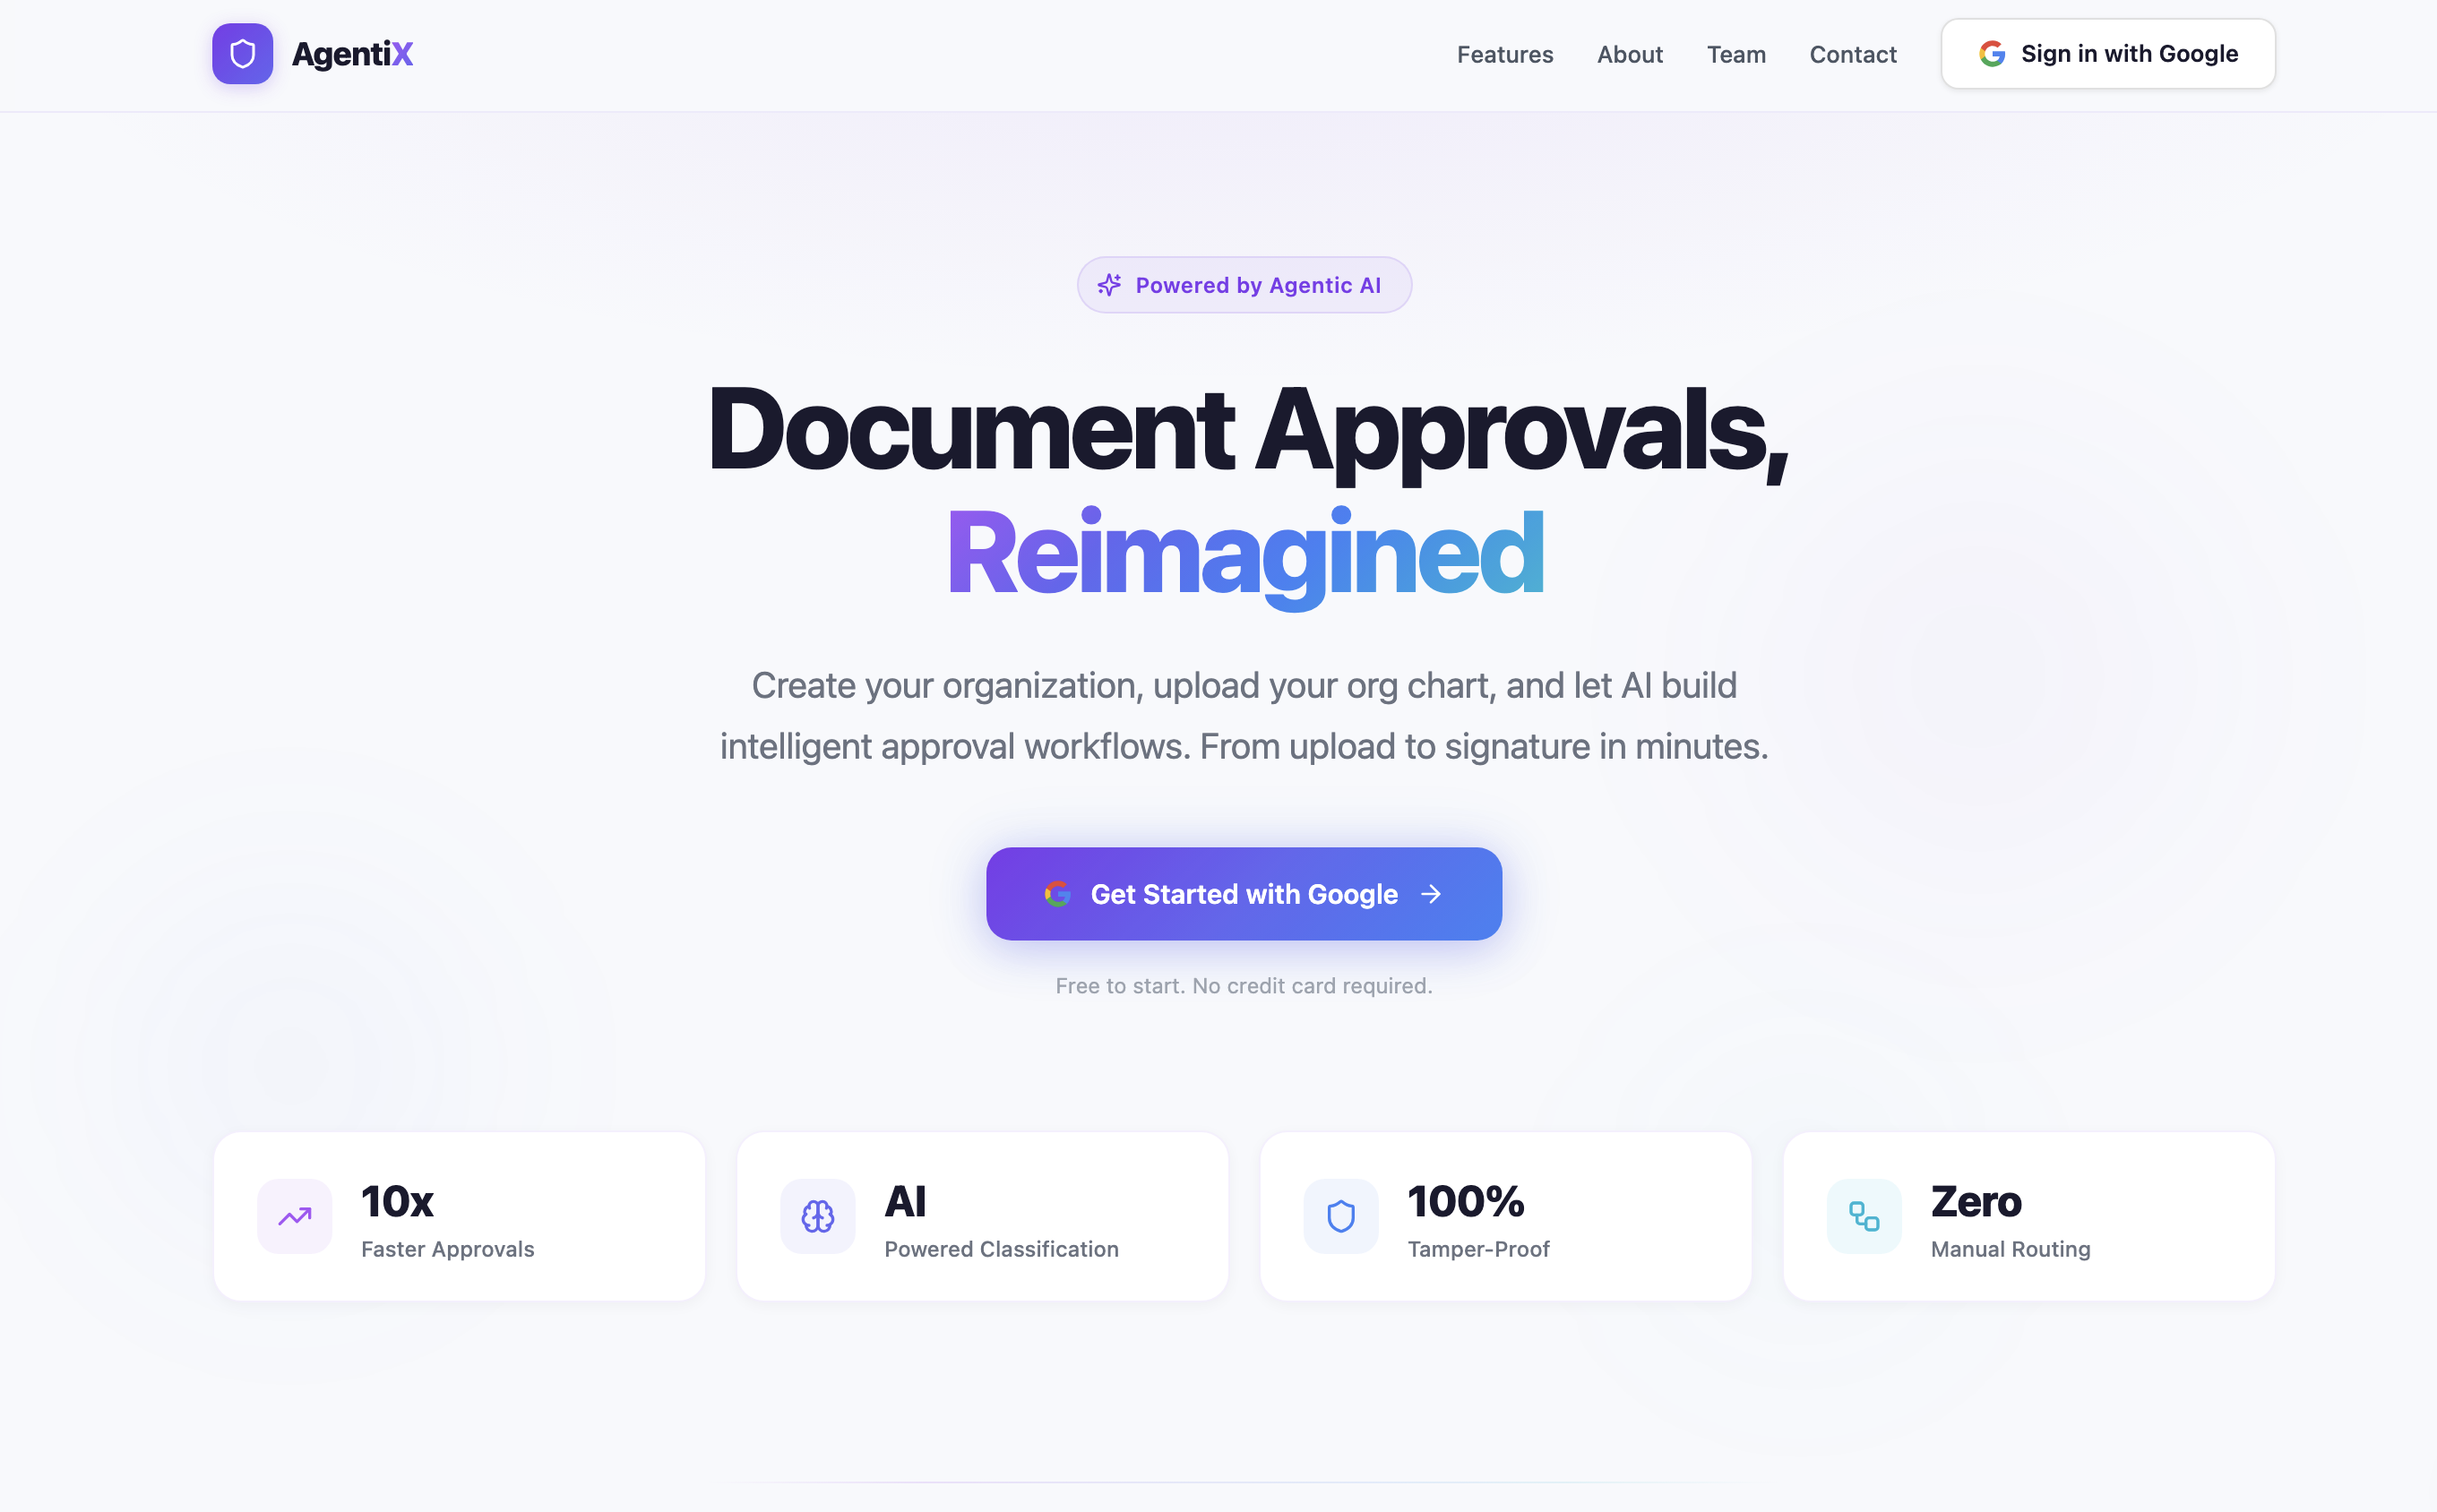
\includegraphics[width=0.9\linewidth]{image/landing_page_placeholder.png}
    \caption{AgentiX Landing Page Interface}
    \label{fig:landing_page}
\end{figure}
The Landing Page is the public-facing entrance to AgentiX and the primary trust-building surface for prospective enterprise customers. The design emphasises clarity, credibility, and an immediate path to action: quick onboarding, clear security assurances, and succinct benefit statements.

\subsubsection{Hero Section}
The Hero occupies the top of the page and uses a soft gradient background, large typographic scale, and a concise value proposition to capture attention. The headline shown on the screenshots — ``Document Approvals, Reimagined'' — is supported by a short explanatory subheading and a single, prominent call-to-action.

\begin{itemize}
\item \textbf{Headline:} ``Document Approvals, Reimagined.'' The heading communicates the product's transformative promise with a confident, modern tone.
\item \textbf{Supporting copy:} A single sentence describes the workflow: ``Create your organization, upload your org chart, and let AI build intelligent approval workflows. From upload to signature in minutes.'' This explains the user benefit in plain language.
\item \textbf{Primary CTA:} A visually prominent button (e.g., \texttt{Get Started with Google}) is styled to draw the eye and communicates a low-friction sign-up path: ``Free to start. No credit card required.'' 
\item \textbf{Trust Badge:} A small, non-distracting badge reads ``Powered by Agentic AI'' and sits above or near the headline to reinforce technological credibility.
\end{itemize}

\subsubsection{Top-Level Benefits and Metrics}
Beneath the hero, a horizontal row of compact benefit cards succinctly communicates measurable outcomes and differentiators. The screenshots emphasise four short claims that can be scanned quickly:

\begin{itemize}
\item \textbf{10x:} Faster Approvals — indicates relative speed improvements.
\item \textbf{AI:} Powered Classification — highlights the AI-driven routing and classification capability.
\item \textbf{100\%:} Tamper-Proof — communicates integrity and cryptographic signing guarantees.
\item \textbf{Zero:} Manual Routing — emphasizes elimination of manual steps via automation.
\end{itemize}

\subsubsection{Feature Cards}
A set of four feature cards presents core capabilities with a single-line title and 1--2 sentence description mirroring the visual layout in the images. The cards are designed for quick comprehension and to act as entry points into deeper documentation or product pages.

\begin{itemize}
\item \textbf{AI Classification:} Upload any document — the system reads, classifies, assesses risk, and routes to the right approvers automatically.
\item \textbf{Smart Routing:} Approval workflows are generated from your organisation structure so the right people, in the right order, are notified every time.
\item \textbf{Digital Signatures:} RSA-2048 cryptographic signatures are embedded at the bit level; any tampering is instantly detected and verifiable.
\item \textbf{Intelligent Return Loop:} Rejected documents are routed back to the responsible party (not the original submitter) to accelerate correction and resubmission.
\end{itemize}

\vspace{1em}

\subsection{Homepage After Login}
\begin{figure}[htbp]
  \centering
  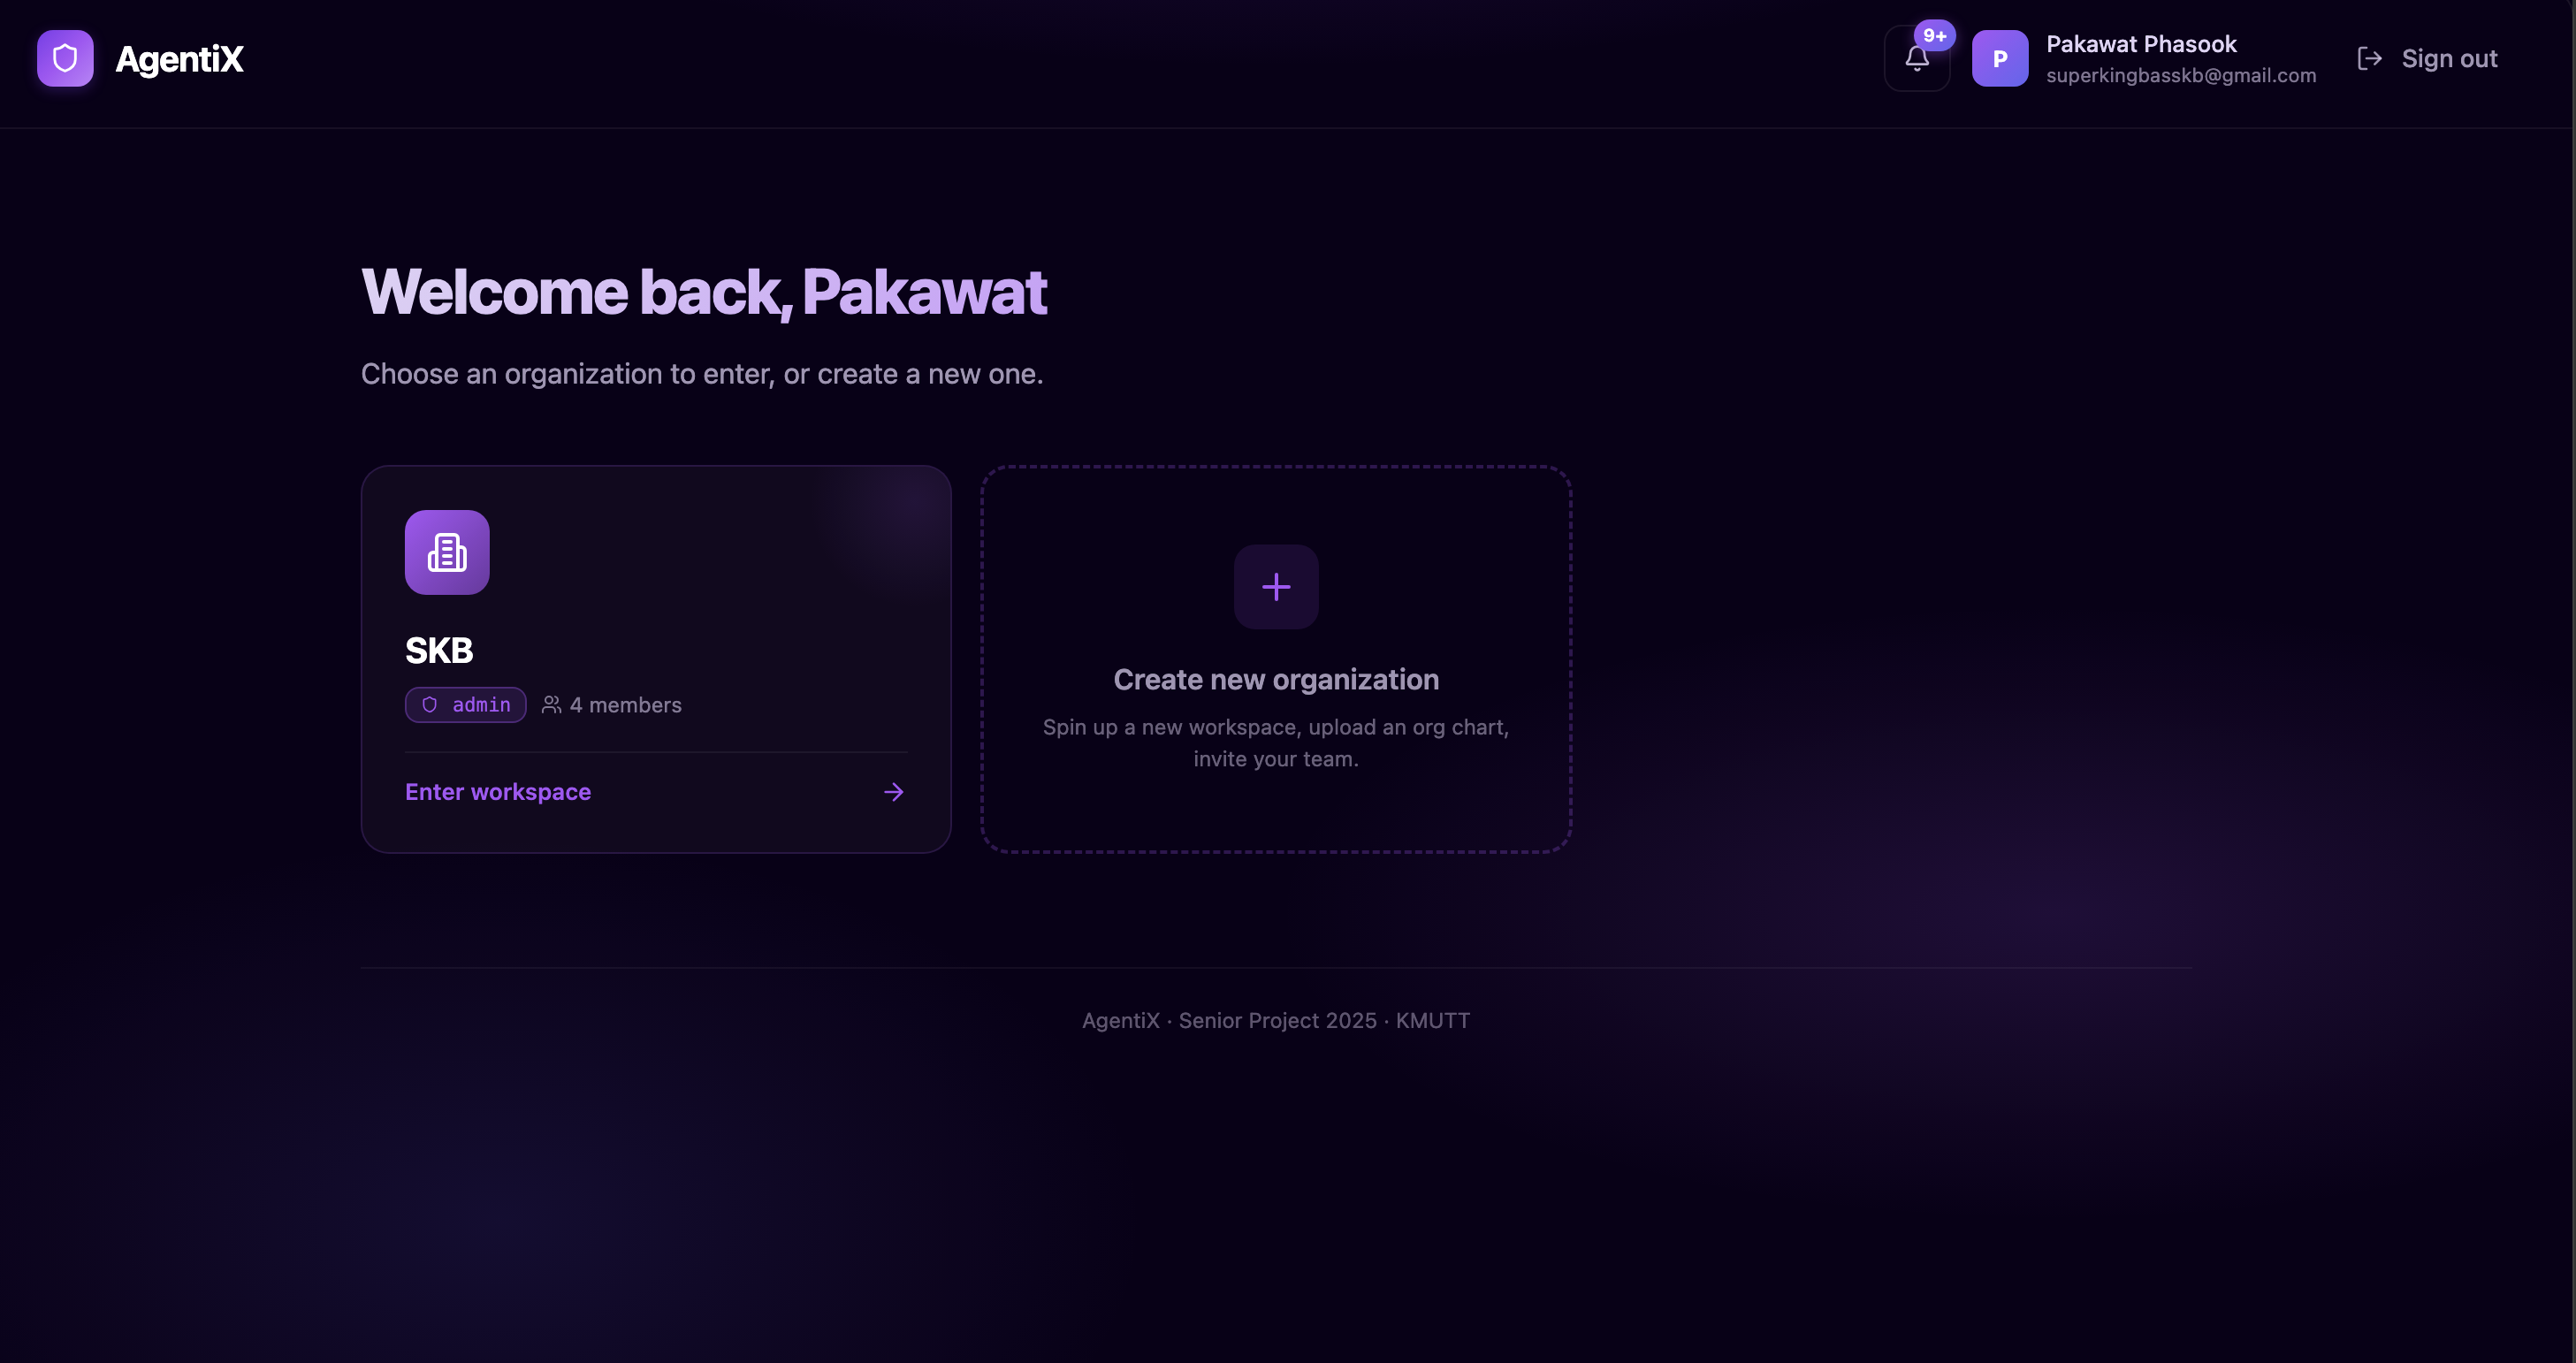
\includegraphics[width=0.48\linewidth]{image/workspace_placeholder.png}
  \hfill
  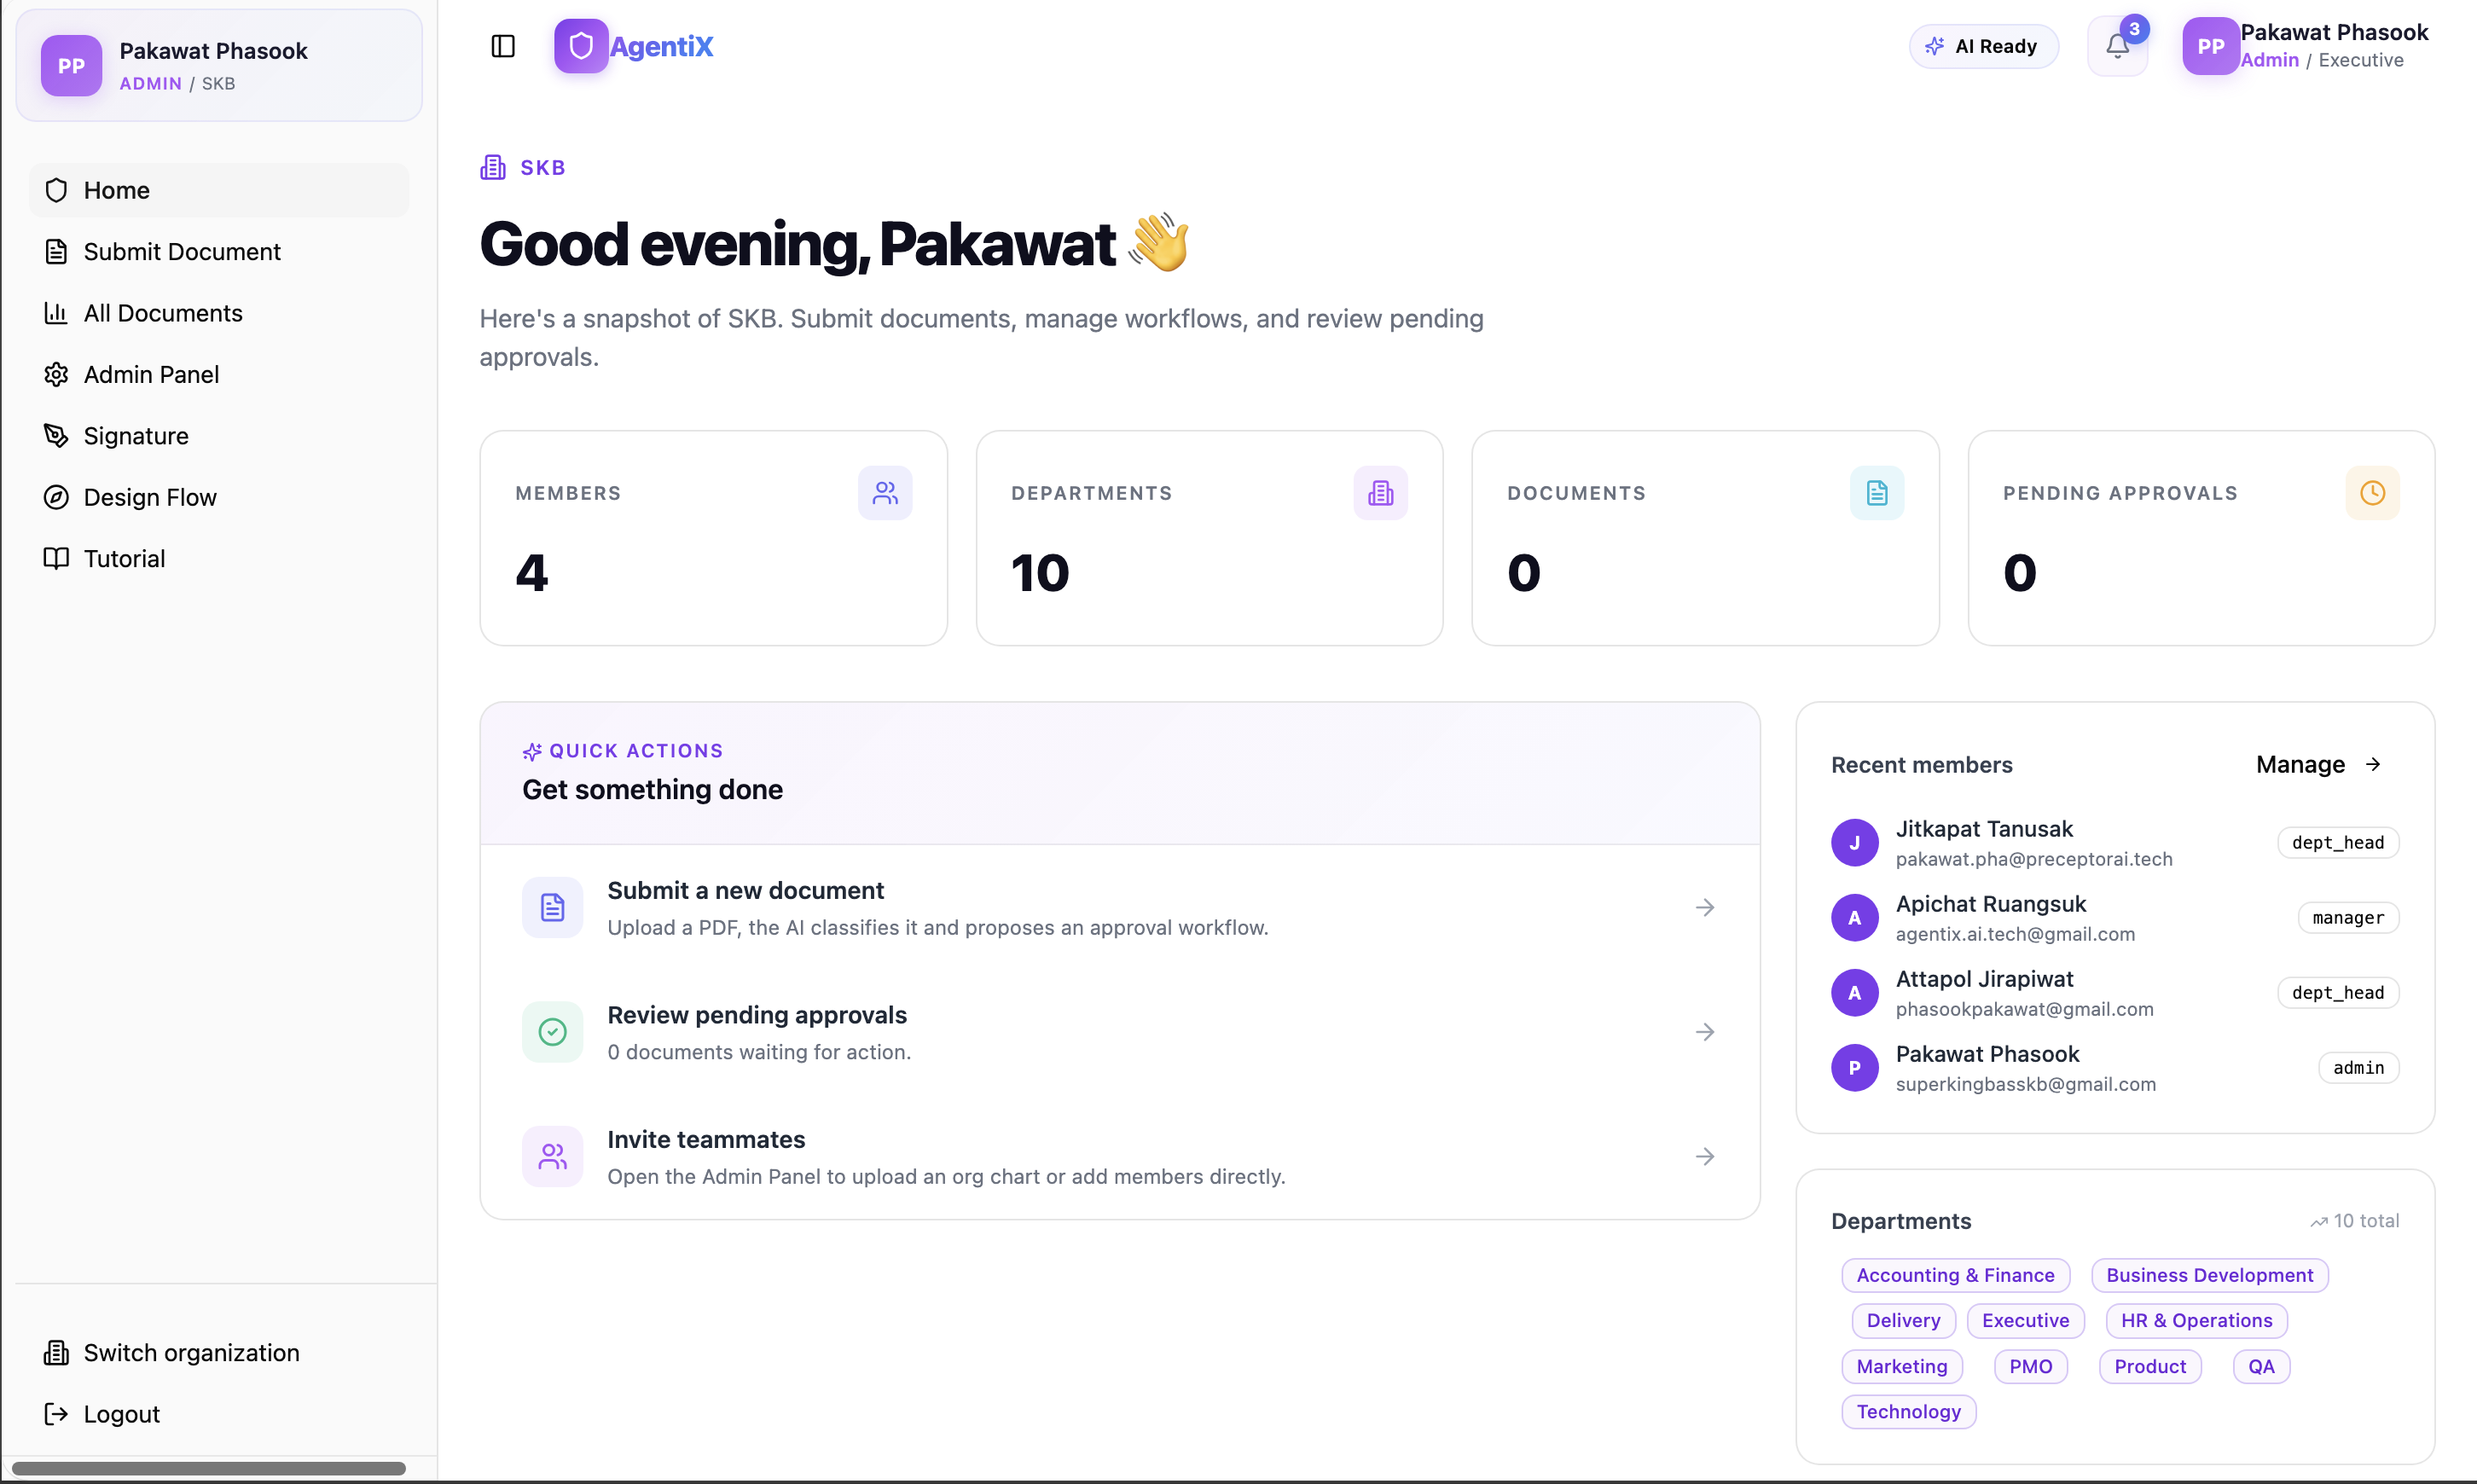
\includegraphics[width=0.48\linewidth]{image/main_dashboard_placeholder.png}
  \caption{Homepage after login: left — organisation selector with "Create new organization" card; right — example workspace card and workspace entry.}
  \label{fig:homepage_after_login}
\end{figure}

After authentication, users land on an organisation-centric homepage that prioritises fast access to workspaces and immediate context about membership and roles. The attached screenshots (Figure~\ref{fig:homepage_after_login}) illustrate the principal UI elements and interaction patterns used on this screen:

\begin{itemize}
\item \textbf{Welcome Banner:} A personalised greeting (for example, "Welcome back, Pakawat") and a short prompt to choose or create an organisation reinforces continuity between sessions.
\item \textbf{Organisation Cards:} Each organisation is presented as a card showing the organisation name, role badges (e.g., admin), member counts, and a clear "Enter workspace" action. Cards use elevated surfaces and subtle gradient highlights to indicate clickability.
\item \textbf{Create New Organisation:} A prominent, dashed-outline card invites users to create a new organisation — a low-friction onboarding entrypoint that prompts uploading an org chart and inviting team members.
\item \textbf{Global Controls:} Top-right controls include the user avatar, notification indicator, and sign-out action, ensuring profile and session actions are always accessible.
\item \textbf{Visual Theme:} The homepage uses a dark, professional gradient with soft spotlights to focus attention on the organisation cards and primary CTA, matching the aesthetics shown in the screenshots.
\end{itemize}

This screen is intentionally lightweight: it reduces cognitive load by surfacing only organisational entry points and primary next steps, guiding users quickly into the document submission and approval workflow.

\vspace{1em}

\subsection{Document Upload and Processing}

\subsubsection{Intelligent Document Submission Interface}
\begin{figure}[htbp]
    \centering
    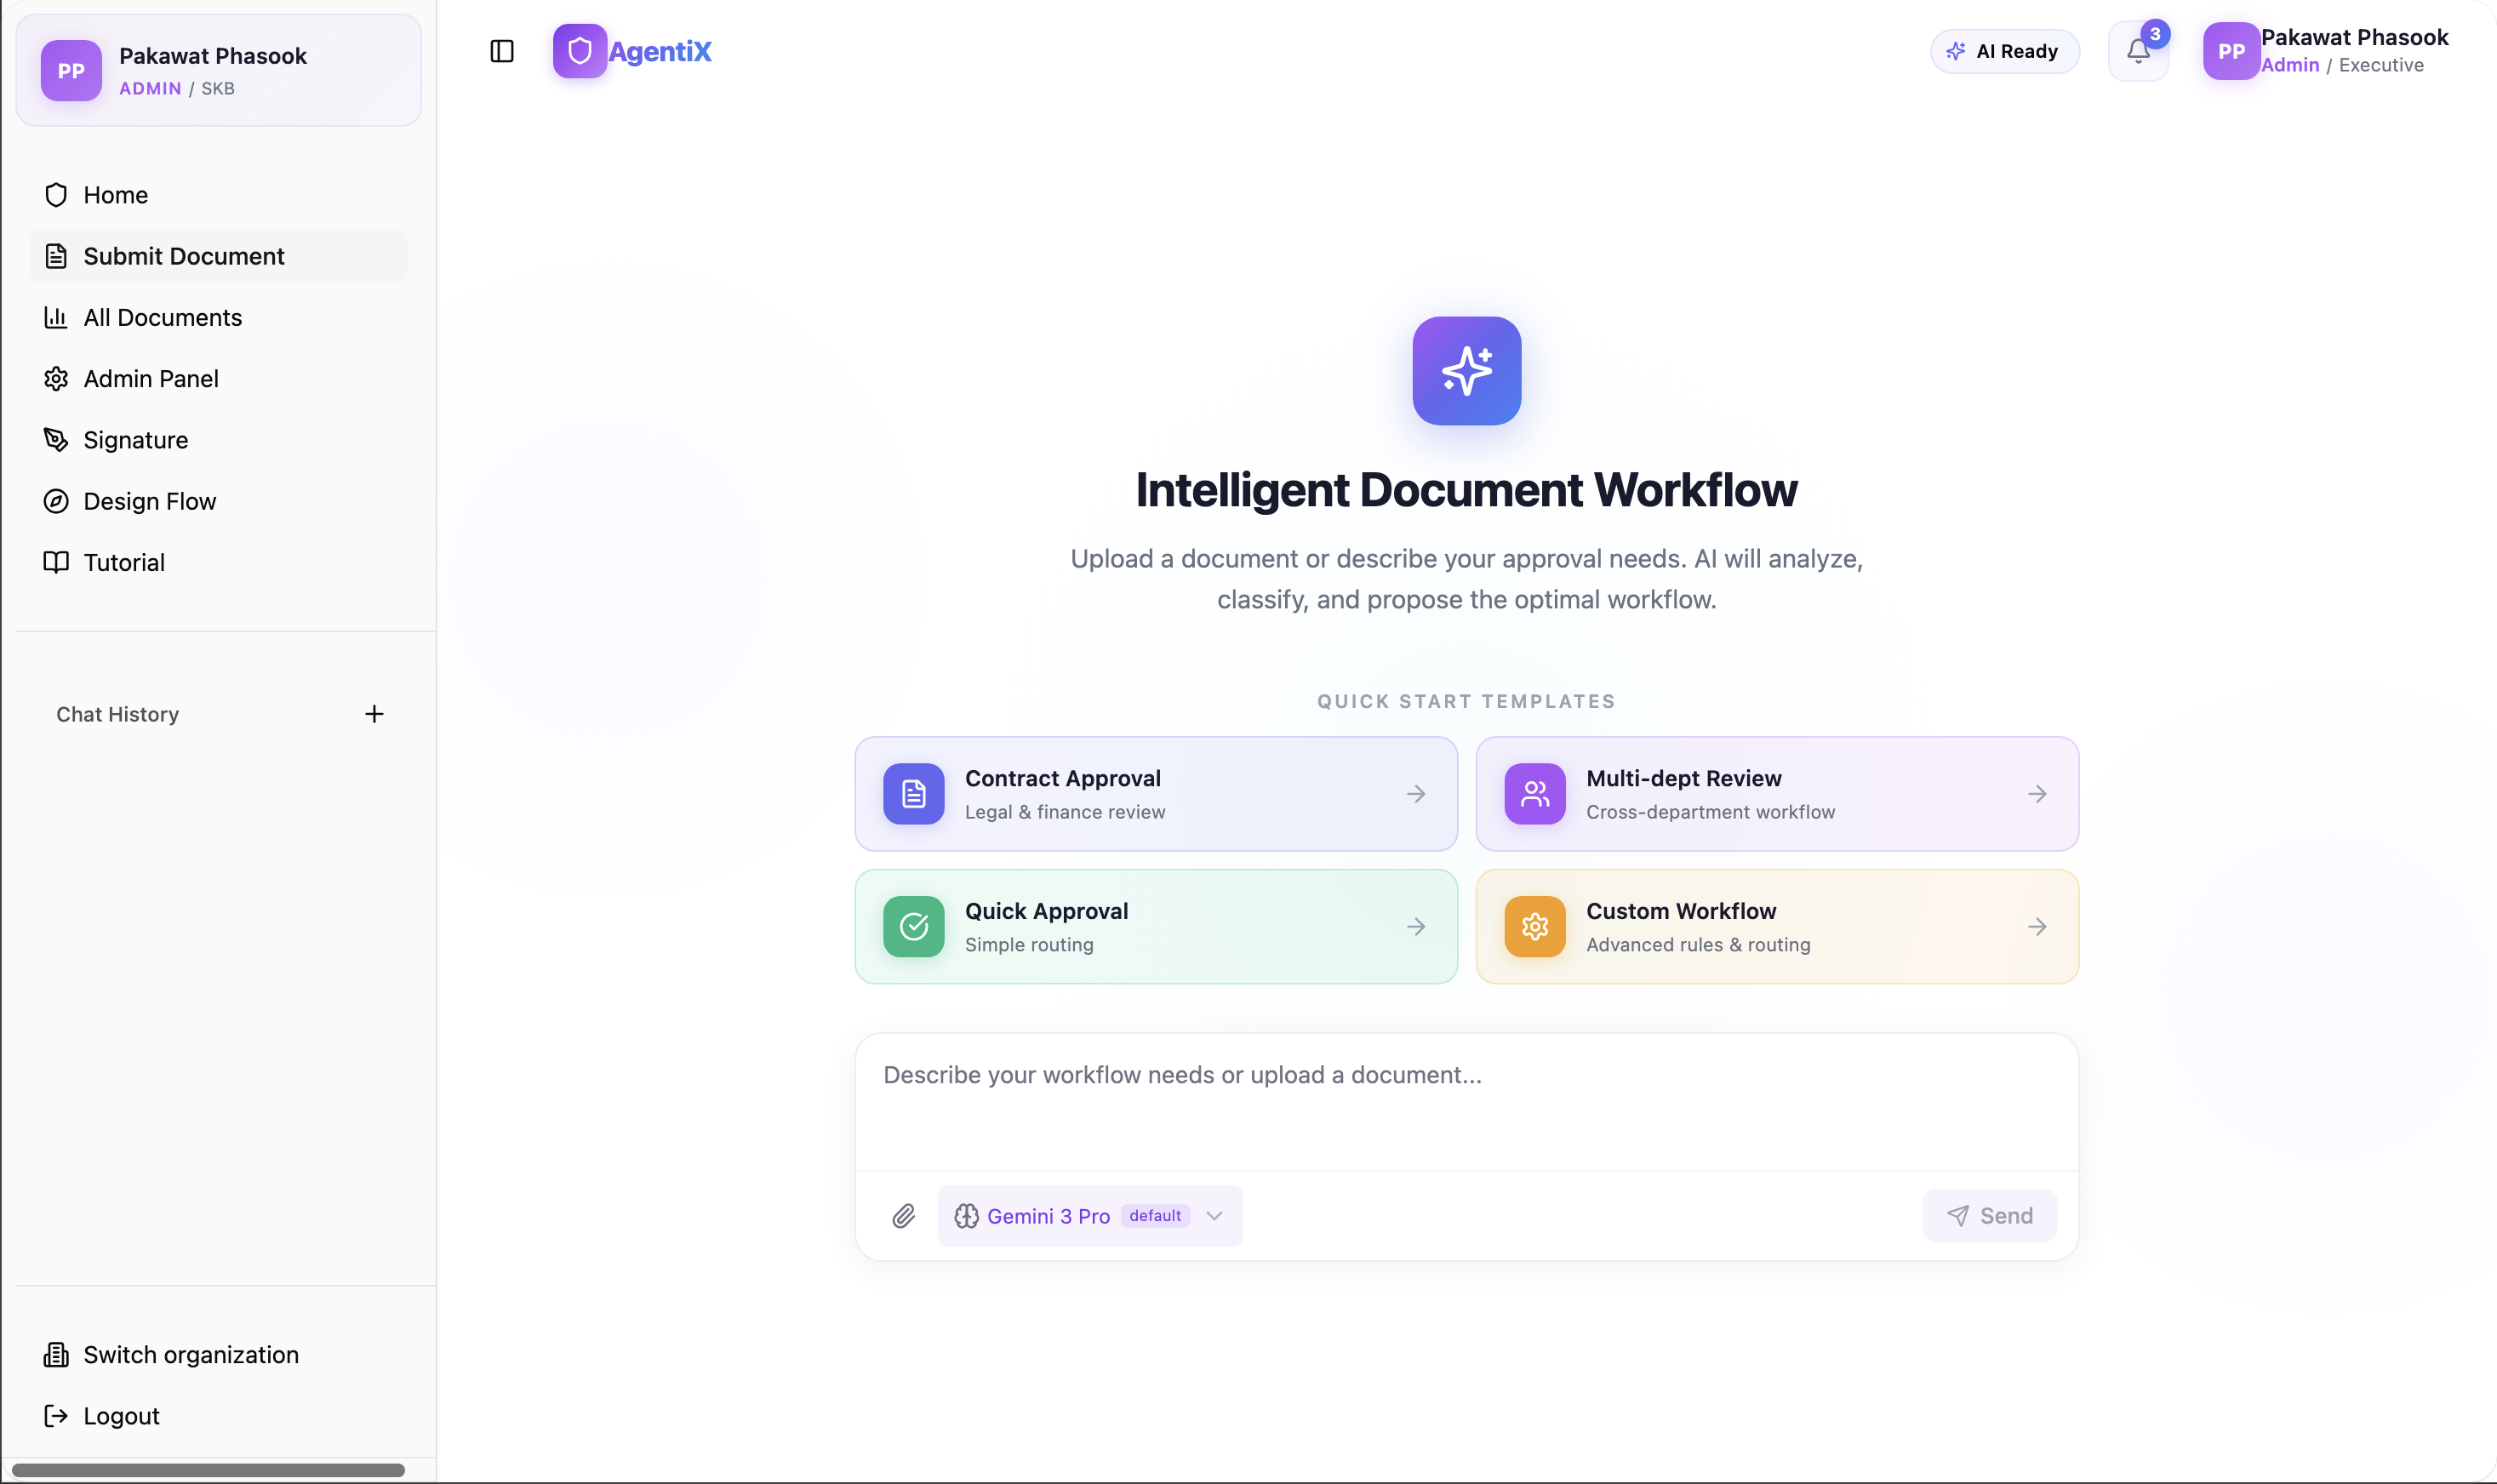
\includegraphics[width=0.85\linewidth]{image/chat_document_upload_placeholder.png}
    \caption{Submit Document interface: conversational AI-driven workflow with quick-start templates (Contract Approval, Multi-dept Review, Quick Approval, Custom Workflow) and a chat-based document submission area.}
    \label{fig:document_submission}
\end{figure}

The Document Submission interface (Figure~\ref{fig:document_submission}) represents the functional heart of AgentiX, guiding users through an intuitive, conversational workflow initiation process. Instead of static forms, the interface employs a modern chat-like paradigm combined with pre-configured templates:

\begin{itemize}
\item \textbf{Headline and Value Proposition:} ``Intelligent Document Workflow'' with supporting copy: ``Upload a document or describe your approval needs. AI will analyze, classify, and propose the optimal workflow.'' This immediately communicates the AI-driven automation capability to users.
\item \textbf{Quick-Start Templates:} Four pre-built workflow templates accelerate common use cases: ``Contract Approval'' (Legal \& Finance review), ``Multi-dept Review'' (Cross-department workflow), ``Quick Approval'' (Simple routing), and ``Custom Workflow'' (Advanced rules \& routing). Each template displays a descriptive subtitle and arrow affordance to encourage selection.
\item \textbf{Conversational Input:} A large text area prompts users to ``Describe your workflow needs or upload a document...'' The conversational framing reduces friction compared to traditional multi-step forms. Users can type natural-language requirements or upload files; the AI assistant parses both modalities.
\item \textbf{AI Model Selection:} A dropdown selector displays the active AI provider (e.g., ``Gemini 3 Pro'') with a \texttt{default} tag, allowing advanced users to manually override the model if needed. This transparency builds trust in the AI system.
\item \textbf{Chat History Panel:} A left sidebar lists previous conversations under ``Chat History,'' enabling users to reference or rerun earlier workflow configurations.
\end{itemize}

\subsubsection{Workflow Tracking and Details View}
\begin{figure}[htbp]
    \centering
    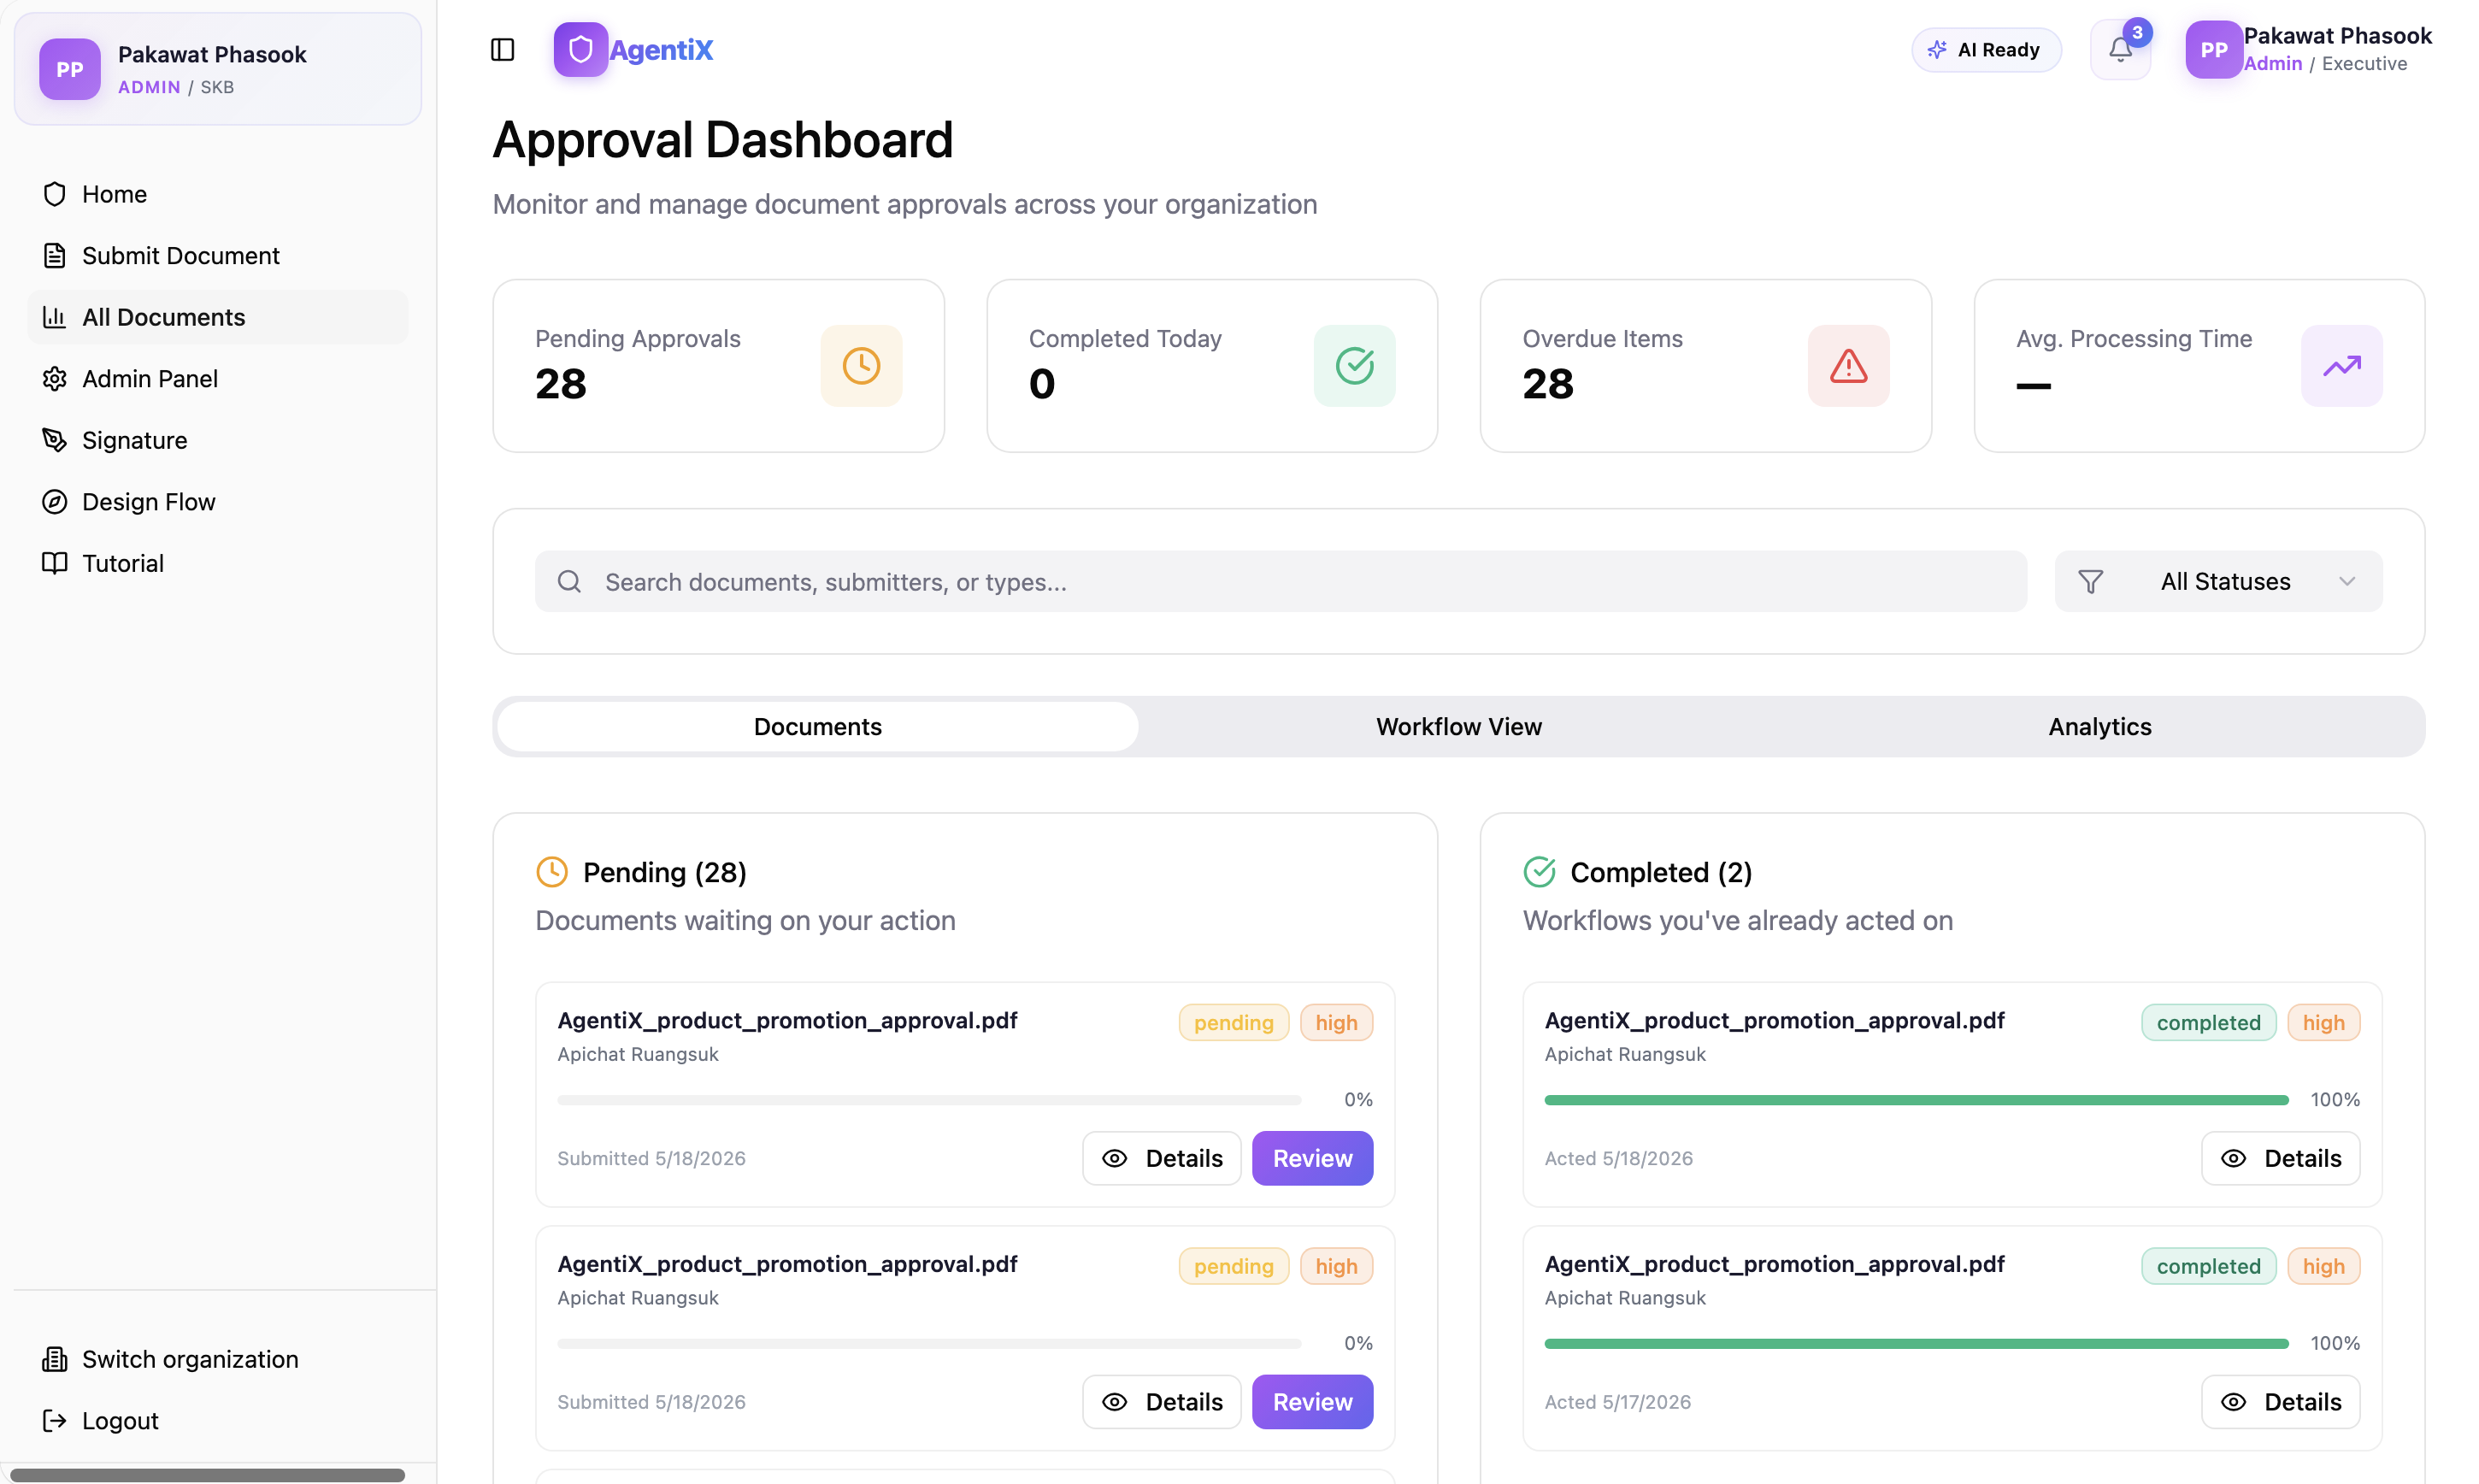
\includegraphics[width=0.85\linewidth]{image/approval_dashboard_placeholder.png}
    \caption{Workflow Details modal: displays document metadata (ID, priority, deadline), approval flow steps with status (completed/in-progress), approver information, and approval history with timestamps and comments.}
    \label{fig:workflow_details}
\end{figure}

Once a document is submitted and processing begins, users gain real-time visibility into the approval progress through the Workflow Details view (Figure~\ref{fig:workflow_details}). This modal interface surfaces critical information for both submitters and administrators:

\begin{itemize}
\item \textbf{Document Metadata:} Header displays the document title (e.g., ``Vendor Service Agreement - TechCorp'') with a ``Modify Flow'' button for workflow changes. Below, key attributes are presented: Document ID (e.g., ``DOC-001''), Priority (colour-coded, e.g., Red for ``high''), and Deadline (e.g., ``2024-01-05'').
\item \textbf{Approval Flow Visualization:} A vertical timeline shows each approval step (e.g., ``Submitted,'' ``Manager Review,'' ``Executive Approval'') with status badges. Completed steps display green checkmarks with timestamps; in-progress steps show blue indicators with assignee names (e.g., ``Ms. Anderson - VP of Operations'').
\item \textbf{Approver Information:} For each step, the interface displays the responsible approver's name and title, and their current decision status. If a decision is pending, the UI clearly indicates ``In Progress.''
\item \textbf{Approval History:} A scrollable history section records all actions chronologically, including timestamps, actor names, decisions (e.g., ``has approved the document, proceed to the next step''), and optional comments. This creates an immutable audit trail visible to all workflow participants.
\item \textbf{Action Controls:} Depending on user role, action buttons (e.g., ``View Details,'' ``Modify Flow'') appear, enabling users to inspect deeper detail, override routing decisions, or escalate for urgent approval.
\end{itemize}

This design ensures that submitters and approvers maintain continuous situational awareness throughout the document lifecycle, reducing uncertainty and enabling proactive escalation if workflows stall.

\vspace{1em}

\subsection{Approval Dashboard and Compilation Monitoring}

\subsubsection{Analytics and Performance Metrics Dashboard}
\begin{figure}[htbp]
    \centering
    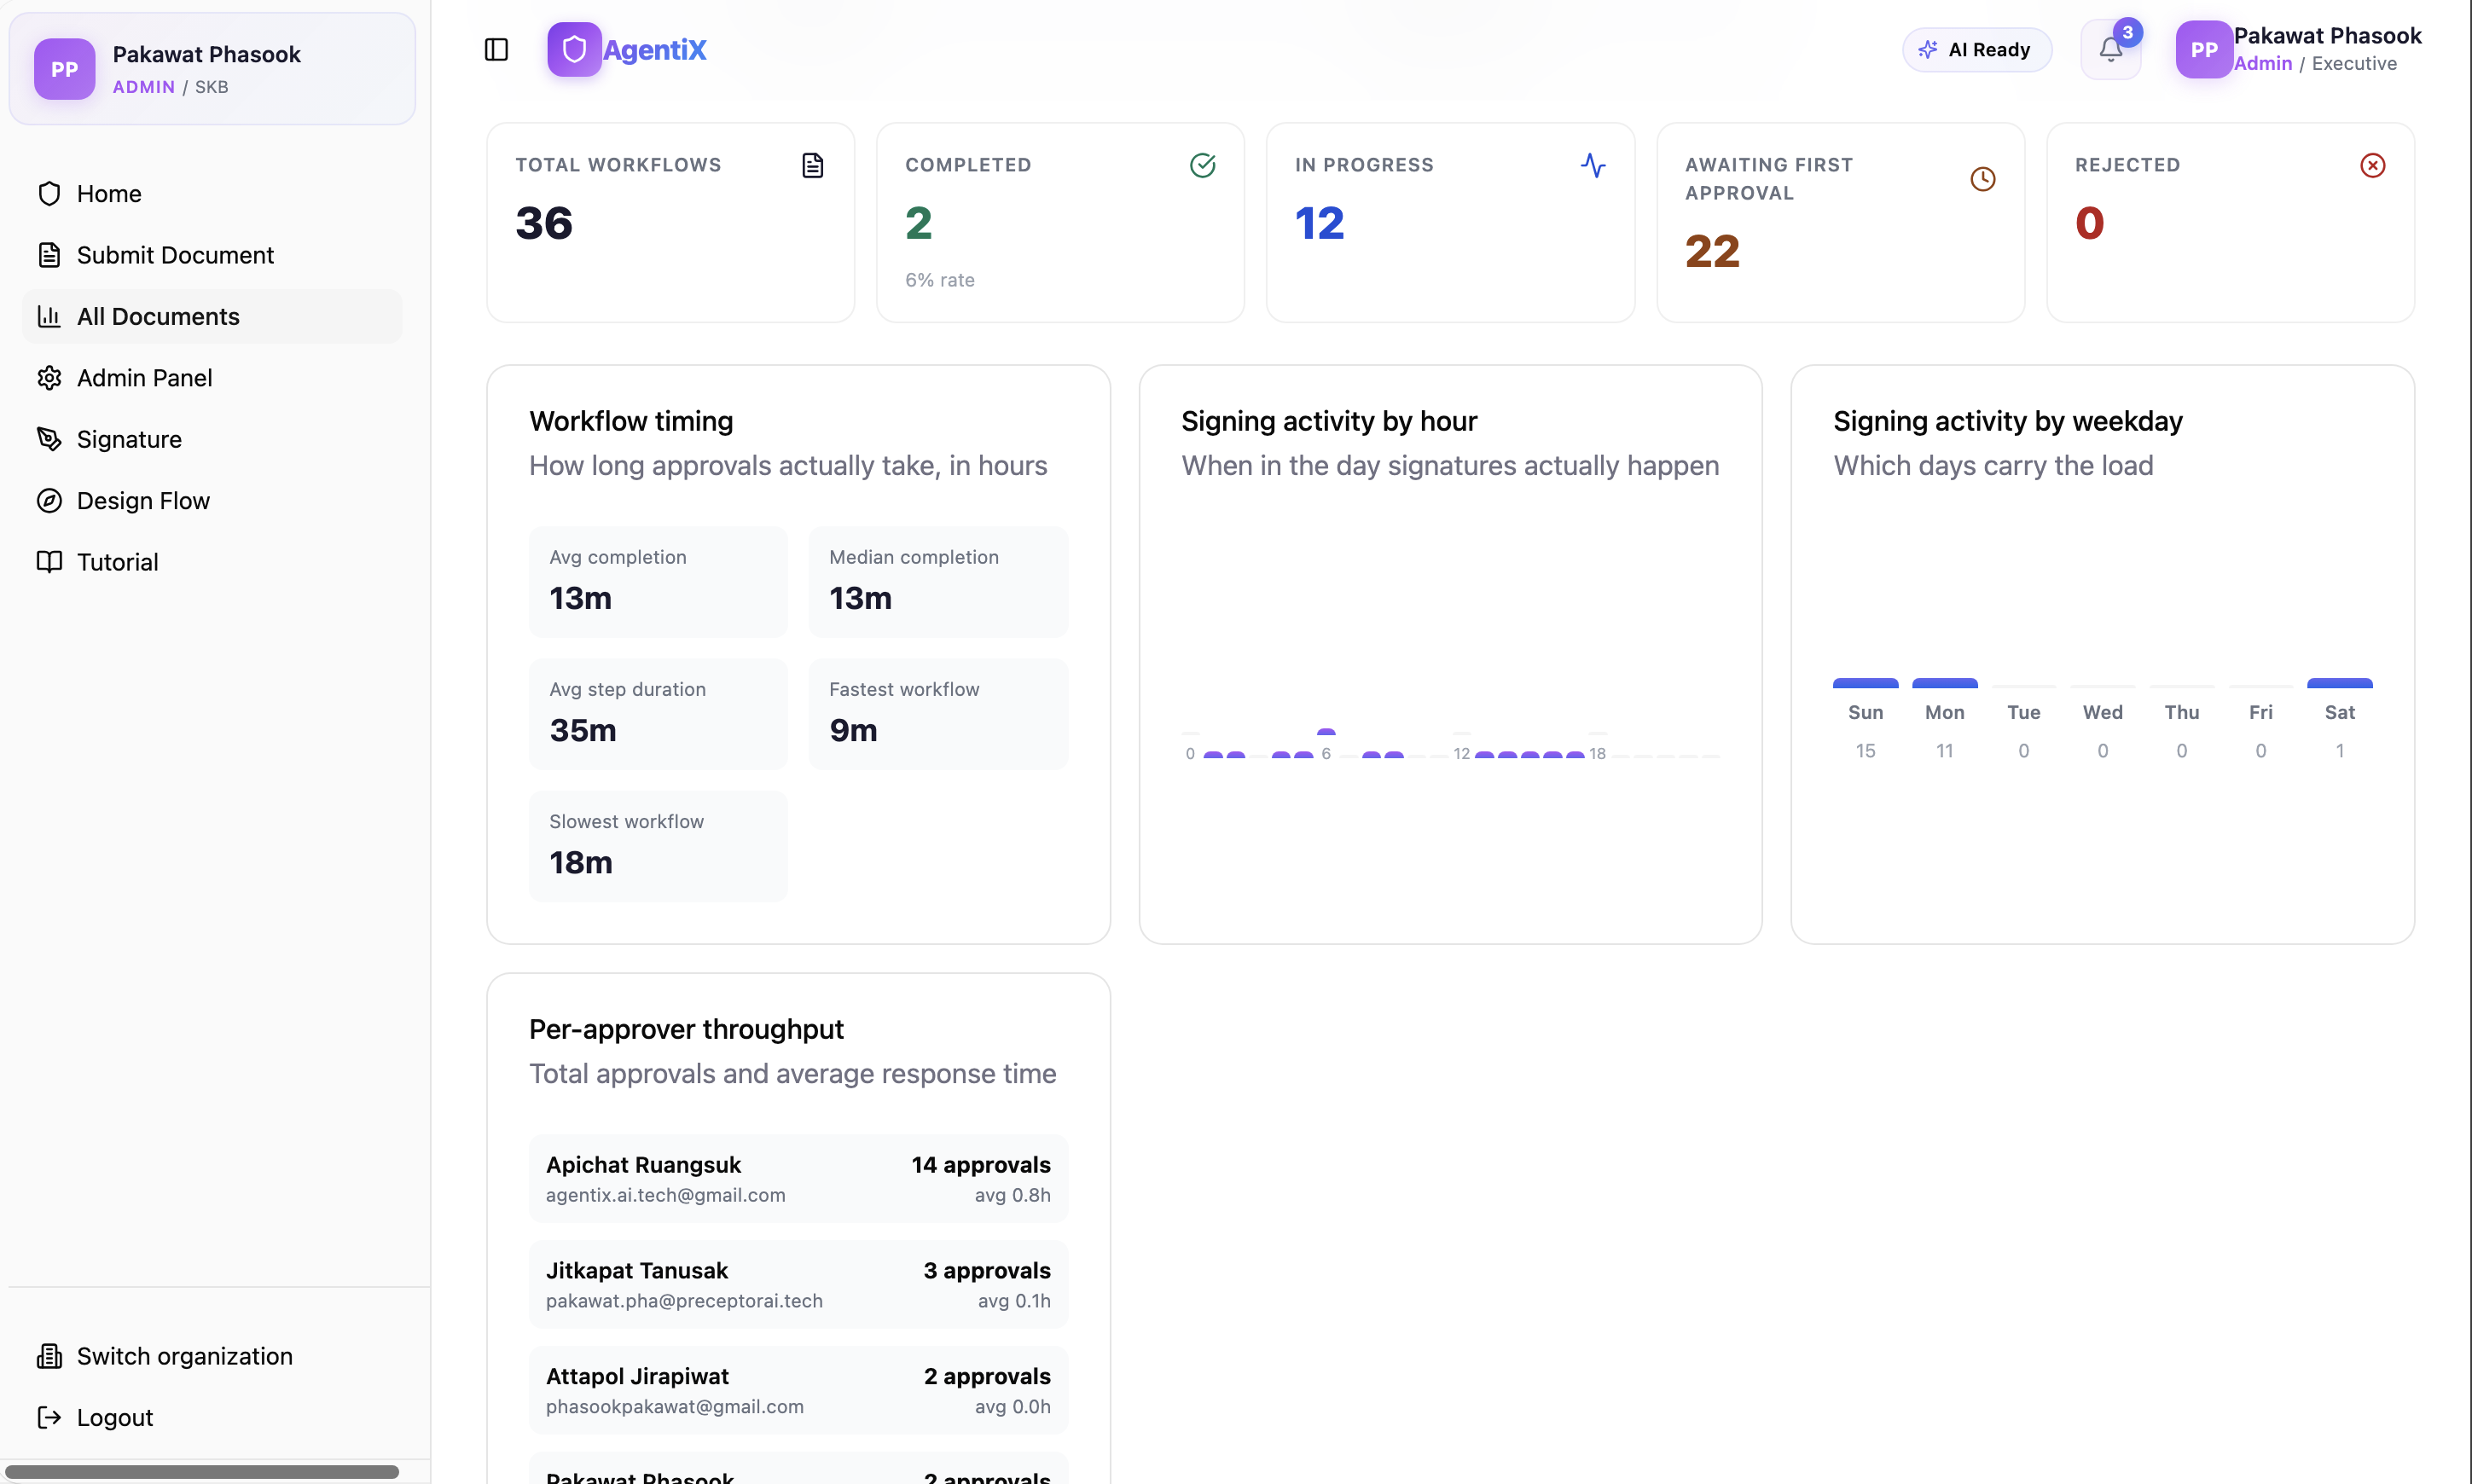
\includegraphics[width=0.9\linewidth]{image/approval_compilation_monitoring.png}
    \caption{Analytics Dashboard: displays high-level workflow metrics (total workflows, completed, in-progress, awaiting first approval, rejected), workflow timing analysis, signing activity patterns by hour and weekday, and per-approver throughput metrics.}
    \label{fig:analytics_dashboard}
\end{figure}

The Analytics Dashboard (Figure~\ref{fig:analytics_dashboard}) provides comprehensive, real-time visibility into organizational approval performance and system health. It is designed to serve both operational managers (monitoring SLAs and bottlenecks) and executives (tracking efficiency metrics):

\begin{itemize}
\item \textbf{Key Performance Indicators (KPIs):} The top row displays four critical metrics at a glance: Total Workflows (36), Completed (2, 6\% completion rate), In Progress (12), Awaiting First Approval (22), and Rejected (0). Colour-coded icons (green for completed, blue for in-progress, orange for awaiting, red for rejected) enable instant visual recognition of workflow state distribution.
\item \textbf{Workflow Timing Analysis:} A card titled ``Workflow Timing'' breaks down approval durations: Average Completion (13m), Median Completion (13m), Average Step Duration (35m), Fastest Workflow (9m), and Slowest Workflow (18m). These metrics help identify whether workflows are performing within SLAs and whether specific steps are causing delays.
\item \textbf{Signing Activity Patterns:} Two time-series charts visualize when signatures occur: ``Signing activity by hour'' shows peak signature times during the business day, while ``Signing activity by weekday'' reveals which days carry the highest load (e.g., Monday through Thursday may show higher activity than Friday). These patterns inform staffing and system capacity planning.
\item \textbf{Per-Approver Throughput:} A table lists individual approvers with their approval counts and average response times (e.g., Apichat Ruangsuk: 14 approvals, 0.8h avg; Jitkapat Tanusak: 3 approvals, 0.1h avg; Attapol Jirapiwat: 2 approvals, 0.0h avg; Pakawat Phasook: 2 approvals). This granular view enables managers to identify bottleneck approvers and redistribute workload if needed.
\end{itemize}

\subsubsection{Approval Dashboard for Document Queue Management}
\begin{figure}[htbp]
    \centering
    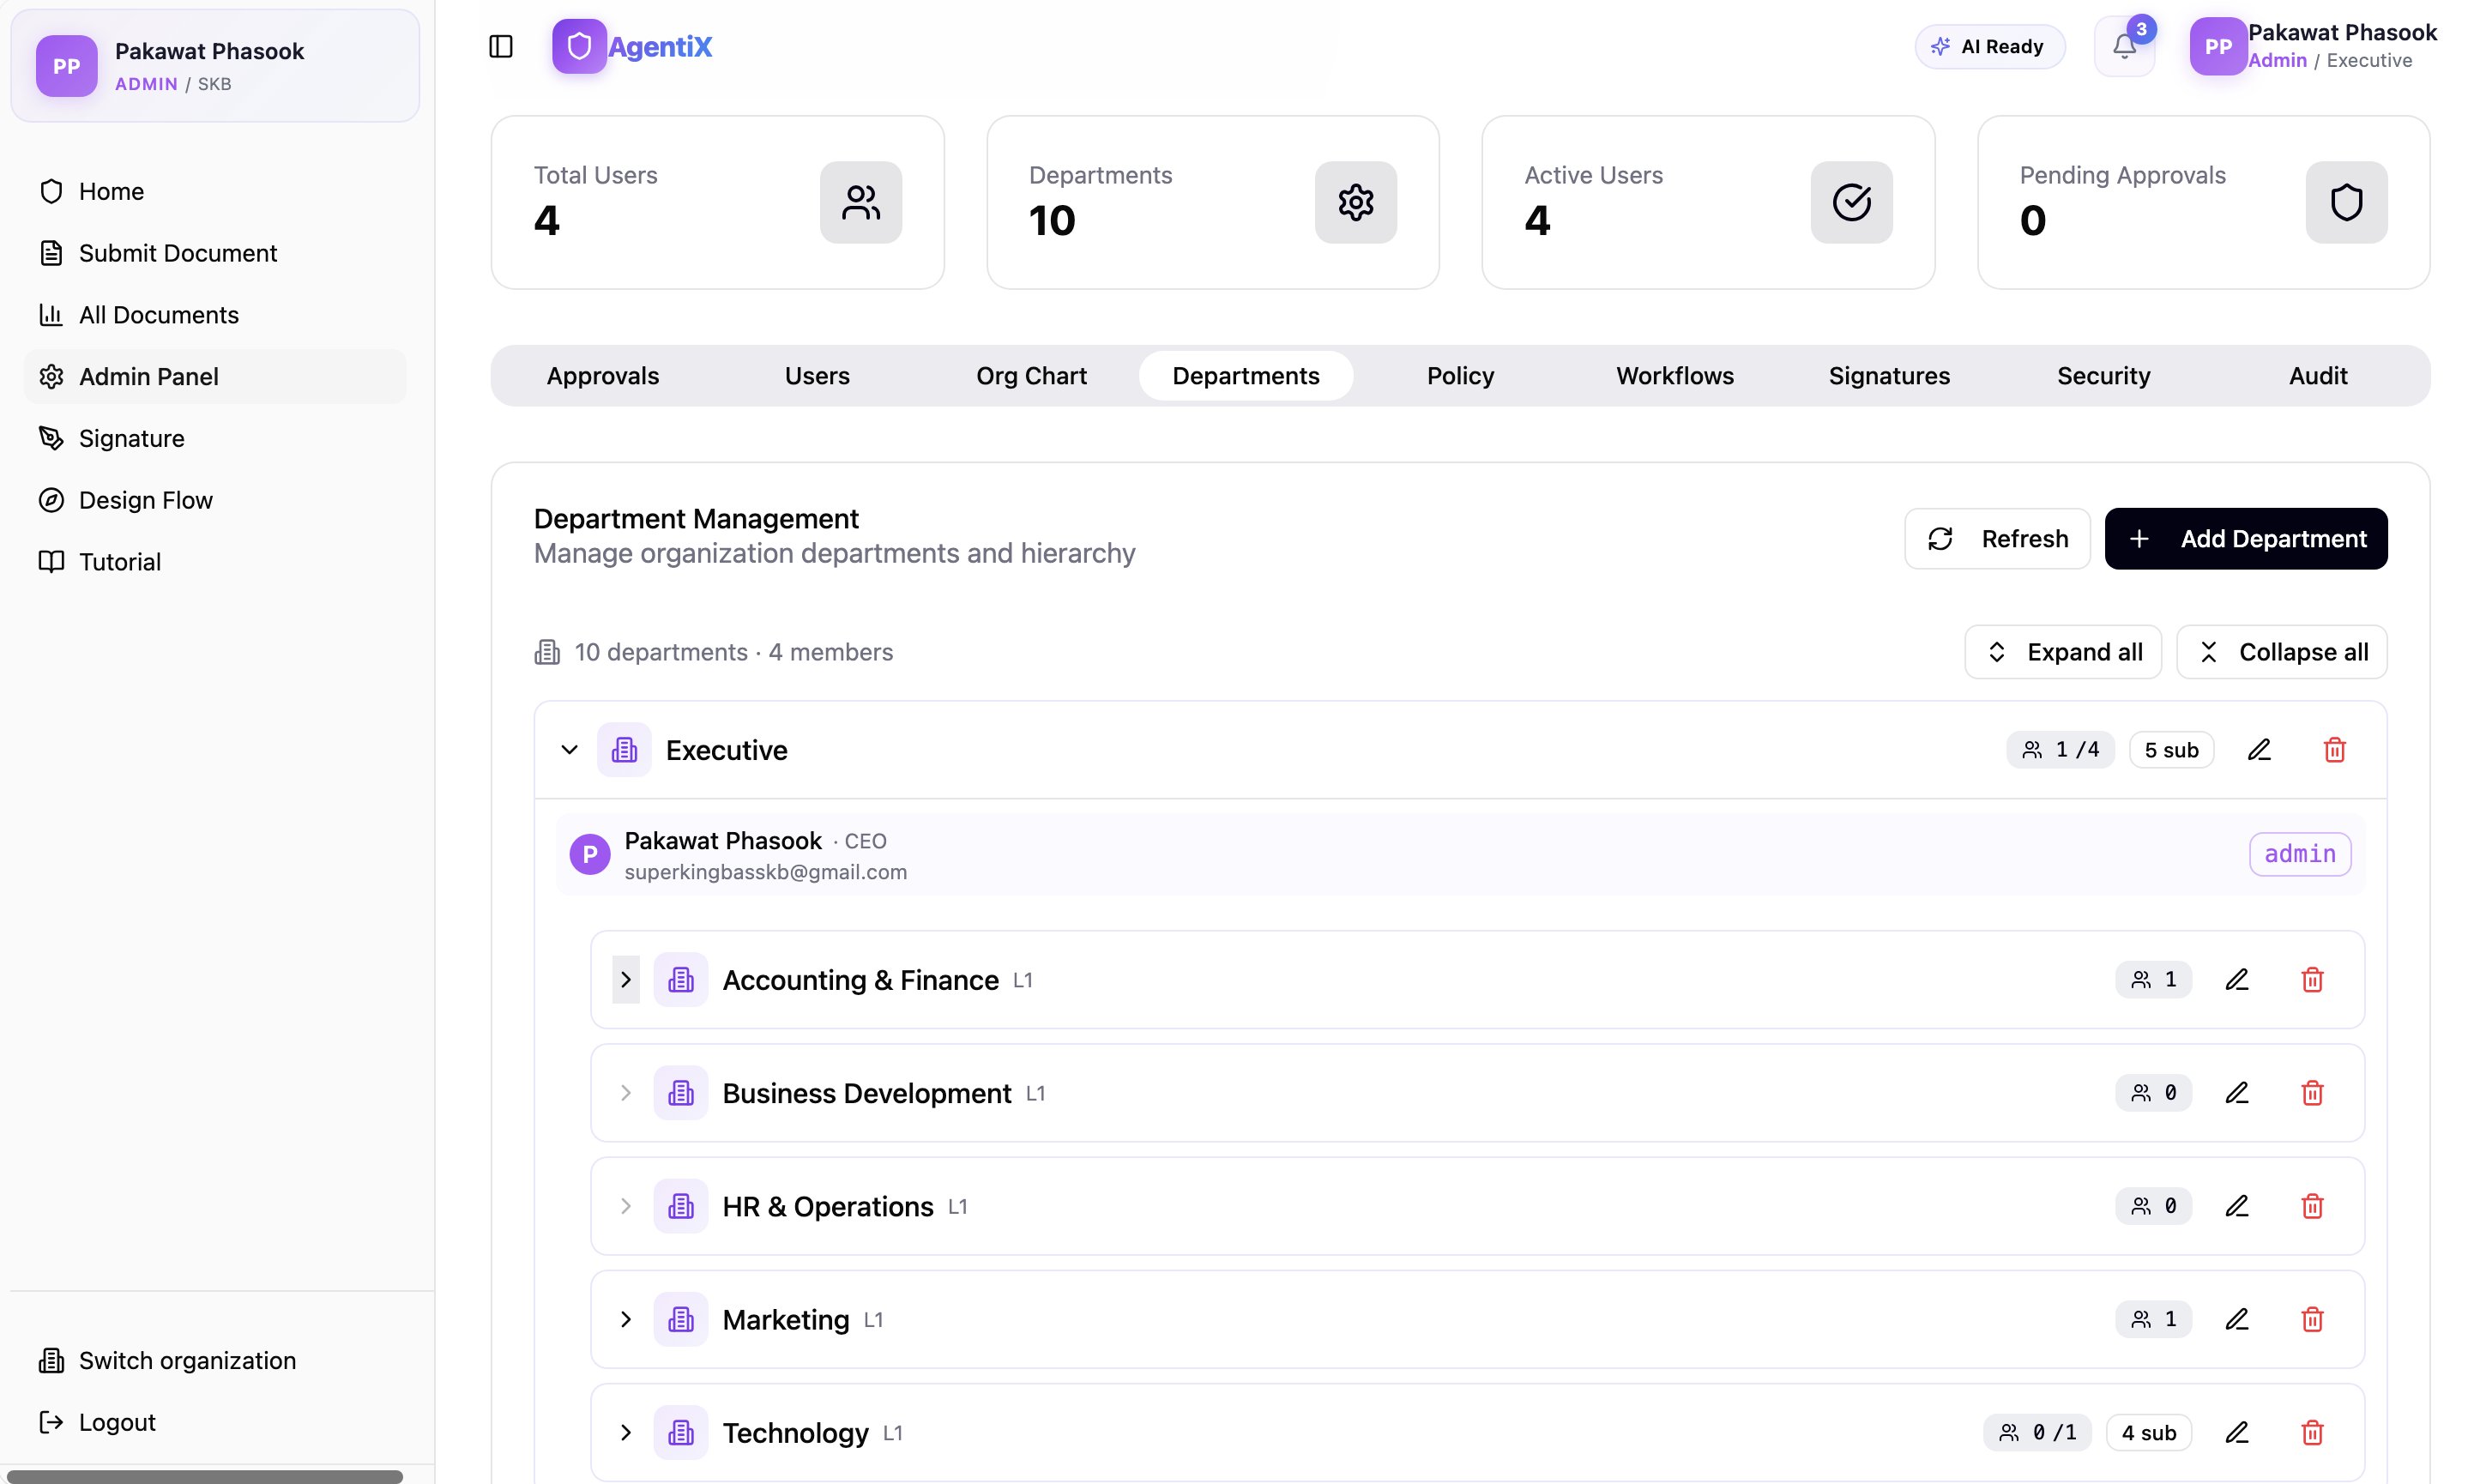
\includegraphics[width=0.9\linewidth]{image/admin_console_department.png}
    \caption{Approval Dashboard: displays pending approvals (28), completed today (0), overdue items (28), average processing time, searchable document queue with status tabs (Documents, Workflow View, Analytics), and pending/completed document lists with priority and progress tracking.}
    \label{fig:approval_dashboard}
\end{figure}

The Approval Dashboard (Figure~\ref{fig:approval_dashboard}) consolidates organizational approval tasks into a unified, actionable command center for approvers, team leads, and administrators:

\begin{itemize}
\item \textbf{Dashboard Title and Headline:} The page title ``Approval Dashboard'' with the supporting tagline ``Monitor and manage document approvals across your organization'' immediately communicates the page's purpose and scope.
\item \textbf{Top-Level Status Cards:} Four prominently displayed cards summarize the current approval state: Pending Approvals (28, with a clock icon indicating time-sensitivity), Completed Today (0, with green checkmark), Overdue Items (28, with warning triangle alert), and Average Processing Time (with upward trend icon). Colour-coding and icon usage enable quick scanning.
\item \textbf{Search and Filter Controls:} A search bar (``Search documents, submitters, or types...'') enables rapid lookup of specific workflows. A filter button (``All Statuses'') allows users to drill down by status, priority, assignee, or other dimensions, reducing noise and focusing attention on actionable items.
\item \textbf{Tabbed Views:} Three tabs organize documents by perspective: ``Documents'' (default view showing document-centric queue), ``Workflow View'' (displaying approval steps and routing logic), and ``Analytics'' (showing high-level metrics and trends). Users can switch context without leaving the dashboard.
\item \textbf{Pending Approvals Queue:} A section titled ``Pending (28)'' lists documents awaiting action. Each row displays: document filename, submitter name, status badge (``pending''), priority level (``high'', colour-coded), submission timestamp, and action buttons (``Details,'' ``Review''). The visual design uses progress bars or percentage indicators to show how far the workflow has progressed.
\item \textbf{Completed Approvals Queue:} A complementary section titled ``Completed (2)'' shows workflows that have reached terminal states. Each row displays similar metadata but with completion status and timestamps, allowing users to audit historical decisions.
\item \textbf{Workflow Progress Visualization:} Horizontal progress bars show the completion percentage for each document, providing at-a-glance status without requiring users to drill into details.
\end{itemize}

Together, these two dashboards enable organizations to operate transparently: approvers see their individual workload and response metrics; administrators and executives track system health, throughput, and bottlenecks; and all stakeholders can quickly identify and escalate documents that require attention.

\vspace{1em}

\subsection{Administration Console}

The Administration Console is a multi-faceted control centre where system administrators configure organizational structure, manage users, define approval policies, and monitor system compliance. The console employs a tabbed interface to organize distinct administrative concerns while maintaining consistent branding and navigation.

\subsubsection{Organization Structure and Department Management}
\begin{figure}[htbp]
    \centering
    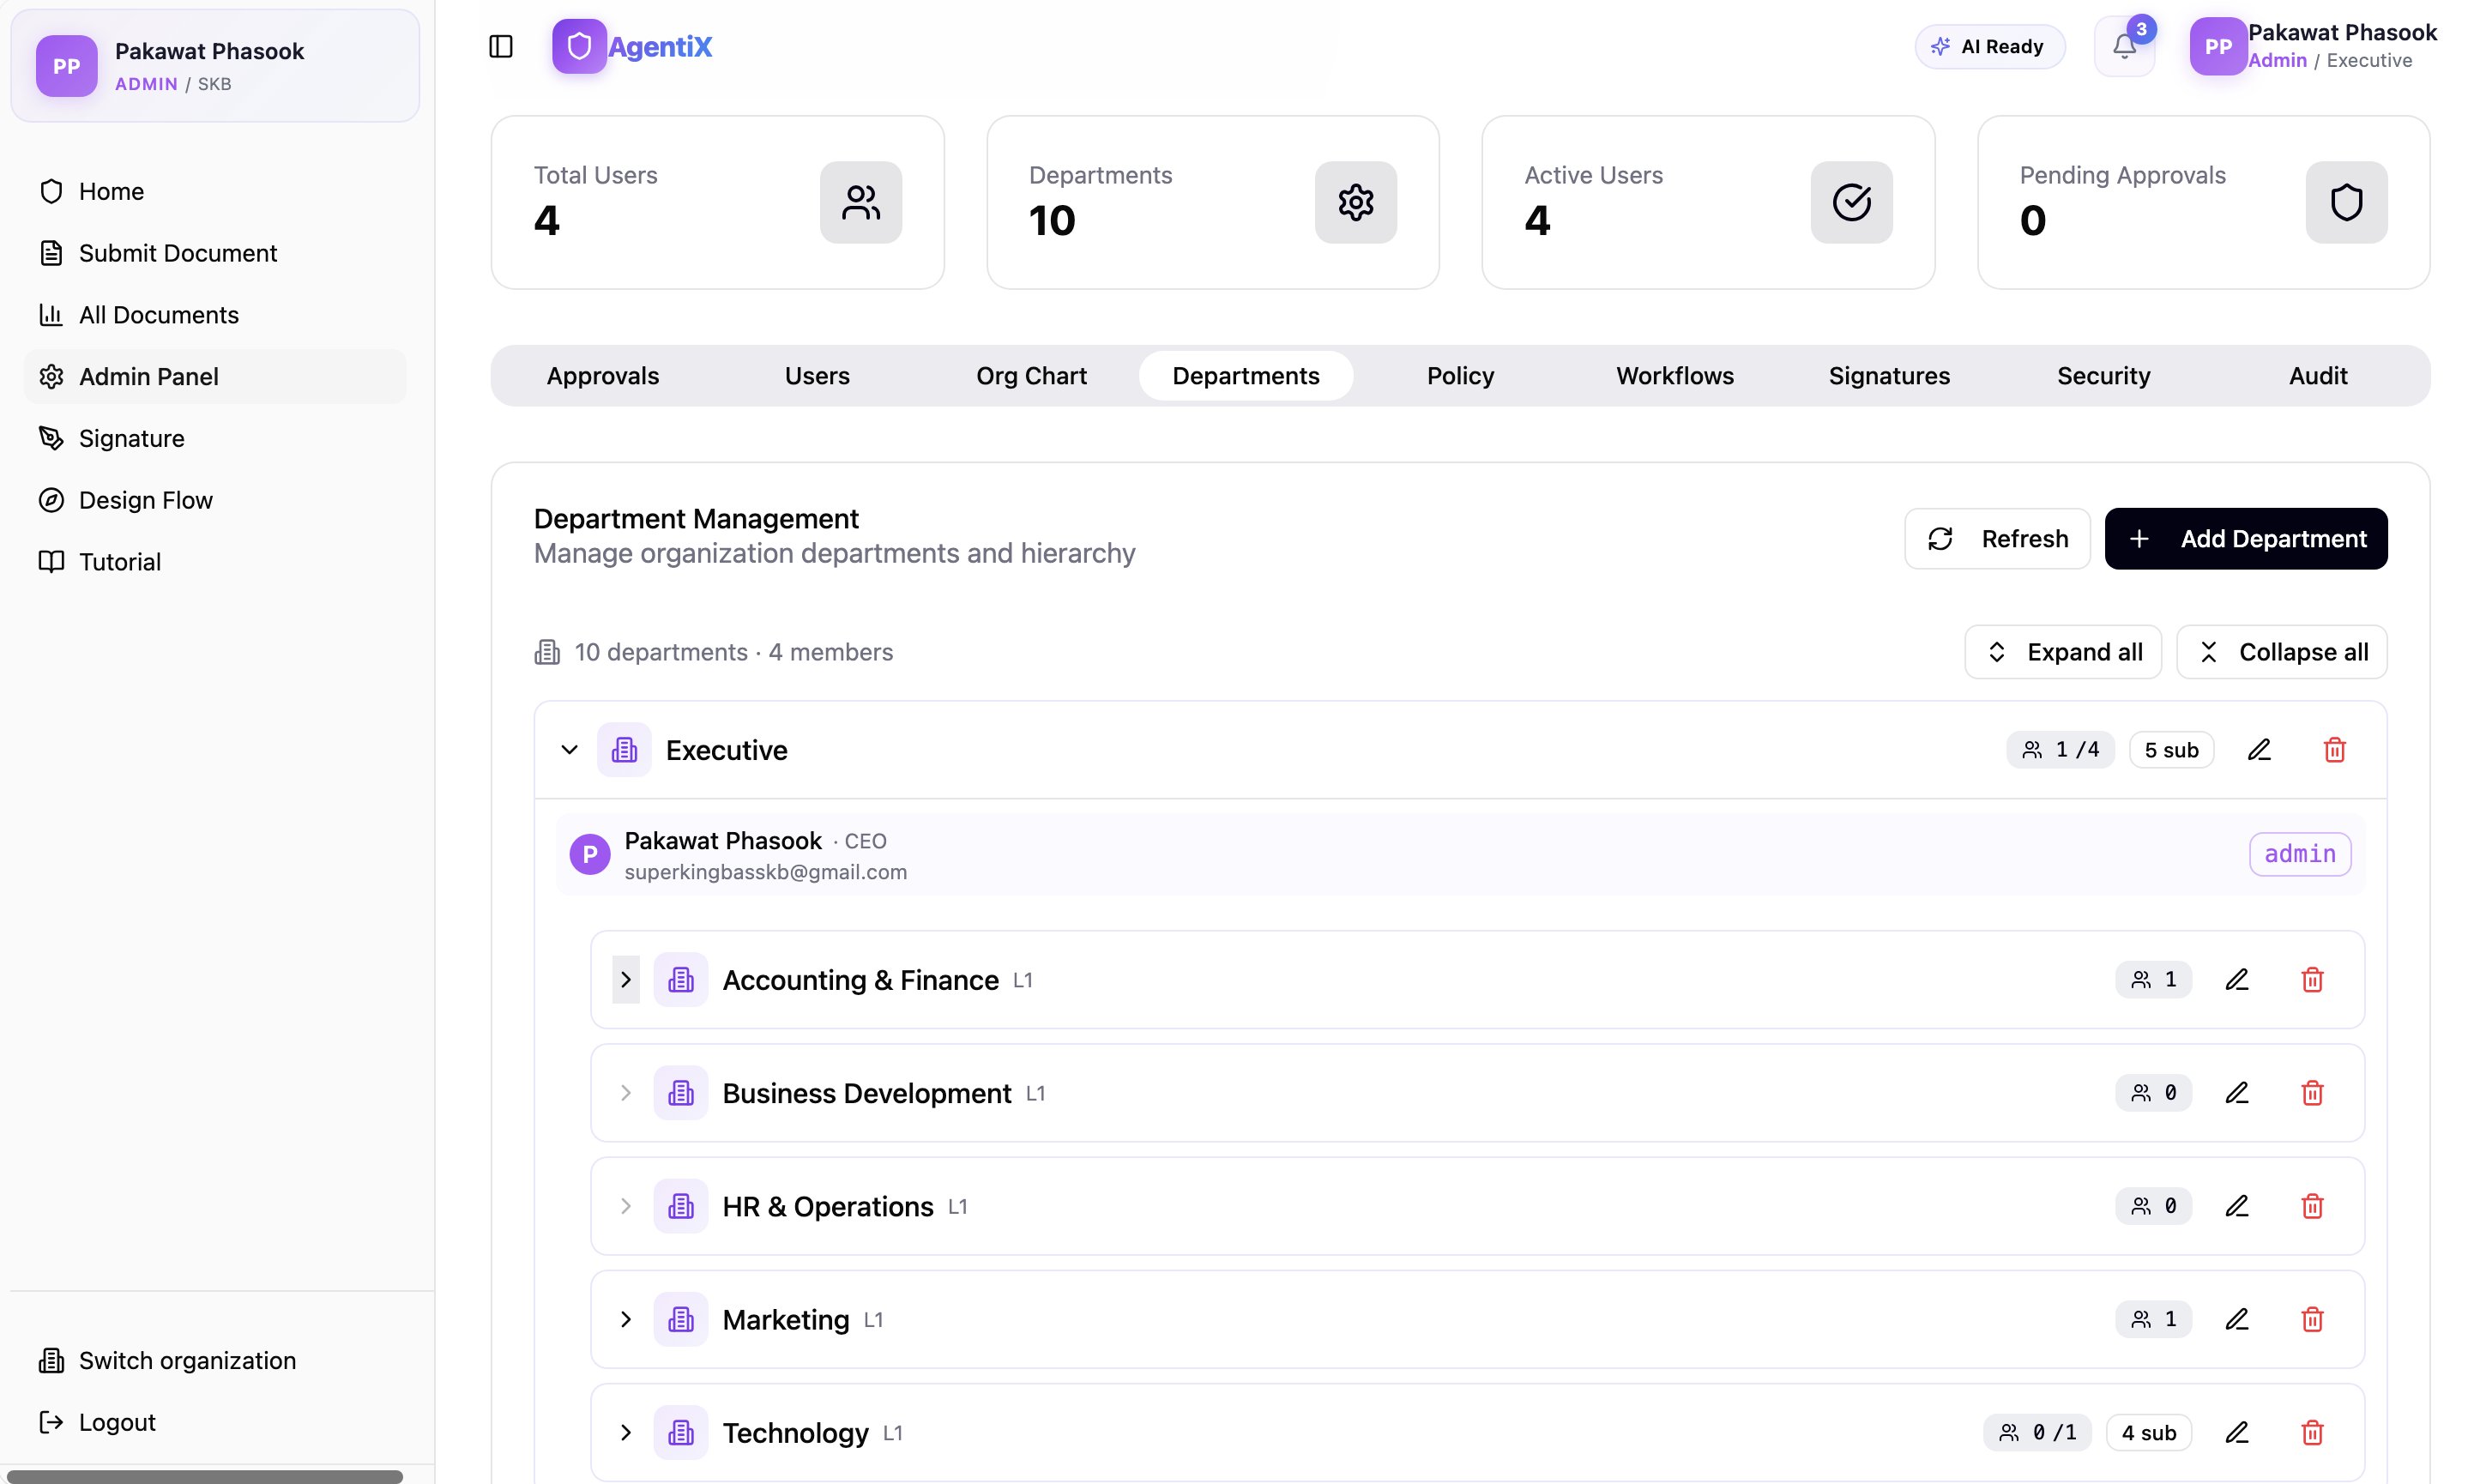
\includegraphics[width=0.9\linewidth]{image/admin_console_department.png}
    \caption{Department Management interface: displays organizational hierarchy with department cards (Executive, Accounting \& Finance, Business Development, HR \& Operations, Marketing, Technology, Product, Delivery, QA, PMO) showing member counts, sub-department relationships, and action controls (edit, delete).}
    \label{fig:department_management}
\end{figure}

The Department Management interface (Figure~\ref{fig:department_management}) enables administrators to visualize and maintain the organizational hierarchy. This hierarchical view directly influences approval routing logic, as the AI classification engine and workflow builder use this structure to propose appropriate approval chains:

\begin{itemize}
\item \textbf{Section Header:} ``Department Management'' with supporting text: ``Manage organization departments and hierarchy.'' A ``Refresh'' button enables re-sync with upstream HR systems, while an ``Add Department'' button allows manual creation of new organizational units.

\item \textbf{Department Hierarchy Display:} The interface shows a structured list of 10 departments organized under an ``Executive'' parent node. Sub-departments are visually indented to show nesting (e.g., Accounting \& Finance, Business Development, HR \& Operations, Marketing, Technology are at L1 level; Technology is shown as a parent with Product, Delivery, QA, PMO as L1 children).

\item \textbf{Department Card Details:} Each department row displays: a folder/department icon, department name, level indicator (e.g., ``L1''), member count (e.g., ``1 / 4'' showing current members vs. capacity), and action buttons (edit icon, delete icon). The compact row design allows administrators to scan the entire hierarchy quickly.

\item \textbf{Visual Indicators:} Expansion/collapse arrows allow drill-down into sub-departments. Colour-coding and icons distinguish department levels and parent-child relationships, reducing visual complexity.

\item \textbf{Bulk Actions:} ``Expand all'' and ``Collapse all'' buttons enable rapid toggling of the hierarchy view, useful when managing large organizational structures with many nesting levels.
\end{itemize}

\subsubsection{Organization Chart Upload and AI Parsing}
\begin{figure}[htbp]
    \centering
    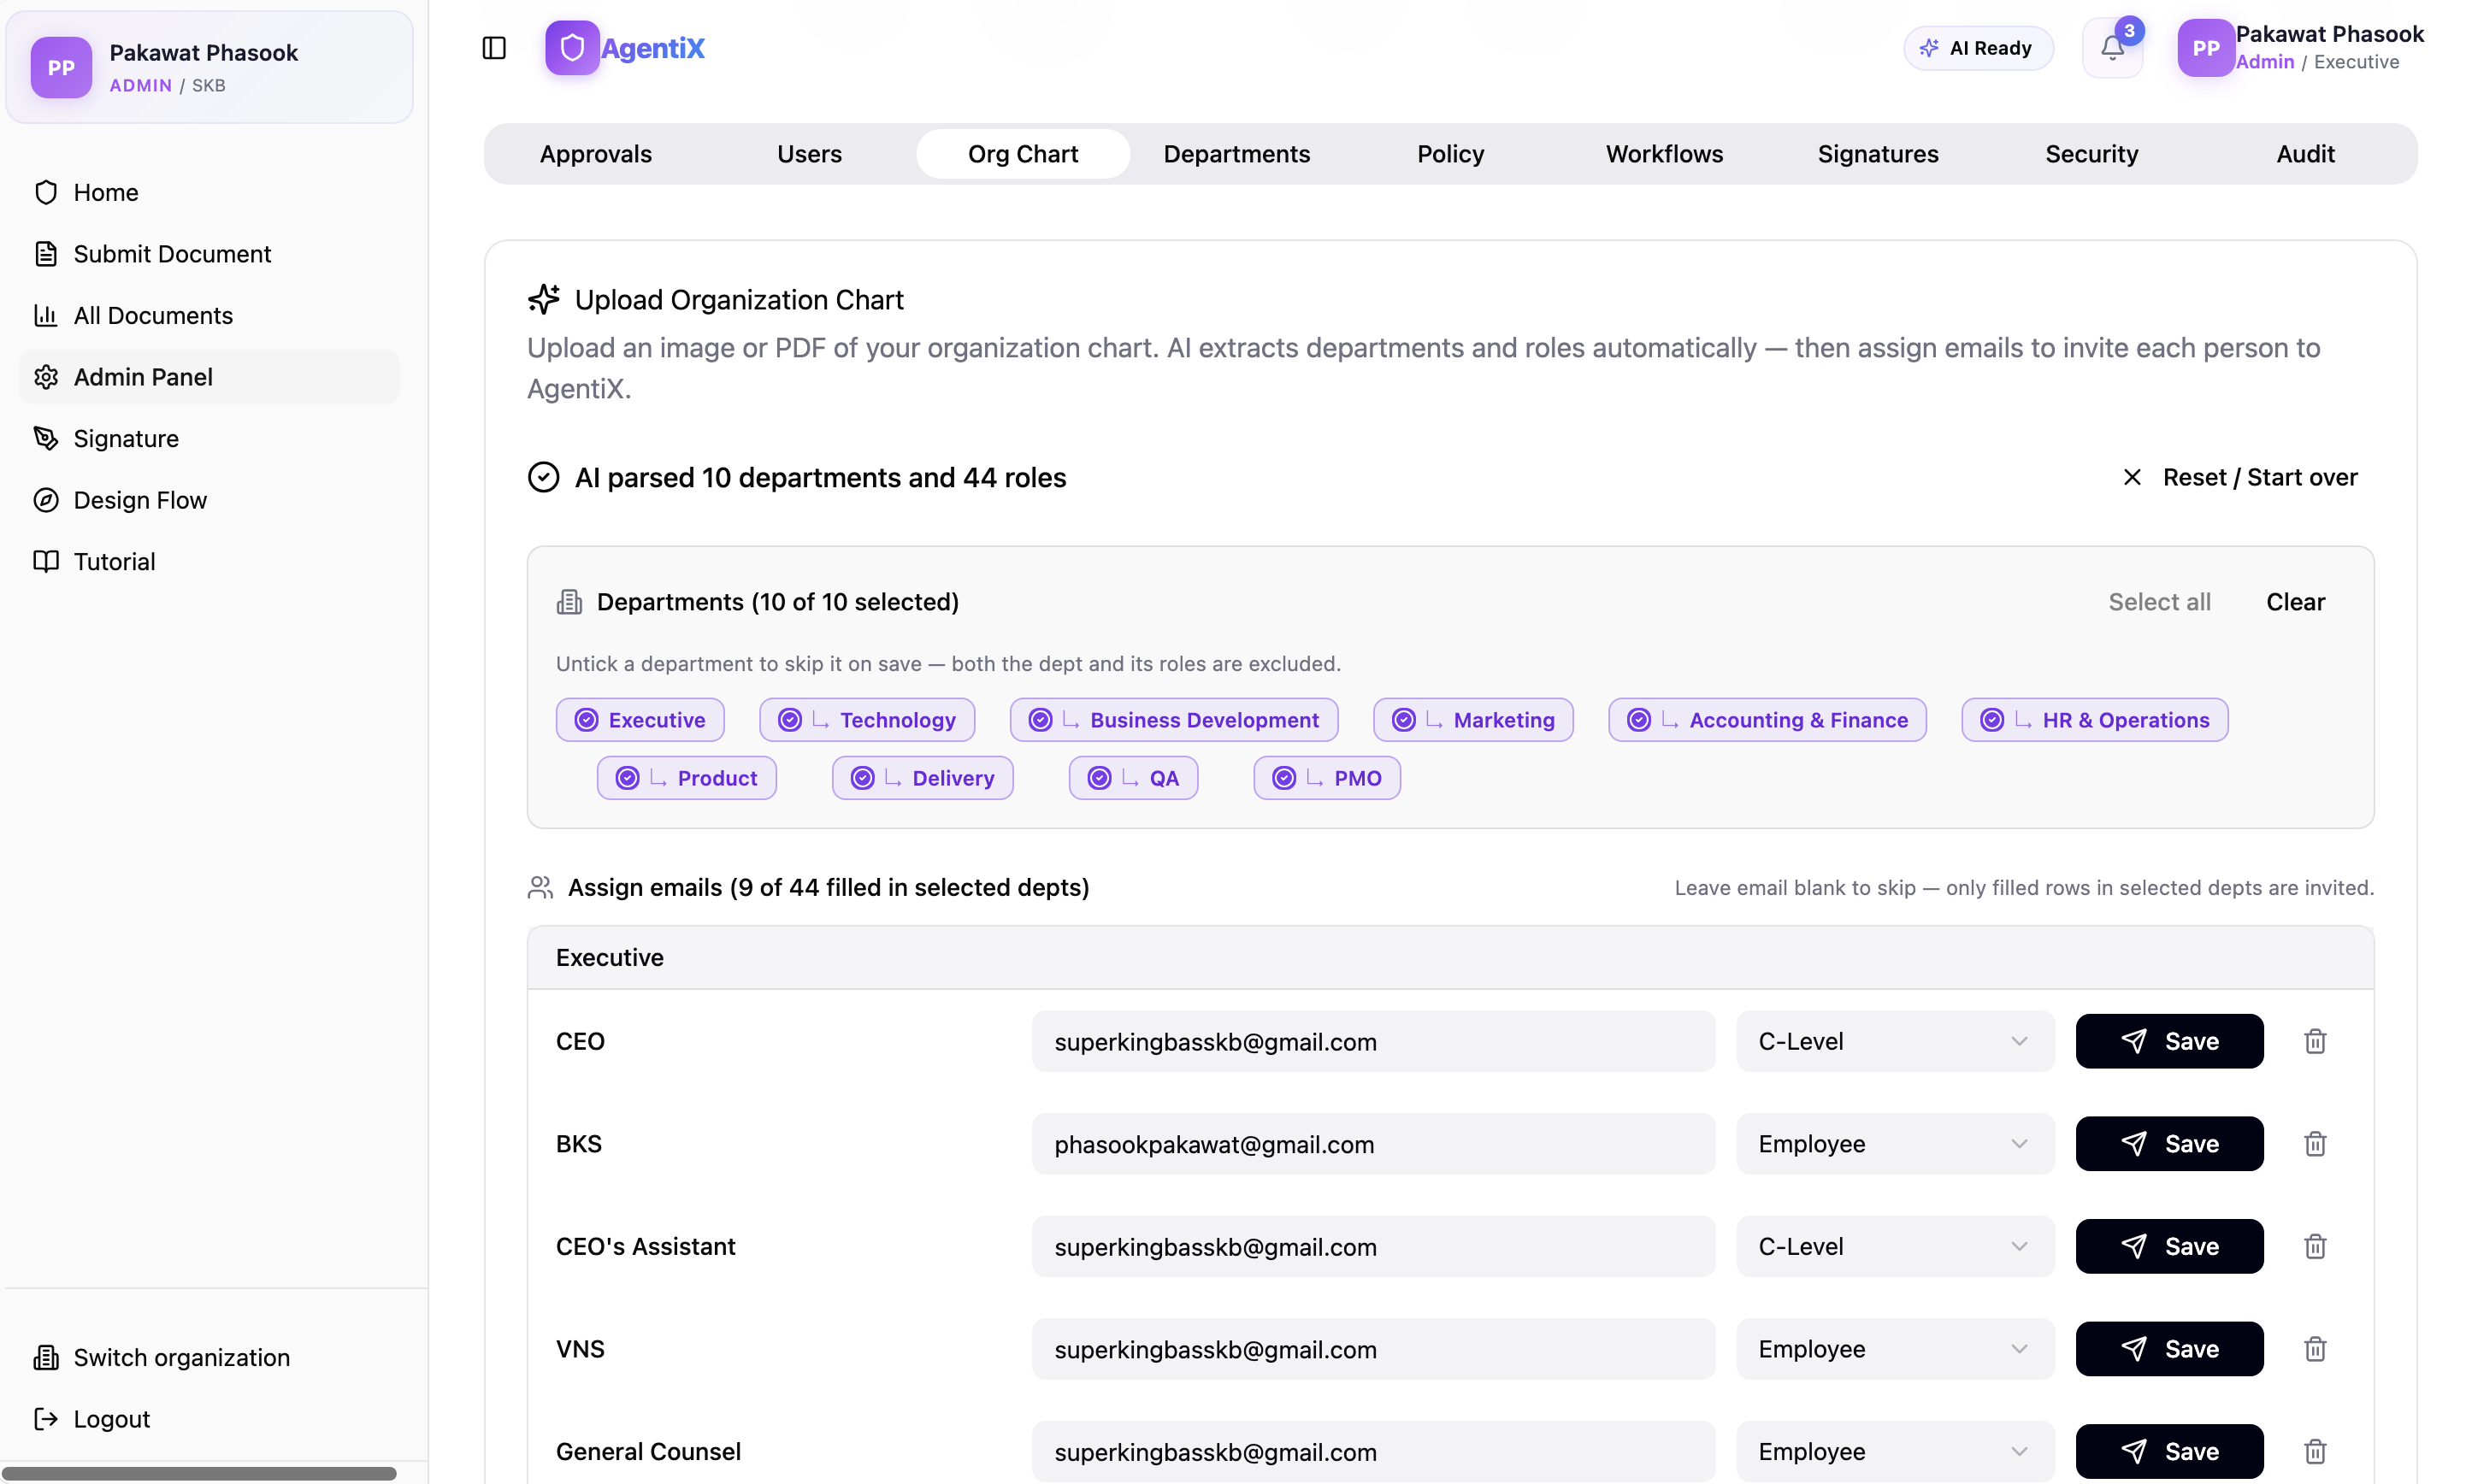
\includegraphics[width=0.9\linewidth]{image/admin_console_orgchart.png}
    \caption{Organization Chart upload interface: drag-and-drop zone for uploading org chart images/PDFs with AI parsing summary (``AI parsed 10 departments and 44 roles''), department selection checkboxes (Executive, Technology, Business Development, Marketing, Accounting \& Finance, HR \& Operations, Product, Delivery, QA, PMO), and email assignment table by department and role.}
    \label{fig:orgchart_upload}
\end{figure}

The Organization Chart Upload interface (Figure~\ref{fig:orgchart_upload}) streamlines the initial onboarding process by automating department and role extraction from visual org charts, significantly reducing manual data-entry burden:

\begin{itemize}
\item \textbf{Upload Section:} A prominent heading ``Upload Organization Chart'' with supporting text: ``Upload an image or PDF of your organization chart. AI extracts departments and roles automatically — then assign emails to invite each person to AgentiX.'' A large drag-and-drop zone displays a document icon and text: ``Drop your org chart here'' with supported formats (PNG, JPG, WebP, or PDF) listed below. A ``Choose file'' button provides an alternative file picker interface.

\item \textbf{AI Parsing Summary:} After upload, a success badge appears stating: ``AI parsed 10 departments and 44 roles,'' confirming that the extraction was successful and providing quantitative feedback on the detected organizational structure.

\item \textbf{Department Selection:} A section titled ``Departments (10 of 10 selected)'' displays colourful, rounded tag-style buttons for each extracted department (Executive, Technology, Business Development, Marketing, Accounting \& Finance, HR \& Operations, Product, Delivery, QA, PMO). Administrators can uncheck departments to exclude them from the import. A note states: ``Untick a department to skip it on save — both the dept and its roles are excluded.''

\item \textbf{Email Assignment Table:} Below the department selection, a table titled ``Assign emails (9 of 44 filled in selected depts)'' lists roles by department with email-assignment fields. Each row shows the department/role (e.g., Executive / CEO), an email input field (pre-filled or blank), a seniority dropdown (C-Level, Employee, etc.), and a ``Save'' button per row. A note reminds: ``Leave email blank to skip — only filled rows in selected depts are invited.''

\item \textbf{Progressive Disclosure:} Only a few rows are visible initially, with scrolling to reveal more entries. This prevents cognitive overload for large organizations while remaining comprehensive.
\end{itemize}

\subsubsection{User Management and Role Assignment}
\begin{figure}[htbp]
    \centering
    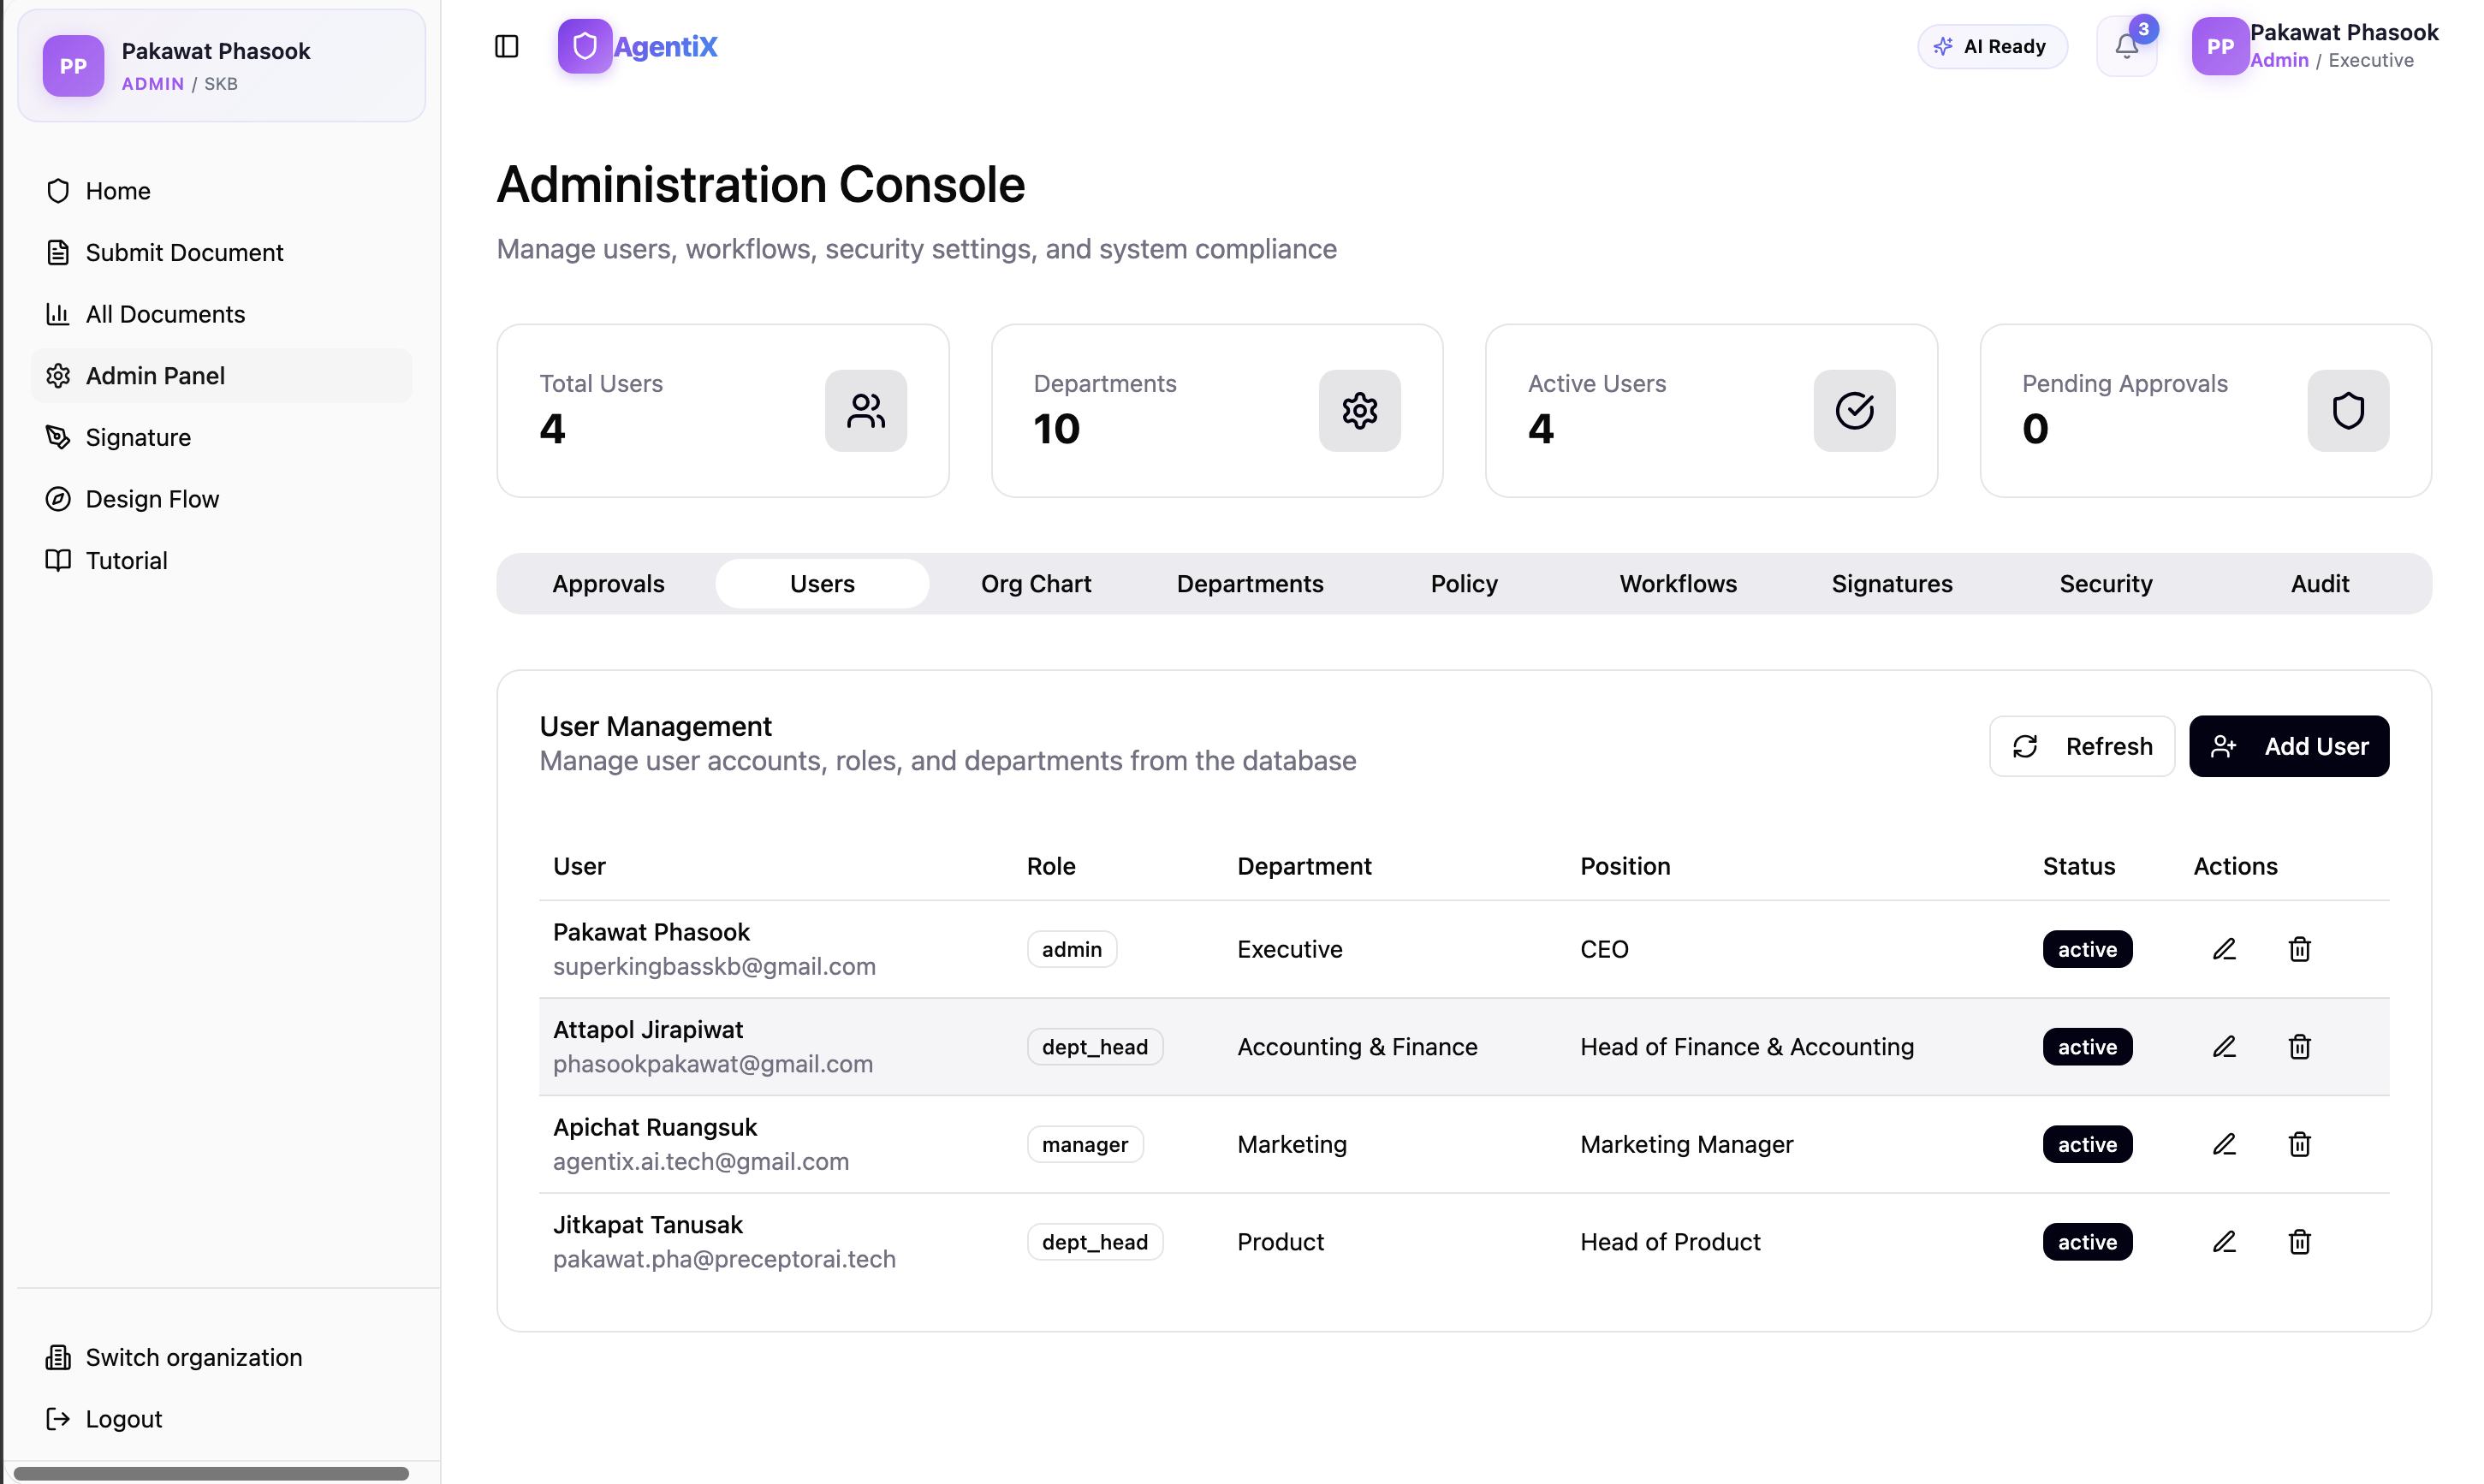
\includegraphics[width=0.9\linewidth]{image/admin_console_users.png}
    \caption{User Management interface: displays user table with columns (User, Role, Department, Position, Status, Actions), user records (Pakawat Phasook - admin/Executive/CEO, Attapol Jirapiwat - dept\_head/Accounting \& Finance, Apichat Ruangsuk - manager/Marketing, Jitkapat Tanusak - dept\_head/Product), status badges (active), and action controls (edit, delete).}
    \label{fig:user_management}
\end{figure}

The User Management interface (Figure~\ref{fig:user_management}) provides a comprehensive view of all organizational users and their roles within AgentiX. This enables administrators to grant or revoke access and adjust role-based permissions that influence approval routing:

\begin{itemize}
\item \textbf{Section Header:} ``User Management'' with supporting text: ``Manage user accounts, roles, and departments from the database.'' A ``Refresh'' button synchronizes with upstream systems, and an ``Add User'' button enables manual user creation.

\item \textbf{User Table Columns:} The table displays: User (name and email), Role (e.g., admin, dept\_head, manager), Department (organizational unit), Position (job title), Status (e.g., active badge, green), and Actions (edit and delete icons).

\item \textbf{User Records:} Example rows show:
  - Pakawat Phasook (superking basskb@gmail.com), Role: admin, Department: Executive, Position: CEO, Status: active
  - Attapol Jirapiwat (phasook pakawat@gmail.com), Role: dept\_head, Department: Accounting \& Finance, Position: Head of Finance \& Accounting, Status: active
  - Apichat Ruangsuk (agentix.ai.tech@gmail.com), Role: manager, Department: Marketing, Position: Marketing Manager, Status: active
  - Jitkapat Tanusak (pakawat.pha@preceptorial.tech), Role: dept\_head, Department: Product, Position: Head of Product, Status: active

\item \textbf{Role Semantics:} The visible roles indicate organizational hierarchy: \textit{admin} for global system administrators; \textit{dept\_head} for departmental leaders who approve documents originating in their department; and \textit{manager} for individual contributors or first-line approvers.

\item \textbf{Inline Actions:} Edit and delete icons in the Actions column allow quick modifications or removal of users without navigating to separate detail pages.
\end{itemize}

\subsubsection{Approval Policy Configuration}
\begin{figure}[htbp]
    \centering
    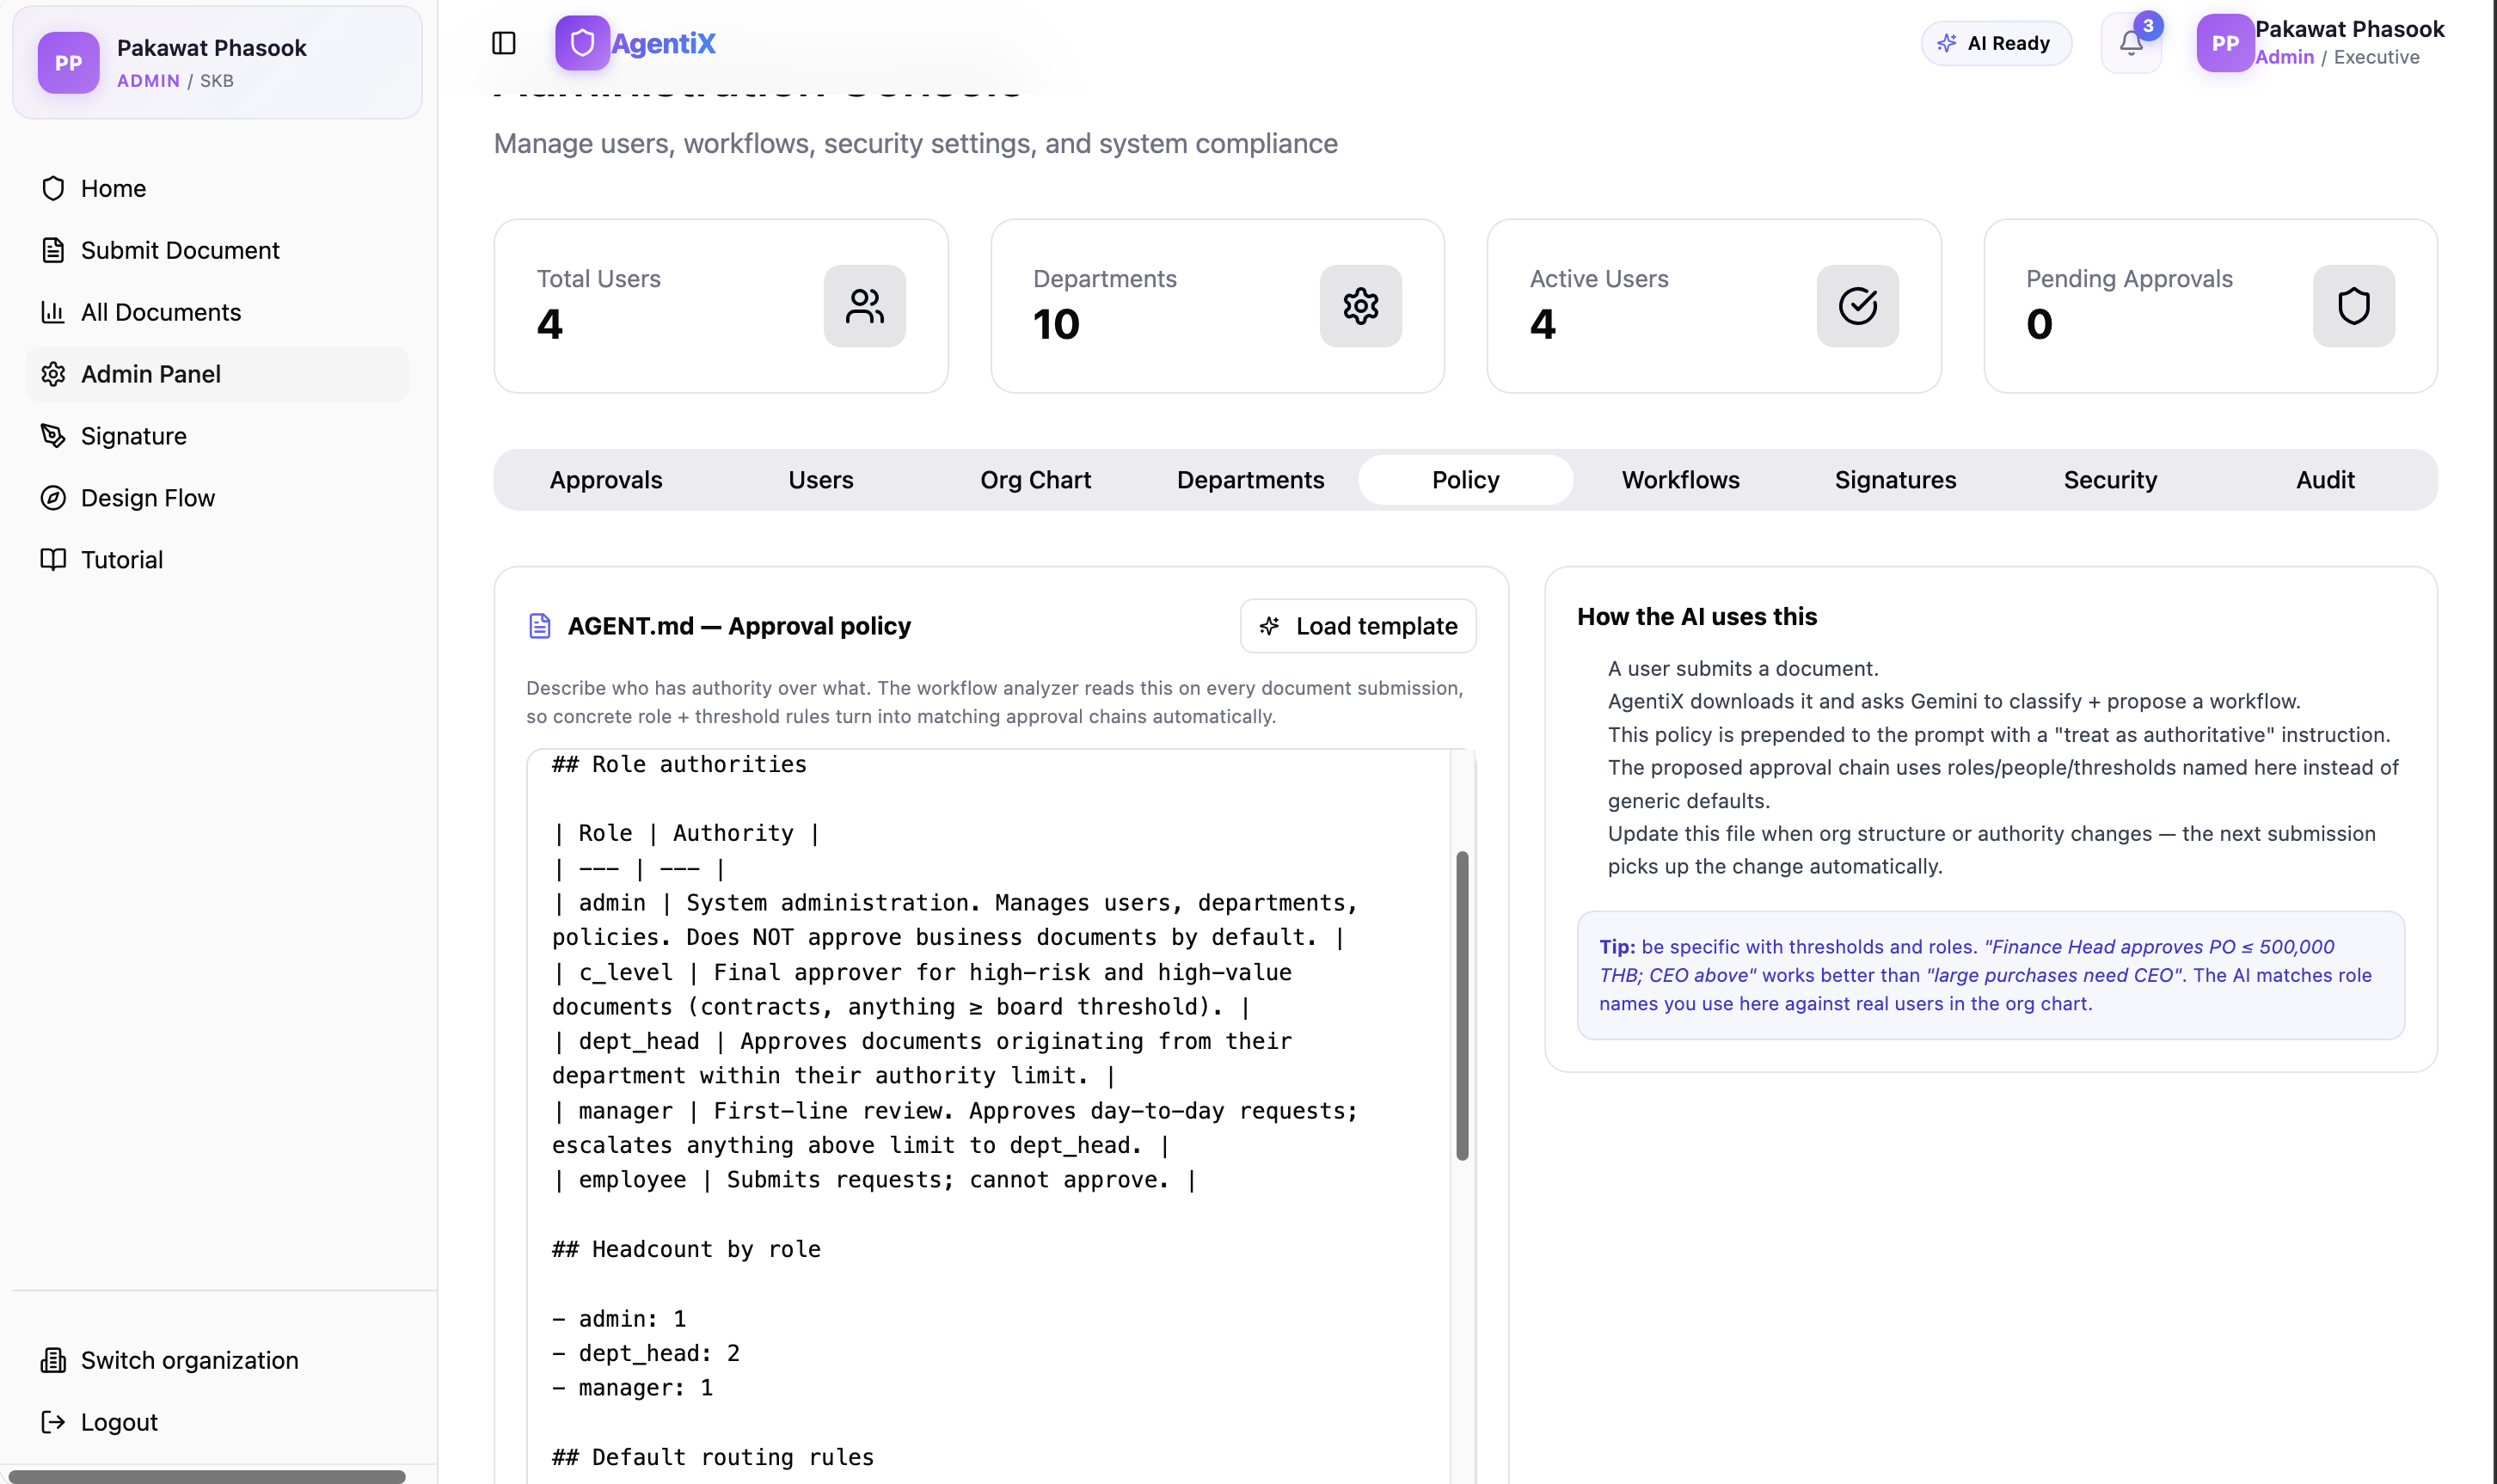
\includegraphics[width=0.9\linewidth]{image/admin_console_policy.png}
    \caption{Approval Policy editor: displays policy file (AGENT.md) with role authorities defined in structured format (admin, c\_level, dept\_head, manager, employee), role-to-threshold mappings, and a right-hand ``How the AI uses this'' panel explaining that the policy is prepended to AI prompts with a ``treat as authoritative'' instruction.}
    \label{fig:policy_configuration}
\end{figure}

The Approval Policy Configuration interface (Figure~\ref{fig:policy_configuration}) allows administrators to define role-based approval authorities and thresholds in a declarative format. This policy is automatically incorporated into the AI prompt, ensuring that the agentic classification engine makes routing decisions consistent with organizational compliance requirements:

\begin{itemize}
\item \textbf{Policy File Editor:} A code editor displays the ``AGENT.md — Approval policy'' file. The file structure defines role authorities and approval thresholds using Markdown with code-block sections:
  - ``\#\# Role authorities'' section lists roles and their approval permissions (admin, c\_level, dept\_head, manager, employee)
  - ``\#\# Headcount by role'' section enumerates role distribution (e.g., admin: 1, dept\_head: 2, manager: 1)
  - ``\#\# Default routing rules'' section specifies fallback routing if AI classification is ambiguous

\item \textbf{Example Policy Content:} The visible policy snippet shows:
  \begin{itemize}
  \item \texttt{admin | System administration. Manages users, departments, policies. Does NOT approve business documents by default.}
  \item \texttt{c\_level | Final approver for high-risk and high-value documents (contracts, anything $\geq$ board threshold).}
  \item \texttt{dept\_head | Approves documents originating from their department within their authority limit.}
  \item \texttt{manager | First-line review. Approves day-to-day requests; escalates anything above limit to dept\_head.}
  \item \texttt{employee | Submits requests; cannot approve.}
  \end{itemize}

\item \textbf{Right-Hand Guidance Panel:} A complementary panel titled ``How the AI uses this'' explains:
  ``A user submits a document. AgentiX downloads it and asks Gemini to classify + propose a workflow. This policy is prepended to the prompt with a `treat as authoritative' instruction. The proposed approval chain uses roles/people/thresholds named here instead of generic defaults. Update this file when org structure or authority changes — the next submission picks up the change automatically.''

\item \textbf{Formatting Controls:} A ``Load template'' button enables rapid policy initialization from predefined organizational patterns (e.g., startup, mid-market, enterprise).

\item \textbf{Tip Box:} A highlighted tip advises: ``Be specific with thresholds and roles. 'Finance Head approves PO above 50,000 THB; CEO above that threshold' works better than 'large purchases need CEO'. The AI matches role names you use in the org chart.''
\end{itemize}

\subsubsection{Workflow Monitoring and Audit Trail}
\begin{figure}[htbp]
    \centering
    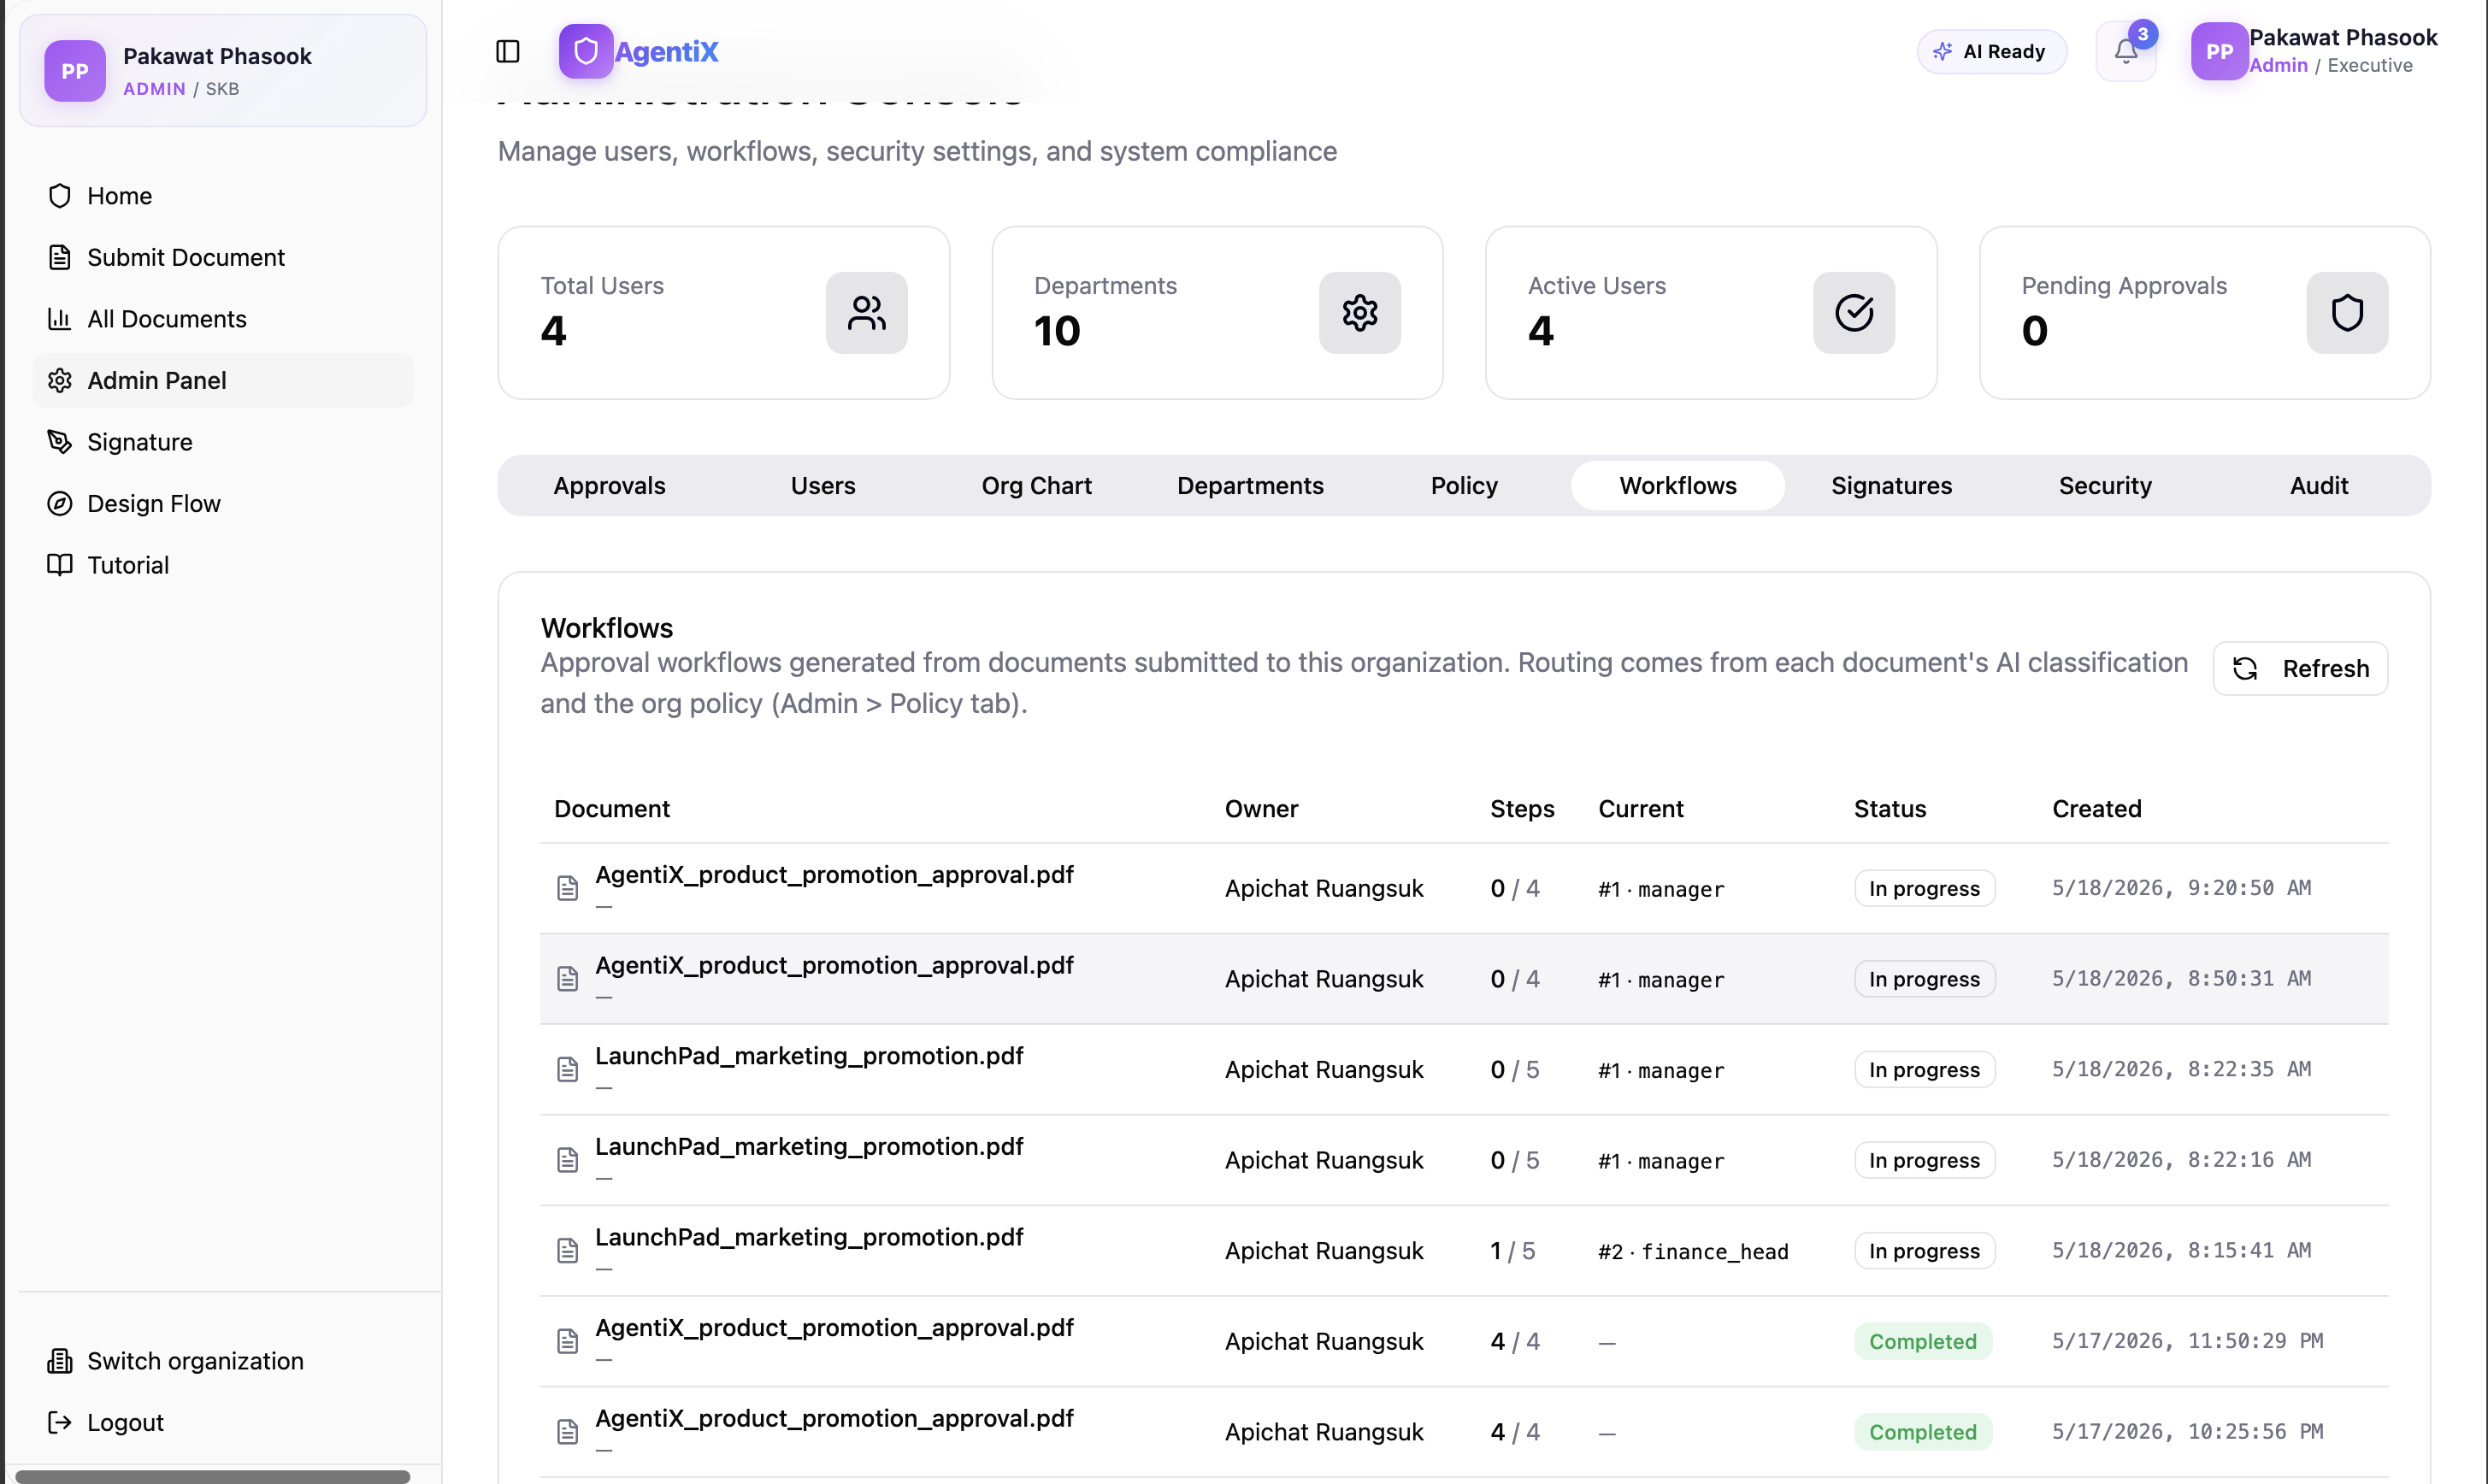
\includegraphics[width=0.9\linewidth]{image/admin_console_workflow.png}
    \caption{Workflows monitoring interface: displays active approval workflows as a data table with columns (Document, Owner, Steps, Current, Status, Created), showing document names, owners (Apichat Ruangsuk), step counts, current step indicators, status (in progress, completed), and creation timestamps.}
    \label{fig:workflow_monitoring}
\end{figure}

The Workflow Monitoring interface (Figure~\ref{fig:workflow_monitoring}) provides administrators with visibility into all active and historical workflows generated from submitted documents. This enables capacity planning, SLA monitoring, and incident investigation:

\begin{itemize}
\item \textbf{Section Header:} ``Workflows'' with supporting text: ``Approval workflows generated from documents submitted to this organization. Routing comes from each document's AI classification and the org policy (Admin $>$ Policy tab).'' A ``Refresh'' button enables manual synchronization with the backend.

\item \textbf{Workflow Table Columns:} The table displays: Document (filename), Owner (document submitter), Steps (total approval steps), Current (current step indicator), Status (in progress, completed), and Created (timestamp).

\item \textbf{Workflow Records:} Example rows show:
  - AgentiX\_product\_promotion\_approval.pdf, Apichat Ruangsuk, 0/4 steps, \#1 - manager, in progress, 5/18/2026, 9:20:50 AM
  - AgentiX\_product\_promotion\_approval.pdf, Apichat Ruangsuk, 0/4 steps, \#1 - manager, in progress, 5/18/2026, 8:50:31 AM
  - LaunchPad\_marketing\_promotion.pdf, Apichat Ruangsuk, 0/5 steps, \#1 - manager, in progress, 5/18/2026, 8:22:35 AM
  - LaunchPad\_marketing\_promotion.pdf, Apichat Ruangsuk, 0/5 steps, \#1 - manager, in progress, 5/18/2026, 8:22:16 AM
  - LaunchPad\_marketing\_promotion.pdf, Apichat Ruangsuk, 1/5 steps, \#2 - finance\_head, in progress, 5/18/2026, 8:15:41 AM
  - AgentiX\_product\_promotion\_approval.pdf, Apichat Ruangsuk, 4/4 steps, —, completed, 5/17/2026, 11:58:29 PM
  - AgentiX\_product\_promotion\_approval.pdf, Apichat Ruangsuk, 4/4 steps, —, completed, 5/17/2026, 10:25:56 PM

\item \textbf{Step Progress Indicator:} The ``Steps'' column shows progress (e.g., 0/4, 1/5, 4/4) enabling administrators to assess how far workflows have progressed. The ``Current'' column indicates which role is currently responsible (e.g., \#1 - manager, \#2 - finance\_head).

\item \textbf{Status Badges:} Status indicators use colour-coding: in progress (blue or neutral), completed (green). This allows rapid scanning of organizational throughput.

\item \textbf{Inline Details:} Administrators can click rows to drill into detailed approval history, SLA tracking, and audit trails for each workflow.
\end{itemize}

The Administration Console collectively provides the operational foundation for AgentiX. By centralizing organizational structure, user management, policy definition, and workflow monitoring, administrators can ensure that the approval system evolves with the organization and maintains compliance with business rules and regulatory requirements.

\vspace{1em}

\subsection{Signature Module}

The Signature Module is the cryptographic cornerstone of AgentiX, enabling users to capture, store, and apply digital signatures to documents with full audit traceability. The module combines biometric and cryptographic technologies to ensure that each signature is legally defensible, tamper-evident, and verifiable by external parties. The workflow progresses through capture, verification, and embedding phases.

\subsubsection{Signature Capture and Cropping Interface}
\begin{figure}[htbp]
    \centering
    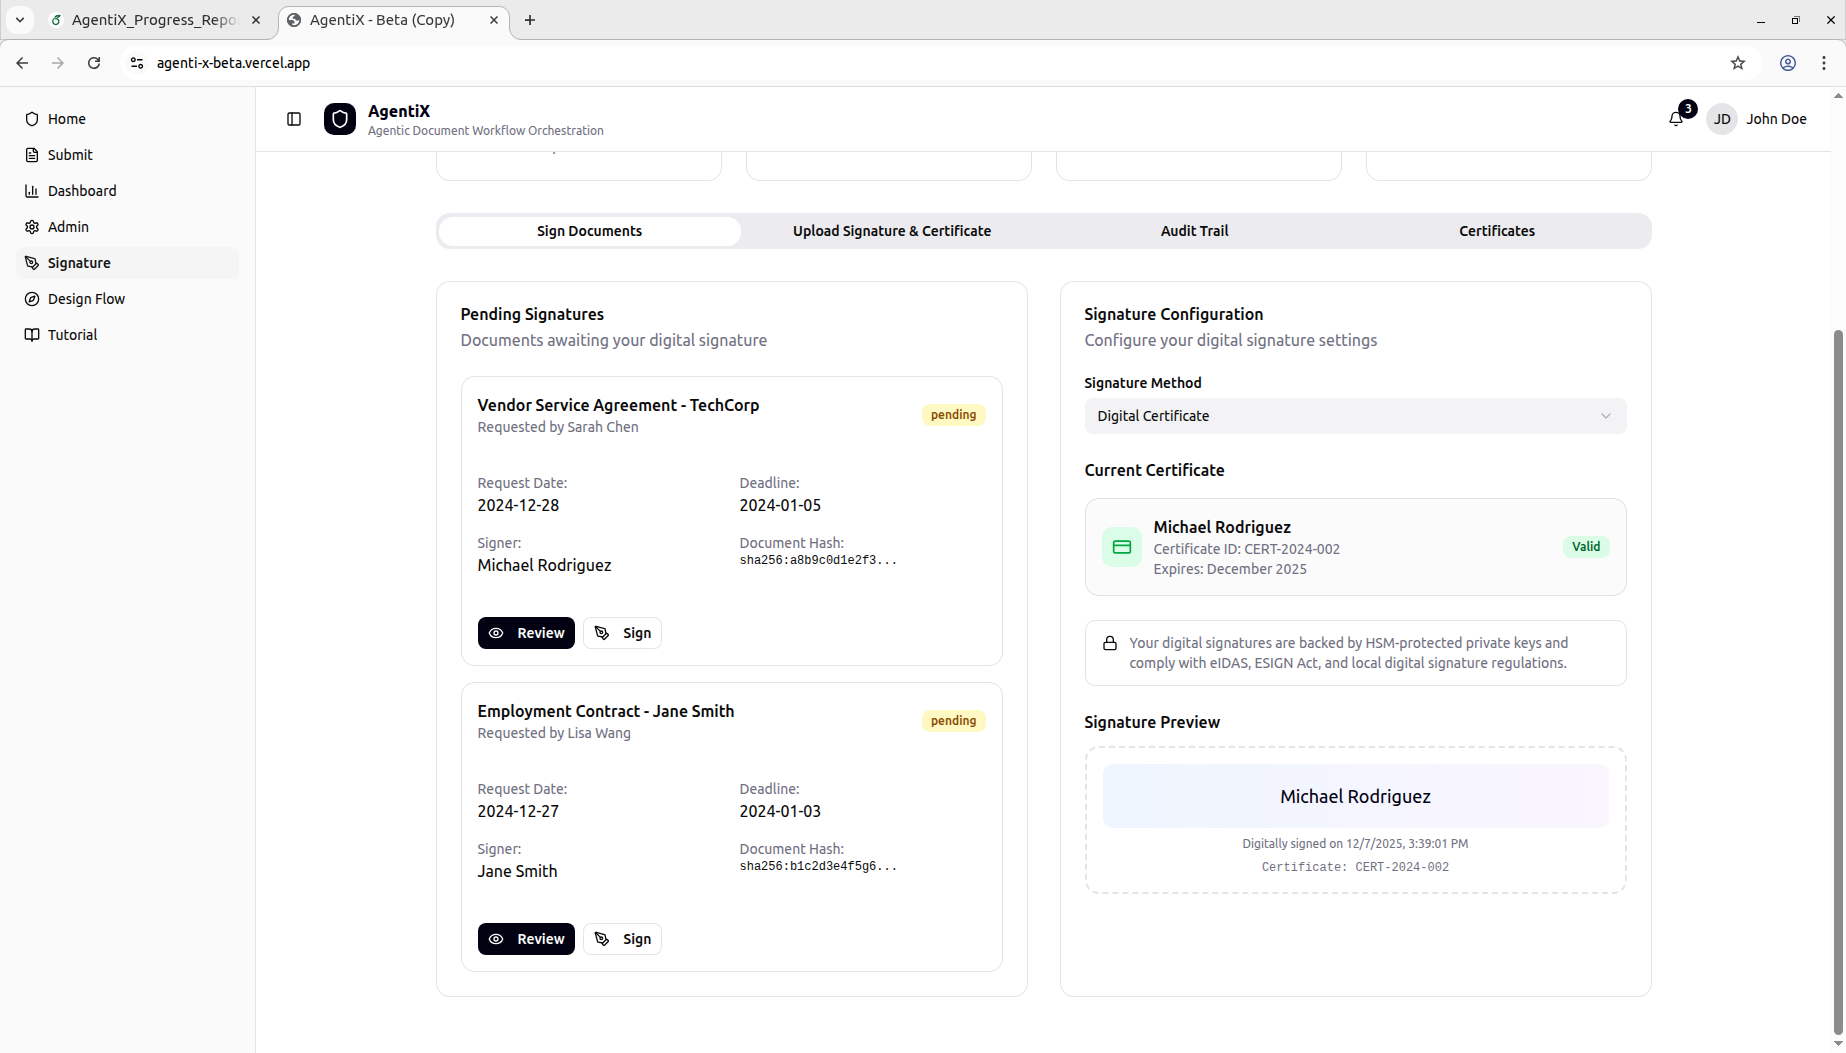
\includegraphics[width=0.9\linewidth]{image/signature_module_placeholder.png}
    \caption{Signature capture dialog: upload interface with drag-and-drop zone prompting ``Click to upload'' (PNG, JPG, PDF, up to 10 MB), and initial capture state ready for signature image submission.}
    \label{fig:signature_capture}
\end{figure}

The Signature Capture interface (Figure~\ref{fig:signature_capture}) provides an intuitive, mobile-friendly method for users to supply their handwritten signature. The capture process supports multiple input modalities:

\begin{itemize}
\item \textbf{Headline and Purpose:} A clear modal title ``Crop your signature'' with supporting text: ``Upload a photo of your signature on white paper, or a PDF of a signed document. Drag the rectangle to move it; drag any handle to resize.'' This immediately communicates the expected input format and user control model.

\item \textbf{Upload Zone:} A large, dashed-border drop zone displays a document icon and text: ``Click to upload'' with supported formats listed (PNG, JPG, PDF) and file-size limit (up to 10 MB). The drag-and-drop affordance encourages visual users to supply signature images without navigating the file system.

\item \textbf{Primary Action Button:} A ``Use this crop'' button (styled in prominent purple) is initially disabled until a valid signature image is uploaded. Once an image is available, the button enables, allowing users to proceed to the cropping/verification step.

\item \textbf{Modal Close:} An ``X'' button in the top-right corner allows users to dismiss the modal without submitting a signature, supporting a low-friction exit path.
\end{itemize}

\subsubsection{Signature Cropping and Processing}
\begin{figure}[htbp]
    \centering
    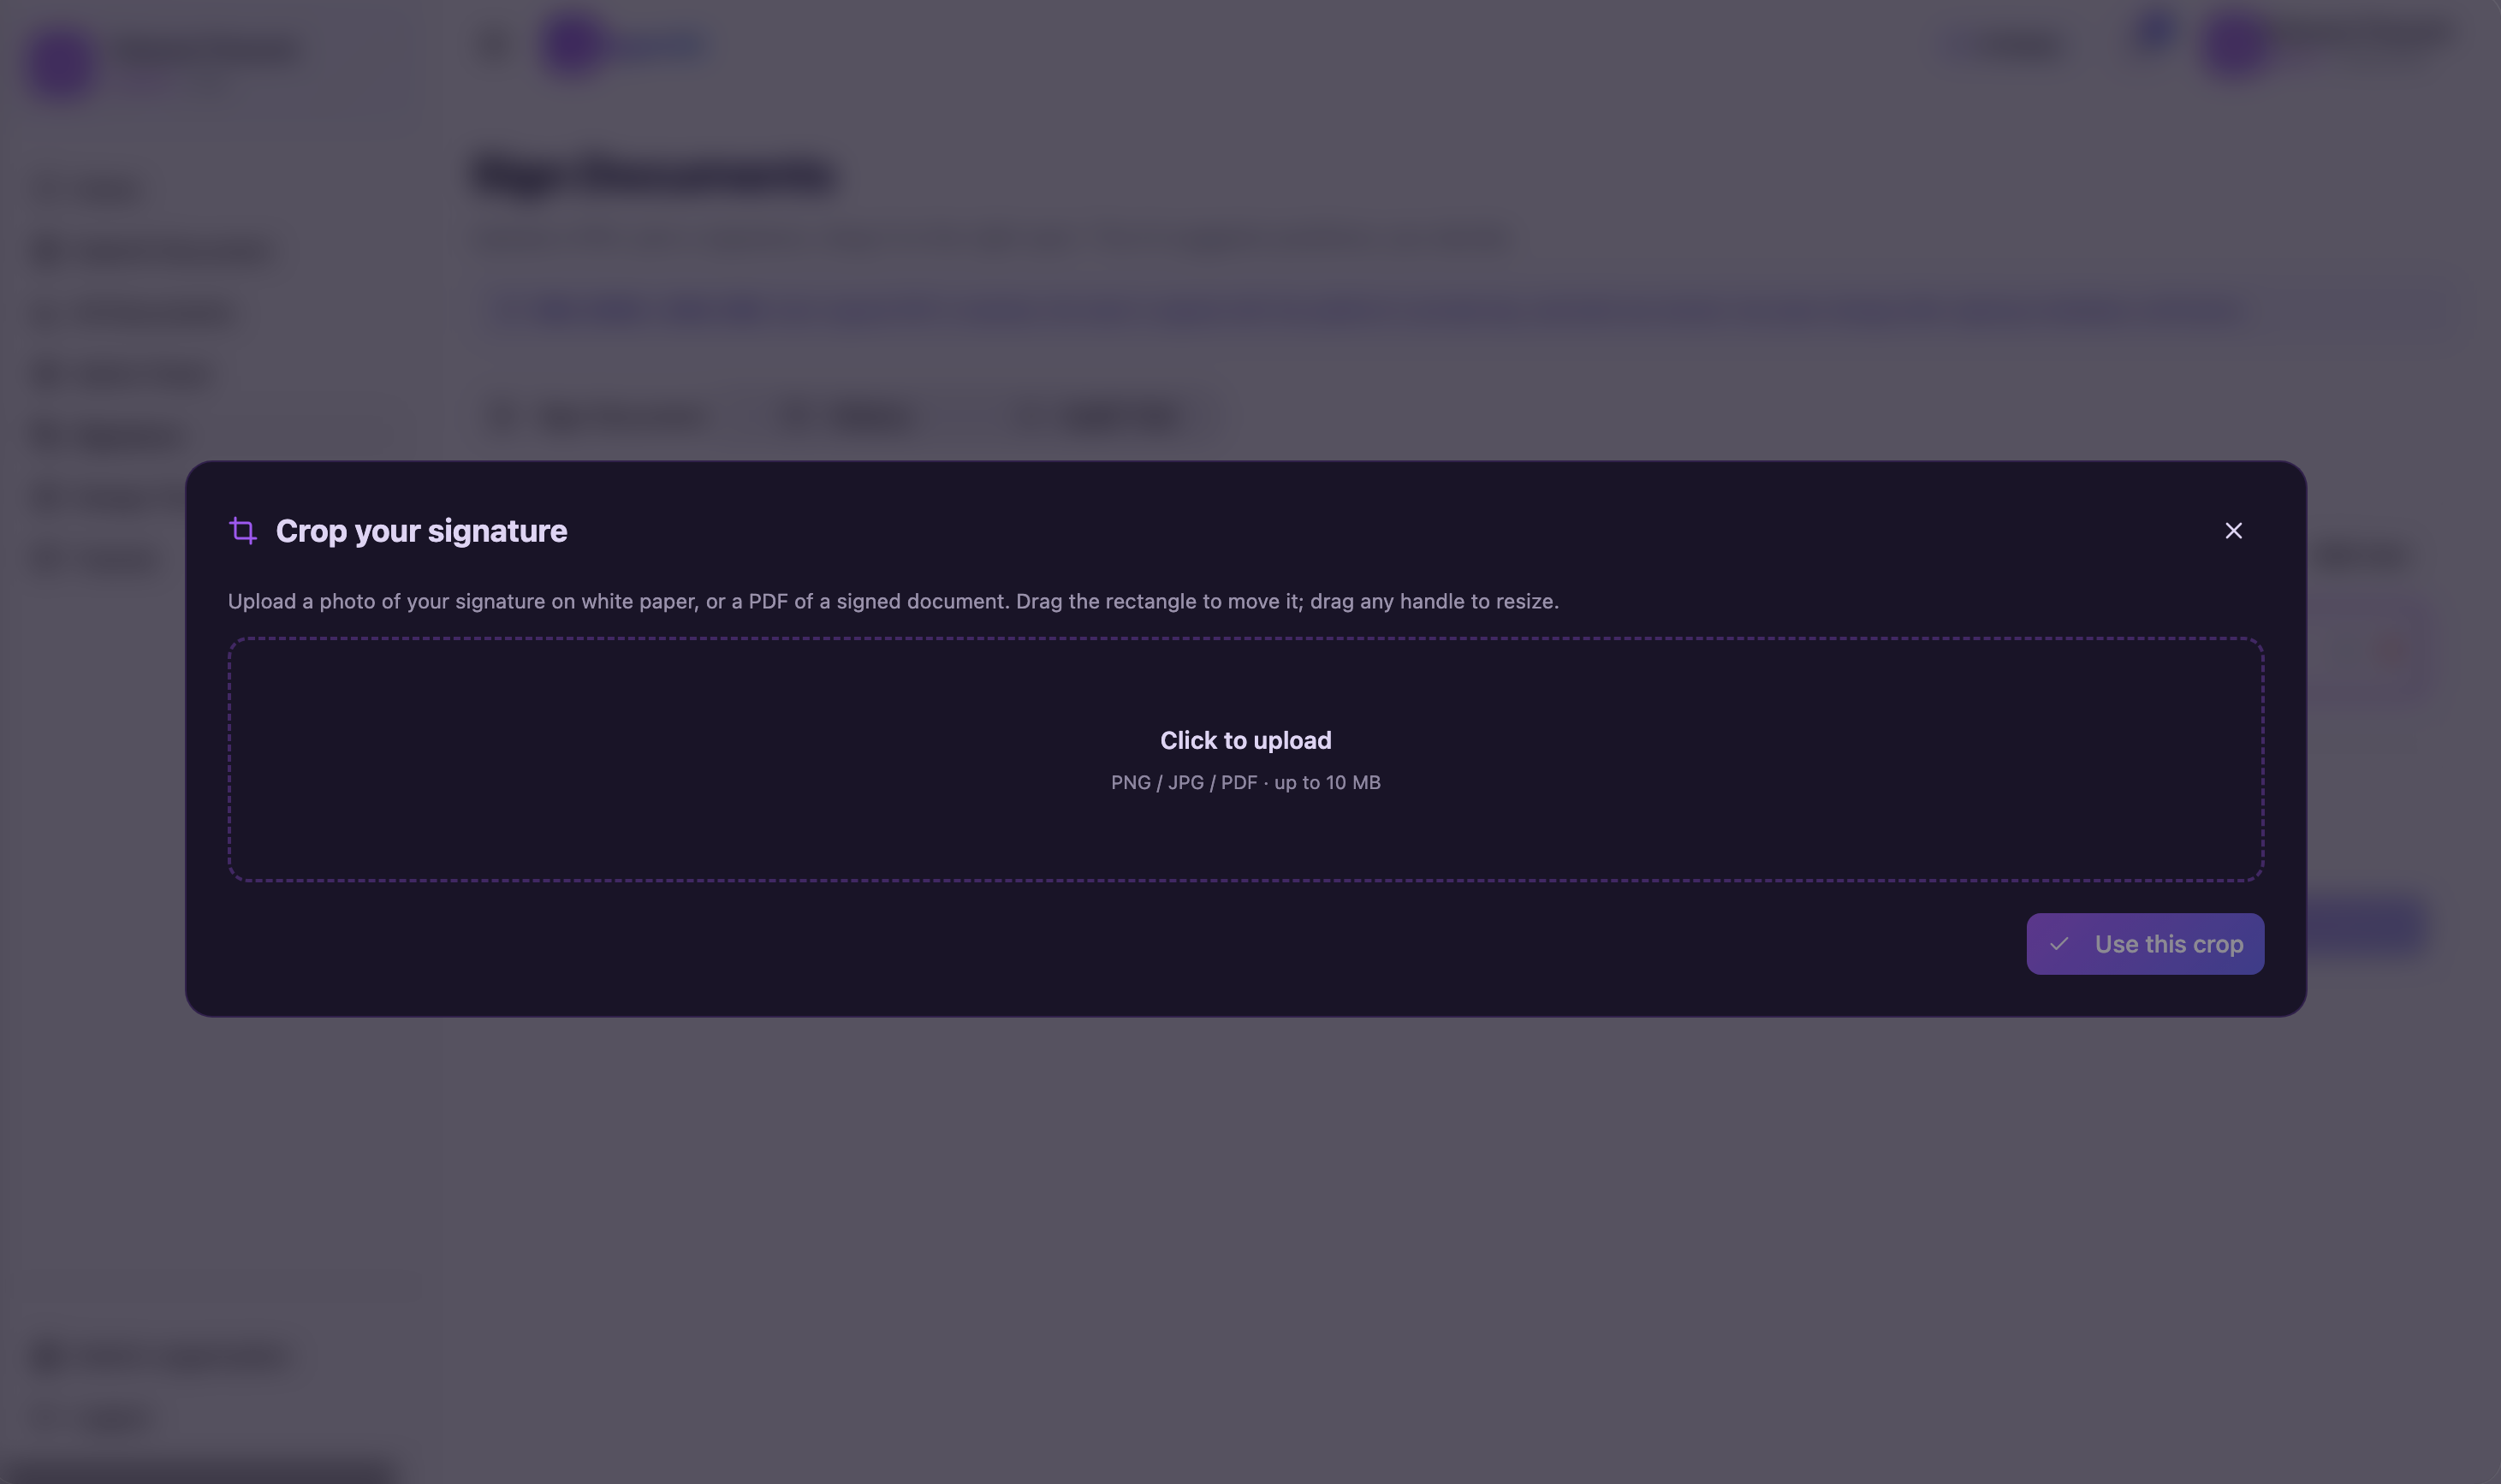
\includegraphics[width=0.9\linewidth]{image/signature_module_placeholder_2.png}
    \caption{Signature cropping interface: uploaded signature image with interactive crop box (resize handles), zoom slider (0-100\%), ``Reset'' button, preview area showing cropped signature (``Apichat Ruangsuk''), checkbox for ``Remove white background (transparent PNG)'', and action buttons (``Pick different file'' / ``Use this crop'').}
    \label{fig:signature_cropping}
\end{figure}

The Signature Cropping interface (Figure~\ref{fig:signature_cropping}) provides precise control over the signature region extracted from the uploaded image. This step ensures that only the actual signature is retained, removing extraneous background:

\begin{itemize}
\item \textbf{Interactive Crop Region:} A resizable rectangular crop box is overlaid on the uploaded image. Visible corner and edge handles allow users to drag and resize the region. Visual feedback (purple dashed outline) indicates the active crop area.

\item \textbf{Zoom Control:} A zoom slider (0--100\%) enables users to magnify or reduce the image for precise positioning. A ``Reset'' button restores the original zoom level and crop box position, supporting easy correction if the user makes undesired adjustments.

\item \textbf{Live Preview:} As users adjust the crop box, a live preview appears in the right panel, showing the extracted signature (e.g., text reading ``Apichat Ruangsuk''). This real-time feedback prevents surprises when finalizing the crop.

\item \textbf{Background Removal Option:} A checkbox labeled ``Remove white background (transparent PNG)'' enables automated background removal, converting white pixels to transparency. This is useful for signatures captured on plain paper, allowing seamless embedding onto documents with varied background colours.

\item \textbf{Action Buttons:} Two buttons at the bottom right:
  - ``Pick different file'': Allows users to discard the current image and upload a new one without restarting the modal.
  - ``Use this crop'' (purple, prominent): Submits the cropped signature for storage and subsequent use in document signing.
\end{itemize}

\subsubsection{Document Signing Workflow}
\begin{figure}[htbp]
    \centering
    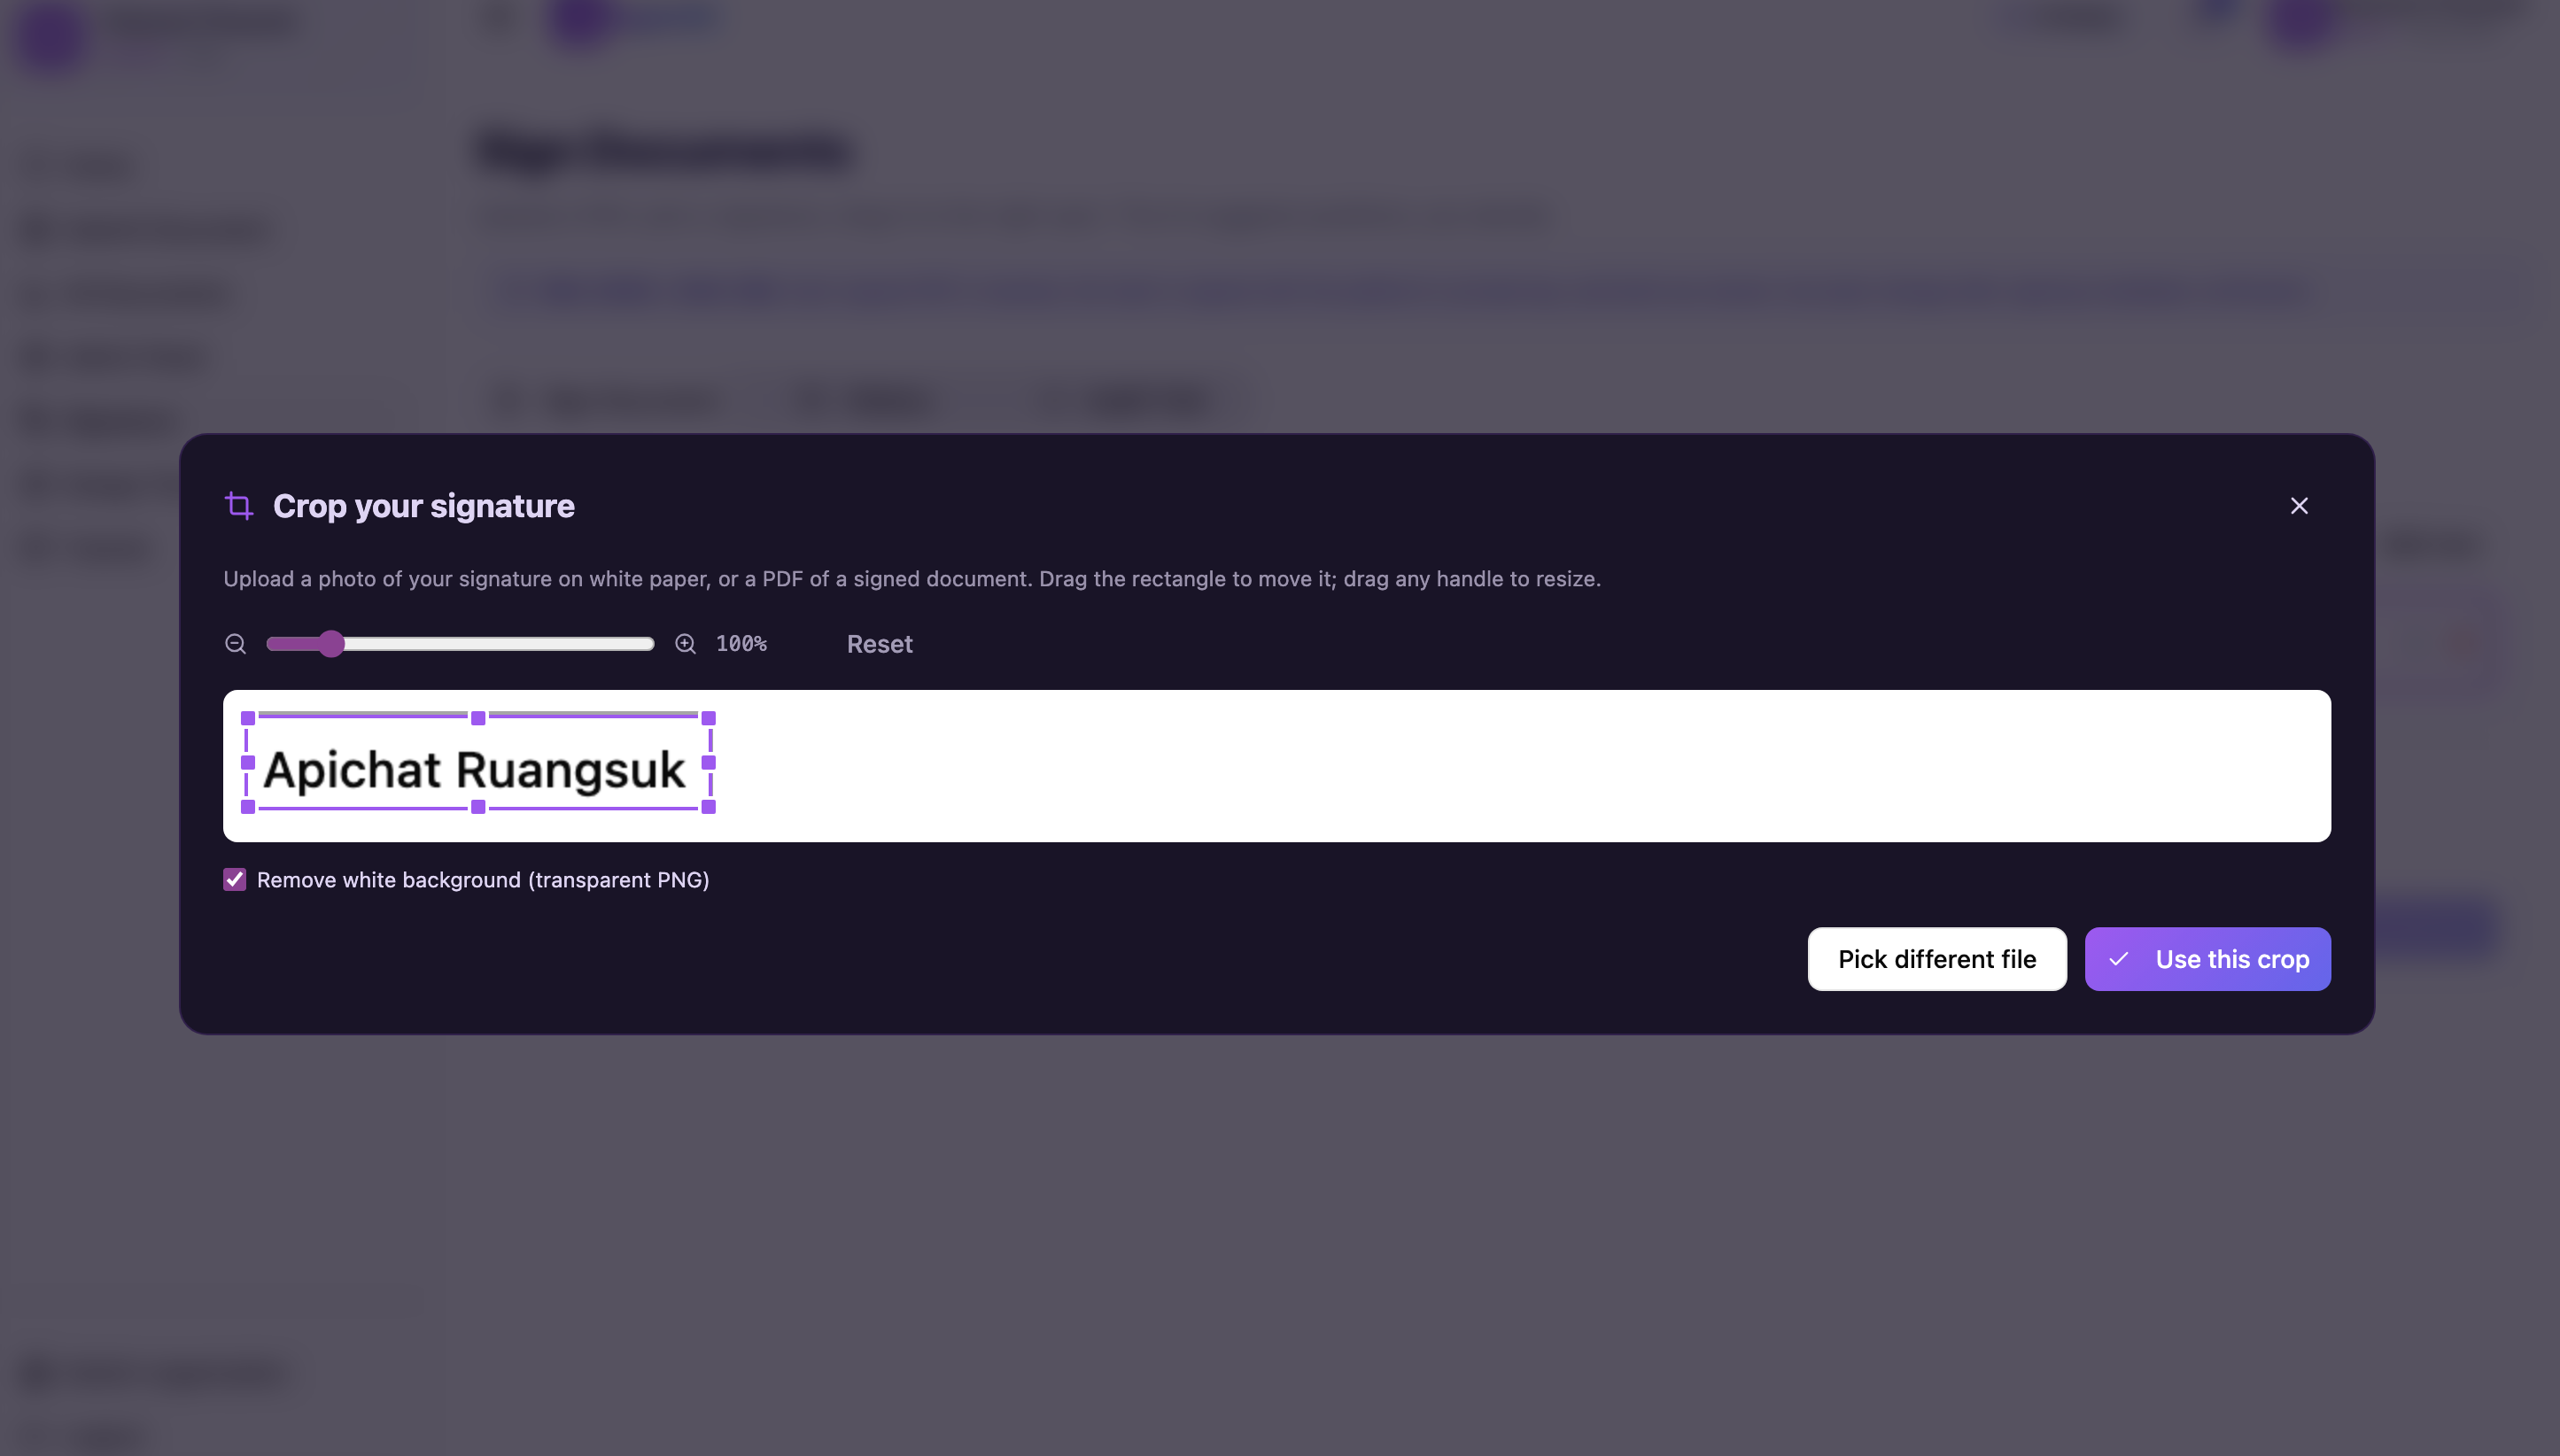
\includegraphics[width=0.9\linewidth]{image/signature_module_placeholder_3.png}
    \caption{Sign Documents interface: two-column layout with left panel showing ``1. Upload PDF'' (drag-and-drop zone for PDFs up to 25 MB), and right panel showing ``2. Pick a signature'' (signature card displaying ``Pakawat Phasook''), ``4. Sign + download'' with a ``Sign + embed'' button. Includes security note about RSA-2048 + SHA-256 encryption.}
    \label{fig:document_signing}
\end{figure}

The Document Signing workflow (Figure~\ref{fig:document_signing}) orchestrates the end-to-end process of applying a digital signature to an approved document. The interface guides users through a clear, step-by-step progression:

\begin{itemize}
\item \textbf{Page Title and Value Proposition:} ``Sign Documents'' with supporting text: ``Upload a PDF, pick a signature, drag it to the right spot. The AI suggests positions; you decide.'' This immediately conveys the workflow's purpose and human-in-the-loop nature.

\item \textbf{Security Information Banner:} A blue info box states: ``RSA-2048 + SHA-256. Each signed PDF is hashed, the hash is signed with the platform's private key, and both are stored. Any byte change after signing invalidates verification.'' This transparent communication reassures users and administrators about cryptographic strength and tamper-detection capability.

\item \textbf{Tabbed Navigation:} Three tabs organize the workflow: ``Sign Document'' (default, active state), ``History'' (previous signatures), and ``Audit Trail'' (immutable log). Users can switch between views without losing progress.

\item \textbf{Step 1: Upload PDF:} A left-side card titled ``1. Upload PDF'' displays a dashed-border drop zone with a document icon and text ``Click to upload PDF'' with file-size limit (up to 25 MB). Clicking or dragging a PDF into this zone initiates the upload.

\item \textbf{Step 2: Pick a Signature:} A right-side card titled ``2. Pick a signature'' displays available signatures. A signature card shows the signer's name (``Pakawat Phasook'') and a visual signature preview. An ``+ Add new'' button allows users to register additional signatures if the desired one is unavailable.

\item \textbf{Step 4: Sign + Download:} Below the signature picker, a card titled ``4. Sign + download'' contains the action button ``Sign + embed'' (purple, prominent). A placeholder note states ``Upload a PDF first,'' indicating that the button is disabled until a valid PDF is uploaded. Once both a PDF and signature are selected, the button enables.

\item \textbf{User-Directed Placement:} The workflow note mentions ``drag it to the right spot,'' implying that after a PDF is uploaded, users can interact with a canvas to position the signature on the document page. AI-assisted suggestions help speed placement, but final placement authority rests with the user.

\item \textbf{Output Artifact:} Clicking ``Sign + embed'' triggers the signing operation: the document is hashed (SHA-256), the hash is digitally signed (RSA-2048 with the platform's private key), and the signature is embedded into the PDF. The resulting signed PDF is offered for download, and a copy is archived for audit and verification.
\end{itemize}

\subsubsection{Signature Management and History}

The Signature Module includes supplementary features that provide long-term manageability and auditability:

\begin{itemize}
\item \textbf{Signature Registry:} Users can store multiple signatures (e.g., formal signature, initials, alternative script) and label them for easy identification. The module presents a list of available signatures during document signing, allowing selection based on context (e.g., formal approval vs. acknowledgment).

\item \textbf{History Tab:} A chronological record of all signatures applied by the user, including document names, timestamps, and verification status. Users can export or re-download previously signed documents without re-signing.

\item \textbf{Audit Trail Tab:} An immutable, cryptographically chained log of all signing events, including: signer identity, document hash, signature hash, timestamp (from trusted time-stamping authority), and verification results. This audit trail satisfies regulatory requirements (e.g., eIDAS, GDPR) and supports forensic investigations if tampering is suspected.

\item \textbf{Verification Service:} AgentiX exposes a public verification endpoint that accepts a signed PDF and returns: signature validity (tamper-free or compromised), signer identity, signing timestamp, and certificate chain status. External parties can verify document authenticity without requiring internal credentials, supporting B2B workflows and legal defensibility.
\end{itemize}

The Signature Module thus transforms document approval from a procedural step into a legally defensible, auditable artifact. Combined with the organizational workflow engine and compliance policies, it ensures that AgentiX-processed documents are indisputable records of organizational decision-making.

\vspace{1em}

\subsection{Conclusion}

The AgentiX web application design successfully integrates complex backend logic (AI routing, Cryptography) with a clean, accessible frontend. The use of a modular architecture ensures that distinct user personas—from general employees submitting requests to administrators managing compliance—have dedicated, optimized workspaces. The design prioritizes transparency, trust, and observability, essential qualities for an enterprise automation platform.

\newpage

\section{Detailed Architecture Implementation}

This section expands upon the architectural overview presented in section 4.2, providing implementation-level details on the backend services, data layer, message queue infrastructure, and monitoring systems that power AgentiX. These implementation details are derived from the production codebase and reflect actual design decisions, patterns, and technologies deployed.

\vspace{1em}

\subsection{Backend API Architecture}

\subsubsection{Serverless and Express-Compatible Design}

The AgentiX backend employs a hybrid deployment strategy that supports both serverless execution (Vercel Functions, AWS Lambda) and traditional Node.js servers (Express on Render). This flexibility is achieved through an adapter pattern that bridges Vercel's request/response model with standard Express middleware.

The API is structured into 11 major feature domains, each containing 2-5 specialized endpoints organized by concern:

\begin{itemize}
    \item \textbf{Documents Management}: Create, retrieve, analyze, sign, and verify documents with automatic versioning and tamper detection
    \item \textbf{Workflow Management}: Fetch pending approvals, submit approval/rejection decisions with optional comments
    \item \textbf{Digital Signatures}: Manage cryptographic signatures, download signed documents, detect tampering
    \item \textbf{AI Services}: Document classification, OCR, chat-based document submission, and AI model fallback
    \item \textbf{Authentication}: Login with email/password or OAuth, handle Google/organization SSO callbacks
    \item \textbf{Organizations}: Create organizations, manage members, parse and confirm organization charts
    \item \textbf{Administration}: User management, department configuration, system seeding for demo/testing
\end{itemize}

\subsection{Service Layer Architecture}

The implementation follows a service-oriented architecture with clear separation of concerns:

\begin{itemize}
    \item \textbf{DocumentService}: Upload, version, retrieve, analyze documents using Repository Pattern
    \item \textbf{WorkflowService}: Execute approval workflows, manage approvals using State Machine pattern
    \item \textbf{SignatureService}: RSA-2048 signing, SHA-256 hashing, signature verification using Cryptographic pattern
    \item \textbf{AIService}: Provider abstraction for Gemini and Typhoon using Factory Pattern
    \item \textbf{AuthService}: JWT validation, password hashing, session management using Token-based authentication
\end{itemize}

\subsubsection{Document Service Implementation}

The DocumentService manages the complete document lifecycle:

\begin{enumerate}
    \item \textbf{Upload Pipeline}: Receives file buffer, computes SHA-256 content hash, uploads to Supabase Storage with versioning
    \item \textbf{Version Control}: Maintains immutable document versions in the database, enabling rollback and audit trails
    \item \textbf{Analysis Pipeline}: Downloads PDF, triggers AI analysis with configured provider (Gemini or Typhoon), automatically creates workflow
    \item \textbf{Status Tracking}: Propagates document state changes (draft → in\_review → approved → signed) through the workflow system
\end{enumerate}

\subsubsection{Workflow Service Implementation}

The WorkflowService orchestrates multi-step approval processes:

\begin{itemize}
    \item \textbf{AI-Driven Generation}: Converts AI classification suggestions into executable workflows with configurable steps
    \item \textbf{Return Loop Logic}: Implements intelligent rejection handling via the return\_on\_reject\_to field, routing documents back to specified previous steps
    \item \textbf{Parallel Approval Support}: Enables team-based approvals by assigning workflow steps to roles rather than individual users
    \item \textbf{Comment Tracking}: Records approver comments and timestamps for complete decision audit trails
\end{itemize}

\subsubsection{AI Service Implementation}

The AIService provides a pluggable architecture for document classification with automatic provider fallback:

\begin{itemize}
    \item \textbf{Provider Abstraction}: Unified interface supporting Google Gemini and SCB10X Typhoon
    \item \textbf{Auto-Fallback Mechanism}: If the primary provider fails, automatically retries with secondary provider
    \item \textbf{Configuration Strategy}: Environment variable AI\_PROVIDER supports ``typhoon'', ``gemini'', or ``auto'' modes
    \item \textbf{Model Selection}: Configurable model names and parameters per provider with temperature and token controls
\end{itemize}

The Gemini Client directly processes PDFs as base64 for document analysis, leveraging Gemini's vision capabilities. The Typhoon Client focuses on Thai language processing, requiring OCR preprocessing before analysis.

\vspace{1em}

\subsection{Data Layer Architecture}

\subsubsection{Database Schema Design}

The data layer is implemented using Supabase (PostgreSQL-backed) with a carefully designed schema supporting document versioning, audit trails, and role-based access control.

\subsubsection{Core Data Models}

Key tables include: users (identity and roles), documents (metadata and status), document\_versions (immutable version history), workflows (approval definitions), workflow\_steps (individual approval nodes), approvals (decision records), ai\_classifications (analysis results), signatures (digital signature records), and audit\_logs (complete activity logs).

\subsubsection{Critical Design Patterns}

%% Help me check
\begin{itemize}
    \item \textbf{Immutable Versioning}: Document versions are write-once; updates create new versions rather than modifying existing ones, ensuring audit compliance
    \item \textbf{Cascading Foreign Keys}: Document deletion automatically removes related versions, workflows, and signatures, maintaining referential integrity
    \item \textbf{JSONB Storage}: Complex structures stored as JSONB for flexible schema evolution
    \item \textbf{Unique Constraints}: Composite unique constraints prevent duplicate records
\end{itemize}

\subsubsection{Performance Optimization}

Strategic indexes optimize common query patterns, including the following:

%% Help me check
\begin{itemize}
  \item \texttt{idx\_documents\_owner} for user document retrieval.
  \item \texttt{idx\_documents\_status} for status filtering.
  \item \texttt{idx\_workflow\_steps\_status} for finding pending approvals.
  \item \texttt{idx\_approvals\_step} for step approval lookup.
  \item \texttt{idx\_signatures\_version} for locating signatures for each document version.
\end{itemize}

\subsubsection{Row-Level Security}

PostgreSQL Row-Level Security policies enforce access control: Users table restricted to admins and self-owner, Documents table accessible to owner/workflow participants/admin, Workflows table mirrors document visibility, Approvals table restricted to step approver or admin.

\subsubsection{Document Storage Strategy}

Documents stored in Supabase Cloud Storage with path hierarchy: documents/\{docId\}/v\{version\_no\}.pdf. Backend uploads use service-role API key. Frontend downloads use time-limited signed URLs (1-hour expiry). Lifecycle policies auto-delete files when records removed. SHA-256 hash stored in database for tamper detection.

\vspace{1em}

\subsection{Message Queue and Event System}

The current implementation uses synchronous API handlers with database-driven event tracking. The architecture supports future async patterns through structured event logs.

\subsection{Event-Driven Patterns}

\subsubsection{Document Analysis Workflow}

Document analysis is triggered via POST /documents/\{id\}/analyze, which downloads the PDF, calls the AI service, stores classification results, creates workflow steps, and transitions document to ``in\_review''.

\subsubsection{Approval Decision Workflow}

Approvals triggered via POST /workflows/\{stepId\}/action record the decision, update status, route rejections if specified, and advance or loop the document.

\subsection{Future Event-Driven Architecture}

The schema includes email\_notifications table for future message broker integration. Recommended events: ai.analysis.started (AI Worker), approval.requested (Notification Service), document.signed (Audit Logger), workflow.completed (Email/SMS Notifier).

\vspace{1em}

%% Help me check
\section{Monitoring and Observability}

\subsection{Health Check Endpoint}

Platform implements GET /api/v1/healthz endpoint returning system status with timestamp for continuous availability monitoring.

\subsection{Audit Logging}

Audit\_logs table records every significant action: Timestamp, User, Action Type, Entity Type, Entity ID, Result. Immutable logs retained for compliance (7 years for financial documents). Admin console allows filtering by user, action type, or date range.

\subsection{Error Handling and Logging}

Consistent error handling: 400 Bad Request for validation, 401 Unauthorized for auth failures, 403 Forbidden for authorization, 404 Not Found for missing resources, 500 Server Error with correlation ID for tracing.

% Deployment and DevOps details integrated into Chapter 4
\section{Deployment and DevOps}

This chapter details the deployment architecture, CI/CD pipelines, infrastructure configuration, and operational procedures for the AgentiX platform. The deployment strategy supports both managed cloud services and enterprise-private installations.

\vspace{1em}

\subsection{Deployment Architecture}

\subsubsection{Hybrid Deployment Model}

AgentiX supports two primary deployment configurations:

\paragraph{Cloud Deployment (Managed Service)}

\begin{itemize}
    \item \textbf{Frontend}: Deployed on Vercel (Vite SPA)
    \item \textbf{Backend}: Deployed on Render.com (Node.js Express)
    \item \textbf{Database}: Supabase Cloud (PostgreSQL)
    \item \textbf{Storage}: Supabase Cloud Storage (AWS S3 backed)
    \item \textbf{Region}: Singapore region optimized for Southeast Asia latency
    \item \textbf{Target}: Organizations seeking managed infrastructure with minimal DevOps overhead
\end{itemize}

\subsubsection{Enterprise-Private Deployment}

\begin{itemize}
    \item \textbf{Frontend}: Self-hosted on Kubernetes or traditional servers
    \item \textbf{Backend}: Self-hosted Node.js on VMs or Kubernetes
    \item \textbf{Database}: PostgreSQL on enterprise infrastructure
    \item \textbf{Storage}: MinIO, AWS S3, or local filesystem
    \item \textbf{Network}: Private VPN or air-gapped deployment
    \item \textbf{Target}: Organizations with strict data residency requirements
\end{itemize}

\subsubsection{Cloud Deployment Configuration}

\paragraph{Vercel Frontend Deployment}

\begin{itemize}
\item Build configuration: \texttt{npm run build} produces the \texttt{dist/} folder via Vite.
\item SPA rewrite: Non-matching routes redirect to \texttt{/index.html}.
\item Environment variables: \texttt{VITE\_SUPABASE\_URL}, \texttt{VITE\_SUPABASE\_ANON\_KEY}, and \texttt{VITE\_API\_URL}.
\item Asset delivery: Files are served globally through Vercel's CDN.
\item Preview deployments: Automatic preview deployments are generated for pull requests.
\end{itemize}

\paragraph{Render Backend Deployment}

%% Help me check
\begin{itemize}
    \item \textbf{Runtime}: Node.js
    \item \textbf{Region}: Singapore
    \item \textbf{Build}: npm install \&\& npx tsc -p tsconfig.server.json
    \item \textbf{Start}: node dist-server/server/index.js
    \item \textbf{Health Check}: GET /api/v1/healthz (polled every 30 seconds)
\end{itemize}

\begin{itemize}
\item Render dashboard environment variables include: \texttt{SUPABASE\_URL}, \texttt{SUPABASE\_SERVICE\_ROLE\_KEY}, \texttt{GEMINI\_API\_KEY}, and \texttt{TYPHOON\_API\_KEY}.
\item Additional variables include: \texttt{AI\_PROVIDER}, \texttt{PORT}, and \texttt{FRONTEND\_URL}.
\end{itemize}

\subsubsection{Enterprise-Private Deployment}

% Help me check
For organizations requiring on-premise or private cloud deployments, AgentiX provides container-based deployment: Frontend container with Nginx for Vite SPA serving, Backend container with Node.js runtime, PostgreSQL database in customer infrastructure, optional Kubernetes support with Helm charts, configurable storage backends (MinIO, S3, local filesystem).

\vspace{1em}

%% help me check
\subsection{Environment Configuration}

\subsubsection{Frontend Configuration}

\begin{itemize}
\item \texttt{VITE\_SUPABASE\_URL}: Points to the Supabase project URL.
\item \texttt{VITE\_SUPABASE\_ANON\_KEY}: Provides the public authentication key.
\item \texttt{VITE\_API\_URL}: Sets the backend API base URL.
\end{itemize}

\subsubsection{Backend Configuration}

\begin{itemize}
\item \texttt{SUPABASE\_URL}: Points to the same Supabase project as the frontend.
\item \texttt{SUPABASE\_SERVICE\_ROLE\_KEY}: Provides private administrative access.
\item \texttt{DATABASE\_URL}: Contains the PostgreSQL connection string.
\item \texttt{AI\_PROVIDER}: Selects the provider (``typhoon'', ``gemini'', or ``auto'').
\item \texttt{GEMINI\_API\_KEY}: Provides Gemini access.
\item \texttt{TYPHOON\_API\_KEY}: Provides Typhoon access.
\item \texttt{AGENTIX\_PRIVATE\_KEY\_PEM}: Contains the RSA-2048 private key for signing.
\item \texttt{PORT}: Specifies the listening port (default 8080).
\item \texttt{FRONTEND\_URL}: Specifies the frontend origin for CORS.
\end{itemize}

\subsubsection{Secrets Management}

Cloud deployments use Vercel/Render dashboard secrets. Local development uses .env.local file (excluded from version control). Enterprise deployments integrate with corporate key management systems (e.g., HashiCorp Vault). Key rotation scheduled for API keys, database passwords, and signing keys.

\vspace{1em}

\subsection{Build and Deployment Pipelines}

\subsubsection{Build Process}

\paragraph{Frontend Build}

npm run build produces TypeScript compilation (src/ → dist/), React component bundling via Vite, CSS/Tailwind processing, asset optimization (images, fonts), and source map generation for error tracking. Target: ES2020 JavaScript with tree-shaking. Output size approximately 200-300 KB gzipped.

\paragraph{Backend Build}

npm run build:server compiles TypeScript (server/, api/, lib/ → dist-server/), bundles dependencies, producing executable dist-server/server/index.js ready for Node.js execution. Target: CommonJS for Node.js 18+.

\subsubsection{CI/CD Pipelines}

\paragraph{GitHub Actions CI Pipeline}

Triggered on push to main and pull requests: Checkout code, setup Node.js v20, install dependencies (npm ci), build frontend, build backend, status blocks merge if build fails.

\paragraph{Production Deployment}

Trigger: Push to main branch after pull request merge. Frontend deployed to Vercel CDN (typically 2-3 minutes). Backend restarted on Render (typically 5-7 minutes). Database schema changes require manual migrations. Git revert reverts to previous state.

\vspace{1em}

\subsection{Containerization}

\subsubsection{Backend Container}

Multi-stage build: FROM node:20-alpine, copy package files, npm ci --only=production, copy built dist-server/, expose port 8080, start with node dist-server/server/index.js. Image size approximately 150 MB uncompressed (50 MB compressed). Non-root user recommended for production.

\subsubsection{Frontend Container}

Multi-stage build: Builder stage compiles Vite SPA, nginx stage serves static files. FROM nginx:alpine in final stage. Size approximately 25 MB. Health check at / for liveness probe.

\subsubsection{Container Registry}

Cloud deployments use platform registries (Vercel, Render). Enterprise deployments push to Docker Hub, AWS ECR, or private registry. Tagging: version tags (v1.0.0), environment tags (staging, prod), commit SHAs. Automated vulnerability scanning on push.

\vspace{1em}

\subsection{Infrastructure as Code}

\subsubsection{Vercel Configuration}

vercel.json defines buildCommand, outputDirectory, framework, and SPA routing rewrite rules.

\subsubsection{Render Configuration}

render.yaml specifies service type (web), runtime (node), region (singapore), build command, start command, health check path, and environment variables.

\subsubsection{Kubernetes Deployment}

Helm charts provide declarative infrastructure for organizations deploying on Kubernetes, supporting configuration of image registries, resource limits, autoscaling, service discovery, and storage.

\vspace{1em}

\subsection{Operational Procedures}

\subsubsection{Service Monitoring}

Health checks: Platform providers monitor endpoints automatically. Log aggregation: Errors logged to stderr; aggregated by providers. Metrics: Response times, error rates, CPU/memory tracked. Alerting: Email notifications on service degradation.

\subsubsection{Database Backups}

Automated daily backups (cloud); enterprise uses pg\_dump. 7-day retention (cloud). Point-in-time restore (cloud). RPO target: 1 hour maximum data loss. RTO target: 4-hour service restore.

\subsubsection{Scaling Strategy}

Frontend: Vercel auto-scales CDN. Backend: Render vertical scaling; Kubernetes horizontal scaling. Database: Read replicas with connection pooling. Storage: Unlimited files, no scaling needed.

% Security and cryptography details integrated into Chapter 4
\section{Security and Cryptography Implementation}

This chapter provides comprehensive documentation of the security architecture, cryptographic implementation, authentication mechanisms, and compliance controls that protect AgentiX from unauthorized access, data breaches, and document tampering.

\vspace{1em}

\subsection{Cryptographic Implementation}

\subsubsection{Digital Signature Mechanism}

AgentiX implements RSA-2048 digital signatures to provide non-repudiation and tamper detection for approved documents.

\paragraph{RSA-2048 Key Generation}

Key size of 2048-bit RSA provides security equivalent to AES-112 and remains recommended by NIST through 2030. Key pairs generated per organizational user or globally per system. Private keys stored in AGENTIX\_PRIVATE\_KEY\_PEM environment variable (encrypted at rest in key management systems). Annual key rotation recommended; old keys archived for signature verification.

\paragraph{Signing Algorithm}

Algorithm: RSA-PSS (RSA Probabilistic Signature Scheme) with SHA-256 hash function, 32-byte salt length, and PKCS\#1 v2.1 padding. Process: Document content hashed using SHA-256, random 32-byte salt generated, PSS padding applied to hash and salt, RSA private key operation performs signature, signature appended to document.

RSA-PSS advantages: Probabilistic padding provides semantic security (same message produces different signatures), resistance to chosen-ciphertext attacks, FIPS 186-4 approved.

\paragraph{Signature Verification}

Process: Extract signature from document, hash document content (SHA-256), RSA public key operation on signature, extract salt and hash from PSS padding, compare extracted hash with computed hash. Result: Valid or Invalid determination.

\subsubsection{Content Hashing}

SHA-256 hash generation produces 256-bit (32-byte) output displayed as hexadecimal. NIST recommends SHA-256 for document hashing. Use cases include document content integrity verification, change detection for bit-matching validation, and storage in database for tamper detection.

Hash computed and stored in database during document upload. On document retrieval, hash recomputed and compared with stored value. Any single-bit modification produces different hash; tampering detected. Collision probability negligible (less than $2^{-128}$ for $2^{32}$ documents).

\vspace{1em}

\subsection{Encryption at Rest and In Transit}

\subsubsection{Transport Layer Security}

\paragraph{TLS 1.3 Configuration}

\begin{itemize}
\item Protocol version: TLS 1.3 (RFC 8446).
\item Cipher suites: \texttt{TLS\_AES\_256\_GCM\_SHA384} (primary), \texttt{TLS\_AES\_128\_GCM\_SHA256} (fallback), and \texttt{ChaCha20\_Poly1305} for older clients.
\item Certificate renewal: Valid certificates are renewed automatically 30 days before expiry.
\item HSTS: HTTP Strict Transport Security is enforced with \texttt{max-age=63072000}.
\item Certificate pinning: Optional for enterprise deployments to reduce MITM risk.
\end{itemize}

\paragraph{TLS Implementation}

Frontend served via HTTPS by Vercel or Nginx with TLS termination. Backend configured with TLS/SSL certificates; also connects to database via TLS. Intermediate and root CA certificates included for verification. ECDHE key exchange ensures Perfect Forward Secrecy: session compromise doesn't expose past messages.

\subsubsection{Database Encryption}

Supabase encrypts database volumes using AES-256 (managed by AWS/Google). Connection to database enforced via TLS 1.3. Encryption keys managed by cloud provider (users cannot access). Enterprise deployments can enable pgcrypto extension for per-row encryption, integrate with corporate HSM/KMS, use encrypted backups in separate vaults.

\subsubsection{Storage Encryption}

Supabase Storage uses AES-256 server-side encryption on S3 buckets. Enterprise storage configured with AES-256 encryption on MinIO; keys rotated monthly. High-sensitivity documents encrypted with additional application-layer encryption.

\vspace{1em}

\subsection{Authentication and Authorization}

\subsubsection{Authentication Mechanisms}

\paragraph{Password-Based Authentication}

Algorithm: bcrypt with 10 salt rounds. Password requirements: minimum 8 characters, at least one uppercase, lowercase, number, and special character, no dictionary words. Process: User enters password, random salt generated (bcrypt embedded), password hashed $2^{10}$ times, hash stored (not password). Verification: Password compared during login using bcrypt compare.

\paragraph{Multi-Factor Authentication}

Recommended for administrative users: Time-Based OTP (Google Authenticator, Authy compatible), SMS OTP (six-digit codes), backup codes generated during setup, recovery mechanisms if MFA unavailable.

\paragraph{OAuth and SSO Integration}

Google OAuth 2.0 login with Google account (leverages Google's MFA). Organization SSO with SAML 2.0 integration for corporate identity providers (Active Directory, Okta, Azure AD). Just-In-Time provisioning creates accounts on first SSO login. Attribute mapping from SSO provider maps department, role, email to AgentiX attributes.

\subsubsection{Authorization Models}

\paragraph{Role-Based Access Control}

Five primary roles: Employee (submit documents, view personal history), Manager (employee permissions + approve subordinates), Department Head (manager permissions + policy configuration), C-Level (department head permissions + org settings), Admin (all permissions + user management + audit logs).

\paragraph{Session Management}

Token type: JWT issued by authentication endpoint. Token lifetime: 24 hours (refresh token 7 days). Storage: Browser localStorage (frontend) or HTTP-only cookies. Validation: Backend verifies JWT signature and expiration on every API request. Logout invalidates token (removed from whitelist or blacklisted).

\vspace{1em}

\subsection{Data Protection and Privacy}

\subsubsection{PDPA Compliance}

AgentiX implements controls for Thailand's Personal Data Protection Act: Collect only necessary data explicitly requested; obtain explicit consent before processing (records retained); store only required fields; implement user rights (access, correct, deletion); notify breach to individuals within 72 hours per PDPA requirements.

\subsubsection{Sensitive Data Handling}

Documents marked as Confidential, Internal, or Public. All document accesses recorded with timestamp and user ID. Sensitive fields (SSN, bank account) masked in logs and reports. Deleted documents securely wiped (cryptographic erasure).

\subsubsection{ISO 27001 Controls}

Implemented controls include: Security policies documented and communicated, CISO and security team roles defined, documented access provisioning, endpoint protection requirements for BYOD, RBAC with least privilege, RSA-2048/SHA-256/TLS 1.3 cryptography, audit logging for sensitive operations, network isolation via Supabase, documented security requirements in specifications.

\vspace{1em}

\subsection{Threat Mitigation}

\subsubsection{Common Attack Prevention}

\paragraph{SQL Injection}

Prevention: Parameterized queries via Supabase (no raw SQL), input validation against expected format, database user roles restricted to necessary tables.

\paragraph{Cross-Site Scripting}

React automatically escapes user input; no dangerouslySetInnerHTML used. CSP headers restrict script execution origins. File uploads scanned for embedded scripts.

\paragraph{CSRF}

CSRF tokens generated per session and validated on state-changing operations. Cookies set with SameSite=Strict to prevent cross-site requests. CORS whitelist specific origins; reject unknown origins.

\paragraph{Denial of Service}

API Gateway implements per-user rate limits (e.g., 100 requests/minute). Requests exceeding 50 MB rejected. Long-running operations timeout after 5 minutes. Web Application Firewall blocks patterns associated with DoS attacks.

\subsubsection{Vulnerability Management}

Dependency scanning (npm audit) run on every build. Static analysis tools scan code for security issues. Annual external penetration testing. Security incidents logged, investigated, and remediated.

\vspace{1em}

\subsection{Security Monitoring and Incident Response}

\subsubsection{Security Monitoring}

Audit logs record all sensitive operations with user, timestamp, action, result. Anomalies detected (e.g., failed logins, unusual IP access). Automated alerts on exceeding thresholds. Logs forwarded to SIEM (enterprise).

\subsubsection{Incident Response}

Detection: Security team alerted via email/SMS on suspicious activity. Investigation determines incident impact. Containment: Affected accounts locked/suspended; compromised credentials rotated. Eradication: Root cause determined; vulnerability patched. Recovery: Systems restored from clean backups; monitoring enhanced. Notification: Users notified within 72 hours per PDPA. Post-mortem: Security review conducted; preventive measures implemented.

%% Help me check
\subsection{System Testing}

System testing validates that AgentiX operates correctly as an integrated platform after implementation. The purpose of this phase is to verify that document submission, AI-assisted classification, approval routing, digital signing, audit logging, and notification delivery work together reliably under realistic operating conditions. Testing is performed after unit and integration testing so that end-to-end behavior can be evaluated from the perspective of actual users and administrators.

\subsubsection{Testing Objectives}

The main objectives are to confirm functional correctness, identify defects in cross-module interactions, and evaluate whether the deployed system satisfies performance, security, and usability expectations. The testing process also checks whether the system behaves predictably when invalid input, network interruptions, or workflow exceptions occur.

\subsubsection{Functional Test Scope}

The system test scope covers the major business flows of AgentiX:

\begin{itemize}
  \item \textbf{User authentication and role-based access}: verify login, logout, session validation, password failure handling, and permission boundaries for employees, managers, administrators, and executives. Each role should only access the functions, documents, and dashboards explicitly granted by the authorization model.
  \item \textbf{Document upload, metadata capture, and storage validation}: confirm that supported file types can be uploaded successfully, metadata is recorded correctly, invalid or oversized files are rejected with clear messages, and uploaded documents are stored and retrieved without corruption.
  \item \textbf{AI-based document classification and workflow recommendation}: test whether the system can analyze representative document samples, assign suitable categories, and recommend an approval path that matches business rules. The test should also observe how the system behaves when confidence is low or when document content is incomplete.
  \item \textbf{Approval routing, return-loop handling, and final decision tracking}: verify sequential and parallel approval flows, escalation behavior, rejection handling, reassignment, and the intelligent return loop. Status transitions should remain accurate from initial submission through final approval or rejection.
  \item \textbf{Digital signature generation, verification, and tamper detection}: confirm that the system can generate signatures for approved documents, validate them correctly, and detect file modifications after signing. Testing should also ensure that invalid certificates, altered payloads, or mismatched verification inputs produce explicit failure results.
  \item \textbf{Audit logging, notification delivery, and dashboard status updates}: verify that important actions are written to audit logs with correct timestamps and user references, notifications are sent to the appropriate participants, and dashboard views reflect the latest workflow state without inconsistency.
\end{itemize}

\subsubsection{Test Types}

Several types of testing are used to evaluate the platform comprehensively:

\begin{itemize}
  \item \textbf{Functional testing}: verifies that each complete workflow produces the expected outcome from the user perspective. This includes document submission, AI analysis, approval decisions, return-loop correction, final approval, and signature verification. The goal is to confirm that business rules are implemented correctly and that normal user operations complete without logical errors.
  \item \textbf{Integration testing}: checks communication and data consistency between frontend, backend, database, storage, authentication provider, and AI services. This form of testing is important because AgentiX depends on multiple connected components, and failures often appear at the boundaries between systems rather than inside a single module.
  \item \textbf{Performance testing}: measures response time, throughput, and behavior under concurrent usage. Example concerns include the time required to upload documents, generate workflow recommendations, load dashboards, and complete approval actions when multiple users access the platform at the same time.
  \item \textbf{Security testing}: validates access control, input validation, audit logging, and resistance to common attacks such as unauthorized access, injection attempts, tampered requests, and session misuse. It also checks whether sensitive actions are properly recorded and whether protected resources remain inaccessible to users without the required role.
  \item \textbf{User acceptance testing}: confirms that target users such as employees, approvers, and administrators can complete realistic tasks effectively in an environment that reflects normal usage. This testing helps determine whether the workflow design, terminology, feedback messages, and interface behavior are understandable and practical for real organizational deployment.
\end{itemize}

\subsubsection{Representative Test Scenarios}

Representative scenarios include successful submission and approval of a finance document, rejection and return to the responsible staff member, signature verification after approval, failed login attempts with incorrect credentials, and attempts to access resources without sufficient permissions. Additional scenarios should include malformed uploads, expired sessions, delayed external AI responses, and partial service outages to confirm graceful error handling.

\subsubsection{Acceptance Criteria}

The system is considered ready for deployment when critical workflows complete without blocking defects, security controls operate as designed, and test users can finish key approval tasks within acceptable time. In addition, logs must record important actions correctly, signed documents must pass verification, and failure cases must return clear and recoverable error messages.

\subsubsection{Testing Tools and Environment}

Testing can be performed in a staging environment that mirrors production deployment as closely as possible. Frontend behavior may be tested through browser-based scenarios, backend APIs through automated request scripts, and database correctness through controlled test datasets. Where possible, mock services should be prepared for external AI or notification providers so that failure conditions can be reproduced consistently.

\section{Case Studies and Use Cases}

This chapter presents representative scenarios that show how AgentiX can be applied in real organizations. The examples are intentionally generic so they can be adapted to different business environments.

\subsection{Finance Department Approval Workflow}

A finance team often needs to route budgets, payment requests, and contract renewals through several approvers. In the proposed workflow:

\begin{itemize}
  \item The submitter uploads a payment or budget document.
  \item AgentiX classifies the document as finance-related and identifies the required reviewers.
  \item The workflow is routed to the budget owner, finance manager, and final executive approver if thresholds are exceeded.
  \item If a reviewer rejects the request, the return loop routes the document back to the responsible finance staff member for correction.
\end{itemize}

This use case demonstrates how AgentiX reduces delays caused by email-based approvals and makes financial authorization more traceable.

\subsection{Legal Contract Review Process}

Legal teams typically need to review contract wording, obligations, and risk clauses before signature. AgentiX can support this process by:

\begin{itemize}
  \item Extracting clause-level text from uploaded contracts.
  \item Highlighting legal terms, deadlines, penalties, and unusual obligations.
  \item Routing the document to legal counsel before executive signature.
  \item Preserving the signed document together with an audit trail for compliance review.
\end{itemize}

The system is especially useful when contracts come from many departments and require consistent legal oversight.

\subsection{HR Document Processing}

Human resources teams often manage leave requests, policy acknowledgements, employment forms, and disciplinary documents. AgentiX can automate these flows by:

\begin{itemize}
  \item Classifying HR-related submissions using document content and metadata.
  \item Applying department-specific routing rules for managers and HR officers.
  \item Tracking completion status and sending reminders when approvals stall.
  \item Keeping sensitive employee information protected through role-based access control.
\end{itemize}

\subsection{Executive Approval Scenarios}

For executive signers, time and clarity are more important than interface complexity. AgentiX supports this by providing a compact approval view that includes the document summary, AI explanation, and signature status. Executives can review and approve documents quickly on desktop or mobile devices without navigating through unnecessary steps.

%% Help me check
\chapter{Configuration and Installation Guide}

This chapter provides a high-level installation and setup guide for the AgentiX platform. It is written to support both local development and enterprise deployment scenarios.

\section{System Requirements}

Recommended requirements depend on the deployment model. A typical development environment should include:

\begin{itemize}
  \item A modern 64-bit operating system.
  \item Node.js 20 or newer.
  \item PostgreSQL-compatible database access.
  \item A web browser with support for modern JavaScript and TLS 1.3.
  \item Sufficient storage for document uploads and test artifacts.
\end{itemize}

\section{Environment Setup}

For local development, the application uses environment variables to configure the frontend, backend, and external services. A typical setup includes API URLs, database credentials, AI provider keys, and signing keys. Sensitive values should be stored in a local \texttt{.env.local} file and never committed to version control.

\section{Database Initialization}

The database must be initialized before the application can process documents. Initialization usually includes:

\begin{itemize}
  \item Creating the base schema.
  \item Enabling required extensions for text search or cryptography.
  \item Seeding lookup tables for roles, departments, and statuses.
  \item Applying row-level security policies and access controls.
\end{itemize}

\section{Service Configuration}

Core services must be configured before first use. Important settings include:

\begin{itemize}
  \item Authentication provider details.
  \item Backend API base URL.
  \item Storage service credentials.
  \item AI model provider selection.
  \item Signing key location and certificate settings.
\end{itemize}

\section{First-Run Setup}

The first run should verify that the platform can connect to the database, authenticate users, upload a sample document, and complete a test approval flow. Administrators should also confirm that audit logging and notification delivery are functioning before allowing production use.

\newpage

%% Help me check
\chapter{API Documentation Overview}

This chapter summarizes the main API groups used by AgentiX. The intent is to document the platform in a developer-friendly format without reproducing a full OpenAPI specification in the report body.

\section{API Design Principles}

The API follows a REST-oriented structure with predictable resource names, clear status codes, and JSON request and response bodies. The design principles are:

\begin{itemize}
  \item Use authentication on every protected endpoint.
  \item Return structured error messages that are easy to debug.
  \item Keep endpoint names stable and resource-oriented.
  \item Support both browser clients and external integrations.
\end{itemize}

\section{Authentication Endpoints}

Typical authentication endpoints include login, token refresh, session validation, and logout. These endpoints support both local login and enterprise identity flows.

\begin{itemize}
  \item \texttt{POST /api/auth/login}: accepts user credentials or enterprise identity tokens and returns an authenticated session or access token for subsequent API use.
  \item \texttt{POST /api/auth/refresh}: issues a new access token when the current token is close to expiration, allowing secure session continuity without forcing the user to log in again.
  \item \texttt{GET /api/auth/me}: returns the currently authenticated user profile, including role, department, and permission-related information needed by the frontend to display role-specific features.
  \item \texttt{POST /api/auth/logout}: invalidates the current session or token context and ensures that the user must authenticate again before accessing protected resources.
\end{itemize}

Together, these endpoints provide the minimum authentication lifecycle required by AgentiX. They support secure entry into the system, session maintenance during active use, verification of the active user identity, and safe termination of access when work is complete.

\section{Document Management Endpoints}

Document management endpoints handle upload, retrieval, classification, signing, and verification.

\begin{itemize}
  \item \texttt{POST /api/documents}: uploads a new document into the platform together with related metadata such as title, category, sender information, or workflow context required for processing.
  \item \texttt{GET /api/documents/\{id\}}: retrieves a specific document record, including its metadata, current status, and associated information needed for viewing or further action.
  \item \texttt{POST /api/documents/\{id\}/analyze}: sends the selected document to the AI analysis layer so that the system can classify content, extract relevant context, and support workflow routing decisions.
  \item \texttt{POST /api/documents/\{id\}/sign}: applies the digital signing process after the document has passed the required approval stages, ensuring integrity and traceability.
  \item \texttt{POST /api/documents/\{id\}/verify}: checks whether the document signature remains valid and confirms that the file has not been altered after signing.
\end{itemize}

These endpoints represent the core lifecycle of a document in AgentiX, beginning with submission and continuing through retrieval, intelligent analysis, secure approval completion, and final verification. Together, they illustrate how the platform manages documents as active workflow entities rather than as static uploaded files.

\section{Workflow Action Endpoints}

Workflow actions are exposed through dedicated endpoints so that approvers can make decisions with comments and status tracking.

\begin{itemize}
  \item \texttt{GET /api/workflows/pending}: returns the list of workflow items currently awaiting action from the authenticated user, allowing approvers to identify their outstanding tasks quickly.
  \item \texttt{GET /api/workflows/\{id\}}: retrieves the complete details of a specific workflow instance, including current status, assigned actors, step history, and related document references.
  \item \texttt{POST /api/workflows/\{stepId\}/action}: records an approval decision such as approve, reject, or acknowledge together with optional comments, timestamps, and user identity information.
  \item \texttt{POST /api/workflows/\{id\}/return}: sends a workflow back for revision when corrections are required, helping the platform route the document to the appropriate responsible party instead of restarting the entire process.
\end{itemize}

These endpoints support the decision-making layer of AgentiX by making workflow status visible and by allowing structured actions to be captured in a traceable way. They are central to the platform's ability to manage multi-step approvals while preserving accountability and process transparency.

\section{Signature Endpoints}

Signature-related endpoints provide cryptographic operations and verification helpers.

\begin{itemize}
  \item \texttt{POST /api/signatures/create}: generates a digital signature record for an approved document by invoking the signing component and storing the resulting signature metadata for audit and verification purposes.
  \item \texttt{GET /api/signatures/\{id\}}: retrieves the details of a specific signature entry, including signer information, timestamp, certificate-related metadata, and signature status.
  \item \texttt{POST /api/signatures/verify}: validates a submitted signature or signed document to confirm authenticity, integrity, and consistency with the stored signing information.
  \item \texttt{GET /api/signatures/public/\{docId\}}: provides public-facing verification data for a document so that authorized external parties can confirm that the signature exists and remains valid.
\end{itemize}

These endpoints support the trust layer of AgentiX by ensuring that signed documents can be created, inspected, and verified in a controlled and traceable manner. They reinforce the platform's goal of combining workflow efficiency with strong document integrity and accountability.

\section{Sample Request}

\begin{verbatim}
curl -X POST https://api.agentix.example/api/documents/123/analyze \
  -H "Authorization: Bearer <token>" \
  -H "Content-Type: application/json"
\end{verbatim}

\section{OpenAPI Overview}

In a full release, the API should be published through an OpenAPI specification to support generated client libraries, interactive documentation, and automated validation in CI/CD pipelines. That specification would include request schemas, response schemas, authentication requirements, and example payloads for every endpoint.

\newpage

\chapter{Troubleshooting and FAQ}

This final practical chapter collects common issues that may appear during deployment or day-to-day use. It is intended to reduce support overhead and provide quick resolution paths for administrators and end users.

\section{Common Issues and Solutions}

\begin{itemize}
  \item \textbf{Login fails}: check identity provider settings, token expiration, and browser cookie policies.
  \item \textbf{Document upload fails}: verify file size limits, supported file types, and storage service connectivity.
  \item \textbf{Workflow does not advance}: inspect approval assignment rules and confirm that the current step has a valid decision.
  \item \textbf{Signature verification fails}: confirm that the document was not modified after signing and that certificate data is still valid.
\end{itemize}

\section{Performance Troubleshooting}

If the system becomes slow, administrators should check queue depth, database load, OCR processing time, and external API latency. The most common causes are large uploaded files, slow AI responses, and insufficient database resources. Monitoring dashboards should be reviewed before scaling infrastructure.

\section{Security Troubleshooting}

Security-related issues often stem from expired certificates, incorrect role assignments, or blocked network access. Administrators should validate TLS certificates, review audit logs for suspicious activity, and confirm that encryption keys are available to the signing service.

\section{Integration Troubleshooting}

When external systems cannot connect, the first checks should be API credentials, callback URLs, firewall rules, and request formats. For enterprise deployments, identity federation and network routing should also be validated against the organization\textquotesingle s infrastructure standards.

\newpage

\chapter{Result and Discussion}

This chapter presents the outcomes of the AgentiX project and discusses how the implemented platform addresses the original goals of improving document approval efficiency, security, and organizational transparency. The discussion covers both technical implementation and project execution, with emphasis on how the frontend, backend, and AI-driven workflow components work together as an integrated system.

\section{Team Overview}

The AgentiX project was carried out by a two-member development team with support and academic supervision from the project advisor. The team structure allowed responsibilities to be divided across research, design, implementation, and validation while still maintaining close collaboration on all major decisions.

The project members contributed in complementary ways. One area of focus centered on system architecture, backend services, workflow logic, and integration design. The other area focused on user experience, interface structure, testing support, documentation, and presentation of the project outputs. Despite these primary areas of ownership, the project was developed collaboratively, and major design reviews were performed jointly to ensure consistency across the platform.

This working model helped the team balance technical depth with practical usability. It also reflected the interdisciplinary nature of the project, which required knowledge of software engineering, web development, AI-assisted document analysis, and secure digital approval processes.

\section{Working Process}

The development process followed an iterative project workflow that combined research, planning, implementation, and review. During the early phase, the team concentrated on identifying real organizational problems in document approval, studying existing digital approval systems, and defining the most important user and system requirements.

After the requirements were established, the team translated the findings into system design artifacts such as use cases, workflow diagrams, architecture diagrams, and module boundaries. This phase was especially important because AgentiX combines several distinct subsystems, including document management, approval routing, authentication, digital signing, and AI-based classification.

Implementation proceeded in stages. The team first prepared the project structure and core modules, then developed the frontend and backend in parallel, and finally integrated AI services and testing workflows. Each stage was reviewed against the original project objectives to ensure that the platform remained aligned with its intended purpose. This iterative process made it possible to refine the system continuously based on technical findings and usability considerations.

\section{Frontend Implementation}

The frontend of AgentiX was designed to provide a clear and practical user experience for different organizational roles such as submitters, approvers, and administrators. The main objective of the frontend layer was to reduce confusion in the approval process by presenting the current document state, pending actions, and workflow history in an accessible format.

The interface design emphasizes usability, readability, and role-based interaction. Users can submit documents, track approval progress, review returned items, and perform decision actions through a centralized dashboard. The frontend also supports status indicators, document previews, approval actions, and notification-oriented components that help users understand what must be done next.

From an implementation perspective, the frontend was structured into reusable components so that document views, approval panels, forms, and administrative functions could be developed consistently. This modular structure improves maintainability and supports future expansion. The resulting interface demonstrates that AgentiX is not only technically functional, but also practical for everyday use in organizations where speed and clarity are essential.

\section{Backend Implementation}

The backend serves as the operational core of AgentiX. It manages authentication, document storage, workflow state transitions, audit logging, digital signature processing, and communication with AI-related services. The backend was designed to support secure and traceable approval operations while maintaining enough flexibility for different workflow rules.

One of the key backend achievements is the implementation of structured approval logic. Instead of relying on static manual routing, the platform is designed to manage approval steps programmatically, allowing documents to move through defined states such as submission, review, approval, rejection, return for correction, and final signing. This structure improves consistency and reduces the risk of process ambiguity.

The backend also provides a foundation for enterprise readiness. It supports integration with authentication providers, file storage systems, notification services, and future external systems through organized API endpoints. As a result, the backend does not only fulfill the requirements of the project prototype, but also establishes a scalable basis for future deployment in real organizational settings.

\section{AI and Agentic AI Implementation}

The most distinctive feature of AgentiX is the use of AI and Agentic AI concepts to improve document approval workflows. Rather than treating approval as a simple upload-and-sign process, the platform introduces intelligent analysis to help determine document type, workflow direction, and related approval behavior.

The AI layer is intended to analyze document content and extract meaningful context that can support routing decisions. For example, the system can use document characteristics, metadata, and role information to suggest or configure an appropriate approval path. This reduces manual effort and helps organizations standardize handling across different document categories.

The Agentic AI aspect of the project extends this idea by framing the workflow as a sequence of decision-support actions rather than a single classification task. In this model, the system acts as an orchestration layer that can interpret document context, trigger the next operational step, and respond to workflow outcomes such as approval, rejection, or return for revision. This creates a more adaptive approval process and better reflects the complexity of real-world organizational operations.

Although the current project phase focuses on the practical implementation of core AI-assisted workflow behavior, the results show clear potential for future expansion into more advanced automation, policy-aware recommendation, and enterprise knowledge integration.

\section{UAT}

User Acceptance Testing (UAT) was considered an important part of evaluating whether AgentiX satisfies practical expectations beyond technical correctness. The primary goal of UAT was to determine whether the platform could be used effectively by target users in a realistic approval scenario.

Because the report is due on May 4, the full UAT cannot be completed before submission. Instead, selected tests will be conducted during the Poster Exhibition on May 11 to ensure that the evaluation is completed before the final presentation on May 18. The UAT process will focus on key user tasks such as logging in, uploading a document, initiating an approval flow, reviewing approval status, responding to returned documents, and verifying signatures after completion. These tasks were chosen because they represent the main lifecycle of a document within the proposed system.

\section{Challenges and Resolution}

Several challenges emerged during the project, both technical and organizational. One major challenge was the complexity of combining multiple subsystems into a unified platform. Frontend interaction, backend workflow logic, AI-based analysis, and signature validation each required different design considerations and had to be coordinated carefully.

Another challenge involved translating a real organizational process into a flexible digital workflow. Approval chains are often inconsistent across departments, and designing a model that is both structured and adaptable required repeated review and refinement. The team addressed this by defining modular workflow logic and emphasizing configurable process states instead of hard-coded behavior.

The integration of AI also introduced challenges related to reliability, explainability, and practical scope. Rather than overextending the system with unrealistic autonomous behavior, the project focused on achievable AI support that improves routing and workflow orchestration while keeping humans in control of critical approval decisions. This balance made the implementation more realistic and more appropriate for enterprise environments.

Time management was another important challenge because the project required simultaneous research, design, writing, and development. The team resolved this through task division, milestone planning, and regular review with the advisor. This structured approach helped maintain progress while preserving the academic quality of the project report.

The limited project timeline also affected user acceptance testing, since the report submission deadline on May 4 required some evaluation activities to be postponed until the Poster Exhibition on May 11, before the final presentation on May 18.

\section{Conclusion}

The results of this project demonstrate that AgentiX provides a strong foundation for a modern, intelligent document approval platform. The system addresses important weaknesses in traditional approval processes by combining centralized workflow management, secure digital handling, and AI-assisted decision support within a unified architecture.

From a development perspective, the project successfully produced a coherent design and implementation direction for both user-facing and system-level components. From an academic perspective, it shows how Agentic AI concepts can be applied meaningfully to a practical organizational problem. The combination of frontend usability, backend control, and intelligent workflow orchestration makes AgentiX a relevant and promising solution for digital transformation in approval-heavy environments.

Overall, the project confirms that intelligent automation can significantly improve document approval efficiency when it is implemented with careful attention to workflow structure, user roles, and security requirements. The work completed in this phase also provides a solid basis for future enhancement, larger-scale validation, and enterprise adoption.

\newpage

\chapter{Conclusion and Future Roadmap}

This final chapter closes the project by summarizing the overall contribution of AgentiX and then presenting the future roadmap for continued improvement. The structure reflects the natural progression from project conclusion to the next-stage vision, showing both what has been achieved and what remains to be developed.

\section{Project Conclusion}

The AgentiX project demonstrates that document approval in large organizations can be improved significantly through the integration of centralized workflow control, secure digital processing, and AI-assisted orchestration. The project began with the recognition that traditional approval methods are often slow, fragmented, and difficult to monitor. Through the design and development of AgentiX, the team proposed a practical and modern alternative that addresses these limitations in a more systematic and scalable way.

The completed work establishes a strong conceptual and technical foundation for an intelligent approval platform. The project has shown how frontend usability, backend workflow management, and AI-supported document understanding can be combined into a unified system that improves operational clarity and supports more efficient approvals. It also confirms that Agentic AI can be applied meaningfully in a real organizational context when used to assist decision flow, routing logic, and process coordination rather than replace human responsibility entirely.

Overall, the project meets its academic and practical goals by presenting a relevant solution to an important organizational problem. AgentiX not only serves as a proof of concept for intelligent document approval, but also provides a solid base for future implementation, broader testing, and enterprise deployment.

\section{Future Roadmap and Enhancements}

This section describes the planned evolution of AgentiX after the initial release. The goal is not only to extend the platform with additional features, but also to make the system more adaptable for enterprise use in Thailand and in other regulated environments.

\section{Version 2 Planning}

The next major release focuses on expanding the platform from a proof-of-concept approval system into a broader enterprise workflow product. The roadmap emphasizes three themes:

\begin{itemize}
  \item \textbf{Stronger automation}: improve workflow generation, exception handling, and decision support for complex approval chains.
  \item \textbf{Better enterprise integration}: add connectors for ERP, HR, procurement, and document management systems.
  \item \textbf{Operational maturity}: improve observability, policy administration, deployment flexibility, and security governance.
\end{itemize}

\section{Thai Enterprise Expansion}

AgentiX is designed for Thai organizations that need bilingual workflows, local compliance awareness, and integration with existing corporate processes. Future enhancements include:

\begin{itemize}
  \item Thai language document understanding with improved OCR and NLP support.
  \item Local identity federation patterns for enterprise directories and government-linked organizations.
  \item Policy templates tailored to Thai approval chains, internal controls, and legal review processes.
  \item Expanded support for multi-branch organizations and shared-service approval centers.
\end{itemize}

\section{AI Model Improvements}

The AI layer will continue to evolve after the first deployment cycle. Planned improvements include:

\begin{itemize}
  \item Domain-specific fine-tuning for contracts, finance forms, HR requests, and procurement documents.
  \item Confidence calibration so the system can decide when to auto-route and when to request human confirmation.
  \item Retrieval-augmented generation using internal policy libraries and historical approval examples.
  \item Safer structured outputs for workflow proposals, validation results, and compliance explanations.
\end{itemize}

\section{Platform Enhancements}

Additional improvements under consideration include mobile push approvals, richer analytics dashboards, policy simulation tools, bulk document handling, and advanced archiving rules. These changes would help AgentiX scale from a project demonstration into a long-term enterprise platform.

\bibliographystyle{plainurl}
\nocite{*}
\bibliography{reference}

\end{document}